% !TEX program = xelatex
\documentclass[UTF8,fontset=fandol,a4paper,11pt]{ctexart}
\usepackage[margin=21mm,top=23mm,bottom=22mm,headheight=16pt]{geometry}
\usepackage{amsmath,amssymb,mathtools,bm}
\usepackage{tikz}
\usetikzlibrary{arrows.meta,calc,angles,quotes,patterns}
\usepackage{xcolor,booktabs,array,longtable,enumitem,fancyhdr,needspace}
\usepackage[unicode,hidelinks]{hyperref}
\definecolor{ink}{HTML}{24343C}
\definecolor{accent}{HTML}{166A70}
\definecolor{muted}{HTML}{65747A}
\definecolor{rulegray}{HTML}{D4DDE0}
\definecolor{warm}{HTML}{966037}
\color{ink}
\setlength{\parindent}{2em}
\setlength{\parskip}{4pt}
\linespread{1.12}
\AtBeginDocument{\setlength{\abovedisplayskip}{6pt plus 2pt minus 1pt}
\setlength{\belowdisplayskip}{6pt plus 2pt minus 1pt}
\setlength{\abovedisplayshortskip}{0pt plus 1pt}
\setlength{\belowdisplayshortskip}{4pt plus 1pt}}
\setlist[enumerate]{label=(\arabic*),leftmargin=2.3em,itemsep=3pt,topsep=4pt}
\setlist[itemize]{leftmargin=2em,itemsep=2pt,topsep=4pt}
\allowdisplaybreaks[1]
\setlength{\emergencystretch}{2em}
\setcounter{secnumdepth}{0}
\providecommand{\tightlist}{\setlength{\itemsep}{0pt}\setlength{\parskip}{0pt}}
\ctexset{section={format=\Large\bfseries\color{accent},beforeskip=10pt,afterskip=9pt},
subsection={format=\normalsize\bfseries\color{accent},beforeskip=10pt,afterskip=4pt},
subsubsection={format=\normalsize\bfseries,beforeskip=8pt,afterskip=3pt}}
\pagestyle{fancy}
\fancyhf{}
\fancyhead[L]{\small\color{muted}物理学难题集萃}
% 页眉仅保留书名；版本名称只在封面显示。
\fancyfoot[L]{\small\color{muted}\chapterlabel}
\fancyfoot[R]{\small\thepage}
\renewcommand{\headrulewidth}{0.4pt}
\renewcommand{\footrulewidth}{0pt}
\newcommand{\dd}{\mathop{}\!\mathrm{d}}
\newcommand{\vect}[1]{\bm{#1}}
\newcommand{\tagline}[1]{\noindent{\small\color{muted}#1}\par}
\newcommand{\result}[1]{\begin{equation*}\boxed{#1}\end{equation*}}
\newcommand{\figcaption}[1]{\par\vspace{2pt}{\small\color{muted}#1}\par}
\newcommand{\teach}[2]{\Needspace{4\baselineskip}\subsection*{讲解要点与追问}#1\par\smallskip\noindent\textbf{追问：}#2\par}
\newcommand{\workarea}{\par\vspace{7mm}\noindent{\small\color{muted}作答区}\par\vspace{4mm}
\noindent\textcolor{rulegray}{\rule{\linewidth}{0.3pt}}\par\vspace{16mm}
\noindent\textcolor{rulegray}{\rule{\linewidth}{0.3pt}}\par\vspace{16mm}
\noindent\textcolor{rulegray}{\rule{\linewidth}{0.3pt}}\par\vspace{16mm}
\noindent\textcolor{rulegray}{\rule{\linewidth}{0.3pt}}}
\tikzset{axis/.style={-{Stealth[length=2mm]},thin,color=muted},
motion/.style={-{Stealth[length=2.3mm]},thick,color=accent},
force/.style={-{Stealth[length=2.3mm]},thick,color=warm},
traj/.style={thick,color=accent},guide/.style={dashed,thin,color=muted},
object/.style={thick,color=ink},every node/.style={font=\small}}

\newcommand{\edition}{教师版}
\newcommand{\chapterlabel}{第一章\quad 运动学}
\hypersetup{pdftitle={第一章 运动学·教师版},pdfauthor={},pdfsubject={第一章第1--15题}}
\begin{document}
\pdfbookmark[0]{第一章 运动学}{cover}
\thispagestyle{empty}
\vspace*{20mm}
\noindent{\Huge\bfseries 物理学难题集萃}\par\vspace{8mm}
\noindent{\LARGE 第一章\quad 运动学}\par\vspace{10mm}
\noindent{\Large\color{accent}教师版}\par\vspace{8mm}
\noindent\textcolor{accent}{\rule{\linewidth}{1pt}}\par\vspace{8mm}
\noindent 第 1--15 题\par\vspace{5mm}
\noindent 详细解答、备课分析、课堂追问与变式训练。\par
\vfill\clearpage
\pdfbookmark[1]{题目目录}{contents}
\section*{题目目录}
\begin{longtable}{@{}>{\color{accent}\bfseries}r p{120mm}@{}}
\toprule 题号 & 题目\\\midrule
1 & 分段运动时间比较 \\
2 & 线性阻力下的剩余路程 \\
3 & 三次阻力运动规律 \\
4 & 斜坡上的最大射程 \\
5 & 等射程抛体的飞行时间乘积 \\
6 & 水枪越墙的最小初速 \\
7 & 反弹平抛与公共越杆点 \\
8 & 导弹追踪匀速上升飞行物 \\
9 & 圆柱解线与渐开线轨迹 \\
10 & 旋转杆上小环的阿基米德螺线 \\
11 & 相对运动中的最短距离 \\
12 & 非均匀河流中的往返轨迹 \\
13 & 小船始终指向目标的河流轨迹 \\
14 & 纯滚动轮缘点速度 \\
15 & 内滚圆盘接触点加速度 \\
\bottomrule\end{longtable}


\clearpage

\pdfbookmark[2]{第 1 题 分段运动时间比较}{q1}

\section*{第 1 题\quad 分段运动时间比较}

\tagline{M-01-01}

直角三角形 $ABC$ 位于铅垂平面内，$AB$ 竖直，$BC$ 水平，$AC$ 与 $BC$ 的夹角为 $\alpha$。质点从 $A$ 点由静止出发，沿光滑约束路径在重力作用下运动到 $C$ 点。拐折不耗时，且只改变速度方向，不改变速率。
\begin{enumerate}
\item 沿 $A\to B\to C$ 的两段用时分别为 $t_1,t_2$，沿 $AC$ 用时为 $t_3$。若 $t_1+t_2=t_3$，求 $\alpha$。
\item 取上述 $\alpha$，路径限制为三角形内部及边界上的水平段与竖直段，且水平段只向右、竖直段只向下。求最短用时路径；说明如何使有限阶梯路径的用时趋近最长时间极限，并求该极限与最短用时之比。
\end{enumerate}

\begin{center}
\begin{tikzpicture}[scale=1.02]
\coordinate (A) at (0,3);\coordinate (B) at (0,0);\coordinate (C) at (4,0);
\draw[object] (A)--(B)--(C)--cycle;
\draw[motion] (0,2.6)--(0,1.2);\draw[motion] (.5,0)--(2.0,0);
\draw[motion] (.55,2.59)--(1.65,1.76);
\draw[guide] (A)--(0,2.1)--(.9,2.1)--(.9,1.4)--(1.8,1.4)--(1.8,.65)--(3.1,.65)--(3.1,0)--(C);
\draw (0,.2)--(.2,.2)--(.2,0);
\draw (3.35,0) arc[start angle=180,end angle=143.13,radius=.65];
\node at (3.1,.27) {$\alpha$};
\node[above left] at (A) {$A$};\node[below left] at (B) {$B$};\node[below right] at (C) {$C$};
\draw[force] (4.65,2.75)--(4.65,1.85) node[right] {$\vect g$};
\node[align=left,color=muted] at (6,0.9) {虚线为一条\,\\允许的阶梯路径};
\end{tikzpicture}
\figcaption{图 1.1\quad 两条比较路径与一条有限阶梯路径。示意图不按比例。}
\end{center}

\Needspace{5\baselineskip}

\pdfbookmark[3]{题型定位}{q1-h0}

\subsection*{题型定位}

分段时间比较与路径选择。先把竖直下落、水平运动和沿坡运动分开计算，再用速率只依赖下降高度的性质比较阶梯路径；离散阶梯的极限引出微元积分。

\Needspace{5\baselineskip}

\pdfbookmark[3]{知识点}{q1-h1}

\subsection*{知识点}

\begin{itemize}
\item 竖直自由落体、底边匀速运动与斜面匀加速运动分别给三段时间，等时条件由三段时间的比值组成。
\item 约束力不作功、拐折保速，故累计下降$z$后有$v^2=2gz$。
\item 所有竖直段依次覆盖$0\le z\le h$，时间合成为$\int_0^h\dd z/\sqrt{2gz}$。
\item 水平位移在不同高度的分配决定水平时间，三角形内有$hx/b\le z\le h$。
\item 每条有限阶梯给有限求和；细分时用递减函数的积分夹住该求和，得到可逼近的用时上确界。
\end{itemize}
相同的几何路程可对应不同的速率分配，各段时间由$\dd s/v$相加。这里的路径约束规定水平向右、竖直向下，斜边则给各水平段可处的最高位置。


\Needspace{5\baselineskip}

\pdfbookmark[3]{物理图像}{q1-h2}

\subsection*{物理图像}

同一下降量$z$对应同一速率$\sqrt{2gz}$。在解图1.1B中，将等长的水平段移向底边，下降量增大、通过速率增大，用时减小；移向斜边时则相反。竖直段的总下降量固定，所有微元依次合成为同一个积分。图中$y$从底边向上量，$z=h-y$从$A$向下量；两套高度符号在同一速度关系中对应，水平距离怎样分配到这些高度才是路径选择的关键。

\Needspace{5\baselineskip}

\pdfbookmark[3]{解题入口}{q1-h3}

\subsection*{解题入口}

先设$AC=L$，由自由落体、匀速和沿坡匀加速分别求$t_1,t_2,t_3$，再化成$t_3$的倍数，得到$\sin\alpha+\cos\alpha/2=1$。平方后的根代回这个角度区间和未平方关系，留下非退化三角形。

第二问用下降量$z$写能量关系。先将各竖直段的时间相加，确定固定的$t_1$；随后在解图1.1B选一个水平微元，用$hx/b\le z\le h$比较其耗时。两端积分分别对应底边路径和斜边内侧细阶梯，有限求和再说明最长时间极限怎样达到任意给定精度。

\Needspace{5\baselineskip}

\pdfbookmark[3]{标准解法}{q1-h4}

\subsection*{标准解法}

设 $AC=L$，竖直高度 $h=AB=L\sin\alpha$，水平距离 $b=BC=L\cos\alpha$。解图 1.1A 中，$AB$ 是自由落体段，$BC$ 是匀速段，$AC$ 是沿光滑斜面的匀加速段。
\begin{center}\begin{minipage}{\linewidth}\centering\begin{tikzpicture}

\coordinate (A) at (0,3);\coordinate (B) at (0,0);\coordinate (C) at (4,0);
\draw[object] (A)--(B)--(C)--cycle;
\node[above left] at (A) {$A$};\node[below left] at (B) {$B$};\node[below right] at (C) {$C$};
\draw[thin,<->] (-.65,0)--(-.65,3) node[midway,left] {$L\sin\alpha$};
\draw[thin,<->] (0,-.48)--(4,-.48) node[midway,below] {$L\cos\alpha$};
\node[above right] at (2,1.5) {$L$};
\draw[motion] (0,2.6)--(0,1.55) node[midway,right] {$g$};
\draw[motion] (.55,.26)--(1.75,.26) node[midway,above] {$v_B$};
\draw[force] (2.6,1.2)--(3.55,.4875) node[midway,above right] {$g\sin\alpha$};
\draw (3.4,0) arc(180:143.13:.6);\node at (3.16,.25) {$\alpha$};
\node[align=left] at (6.2,2.2) {$AB$：自由落体\\$BC$：匀速运动\\$AC$：沿坡匀加速};

\end{tikzpicture}
\figcaption{解图 1.1A\quad 按图中的三个运动阶段分别求时间；$L=AC$。箭头分别标示加速度或速度。}
\end{minipage}\end{center}
\subsubsection*{三段时间与三角形的角度}
从静止沿 $AB$ 下落，有
\[
h=\frac12gt_1^2,\qquad
t_1=\sqrt{\frac{2L\sin\alpha}{g}},\qquad
v_B=gt_1=\sqrt{2gL\sin\alpha}.
\]
拐折只改变速度方向，所以进入 $BC$ 时速率仍为 $v_B$。水平段无沿运动方向的加速度，故
\[
t_2=\frac{b}{v_B}
=\cos\alpha\sqrt{\frac{L}{2g\sin\alpha}}.
\]
沿 $AC$ 时，重力的沿坡分量给出 $a=g\sin\alpha$，于是
\[
L=\frac12g\sin\alpha\,t_3^2,\qquad
t_3=\sqrt{\frac{2L}{g\sin\alpha}}.
\]
分别除以 $t_3$，得 $t_1/t_3=\sin\alpha$、$t_2/t_3=\cos\alpha/2$。题设因此等价于
\[
\sin\alpha+\frac12\cos\alpha=1.
\]
令 $s=\sin\alpha$，由 $0<\alpha<\pi/2$，可写 $\sqrt{1-s^2}=2(1-s)$。平方、整理得到
\[
1-s^2=4(1-2s+s^2),\qquad
(5s-3)(s-1)=0.
\]
$s=1$ 使三角形退化，舍去；$s=3/5$ 满足未平方的方程。所以
\[
\boxed{\sin\alpha=\frac35,\quad\cos\alpha=\frac45,
\quad\alpha\approx36.87^\circ}.
\]
\subsubsection*{所有竖直段的总时间相同}
第二问只允许向右的水平段和向下的竖直段。用 $z$ 表示从 $A$ 起已经下降的高度。约束力不做功，拐折不损失速率，因而任一路径上都有
\[
v(z)=\sqrt{2gz}.
\]
水平运动期间 $z$ 不变；竖直段上 $\dd t=\dd z/v(z)$。各竖直段依次覆盖 $0\leq z\leq h$，所以它们的时间相加为
\[
T_{\mathrm v}=\int_0^h\frac{\dd z}{\sqrt{2gz}}
=\sqrt{\frac{2h}{g}}=t_1.
\]
近起点的时间微元按$z^{-1/2}\dd z$变化，积分从零高度起收敛到有限时间。竖直段以哪个高度开始、分成多少段，都在同一个下降量积分中相加；路径的时间差来自水平段所在的高度。
\subsubsection*{水平段的下界与上界}
在距左边界 $x$ 的位置，三角形内部要求
\[
\frac{hx}{b}\leq z\leq h.
\]
因此每个水平微元的耗时满足
\[
\frac{\dd x}{\sqrt{2gh}}
\leq\frac{\dd x}{\sqrt{2gz}}
\leq\frac{\dd x}{\sqrt{2ghx/b}}.
\]
全部水平位移为 $b$，积分得到
\[
\frac{b}{\sqrt{2gh}}\leq T_{\mathrm h}
\leq\int_0^b\frac{\dd x}{\sqrt{2ghx/b}}
=\frac{2b}{\sqrt{2gh}}=t_1\cot\alpha.
\]
下界可达到：先沿 $AB$ 下降全部高度，再沿底边 $BC$ 走完水平距离。所以允许路径中的最短用时为
\[
T_{\min}=t_1+t_2=t_1\left(1+\frac12\cot\alpha\right)
=\frac53t_1.
\]
\begin{center}\begin{minipage}{\linewidth}\centering\begin{tikzpicture}

\draw[axis] (0,-.2)--(0,3.55) node[above] {$y$};\draw[axis] (-.2,0)--(4.7,0) node[right] {$x$};
\draw[object] (0,3)--(4,0);\node[above left] at (0,3) {$A$};\node[below left] at (0,0) {$B$};\node[below] at (4,0) {$C$};
\draw[traj] (0,3)\foreach \j in {1,...,8}{--({.5*(\j-1)},{3-.375*\j})--({.5*\j},{3-.375*\j})};
\draw[thin,<->] (1.5,1.23)--(2,1.23) node[midway,below] {$\dd x$};
\fill (1.75,1.5) circle(1.6pt);\node[above left] at (1.75,1.5) {$P$};
\draw[guide] (0,1.5)--(1.5,1.5);
\draw[thin,<->] (-.45,0)--(-.45,1.5) node[midway,left] {$y$};
\draw[thin,<->] (-1.2,1.5)--(-1.2,3) node[midway,left] {$L\sin\alpha-y$};
\draw[motion] (2.45,1.05)--(3.3,1.05) node[midway,above] {$v(y)$};
\node[align=left] at (6.6,1.5) {水平微元放得越高，\\对应速率越小，\\同样 $\dd x$ 所需时间越长。};

\end{tikzpicture}
\figcaption{解图 1.1B\quad 贴近 $AC$ 的内侧阶梯。$y$ 是距底边的高度，下降高度为 $L\sin\alpha-y$。}
\end{minipage}\end{center}
解图1.1B中的内侧阶梯用于逼近上界，水平段须尽量贴近斜边。可把总下降量分为 $N$ 份，每次先下降 $h/N$，再向右走 $b/N$；这样的阶梯始终在三角形内。其水平段总时间为
\[
T_{\mathrm h,N}=\frac{b}{\sqrt{2gh}}\,
\frac1{\sqrt N}\sum_{k=1}^N\frac1{\sqrt k}
\longrightarrow\frac{2b}{\sqrt{2gh}}.
\]
任意有限阶梯的水平段在一些非零长度的区间位于斜边下方，速率较大，用时严格小于积分给出的上确界；细分阶梯可任意逼近这一值。由 $\cot\alpha=4/3$，
\[
T_{\sup}=\frac73t_1,\qquad
\boxed{\frac{T_{\sup}}{T_{\min}}=\frac75}.
\]
这里斜边给出水平段所能接近的最高位置。每条实际路径仍由水平段和竖直段组成，所构造的是这些路径的用时极限。
\subsubsection*{图中的高度坐标与下降量}
解图1.1B使用的是离底边的高度$y$，前面使用的是累计下降量$z$，
两者满足$z=h-y$。在贴近斜边的阶梯极限上，
$x=b(1-y/h)$，故$\dd x=-(b/h)\dd y=-\cot\alpha\,\dd y$。
水平微元采用该高度处的速率$\sqrt{2g(h-y)}$；将图中的$y$换成下降量$z=h-y$后，与前面的能量关系直接衔接：
\[
T_{\mathrm h,\sup}
=-\frac{\cot\alpha}{\sqrt{2g}}
\int_h^0\frac{\dd y}{\sqrt{h-y}}
=\cot\alpha\sqrt{\frac{2h}{g}}
=\frac43t_1.
\]
从起点到终点，$y$ 由 $h$ 降至 $0$，所以 $\dd x=-\cot\alpha\,\dd y>0$。换元只改变积分的方向和微元写法，算的是同一段水平时间。

阶梯细分的收敛可由积分夹住求和来说明。对递减函数$x^{-1/2}$有
\[
2(\sqrt{N+1}-1)\leq\sum_{k=1}^Nk^{-1/2}
\leq1+2(\sqrt N-1).
\]
两边除以$\sqrt N$均趋于$2$，所以所构造阶梯的水平时间确实趋于上界。
每条有限阶梯在某些水平区间严格低于斜边，耗时严格小于上界；
这一列由水平、竖直段组成的允许路径给出用时上确界；每条有限路径的时间仍由它实际包含的运动阶段累计得到。


\Needspace{5\baselineskip}

\pdfbookmark[3]{关键洞察}{q1-h5}

\subsection*{关键洞察}

竖直微元以累计下降量作积分变量，分段的位置只改变积分区间的切分。水平微元则在某一固定下降量处通过，时间取决于它被安排在哪个高度。最短路径把全部水平距离放在最大速率处；最长时间极限把每个水平微元放在三角形允许的最小下降量处。斜边控制这个高度限制，细阶梯提供实际允许的逼近过程。变图1.1V8改成矩形后，可在任意小的下降量处横穿全部宽度，用时随之无界增大，显示三角形几何约束的具体作用。

\Needspace{5\baselineskip}

\pdfbookmark[3]{易错点}{q1-h6}

\subsection*{易错点}

\begin{itemize}
\item $BC$段以到达$B$时的速率匀速运动；拐折保留速率，改变速度方向。
\item 各竖直段覆盖从0到$h$的全部下降量，时间积分相加为$t_1$，水平段的高度分配决定路径之间的时间差。
\item 使用图中的向上坐标$y$时，斜边位置有$\dd x=-\cot\alpha\,\dd y$，积分从$y=h$走到0；使用向下的$z$时，两者的微分均为正。
\item 底边路径达到最短时间，细阶梯从三角形内部逼近最长时间极限；每条有限阶梯的水平段在一些区间低于斜边，所以用时严格小于该极限。
\item 起点附近速率按$\sqrt z$增大，时间微元的反常积分收敛；非零初速、摩擦及拐折损失分别使用各自的能量关系。
\end{itemize}

\Needspace{5\baselineskip}

\pdfbookmark[3]{课堂讲解建议}{q1-h7}

\subsection*{课堂讲解建议}

先让学生分别计算$AB,BC,AC$三段时间，并将等时条件写成$\sin\alpha+\cos\alpha/2=1$。解出角度后，在解图1.1B中画两段等长水平线，问：“相同水平距离放在高处和低处，哪里所需时间较长？”由$v(z)$回答低处速率较大、用时较短。

接着问：“把竖直下落切成多段，所有竖直段的时间为什么相同？”让学生逐段写$\int\dd z/\sqrt{2gz}$，看到区间依次拼成$[0,h]$。板书将几何关系、速率、微元时间并排；追问“贴近斜边怎样给出时间上界”时，学生从$z\ge hx/b$出发比较$\dd x/v(z)$。最后画每次先下后右的有限阶梯，写出级数并用积分夹住它。变式6进一步估计有限阶梯的误差，变式8则用矩形中的慢速横穿说明斜边限制在证明中的作用。若学生提出全程平均速率，让他先按各运动阶段求出所用时间，再说明这个平均值怎样得到。

\Needspace{5\baselineskip}

\pdfbookmark[3]{变式训练}{q1-h8}

\subsection*{变式训练}

\begin{enumerate}
\item \textbf{拐折时损失一部分速率。}每次直角拐折后速率变为转弯前的$\eta$倍，$0<\eta\le1$，直线段仍光滑，路径由向下的竖直段和向右的水平段组成，并限制在三角形内。求从$A$到$C$的最快路径及时间。

变图1.1V1中，$A\to B\to C$只经过一次拐折；在$B$处，下落速率$\sqrt{2gh}$变成$\eta\sqrt{2gh}$。
\begin{center}\begin{minipage}{.98\linewidth}\centering
\begin{tikzpicture}
\coordinate (A) at (0,3);\coordinate (B) at (0,0);\coordinate (C) at (4,0);
\draw[object] (A)--(C);\draw[traj] (A)--(B)--(C);
\node[above left] at (A) {$A$};\node[below left] at (B) {$B$};\node[below right] at (C) {$C$};
\draw[motion] (0,2.4)--(0,1.2) node[midway,right] {$v_-$};
\draw[motion] (.5,0)--(1.7,0) node[midway,above] {$v_+=\eta v_-$};
\draw[axis,<->] (-.5,0)--(-.5,3) node[midway,left] {$h$};
\draw[axis,<->] (0,-.55)--(4,-.55) node[midway,below] {$b$};
\node[right,align=left] at (4.7,1.8) {竖直段受重力加速\\水平段保持转弯后的速率};
\end{tikzpicture}
\figcaption{变图1.1V1\quad 一次拐折即可把全部水平位移放在底边}
\end{minipage}\end{center}
任意路径在累计下降量$z$处的速率都满足$v\le\sqrt{2gz}$，各竖直段覆盖$0$到$h$，故其总时间至少为$t_1=\sqrt{2h/g}$。每个水平段都紧接一次拐折，转弯前的速率至多为$\sqrt{2gh}$，转弯后至多为$\eta\sqrt{2gh}$；总水平位移$b$所需时间至少为$b/(\eta\sqrt{2gh})$。图中的底边路径同时达到两项下限，因而
\[
T_{\min}=t_1+\frac{b}{\eta\sqrt{2gh}}=t_1+\frac{t_2}{\eta}.
\]
拐折损失只发生在下落完成以后，因此这条路径的竖直段仍保持完整的自由落体加速过程。

\item \textbf{水平段存在动摩擦。}水平段的动摩擦系数为$\mu$，竖直段和拐折均无能量损失，取$0\le\mu<h/b$。求最快路径及时间，并求贴近斜边的阶梯用时极限。

以$z$为下降量、$x$为累计水平位移，重力每单位质量作功$gz$，摩擦作功$-\mu gx$，故
\[
v^2=2g(z-\mu x).
\]
变图1.1V2在底边选出已走过水平距离$x$的点$P$，此时$z=h$，速率为$\sqrt{2g(h-\mu x)}$。
\begin{center}\begin{minipage}{.98\linewidth}\centering
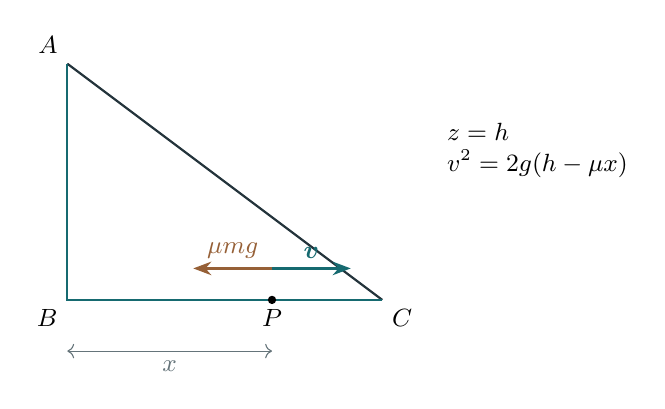
\begin{tikzpicture}
\draw[object] (0,3)--(4,0);\draw[traj] (0,3)--(0,0)--(4,0);
\node[above left] at (0,3) {$A$};\node[below left] at (0,0) {$B$};\node[below right] at (4,0) {$C$};
\fill (2.6,0) circle(1.5pt) node[below] {$P$};
\draw[motion] (2.6,.4)--(3.6,.4) node[midway,above] {$\boldsymbol v$};
\draw[force] (2.6,.4)--(1.6,.4) node[midway,above] {$\mu mg$};
\draw[axis,<->] (0,-.65)--(2.6,-.65) node[midway,below] {$x$};
\node[right,align=left] at (4.7,1.9) {$z=h$\\$v^2=2g(h-\mu x)$};
\end{tikzpicture}
\figcaption{变图1.1V2\quad 在底边运动时，摩擦使速率随已走距离减小}
\end{minipage}\end{center}
任意允许路径有$z\le h$，所以同一$x$处$v\le\sqrt{2g(h-\mu x)}$，其水平时间至少为底边上的积分。竖直段中摩擦已消耗的能量使$v\le\sqrt{2gz}$，竖直总时间至少为$t_1$。底边路径同时取等，
\[
T_{\min}=t_1+\int_0^b\frac{\dd x}{\sqrt{2g(h-\mu x)}}
=t_1+\frac{\sqrt{2gh}-\sqrt{2g(h-\mu b)}}{\mu g}.
\]
$\mu=0$时取连续极限，水平时间恢复为$b/\sqrt{2gh}$。再记$\beta=\mu b/h<1$。三角形内$x\le bz/h$，故$z-\mu x\ge(1-\beta)z$；每个水平微元还有$z-\mu x\ge(h/b-\mu)x$。分别积分可得
\[
T_{\rm v}\le\frac{t_1}{\sqrt{1-\beta}},\qquad
T_{\rm h}\le\frac{b}{\sqrt{1-\beta}}\sqrt{\frac{2}{gh}},\qquad
T_{\sup}=\frac{t_1(1+b/h)}{\sqrt{1-\mu b/h}}.
\]
逐次先下降、后向右的细阶梯使$x$与$bz/h$的差趋零，竖直和水平两项同时趋向上式。条件$\mu<h/b$保证这一极限运动始终有正的重力净作功。

\item \textbf{重力随高度改变。}重力加速度为下降量的函数$g(z)>0$，设$U(z)=\int_0^z g(s)\dd s$。求最快时间与最长时间极限。

变图1.1V3的$P$位于下降量$z$处，竖直箭头表示当地的$g(z)$。能量给$v(z)=\sqrt{2U(z)}$，$U$随$z$严格增大，水平段放得越低，速率越大。
\begin{center}\begin{minipage}{.98\linewidth}\centering
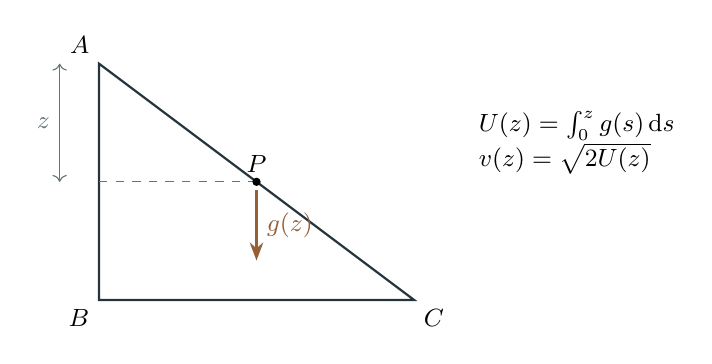
\begin{tikzpicture}
\draw[object] (0,3)--(0,0)--(4,0)--cycle;
\draw[guide] (0,1.5)--(2,1.5);\fill (2,1.5) circle(1.5pt) node[above] {$P$};
\draw[axis,<->] (-.5,3)--(-.5,1.5) node[midway,left] {$z$};
\draw[force] (2,1.4)--(2,.5) node[midway,right] {$g(z)$};
\node[above left] at (0,3) {$A$};\node[below left] at (0,0) {$B$};\node[below right] at (4,0) {$C$};
\node[right,align=left] at (4.7,2) {$U(z)=\int_0^z g(s)\dd s$\\$v(z)=\sqrt{2U(z)}$};
\end{tikzpicture}
\figcaption{变图1.1V3\quad 当地速率由从A下降到该高度的重力作功确定}
\end{minipage}\end{center}
所有竖直段的时间仍合成为同一个积分。水平微元在$x$处的下降量满足$hx/b\le z\le h$，因此
\[
\frac{b}{\sqrt{2U(h)}}\le T_{\rm h}
\le\int_0^b\frac{\dd x}{\sqrt{2U(hx/b)}}
=\frac bh\int_0^h\frac{\dd z}{\sqrt{2U(z)}}.
\]
底边路径达到最短时间，细阶梯逼近最长时间极限：
\[
T_{\min}=\int_0^h\frac{\dd z}{\sqrt{2U(z)}}+\frac b{\sqrt{2U(h)}},\qquad
T_{\sup}=\left(1+\frac bh\right)\int_0^h\frac{\dd z}{\sqrt{2U(z)}}.
\]
从静止出发能否在有限时间内完成下落，由共同的竖直积分决定。若$g(z)$在起点趋向正的有限值$g(0)$，则$U(z)\sim g(0)z$，积分核按$z^{-1/2}$变化。一般地，若$U(z)\sim az^p$，其中$a>0$，则起点附近的积分核正比于$z^{-p/2}$，故积分在$p<2$时收敛。若$p\ge2$，竖直积分已经发散，所有允许路径都无有限到达时间。

\item \textbf{把直角拐折换成光滑圆弧。}用半径$a$的四分之一圆弧连接竖直段与水平段，$0<a<\min(h,b)$，求这条路径的时间及$a\to0$的极限。

变图1.1V4中，圆弧在$P=(0,a)$与竖直段相切，在$Q=(a,0)$与水平段相切，圆心为$O_a=(a,a)$。各处速率仍由下降高度决定。
\begin{center}\begin{minipage}{.98\linewidth}\centering
\begin{tikzpicture}
\draw[guide] (0,3)--(0,0)--(4,0);\draw[object] (0,3)--(4,0);
\draw[traj] (0,3)--(0,.8) arc(180:270:.8)--(4,0);
\draw[guide] (0,.8)--(.8,.8)--(.8,0);
\fill (.8,.8) circle(1.2pt) node[above right] {$O_a$};
\node[left] at (0,.8) {$P$};\node[below] at (.8,0) {$Q$};
\node[above left] at (0,3) {$A$};\node[below left] at (0,0) {$B$};\node[below right] at (4,0) {$C$};
\node[above] at (.4,.8) {$a$};\node[right] at (.8,.4) {$a$};
\node[right,align=left] at (4.7,1.9) {圆弧长为$\pi a/2$\\弧上下降量持续增大};
\end{tikzpicture}
\figcaption{变图1.1V4\quad 有限圆弧同时替代一段竖直路程和一段水平路程}
\end{minipage}\end{center}
弧上取$0\le\phi\le\pi/2$，
\[
x=a(1-\cos\phi),\qquad y=a(1-\sin\phi),\qquad
z=h-a+a\sin\phi,\qquad \dd s=a\dd\phi.
\]
所以弧段时间及全程时间为
\[
T_{\mathrm{arc}}=\int\frac{\dd s}{\sqrt{2gz(s)}}
=a\int_0^{\pi/2}\frac{\dd\phi}{\sqrt{2g(h-a+a\sin\phi)}},
\]
\[
T(a)=\sqrt{\frac{2(h-a)}g}+T_{\mathrm{arc}}+
\frac{b-a}{\sqrt{2gh}}.
\]
第一项沿$AP$从静止下落，末项沿$QC$以末速匀速运动。随$a\to0$，弧长和弧段时间趋零，两直线段长度趋于$h,b$，故$T(a)\to t_1+t_2$。若第一问只给这条圆弧路径与$AC$等时，则有限$a$时应使用$T(a)$；在$a\to0$时恢复$\sin\alpha+\cos\alpha/2=1$。

\item \textbf{带非零初速进入路径。}质点在$A$处的初速大小为$u_0>0$，转弯保速。求最快路径和全过程时间。

下降量$z$处的速率为$v(z)=\sqrt{u_0^2+2gz}$。变图1.1V5比较同一小段水平距离分别放在$P$、底边上的用时；底边速率$v_h=\sqrt{u_0^2+2gh}$最大。
\begin{center}\begin{minipage}{.98\linewidth}\centering
\begin{tikzpicture}
\draw[object] (0,3)--(0,0)--(4,0)--cycle;
\draw[motion] (.1,2.9)--(.1,2.2) node[right] {$u_0$};
\draw[thick,color=warm] (.8,1.5)--(1.6,1.5);\draw[motion] (.9,1.8)--(1.5,1.8);
\node[above] at (1.2,1.9) {$P:\ v(z)$};
\draw[traj] (.8,0)--(1.6,0);\draw[motion] (.9,.3)--(1.5,.3);
\node[below] at (1.2,-.1) {$v_h$};
\node[above left] at (0,3) {$A$};\node[below left] at (0,0) {$B$};\node[below right] at (4,0) {$C$};
\node[right,align=left] at (4.7,1.8) {两水平段长度相同\\$v(z)\le v_h$};
\end{tikzpicture}
\figcaption{变图1.1V5\quad 非零初速保留了速率随下降量增大的次序}
\end{minipage}\end{center}
任意路径的竖直时间为
\[
T_{\mathrm v}=\int_0^h\frac{\dd z}{\sqrt{u_0^2+2gz}}
=\frac{\sqrt{u_0^2+2gh}-u_0}{g}.
\]
每个水平微元的耗时至少为$\dd x/v_h$，将它们全部放在底边即可取等。因此最快路径仍为$A\to B\to C$，
\[
T_{\min}=\frac{v_h-u_0}{g}+\frac b{v_h}.
\]
$u_0\to0$时，两项分别恢复自由落体时间和底边匀速时间。

\item \textbf{有限阶梯离最长时间还有多远。}每次先下降$h/N$、再向右$b/N$，求总时间，并估计趋近最长时间极限的误差。

变图1.1V6中第$k$段水平路程位于$z_k=kh/N$，速率$v_k=\sqrt{2gkh/N}$，每段长度为$b/N$。
\begin{center}\begin{minipage}{.98\linewidth}\centering
\begin{tikzpicture}
\draw[object] (0,3)--(0,0)--(4,0)--cycle;
\draw[traj] (0,3)\foreach \j in {1,...,4}{--({\j-1},{3-.75*\j})--({\j},{3-.75*\j})};
\draw[axis,<->] (1,1.15)--(2,1.15) node[midway,below] {$b/N$};
\draw[axis,<->] (-.5,3)--(-.5,2.25) node[midway,left] {$h/N$};
\node[above left] at (0,3) {$A$};\node[below left] at (0,0) {$B$};\node[below right] at (4,0) {$C$};
\node[right,align=left] at (4.7,1.9) {图取$N=4$\\第$k$水平段：$z_k=kh/N$};
\end{tikzpicture}
\figcaption{变图1.1V6\quad 每级的速率在该级水平段上保持常量}
\end{minipage}\end{center}
竖直时间仍为$t_1$，故
\[
T_N=t_1+\frac b{\sqrt{2gh}}\frac1{\sqrt N}
\sum_{k=1}^Nk^{-1/2}.
\]
用递减函数的积分夹住求和，
\[
2(\sqrt{N+1}-1)\le\sum_{k=1}^Nk^{-1/2}
\le2\sqrt N-1.
\]
记$K=b/\sqrt{2gh}$，则
\[
\frac K{\sqrt N}\le T_{\sup}-T_N
\le\frac{2K}{\sqrt N}
\left(1+\sqrt N-\sqrt{N+1}\right)
<\frac{2K}{\sqrt N}.
\]
误差具有$N^{-1/2}$的尺度。将级数增到约四倍，可把同一误差尺度减为原来的一半；起点附近速率小，正是收敛较慢的部分。

\item \textbf{非零初速下的最长时间极限。}仍取变式5的初速$u_0>0$，求细阶梯用时极限及其与最短用时之比。

变图1.1V7在斜边上选$P$，其对应下降量为$z=hx/b$。细阶梯的水平段从斜边内侧趋近$P$，故水平时间的极限为
\[
T_{{\rm h},\sup}=\int_0^b\frac{\dd x}{\sqrt{u_0^2+2ghx/b}}
=\frac bh\frac{v_h-u_0}{g}.
\]
\begin{center}\begin{minipage}{.98\linewidth}\centering
\begin{tikzpicture}
\draw[object] (0,3)--(0,0)--(4,0)--cycle;
\draw[traj] (0,3)\foreach \j in {1,...,6}{--({2*(\j-1)/3},{3-.5*\j})--({2*\j/3},{3-.5*\j})};
\fill (2,1.5) circle(1.4pt) node[above right] {$P$};
\draw[guide] (0,1.5)--(2,1.5)--(2,0);
\draw[axis,<->] (-.5,3)--(-.5,1.5) node[midway,left] {$z=hx/b$};
\node[above left] at (0,3) {$A$};\node[below left] at (0,0) {$B$};\node[below right] at (4,0) {$C$};
\node[right,align=left] at (4.7,1.8) {$v_P=\sqrt{u_0^2+2ghx/b}$\\有限阶梯从斜边内侧逼近};
\end{tikzpicture}
\figcaption{变图1.1V7\quad 斜边位置给出每个水平微元可处的最高位置}
\end{minipage}\end{center}
再加竖直时间$T_{\rm v}=(v_h-u_0)/g$，得
\[
T_{\sup}=\left(1+\frac bh\right)\frac{v_h-u_0}{g},\qquad
\frac{T_{\sup}}{T_{\min}}
=\frac{2v_h(h+b)}{2hv_h+b(v_h+u_0)}.
\]
这里用到$v_h-u_0=2gh/(v_h+u_0)$。取$b/h=4/3$，$u_0\to0$时比值趋于$7/5$；$u_0^2\gg2gh$时各高度速率趋近同一个$u_0$，竖直与水平总路程分别固定，比值趋于1。

\item \textbf{把可走区域改成矩形。}允许路径位于宽$b$、高$h$的矩形内，仍只向下、向右，质点在左上角$A$从静止出发到右下角$C$。求最快时间，讨论用时能否任意大。

底边路径仍使所有水平微元以最大速率通过，最短时间保持$t_1+b/\sqrt{2gh}$。变图1.1V8另构造一条路径：先下降$\delta>0$，横穿全部宽度$b$，再下降到$C$。
\begin{center}\begin{minipage}{.98\linewidth}\centering
\begin{tikzpicture}
\draw[object] (0,3)--(0,0)--(4,0)--(4,3)--cycle;
\draw[traj] (0,3)--(0,2.55)--(4,2.55)--(4,0);
\node[above left] at (0,3) {$A$};\node[below left] at (0,0) {$B$};\node[below right] at (4,0) {$C$};
\draw[axis,<->] (-.5,3)--(-.5,2.55) node[midway,left] {$\delta$};
\draw[motion] (1,2.55)--(2.2,2.55) node[midway,above] {$\sqrt{2g\delta}$};
\draw[axis,<->] (0,-.5)--(4,-.5) node[midway,below] {$b$};
\node[right,align=left] at (4.7,1.8) {先小幅下落，再横穿矩形\\水平段可保持很小的速率};
\end{tikzpicture}
\figcaption{变图1.1V8\quad 矩形允许在任意小的下降量处完成全部水平位移}
\end{minipage}\end{center}
两段竖直时间之和为$t_1$，中间水平速率保持$\sqrt{2g\delta}$，所以
\[
T(\delta)=t_1+\frac b{\sqrt{2g\delta}}
\longrightarrow+\infty\qquad(\delta\to0^+).
\]
每条$\delta>0$的路径都从先下落获得正速率，运动可完成。三角形中的斜边曾给出$z\ge hx/b$；矩形允许横穿段任意接近$A$的高度，故这一组允许路径的用时没有有限上界。
\end{enumerate}


\clearpage

\pdfbookmark[2]{第 2 题 线性阻力下的剩余路程}{q2}

\section*{第 2 题\quad 线性阻力下的剩余路程}

\tagline{M-01-02}

质量为 $m$ 的质点以初速度 $v_0>0$ 沿 $x$ 轴正方向运动，初始位置为 $x=0$。唯一的运动方向上的力为线性阻力 $F_x=-bv$，其中 $b>0$ 为常量。

当速度降为 $v_0/n$（$n>1$）时，求已通过路程与总路程之比。总路程指 $t\to\infty$ 时路程的极限。

\begin{center}
\begin{tikzpicture}
\draw[axis] (-.7,0)--(7.0,0) node[right] {$x$};
\fill[ink] (2.7,0) circle (2.5pt);\node[below] at (2.7,-.12) {$m$};
\draw[motion] (2.7,.4)--(4.6,.4) node[above] {$\vect v$};
\draw[force] (2.7,.4)--(1.0,.4) node[above] {$\vect F$};
\draw (0,.1)--(0,-.1);\node[below] at (0,-.1) {$O$};
\node[color=muted] at (3.4,1.25) {阻力始终与速度反向};
\end{tikzpicture}
\figcaption{图 1.2\quad 运动方向与阻力方向。}
\end{center}

\Needspace{5\baselineskip}

\pdfbookmark[3]{题型定位}{q2-h0}

\subsection*{题型定位}

线性阻力下的速度衰减与剩余路程。求 $v(t)$ 后积分得到有限总路程，再消去时间建立 $v(x)$；区分无限衰减时间与有限位移极限。

\Needspace{5\baselineskip}

\pdfbookmark[3]{知识点}{q2-h1}

\subsection*{知识点}

\begin{itemize}
\item 线性阻力$F_x=-bv$给$\dot v=-kv$，$k=b/m$是衰减率。
\item 分离变量从$v_0$到$v$积分得到无量纲对数$\ln(v/v_0)=-kt$。
\item 位置由速度积分得到，初始条件$x(0)=0$确定积分常数。
\item 在正速度区间使用$\dot v=v\dd v/\dd x$，可得到速度—位置直线。
\item 速度曲线下的未来面积给剩余路程$v/k$，全部面积给总路程极限$v_0/k$。
\end{itemize}
解图1.2A的横轴是时间，曲线斜率为加速度；解图1.2B的横轴是位置，斜率为$\dd v/\dd x=-k$。两图分别呈指数与直线，描述同一运动。


\Needspace{5\baselineskip}

\pdfbookmark[3]{物理图像}{q2-h2}

\subsection*{物理图像}

题图中速度向右、阻力向左。速度减小时阻力也减小，减速过程逐步放缓。解图1.2A中$v/v_0=e^{-kt}$在有限时刻保持正值，曲线下的总面积收敛到$x_m$；从当前时刻向右的面积则是剩余路程。解图1.2B将这一过程改画在速度—位置平面，当前点沿直线趋向横轴截距$x_m$。截距到当前横坐标的距离为$v/k$，因此速度比例与剩余路程比例相同。

\Needspace{5\baselineskip}

\pdfbookmark[3]{解题入口}{q2-h3}

\subsection*{解题入口}

先由题设$F_x=-bv$除以质量，记$k=b/m$，得到$\dot v=-kv$。从初值积分求$v(t)$，随后将速度从0积分到$t$，再令$t\to\infty$求总路程极限。指定$v=v_0/n$时，速度式和位置式中使用同一个指数因子$1/n$。

也可由$\dot v=v\dd v/\dd x$进入。在$v>0$的运动区间内约去$v$，得到$\dd v/\dd x=-k$，由初值求直线$v=v_0-kx$。这条直线将已走路程、剩余路程和当前速度直接联系起来，时间法则同时说明趋近过程。

\Needspace{5\baselineskip}

\pdfbookmark[3]{标准解法}{q2-h4}

\subsection*{标准解法}

取初速度方向为 $x$ 轴正向，记 $k=b/m>0$。题图 1.2 中速度向右、阻力向左，运动方程为
\[
m\dot v=-bv,\qquad\dot v=-kv,\qquad v(0)=v_0.
\]
\subsubsection*{速度与位置随时间变化}
在 $v>0$ 的运动区间内分离变量，由初始时刻积分到 $t$，
\[
\int_{v_0}^{v(t)}\frac{\dd u}{u}
=-k\int_0^t\dd s,
\qquad\ln\frac{v(t)}{v_0}=-kt.
\]
所以
\[
\boxed{v(t)=v_0e^{-kt}},\qquad
x(t)=\int_0^t v_0e^{-ks}\dd s
=\boxed{\frac{v_0}{k}(1-e^{-kt})}.
\]
速度在任意有限时刻都为正，故位移等于已通过路程。解图 1.2A 的速度曲线无限延伸，但曲线下的总面积收敛：
\begin{center}\begin{minipage}{\linewidth}\centering\begin{tikzpicture}

\draw[axis] (-.2,0)--(5,0) node[right] {$t$};\draw[axis] (0,-.15)--(0,2.65) node[above] {$v$};
\fill[accent!12] ({ln(3)},0)--plot[domain={ln(3)}:4.6,samples=70](\x,{2.2*exp(-\x)})--(4.6,0)--cycle;
\draw[traj,domain=0:4.6,samples=80] plot(\x,{2.2*exp(-\x)});
\draw[guide] ({ln(3)},0)--({ln(3)},{2.2*(1/3)})--(0,{2.2*(1/3)});
\node[left] at (0,2.2) {$v_0$};\node[left] at (0,{2.2*(1/3)}) {$v_0/n$};\node[below] at ({ln(3)},0) {$t_n$};
\node[align=left] at (6.75,1.75) {全部曲线下面积：$x_m$\\$t_n$ 后的面积：剩余路程\\$v(t)=v_0e^{-kt}$};
\draw[thin] (1.62,.25)--(3.0,1.02) node[right] {$x_m-x_n$};

\end{tikzpicture}
\figcaption{解图 1.2A\quad 速度曲线下面积等于路程；阴影部分对应速度已降至 $v_0/n$ 后的剩余路程。}
\end{minipage}\end{center}
\[
x_m=\int_0^\infty v_0e^{-kt}\dd t=\frac{v_0}{k}.
\]
$x_m$ 是无限时间下的路程极限；任意有限时刻仍有 $x<x_m,v>0$。
\subsubsection*{代入指定速度比例}
令 $v(t_n)=v_0/n$，则
\[
e^{-kt_n}=\frac1n,\qquad t_n=\frac{\ln n}{k}.
\]
此时
\[
x_n=\frac{v_0}{k}\left(1-\frac1n\right),\qquad
\boxed{\frac{x_n}{x_m}=1-\frac1n}.
\]
$n\to1^+$ 时，指定时刻趋于零，已走路程比例也趋于零；$n\to\infty$ 时，比例趋于一，所需时间却趋于无穷。
\subsubsection*{速度与位置的直接关系}
由于 $\dot v=v\,\dd v/\dd x$，运动方程还可写为
\[
v\frac{\dd v}{\dd x}=-kv.
\]
在 $v>0$ 时约去 $v$，从 $x=0,v=v_0$ 积分，得
\[
v=v_0-kx,\qquad
\boxed{\frac{v}{v_0}+\frac{x}{x_m}=1}.
\]
\begin{center}\begin{minipage}{\linewidth}\centering\begin{tikzpicture}

\draw[axis] (-.15,0)--(4.65,0) node[right] {$x$};\draw[axis] (0,-.15)--(0,2.7) node[above] {$v$};
\draw[traj] (0,2.2)--(4,0);\node[left] at (0,2.2) {$v_0$};\node[below] at (4,0) {$x_m$};
\fill ({8/3},{2.2/3}) circle(2pt);\draw[guide] ({8/3},0)--({8/3},{2.2/3})--(0,{2.2/3});
\node[below] at ({8/3},0) {$x_n$};\node[left] at (0,{2.2/3}) {$v_0/n$};
\node[align=left] at (6.7,1.65) {$\displaystyle\frac{v}{v_0}+\frac{x}{x_m}=1$\\[4pt]$x_m-x=\dfrac vk$};

\end{tikzpicture}
\figcaption{解图 1.2B\quad 消去时间后，$v$ 与 $x$ 成线性关系。由图中截距和当前点直接读出路程比例。}
\end{minipage}\end{center}
两张解图都取 $n=3$。在解图 1.2A 中，竖线经过 $kt_n=\ln3$，此处速度为 $v_0/3$。解图 1.2B 的同一时刻对应直线上的点 $(2x_m/3,v_0/3)$，距横轴截距还有 $x_m/3$。直线上任意一点的横坐标到截距的距离都是 $x_m-x=v/k$。$v$ 随时间指数衰减，随位置却线性减小；两种关系的自变量不同。
\subsubsection*{积分常数与当前状态之后的运动}
若用不定积分求位置，先得到
\[
x=-\frac{v_0}{k}e^{-kt}+C_x.
\]
将$x(0)=0$代入上式，常量项与初始指数项相抵，得到$C_x=v_0/k$。
从 $v_0$ 积到 $v$，得到 $\ln(v/v_0)$。对数的真数是速度之比，初始速度由积分下限给定。
在解图1.2A的指定时刻$t_n$之后，令$\tau=t-t_n$，
则$v(t_n+\tau)=(v_0/n)e^{-k\tau}$，因此
\[
x_m-x_n=\int_0^\infty\frac{v_0}{n}e^{-k\tau}\dd\tau
=\frac{v_0}{nk}.
\]
它恰是解图1.2B中当前点到横轴截距的水平距离。
在$t_n$之后，速度与剩余路程按同一个指数因子继续减小。每经历$\ln2/k$的时间，二者均减半；随$t\to\infty$，速度趋零，位置趋于有限的$x_m$。


\Needspace{5\baselineskip}

\pdfbookmark[3]{关键洞察}{q2-h5}

\subsection*{关键洞察}

线性阻力使未来运动在任意当前状态都具有相同形式：当前速度为$v$时，之后的速度为$ve^{-ks}$，剩余路程便为$v/k$。因此速度降至$v_0/n$时，剩余比例为$1/n$，已走比例为$1-1/n$。速度减半时已走一半路程，速度降为十分之一时已走九成；每再走完剩余路程的一半，都经历相同的$\ln2/k$。变式3进一步比较代数衰减尾部，说明总路程由速度的时间积分是否收敛决定。

\Needspace{5\baselineskip}

\pdfbookmark[3]{易错点}{q2-h6}

\subsection*{易错点}

\begin{itemize}
\item 阻力沿$-x$，方程和指数均带负号，$\dot v=-kv$、$v=v_0e^{-kt}$。
\item 由$x(0)=0$确定位置积分中的$C_x=v_0/k$，使位置从给定原点开始。
\item 位移等于路程的依据是全过程$v>0$；总路程为$t\to\infty$时的极限。
\item $n\to1^+$时指定时刻与已走比例均趋零，$n\to\infty$时已走比例趋1、时刻趋于无穷。
\item $v(x)$的横轴是位置，直线截距给总路程；$v(t)$的横轴是时间，曲线下面积才给路程。
\end{itemize}

\Needspace{5\baselineskip}

\pdfbookmark[3]{课堂讲解建议}{q2-h7}

\subsection*{课堂讲解建议}

先问：“速度减到一半时，走完的路程占多少？”让学生保留$v(t),x(t),x_m$三式，再由$v/v_0+x/x_m=1$回答恰好一半。接着问：“已走四分之三时，速度和剩余路程各是多少？”在解图1.2B定位当前点，分别读出$v_0/4$与$x_m/4$。

用解图1.2A的未来面积求剩余路程，再追问“走完下一半剩余路程要多久”。从当前速度重新积分，得到每次均为$\ln2/k$，而对应路程逐次减半。将变式3的代数衰减曲线并排比较，让学生从积分判断哪一种总面积有限。最后用等时间隔的位移增量反求$k$，说明同一指数规律怎样从位置记录中识别出来。

\Needspace{5\baselineskip}

\pdfbookmark[3]{变式训练}{q2-h8}

\subsection*{变式训练}

\begin{enumerate}
\item \textbf{速度降为十分之一。}求此时的路程比例、经历时间及剩余路程。

令$\tau=kt$，由$v/v_0=e^{-\tau}$，指定速度给$\tau=\ln10$。将同一个指数因子代入位置式，
\[
t=\frac{\ln10}{k},\qquad x=\frac{v_0}{k}\left(1-\frac1{10}\right),\qquad
\frac{x}{x_m}=\frac9{10},\quad x_m-x=\frac{x_m}{10}.
\]
变图1.2V1在同一时间轴画速度比例与路程比例。两条曲线在任意时刻的纵坐标之和为1；$\tau=\ln10$的竖线分别与它们交于$1/10$和$9/10$。
\begin{center}\begin{minipage}{.98\linewidth}\centering
\begin{tikzpicture}
\draw[axis] (0,0)--(5.6,0) node[right] {$\tau=kt$};\draw[axis] (0,0)--(0,3.1) node[above] {比值};
\draw[traj,domain=0:5,samples=60] plot(\x,{2.6*exp(-\x)});
\draw[thick,dashed,color=warm,domain=0:5,samples=60] plot(\x,{2.6*(1-exp(-\x))});
\draw[guide] ({ln(10)},0)--({ln(10)},2.6);
\node[below] at ({ln(10)},0) {$\ln10$};\node[left] at (0,2.6) {$1$};
\fill ({ln(10)},.26) circle(1.5pt);\fill ({ln(10)},2.34) circle(1.5pt);
\node[right] at (3.3,.35) {$v/v_0$};\node[right,color=warm] at (3.3,2.25) {$x/x_m$};
\end{tikzpicture}
\figcaption{变图1.2V1\quad 指定同一时刻，速度比例与路程比例互补}
\end{minipage}\end{center}
此后速度继续指数减小，剩余的十分之一路程由$t$之后的速度曲线面积给出。

\item \textbf{已经走完四分之三。}求该时刻速度、时间和剩余路程。

从运动方程用$\dot v=v\dd v/\dd x$消去时间，得到$\dd v/\dd x=-k$，初值积分后有$v=v_0-kx$。取$x=3x_m/4$、$x_m=v_0/k$，
\[
v=\frac{v_0}{4},\qquad e^{-kt}=\frac14,\qquad
t=\frac{\ln4}{k},\qquad x_m-x=\frac{x_m}{4}.
\]
变图1.2V2的$P$在速度—位置直线上，横坐标$3/4$、纵坐标$1/4$；从$P$向横轴截距量得的水平距离就是剩余路程比例。
\begin{center}\begin{minipage}{.98\linewidth}\centering
\begin{tikzpicture}
\draw[axis] (0,0)--(5.2,0) node[right] {$x/x_m$};\draw[axis] (0,0)--(0,3.1) node[above] {$v/v_0$};
\draw[traj] (0,2.6)--(4,0);\fill (3,.65) circle(1.6pt) node[above right] {$P$};
\draw[guide] (3,0)--(3,.65)--(0,.65);
\node[below] at (3,0) {$3/4$};\node[below] at (4,0) {$1$};\node[left] at (0,.65) {$1/4$};\node[left] at (0,2.6) {$1$};
\draw[axis,<->] (3,-.65)--(4,-.65) node[midway,below] {$1/4$};
\end{tikzpicture}
\figcaption{变图1.2V2\quad 已走路程确定当前速度，横轴上还余四分之一}
\end{minipage}\end{center}

\item \textbf{改用三次阻力。}设运动方程为$\dot v=-\kappa v^3$，$\kappa>0$，初值仍为$v_0$。求速度和路程，比较总路程的收敛性。

分离变量并积分，
\[
\int_{v_0}^{v}u^{-3}\dd u=-\kappa t,
\qquad v(t)=\frac{v_0}{\sqrt{1+2\kappa v_0^2t}}.
\]
再积分速度，得到
\[
x(t)=\frac{\sqrt{1+2\kappa v_0^2t}-1}{\kappa v_0},\qquad
v(t)\sim(2\kappa t)^{-1/2}.
\]
路程随$\sqrt t$增长，因而总路程无界。变图1.2V3为便于比较，取$\kappa v_0^2=k$，使两种阻力的初始减速度相同；横轴都用$\tau=kt$。三次阻力的代数尾部比线性阻力的指数尾部衰减慢，其速度曲线下面积随时间持续增大。
\begin{center}\begin{minipage}{.98\linewidth}\centering
\begin{tikzpicture}
\draw[axis] (0,0)--(5.5,0) node[right] {$\tau=kt$};\draw[axis] (0,0)--(0,3.1) node[above] {$v/v_0$};
\draw[traj,domain=0:5,samples=60] plot(\x,{2.6*exp(-\x)});
\draw[thick,dashed,color=warm,domain=0:5,samples=60] plot(\x,{2.6/sqrt(1+2*\x)});
\node[left] at (0,2.6) {$1$};\node[below] at (0,0) {$0$};
\node[right,color=warm] at (3.4,1.4) {三次阻力};\node[right] at (3.4,.3) {线性阻力};
\end{tikzpicture}
\figcaption{变图1.2V3\quad 初始减速度相同，后期速度的衰减规律不同}
\end{minipage}\end{center}
这里$k$的单位为$\mathrm{s^{-1}}$，$\kappa$的单位为$\mathrm{s\,m^{-2}}$；两者分别与各自的速度幂次组合，给出加速度。

\item \textbf{阻力系数加倍。}保持$m,v_0$不变，将$b$改为$2b$。比较降到同一速度比例时的时间、路程、总路程及路程比例。

新衰减率为$k'=2k$，故$v'(t)=v_0e^{-2kt}$。指定$v'=v_0/n$时，
\[
t_n'=\frac{\ln n}{2k}=\frac{t_n}{2},\qquad
x_n'=\frac{v_0}{2k}\left(1-\frac1n\right)=\frac{x_n}{2},\qquad
x_m'=\frac{x_m}{2}.
\]
两种路程都减半，因此$x_n'/x_m'=1-1/n$保持。变图1.2V4用相同的实际时间单位$1/k$比较两条速度曲线，新曲线达到同一纵坐标时所需横坐标减半。
\begin{center}\begin{minipage}{.98\linewidth}\centering
\begin{tikzpicture}
\draw[axis] (0,0)--(5.5,0) node[right] {$kt$};\draw[axis] (0,0)--(0,3.1) node[above] {$v/v_0$};
\draw[traj,domain=0:5,samples=60] plot(\x,{2.6*exp(-\x)});
\draw[thick,dashed,color=warm,domain=0:5,samples=60] plot(\x,{2.6*exp(-2*\x)});
\draw[guide] (0,.65)--({ln(4)},.65);\draw[guide] ({ln(4)},0)--({ln(4)},.65);\draw[guide] ({ln(4)/2},0)--({ln(4)/2},.65);
\node[left] at (0,.65) {$1/4$};\node[left] at (0,2.6) {$1$};
\node[below] at ({ln(4)/2},0) {$\frac12\ln4$};\node[below] at ({ln(4)},-.55) {$\ln4$};
\node[right] at (3.3,1.4) {实线：$b$};\node[right,color=warm] at (3.3,.9) {虚线：$2b$};
\end{tikzpicture}
\figcaption{变图1.2V4\quad 加倍阻力系数使达到同一速度比例的时间减半}
\end{minipage}\end{center}

\item \textbf{从当前状态求剩余路程。}在任意时刻$t_*$，质点速度为$v_*>0$，位置为$x_*$。以该时刻为新的时间起点，直接求后续路程。

令$s=t-t_*$，方程与初值为$\dd v/\dd s=-kv$、$v(0)=v_*$，因此$v(s)=v_*e^{-ks}$。对未来全部时间积分，
\[
\Delta x_{\rm rem}=\int_0^\infty v_*e^{-ks}\dd s=\frac{v_*}{k},\qquad
x_*+\frac{v_*}{k}=x_m.
\]
变图1.2V5画的是从$t_*$起重新计时的速度曲线，阴影随曲线向右延伸，整个面积为$v_*/k$。剩余路程与当前速度成正比，所以每当剩余路程减半，当前速度也减半，所需时间均为$\ln2/k$。
\begin{center}\begin{minipage}{.98\linewidth}\centering
\begin{tikzpicture}
\fill[accent!12] (0,0)--(0,2.6)--plot[domain=0:5,samples=60](\x,{2.6*exp(-\x)})--(5,0)--cycle;
\draw[axis] (0,0)--(5.5,0) node[right] {$ks$};\draw[axis] (0,0)--(0,3.1) node[above] {$v/v_*$};
\draw[traj,domain=0:5,samples=60] plot(\x,{2.6*exp(-\x)});
\draw[motion] (4.4,{2.6*exp(-4.4)})--(5,{2.6*exp(-5)});
\node[left] at (0,2.6) {$1$};\node[below] at (0,0) {$0$};
\node[right,align=left] at (2.5,1.65) {面积乘$v_*/k$\\即为剩余路程};
\end{tikzpicture}
\figcaption{变图1.2V5\quad 当前状态作为初态，未来速度曲线决定剩余路程}
\end{minipage}\end{center}

\item \textbf{阻力消耗的机械能。}求速度降至$v_0/n$时损失的动能，以及此后还将损失的动能。

阻力瞬时功率为$P_F=-bv^2$。动能方程给$\dot K=-bv^2$，代入$v=v_0e^{-kt}$，从0积分到$t_n$：
\[
K_0-K(t_n)=\int_0^{t_n}bv_0^2e^{-2kt}\dd t
=\frac12mv_0^2\left(1-\frac1{n^2}\right).
\]
此后还将损失当前全部动能$K(t_n)=mv_0^2/(2n^2)$。变图1.2V6在横轴$x/x_m$上画$K/K_0=(1-x/x_m)^2$，所以路程已走比例与动能已损失比例各有不同函数关系。例如速度减半时已走一半路程，已损失四分之三动能。
\begin{center}\begin{minipage}{.98\linewidth}\centering
\begin{tikzpicture}
\draw[axis] (0,0)--(5.2,0) node[right] {$x/x_m$};\draw[axis] (0,0)--(0,3.1) node[above] {$K/K_0$};
\draw[traj,domain=0:1,samples=60] plot({4*\x},{2.6*(1-\x)^2});
\fill (2,.65) circle(1.5pt);\draw[guide] (2,0)--(2,.65)--(0,.65);
\node[below] at (2,0) {$1/2$};\node[below] at (4,0) {$1$};\node[left] at (0,.65) {$1/4$};\node[left] at (0,2.6) {$1$};
\end{tikzpicture}
\figcaption{变图1.2V6\quad 速度随位置线性下降，动能随位置按平方下降}
\end{minipage}\end{center}

\item \textbf{增加恒定驱动力。}在同一线性阻力之外施加沿$+x$的恒力$F_0>0$，求速度与位置随时间的变化。

运动方程为$m\dot v=F_0-bv$，记$v_\infty=F_0/b$。令$w=v-v_\infty$，方程化为$\dot w=-kw$，用初始速度积分得
\[
v(t)=v_\infty+(v_0-v_\infty)e^{-kt},\qquad
x(t)=v_\infty t+\frac{v_0-v_\infty}{k}(1-e^{-kt}).
\]
变图1.2V7示例取$v_0=2v_\infty$，速度从较大初值趋向终端速率。到达终端状态附近时驱动力与阻力的大小趋于相等，位置包含持续增长的$v_\infty t$，故全程路程随时间无界增加。
\begin{center}\begin{minipage}{.98\linewidth}\centering
\begin{tikzpicture}
\draw[axis] (0,0)--(5.5,0) node[right] {$kt$};\draw[axis] (0,0)--(0,3.1) node[above] {$v/v_\infty$};
\draw[traj,domain=0:5,samples=60] plot(\x,{1.3*(1+exp(-\x))});
\draw[guide] (0,1.3)--(5.1,1.3);\node[left] at (0,1.3) {$1$};\node[left] at (0,2.6) {$2$};
\node[right] at (3.2,2.3) {$F_0=bv_\infty$};
\end{tikzpicture}
\figcaption{变图1.2V7\quad 恒力驱动时速度趋于正的终端值}
\end{minipage}\end{center}

\item \textbf{由等时间隔的位置反求阻力。}以相同时间间隔$\Delta t$记录$x_0=0,x_1,x_2,x_3$，质量$m$已知。用前两个位移增量求$k,b,v_0$，并说明第三个增量的关系。

记$d_j=x_j-x_{j-1}$，令$q=e^{-k\Delta t}\in(0,1)$。对每一时间间隔积分速度，
\[
d_j=\frac{v_0}{k}(1-q)q^{j-1},\qquad
q=\frac{d_2}{d_1},\qquad
k=-\frac{\ln q}{\Delta t},\quad b=mk,\quad
v_0=\frac{kd_1}{1-q}.
\]
变图1.2V8取$q=1/2$，连续的位移增量依次减半。等时间隔使指数衰减转为等比数列，所以第三个增量满足$d_3=qd_2=d_2^2/d_1$；它还给出三次记录之间的同一模型关系。
\begin{center}\begin{minipage}{.98\linewidth}\centering
\begin{tikzpicture}
\draw[axis] (-.2,0)--(6.2,0) node[right] {$x$};
\foreach \p/\j in {0/0,3/1,4.5/2,5.25/3}{\fill (\p,0) circle(1.5pt) node[above] {$x_\j$};}
\draw[axis,<->] (0,-.5)--(3,-.5) node[midway,below] {$d_1$};
\draw[axis,<->] (3,-1)--(4.5,-1) node[midway,below] {$d_2$};
\draw[axis,<->] (4.5,-1.5)--(5.25,-1.5) node[midway,below] {$d_3$};
\node[above] at (2.8,1.1) {相邻记录相隔同一$\Delta t$；图取$q=1/2$};
\end{tikzpicture}
\figcaption{变图1.2V8\quad 位移增量的公比给出指数衰减率}
\end{minipage}\end{center}
\end{enumerate}


\clearpage

\pdfbookmark[2]{第 3 题 三次阻力运动规律}{q3}

\section*{第 3 题\quad 三次阻力运动规律}

\tagline{M-01-03}

质量为 $m$ 的质点以初速度 $v_0>0$ 沿 $x$ 轴正方向作直线运动，初始位置为 $x(0)=0$。唯一的运动方向上的力为 $F_x=-cv^3$，其中 $c>0$ 为常量。记 $k=c/m$。
\begin{enumerate}
\item 求速度 $v(t)$ 和位置 $x(t)$；
\item 求速度随位置的变化规律 $v(x)$；
\item 判断总路程是否有限，并说明理由。
\end{enumerate}

\begin{center}
\begin{tikzpicture}
\draw[axis] (-.4,0)--(7.0,0) node[right] {$x$};
\fill[ink] (3,0) circle (2.5pt);\node[below] at (3,-.12) {$m$};
\draw[motion] (3,.4)--(4.6,.4) node[above] {$\vect v$};
\draw[force] (3,.4)--(1.3,.4) node[above] {$F_x=-cv^3$};
\node[color=muted] at (3.4,1.35) {规定 $x(0)=0,\quad v(0)=v_0$};
\draw (0,.1)--(0,-.1);\node[below] at (0,-.1) {$O$};
\end{tikzpicture}
\figcaption{图 1.3\quad 初始速度沿正方向，三次阻力沿负方向。}
\end{center}

\Needspace{5\baselineskip}

\pdfbookmark[3]{题型定位}{q3-h0}

\subsection*{题型定位}

在三次阻力下求$v(t)$、$x(t)$和$v(x)$，再判断总路程。时间法依次用分离变量和速度积分，位置法用链式法则直接求速度随位置的关系。与第2题并读，可以比较指数衰减与幂律衰减的总路程。

\Needspace{5\baselineskip}

\pdfbookmark[3]{知识点}{q3-h1}

\subsection*{知识点}

\begin{itemize}
\item 非线性阻力$F_x=-cv^3$给出可分离方程$\dot v=-kv^3$，其中$k=c/m$。
\item 由初值$v(0)=v_0$确定速度积分的常数，再用$x(0)=0$确定位置的起点。
\item 时间描述满足$\dot x=v(t)$，位置描述满足$\dot v=v\,\dd v/\dd x$。
\item 解图1.3A使用$q=kv_0^2t$。速度图下面积给$kv_0x$，位置图斜率给$v/v_0$。
\item 指数衰减的总面积有限，三次阻力的$t^{-1/2}$尾部的面积随$\sqrt t$增长。
\end{itemize}


\Needspace{5\baselineskip}

\pdfbookmark[3]{物理图像}{q3-h2}

\subsection*{物理图像}

题图中的速度向右，阻力向左。速度降至一半时，阻力减为八分之一，速度图的下降逐渐放缓。解图1.3A左侧曲线长时间保持在横轴上方，面积随$\sqrt t$增加。右侧曲线越来越平缓，纵坐标仍持续增加。第2题的指数速度曲线下面积收敛，因此位置趋于一个有限值。

\Needspace{5\baselineskip}

\pdfbookmark[3]{解题入口}{q3-h3}

\subsection*{解题入口}

从$F_x=-cv^3$和牛顿第二定律写出$v^{-3}\dd v=-k\dd t$，积分限分别取$v_0$到$v$和0到$t$。再从0到$t$积分$v(s)$，得到位置。两个时间式共用因子$\sqrt{1+2kv_0^2t}$，由$x(t)$解出这个因子后即可写出$v(x)$。

也可在$v>0$时改用位置作自变量，由$\dot v=(\dd v/\dd x)\dot x$得到$v\,\dd v/\dd x=-kv^3$，约去一个$v$再积分。将$t=0$代回两个时间式，随后从无量纲时间和位置读出自然尺度，最后由$t\to\infty$时的$x(t)$求总路程。

\Needspace{5\baselineskip}

\pdfbookmark[3]{标准解法}{q3-h4}

\subsection*{标准解法}

记 $k=c/m$。初速度为正，阻力与运动方向相反，故
\[
\dot v=-kv^3,\qquad v(0)=v_0>0,\qquad x(0)=0.
\]
\subsubsection*{分离变量求速度}
质点以 $v_0>0$ 出发。在速度保持为正的区间分离变量：
\[
\int_{v_0}^{v(t)}u^{-3}\dd u=-k\int_0^t\dd s,
\qquad -\frac1{2v^2}+\frac1{2v_0^2}=-kt.
\]
因此
\[
\frac1{v^2}=\frac1{v_0^2}+2kt,
\qquad\boxed{v(t)=\frac{v_0}{\sqrt{1+2kv_0^2t}}}.
\]
初速度沿正方向，故取正根。任意有限时刻都有$v(t)>0$，质点一直向右，$x(t)$也是从出发起走过的路程。
\subsubsection*{积分求位置}
由 $\dot x=v(t)$，
\[
x(t)=\int_0^t\frac{v_0\dd s}{\sqrt{1+2kv_0^2s}}.
\]
令 $u=1+2kv_0^2s$，则 $\dd u=2kv_0^2\dd s$，上下限为 $1$ 与 $1+2kv_0^2t$。于是
\[
x(t)=\frac1{2kv_0}\int_1^{1+2kv_0^2t}u^{-1/2}\dd u
=\boxed{\frac{\sqrt{1+2kv_0^2t}-1}{kv_0}}.
\]
\begin{center}\begin{minipage}{\linewidth}\centering\begin{tikzpicture}

\begin{scope}
\draw[axis] (-.1,0)--(4.6,0) node[right] {$q$};\draw[axis] (0,-.1)--(0,2.6) node[above] {$v/v_0$};
\draw[traj,domain=0:4.2,samples=80] plot(\x,{2.1/sqrt(1+2*\x)});\node[left] at (0,2.1) {$1$};
\node[below] at (2,-.55) {$q=kv_0^2t$};\node at (2.5,2.25) {速率趋于零};
\end{scope}
\begin{scope}[xshift=6.7cm]
\draw[axis] (-.1,0)--(4.6,0) node[right] {$q$};\draw[axis] (0,-.1)--(0,2.6) node[above] {$kv_0x$};
\draw[traj,domain=0:4.2,samples=80] plot(\x,{sqrt(1+2*\x)-1});
\node[below] at (2,-.55) {$q=kv_0^2t$};\node at (2.2,2.65) {位移仍不断增加};
\end{scope}

\end{tikzpicture}
\figcaption{解图 1.3A\quad 两图使用同一无量纲时间 $q$。左图尾部衰减很慢，右图没有有限位移上界。}
\end{minipage}\end{center}
解图 1.3A 左图的纵坐标是$v/v_0$，右图是$kv_0x$。由于$\dd(kv_0x)/\dd q=v/v_0$，左图从0到$q$的面积就是右图在$q$处的纵坐标。右图的斜率随左图的速率减小，位置仍持续增长。
\subsubsection*{速度随位置的关系}
由位置式先得 $\sqrt{1+2kv_0^2t}=1+kv_0x$，再代入速度式，得到
\[
\boxed{v(x)=\frac{v_0}{1+kv_0x}},\qquad x\geq0.
\]
也可直接换自变量：
\[
v\frac{\dd v}{\dd x}=-kv^3
\quad\Longrightarrow\quad
\int_{v_0}^{v}\frac{\dd u}{u^2}=-k\int_0^x\dd\xi.
\]
积分后 $-1/v+1/v_0=-kx$，仍得到同一结果。约去 $v$ 的步骤只在正速度区间内使用。
\subsubsection*{初始条件、量纲和长期路程}
将 $t=0$ 代入，确有 $v=v_0,x=0$。$[k]=\mathrm{s/m^2}$，故 $kv_0^2t$、$kv_0x$ 均无量纲，而 $1/(kv_0)$ 是长度。弱阻力展开为
\[
v(t)=v_0-kv_0^3t+O(k^2),\qquad
x(t)=v_0t-\frac12kv_0^3t^2+O(k^2).
\]
这与初始加速度 $-kv_0^3$ 一致。在大时间下，
\[
v(t)\sim\frac1{\sqrt{2kt}},\qquad
x(t)\sim\sqrt{\frac{2t}{k}}\longrightarrow\infty.
\]
总路程无界。解图 1.3A 左图的尾部随$t^{-1/2}$衰减，面积随$\sqrt t$增长。右图逐渐变缓的曲线正是这段面积累积后的结果。

\Needspace{5\baselineskip}

\pdfbookmark[3]{关键洞察}{q3-h5}

\subsection*{关键洞察}

把自变量从$t$换成$x$时，$\dot x=v$使加速度多出一个速度因子，积分中的幂次也从$v^{-3}$变成$v^{-2}$。沿位置积分后，$1/v$对$x$是一条直线，斜率正好为$k$。变图1.3V8上，测点$P_1$、$P_2$的纵坐标分别是$1/v_1$、$1/v_2$。纵坐标差除以位置差给出斜率$k$，再乘质量$m$便是阻力系数$c$。

\Needspace{5\baselineskip}

\pdfbookmark[3]{易错点}{q3-h6}

\subsection*{易错点}

\begin{itemize}
\item 分离时间变量时，原函数的负号来自幂次降低后的分母：
\[
\int v^{-3}\,\mathrm{d}v=-\frac{1}{2v^2}.
\]
\item 对$x(t)$取长期主项得到
\[
x(t)\sim \frac{1}{kv_0}\sqrt{2kv_0^2t},
\]
该式随$t$持续增长。解图1.3A右侧曲线的斜率趋零，纵坐标按$\sqrt t$增长。
\item 位置法中，$\dd v/\dd x$的量纲为时间的倒数，乘上$\dot x=v$后才是加速度。
\item 速度积分从$v_0$开始，位置积分从$t=0$开始。代入初始时刻，结果应为$v=v_0,x=0$。
\end{itemize}

\Needspace{5\baselineskip}

\pdfbookmark[3]{课堂讲解建议}{q3-h7}

\subsection*{课堂讲解建议}

把第2题和本题的方程写在同一块黑板上。$a=-k_1v$给$v=v_0e^{-k_1t}$，$a=-k_3v^3$给$v=v_0/\sqrt{1+2k_3v_0^2t}$。让学生先从加速度的量纲求出$[k_1]=\mathrm{s^{-1}}$与$[k_3]=\mathrm{s\,m^{-2}}$，再问“速度都趋零，为什么面积不同”。从时刻$T$开始，指数曲线的剩余面积为$v(T)/k_1$。三次阻力曲线从$T$积到$4T$的面积在大$T$时约为$\sqrt{2T/k_3}$，随$T$增大。让学生分别在解图1.2A与解图1.3A的速度曲线上指出这两段面积。

换位置作自变量时，先写$\dot x=v$，再把它代入$\dot v=(\dd v/\dd x)\dot x$。整理得到$1/v=1/v_0+kx$后，追问速度降至一半时经过多少路程、多久。对应位置为$1/(kv_0)$，对应时刻为$3/(2kv_0^2)$。用变图1.3V3和V6分别找到这两个读数，最后以$t=0$时的速度和位置确定积分常数。

\Needspace{5\baselineskip}

\pdfbookmark[3]{变式训练}{q3-h8}

\subsection*{变式训练}

\begin{enumerate}
\item \textbf{二次阻力。}运动方程改为$\dot v=-kv^2$，初值为$v(0)=v_0>0,x(0)=0$，求速度和位置随时间的变化。

从$v^{-2}\dd v=-k\dd t$积分，得$1/v=1/v_0+kt$。再积分速度，
\[
v=\frac{v_0}{1+kv_0t},\qquad
x=\frac1k\ln(1+kv_0t).
\]
变图1.3V1使用$\tau=kv_0t$，左图速度比例为$(1+\tau)^{-1}$，右图无量纲位置为$\ln(1+\tau)$。后期$v\sim1/(kt)$，它的时间积分按对数无界增长；速度趋零的过程持续到无限时间。
\begin{center}\begin{minipage}{.98\linewidth}\centering
\begin{tikzpicture}
\draw[axis] (0,0)--(4.4,0) node[right] {$\tau$};\draw[axis] (0,0)--(0,2.7) node[above] {$v/v_0$};
\draw[traj,domain=0:4,samples=60] plot(\x,{2.2/(1+\x)});\node[left] at (0,2.2) {$1$};
\begin{scope}[xshift=6.2cm]
\draw[axis] (0,0)--(4.4,0) node[right] {$\tau$};\draw[axis] (0,0)--(0,2.7) node[above] {$kx$};
\draw[traj,domain=0:4,samples=60] plot(\x,{1.4*ln(1+\x)});
\end{scope}
\end{tikzpicture}
\figcaption{变图1.3V1\quad 二次阻力的速度按时间反比衰减，位置按对数增长}
\end{minipage}\end{center}

\item \textbf{一般幂次阻力的两个收敛条件。}设$\dot v=-kv^p$，$k>0,p>0$。分别求总路程有限与停止时间有限的条件。

用$\dd t=-\dd v/(kv^p)$及$\dd x=v\dd t$，从$v_0$降到0，得到
\[
x_{\rm tot}=\frac1k\int_0^{v_0}v^{1-p}\dd v,\qquad
t_{\rm stop}=\frac1k\int_0^{v_0}v^{-p}\dd v.
\]
第一个积分在$p<2$时收敛，第二个在$p<1$时收敛，因而
\[
x_{\rm tot}=\frac{v_0^{2-p}}{k(2-p)}\quad(0<p<2),\qquad
t_{\rm stop}=\frac{v_0^{1-p}}{k(1-p)}\quad(0<p<1).
\]
变图1.3V2把不同$p$对应的运动分成三段：$0<p<1$时在有限时间达到有限路程终点，此后保持静止；$1\le p<2$时位置趋于有限极限、时间无限；$p\ge2$时总路程和时间都无界。
\begin{center}\begin{minipage}{.98\linewidth}\centering
\begin{tikzpicture}
\fill[accent!10] (0,0) rectangle (3,1.65);\fill[warm!12] (3,0) rectangle (6,1.65);\fill[muted!10] (6,0) rectangle (9,1.65);
\draw[axis] (0,0)--(9.6,0) node[right] {$p$};
\foreach \x/\s in {0/0,3/1,6/2,9/3}{\draw (\x,.08)--(\x,-.08) node[below] {$\s$};}
\node[align=center] at (1.5,.825) {$0<p<1$\\有限时间\\有限路程};\node[align=center] at (4.5,.825) {$1\le p<2$\\无限时间\\有限路程};\node[align=center] at (7.5,.825) {$p\ge2$\\无限时间\\无界路程};
\end{tikzpicture}
\figcaption{变图1.3V2\quad 两个速度积分在$p=1$和$p=2$分别改变收敛性}
\end{minipage}\end{center}
两个临界值分别来自时间微元和路程微元中的速度幂次。$p=1$对应指数解，$p=2$对应变式1的对数路程。

\item \textbf{三次阻力的自然尺度。}从$\dot v=-kv^3$求$k$的量纲，构造时间、长度的自然尺度，并写无量纲方程。

由$[kv^3]=\mathrm{m\,s^{-2}}$，有$[k]=\mathrm{s\,m^{-2}}$。以初始速度给出
\[
t_c=\frac1{kv_0^2},\qquad \ell_c=\frac1{kv_0},\qquad
q=\frac t{t_c},\quad \xi=\frac x{\ell_c},\quad u=\frac v{v_0}.
\]
代入运动方程，得到$\dd u/\dd q=-u^3$、$\dd\xi/\dd q=u$，解为
\[
u=(1+2q)^{-1/2},\qquad \xi=\sqrt{1+2q}-1,\qquad u=\frac1{1+\xi}.
\]
变图1.3V3直接画最后这个位置关系；不同$m,c,v_0$在使用各自的$t_c,\ell_c$后，都对应同一条曲线。
\begin{center}\begin{minipage}{.98\linewidth}\centering
\begin{tikzpicture}
\draw[axis] (0,0)--(5.5,0) node[right] {$\xi=kv_0x$};\draw[axis] (0,0)--(0,2.9) node[above] {$u=v/v_0$};
\draw[traj,domain=0:5,samples=60] plot(\x,{2.4/(1+\x)});
\node[left] at (0,2.4) {$1$};\draw[guide] (1,0)--(1,1.2)--(0,1.2);\node[left] at (0,1.2) {$1/2$};\node[below] at (1,0) {$1$};
\end{tikzpicture}
\figcaption{变图1.3V3\quad 一个自然长度内速度从$v_0$降至$v_0/2$}
\end{minipage}\end{center}

\item \textbf{幂次取$3/2$。}取$p=3/2$，求速度、位置和总路程，并求达到$v_0/n$的时间。

由$v^{-3/2}\dd v=-k\dd t$积分，得到$v^{-1/2}=v_0^{-1/2}+kt/2$。令$a=k\sqrt{v_0}/2$，于是
\[
v(t)=[v_0^{-1/2}+kt/2]^{-2}=\frac{v_0}{(1+at)^2},\qquad
x(t)=\frac{2\sqrt{v_0}}k\left(1-\frac1{1+at}\right).
\]
因此$x_{\rm tot}=2\sqrt{v_0}/k$，而达到$v_0/n$需$t_n=2(\sqrt n-1)/(k\sqrt{v_0})$。变图1.3V4的速度与剩余路程分别按$(1+at)^{-2}$和$(1+at)^{-1}$减小。剩余路程比正好是速度比的平方根，停止时间则为无限。
\begin{center}\begin{minipage}{.98\linewidth}\centering
\begin{tikzpicture}
\draw[axis] (0,0)--(5.5,0) node[right] {$at$};\draw[axis] (0,0)--(0,2.9) node[above] {比值};
\draw[traj,domain=0:5,samples=60] plot(\x,{2.4/(1+\x)^2});
\draw[thick,dashed,color=warm,domain=0:5,samples=60] plot(\x,{2.4/(1+\x)});
\node[left] at (0,2.4) {$1$};\node[right] at (3,.25) {$v/v_0$};\node[right,color=warm] at (3,1) {剩余路程比};
\end{tikzpicture}
\figcaption{变图1.3V4\quad 有限路程与无限时间可以出现在同一条代数衰减轨迹中}
\end{minipage}\end{center}

\item \textbf{从低速尾部判断路程。}对$p>1$求长期速度的主项，再用它说明总路程的收敛条件。

积分给$v^{1-p}=v_0^{1-p}+k(p-1)t$。长期由第二项主导，
\[
v(t)\sim[k(p-1)t]^{-1/(p-1)}.
\]
记衰减指数$s=1/(p-1)$。尾部路程为常量乘$\int^\infty t^{-s}\dd t$：$s>1$时收敛，$s=1$时按对数发散，$s<1$时按$t^{1-s}$增长。变图1.3V5画$s(p)$与水平线$s=1$，交点为$p=2$。
\begin{center}\begin{minipage}{.98\linewidth}\centering
\begin{tikzpicture}
\draw[axis] (0,0)--(5.6,0) node[right] {$p$};\draw[axis] (0,0)--(0,3.2) node[above] {$s$};
\draw[traj,domain=1.4:4,samples=60] plot({1.5*(\x-1)},{1.1/(\x-1)});
\draw[guide] (0,1.1)--(5,1.1);\node[left] at (0,1.1) {$1$};\node[below] at (1.5,0) {$2$};\node[below] at (0,0) {$1$};
\fill (1.5,1.1) circle(1.5pt);\node[right,align=left] at (3.2,2.4) {$s>1$：尾部可积\\$s\le1$：尾部不可积};
\end{tikzpicture}
\figcaption{变图1.3V5\quad 幂次$p$决定低速尾部的衰减指数}
\end{minipage}\end{center}
故$1<p<2$时总路程有限，$p\ge2$时无界。三次阻力对应$s=1/2$；线性阻力$p=1$采用指数解，与上面$p>1$的幂律分支分别求出。

\item \textbf{速度降到指定比例。}三次阻力中求$v=v_0/n$时的经历时间及路程，$n>1$。

代入$1/v^2=1/v_0^2+2kt$和$1/v=1/v_0+kx$，得到
\[
t_n=\frac{n^2-1}{2kv_0^2},\qquad
x_n=\frac{n-1}{kv_0}.
\]
变图1.3V6以$n$为横轴，分别画$kv_0^2t_n=(n^2-1)/2$和$kv_0x_n=n-1$。当$n$增加一个单位，新增的无量纲时间为$n+1/2$，新增的无量纲路程为1。$n\to\infty$时两条曲线都无界。
\begin{center}\begin{minipage}{.98\linewidth}\centering
\begin{tikzpicture}
\draw[axis] (0,0)--(5.5,0) node[right] {$n$};\draw[axis] (0,0)--(0,3.2) node[above] {无量纲值};
\draw[traj,domain=1:3,samples=60] plot({2*(\x-1)},{.65*(\x^2-1)/2});
\draw[thick,dashed,color=warm,domain=1:3,samples=60] plot({2*(\x-1)},{.65*(\x-1)});
\node[below] at (0,0) {$1$};\node[below] at (2,0) {$2$};\node[below] at (4,0) {$3$};
\node[left] at (0,1.3) {$2$};\node[left] at (0,2.6) {$4$};
\node[right] at (4.1,2.6) {$kv_0^2t_n$};\node[right,color=warm] at (4.1,1.3) {$kv_0x_n$};
\end{tikzpicture}
\figcaption{变图1.3V6\quad 指定速度比时，时间随$n^2$增长而路程随$n$增长}
\end{minipage}\end{center}

\item \textbf{无限路程中的有限能量耗散。}求三次阻力从出发到位置$x$所消耗的机械能，并求其极限。

当前速度为$v=v_0/(1+kv_0x)$，故动能变化直接给出累计耗散
\[
Q(x)=\frac12mv_0^2\left[1-\frac1{(1+kv_0x)^2}\right].
\]
也可沿路程积分阻力大小：
\[
Q=\int_0^x cv(\xi)^3\dd\xi
=cv_0^3\int_0^x(1+kv_0\xi)^{-3}\dd\xi,
\]
用$c=mk$积分即得同一式。变图1.3V7显示$Q/K_0$趋向1，$x\to\infty$时累计耗散趋于初始动能$K_0=mv_0^2/2$。低速时阻力与单位路程上的耗散都迅速减小，因此有限初始动能对应无界运动路程。
\begin{center}\begin{minipage}{.98\linewidth}\centering
\begin{tikzpicture}
\draw[axis] (0,0)--(5.5,0) node[right] {$\xi=kv_0x$};\draw[axis] (0,0)--(0,2.9) node[above] {$Q/K_0$};
\draw[traj,domain=0:5,samples=60] plot(\x,{2.4*(1-1/(1+\x)^2)});\draw[guide] (0,2.4)--(5.1,2.4);
\node[left] at (0,2.4) {$1$};\node[below] at (0,0) {$0$};
\end{tikzpicture}
\figcaption{变图1.3V7\quad 路程无界增长时，累计耗散仍趋向有限的初始动能}
\end{minipage}\end{center}

\item \textbf{从速度与位置数据反求阻力。}在两个已知位置$x_1<x_2$测得正速度$v_1>v_2$，初速未知、质量$m$已知，求$k,c,v_0$。

用$\dot v=v\dd v/\dd x$把方程化为$\dd v/\dd x=-kv^2$。积分得到$1/v=1/v_0+kx$，所以
\[
k=\frac{1/v_2-1/v_1}{x_2-x_1},\qquad
c=mk,\qquad
\frac1{v_0}=\frac1{v_1}-kx_1.
\]
变图1.3V8的纵坐标取速度倒数，两个测量点确定直线斜率$k$，向$x=0$外推的截距确定$v_0$。正截距对应$x=0$处有限且向右的初速。
\begin{center}\begin{minipage}{.98\linewidth}\centering
\begin{tikzpicture}
\draw[axis] (0,0)--(5.7,0) node[right] {$x$};\draw[axis] (0,0)--(0,3.2) node[above] {$1/v$};
\draw[traj] (0,.8)--(5,2.8);
\fill (2,1.6) circle(1.5pt) node[above] {$P_1$};\fill (4,2.4) circle(1.5pt) node[above] {$P_2$};
\draw[guide] (2,0)--(2,1.6)--(0,1.6);\draw[guide] (4,0)--(4,2.4)--(0,2.4);
\node[left] at (0,.8) {$1/v_0$};\node[left] at (0,1.6) {$1/v_1$};\node[left] at (0,2.4) {$1/v_2$};\node[below] at (2,0) {$x_1$};\node[below] at (4,0) {$x_2$};
\end{tikzpicture}
\figcaption{变图1.3V8\quad 速度倒数与位置的直线关系给阻力系数及初速}
\end{minipage}\end{center}
\end{enumerate}

\clearpage

\pdfbookmark[2]{第 4 题 斜坡上的最大射程}{q4}

\section*{第 4 题\quad 斜坡上的最大射程}

\tagline{M-01-04}

一门大炮位于倾角为 $\theta$ 的笔直山坡上，其中 $0\leq\theta<\pi/2$。炮弹在沿山坡上升方向的铅垂截面内发射，初速为 $v_0$，炮口方向相对山坡的仰角为 $\alpha$，且 $0<\alpha<\pi/2-\theta$。忽略空气阻力。
\begin{enumerate}
\item 取炮口为原点，水平向右为 $x$ 轴、竖直向上为 $y$ 轴，求落点坐标及沿坡射程 $R$；
\item 求使 $R$ 最大的仰角 $\alpha$ 及最大射程。
\end{enumerate}

\begin{center}
\begin{tikzpicture}[scale=1.08]
\draw[axis] (-.4,0)--(6.2,0) node[right] {$x$};\draw[axis] (0,-.3)--(0,3.4) node[above] {$y$};
\draw[object] (0,0)--(5.8,1.74) node[right] {山坡};
\draw[traj,domain=0:4.5,samples=70] plot (\x,{(10/7)*\x-((10/7)-.3)*\x*\x/4.5});
\draw[motion] (0,0)--(.98,1.4) node[above] {$\vect v_0$};
\draw[thin] (1.1,0) arc (0:16.699:1.1);\node at (1.37,.17) {$\theta$};
\draw[thin] (.7663,.2299) arc (16.699:55.008:.8);\node at (1.02,.76) {$\alpha$};
\fill (4.5,1.35) circle (1.8pt);\node[above right] at (4.5,1.35) {$P$};
\draw[guide] (4.5,1.35)--(4.5,0);\node[below] at (4.5,0) {$x_f$};\node[below left] at (0,0) {$O$};
\draw[thin,<->] (.2,-.35)--(4.7,1.0) node[midway,below,sloped] {$R$};
\end{tikzpicture}
\figcaption{图 1.4\quad $\alpha$ 从坡面量起，水平发射角为 $\theta+\alpha$。}
\end{center}

\Needspace{5\baselineskip}

\pdfbookmark[3]{题型定位}{q4-h0}

\subsection*{题型定位}

固定炮口位置与初速，先求抛物线在坡面上的第二个交点，再寻找最远的落点。解图1.4A沿水平和竖直方向分解初速度，解图1.4B沿坡和法向分解重力，两种建系都给出同一个飞行时间。

\Needspace{5\baselineskip}

\pdfbookmark[3]{知识点}{q4-h1}

\subsection*{知识点}

\begin{itemize}
\item 以坡面为角度起点时，炮口仰角为$\alpha$。水平速度和竖直速度使用水平角$\beta=\theta+\alpha$。
\item 联立轨迹和坡线，第一交点是发射点$O$，第二交点$P$给出飞行时间和落点。
\item 在$s,n$坐标中，落地条件为$n(t_f)=0$，重力分量为$-g\sin\theta$与$-g\cos\theta$。
\item 固定坡角时，沿坡射程与水平射程的关系为$x_f=R\cos\theta$。最远落点的角度可以从积化和差后的正弦读出，也可对$x_f$求导。
\end{itemize}


\Needspace{5\baselineskip}

\pdfbookmark[3]{物理图像}{q4-h2}

\subsection*{物理图像}

解图1.4A中，抛物线从$O$出发，先在坡面上方飞行，到$P$再次遇到坡面。沿过$P$的虚线投影到$x$轴，读出水平距离$x_f$。解图1.4B中，$P$在$s$轴上，法向位移从零增加到最大值，随后回到零。$g\cos\theta$控制这段往返所用的时间，$g\sin\theta$影响这段时间内的沿坡位移。

\Needspace{5\baselineskip}

\pdfbookmark[3]{解题入口}{q4-h3}

\subsection*{解题入口}

按解图1.4A先写$\beta=\theta+\alpha$，用$y=x\tan\theta$代入两个含时间的坐标式，分出发射时刻$t=0$和落地时刻$t_f$。代回$x(t_f)$得到$x_f$，再沿斜坡换算为$R=x_f/\cos\theta$。

按解图1.4B也可以从$n(t)=v_0\sin\alpha\,t-g\cos\theta\,t^2/2$起步。取第二个零点，代入$s(t_f)$即得$R$。两种建系都把随发射角变化的因子化为$\sin(2\alpha+\theta)$，它在允许区间内达到1。

\Needspace{5\baselineskip}

\pdfbookmark[3]{标准解法}{q4-h4}

\subsection*{标准解法}

炮口方向与水平线的夹角为 $\beta=\theta+\alpha$。解图 1.4A 中，$\theta$ 是坡角，$\alpha$ 从山坡向上量起。题设角度区间保证 $\cos\beta>0$，飞行中$x$随$t$增大，落点在炮口右侧。解图1.4A中的$P$是炮弹再次到达坡线的位置。
\begin{center}\begin{minipage}{\linewidth}\centering\begin{tikzpicture}

\draw[axis] (-.25,0)--(5.4,0) node[right] {$x$};\draw[axis] (0,-.3)--(0,3.35) node[above] {$y$};
\draw[object] (0,0)--(5.3,1.59) node[right] {坡面};
\draw[traj,domain=0:4.5,samples=70] plot(\x,{(10/7)*\x-((10/7)-.3)*\x^2/4.5});
\fill (4.5,1.35) circle(1.8pt) node[below right] {$P$};
\draw[guide] (4.5,1.35)--(4.5,0) node[below] {$x_f$};
\draw[motion] (0,0)--(1.4,2.0) node[above] {$v_0$};
\draw[motion] (0,0)--(1.4,0) node[midway,below] {$v_0\cos\beta$};
\draw[motion] (0,0)--(0,2) node[midway,left] {$v_0\sin\beta$};
\draw[guide] (0,2)--(1.4,2)--(1.4,0);
\draw (.6,0) arc(0:55:.6);\node at (.88,.5) {$\beta$};
\draw (1.6,0) arc(0:16.699:1.6);\node at (1.8,.25) {$\theta$};
\node[align=left,anchor=west] at (3.25,2.88) {$\beta=\theta+\alpha$\\$P$处$y_f=x_f\tan\theta$};

\end{tikzpicture}
\figcaption{解图 1.4A\quad 先把坡面仰角转换为水平发射角，再按水平、竖直方向分解初速度。}
\end{minipage}\end{center}
\subsubsection*{轨迹与落点相交条件}
在水平、竖直坐标中，
\[
x=v_0\cos\beta\,t,\qquad
y=v_0\sin\beta\,t-\frac12gt^2.
\]
山坡为 $y=x\tan\theta$。代入并整理，
\[
t\left[v_0(\sin\beta-\cos\beta\tan\theta)-\frac12gt\right]=0.
\]
$t=0$ 是发射时刻，落点取正根。由
\[
\sin\beta-\cos\beta\tan\theta
=\frac{\sin(\beta-\theta)}{\cos\theta}
=\frac{\sin\alpha}{\cos\theta},
\]
得到飞行时间
\[
t_f=\frac{2v_0\sin\alpha}{g\cos\theta}.
\]
所以落点坐标和沿坡射程为
\[
\boxed{x_f=\frac{2v_0^2\cos(\theta+\alpha)\sin\alpha}{g\cos\theta},
\quad y_f=x_f\tan\theta},
\]
\[
\boxed{R=\frac{x_f}{\cos\theta}
=\frac{2v_0^2\cos(\theta+\alpha)\sin\alpha}{g\cos^2\theta}}.
\]
同一结果也可由轨迹方程与坡线求第二交点得到：
\[
y=x\tan\beta-\frac{gx^2}{2v_0^2\cos^2\beta},\qquad
x_f=\frac{2v_0^2\cos^2\beta}{g}(\tan\beta-\tan\theta).
\]
这里舍去的是炮口交点 $x=0$。
\subsubsection*{用沿坡与法向坐标求飞行时间}
解图 1.4B 中取 $s$ 沿坡向上、$n$ 垂直坡向外。重力的两个分量给出
\begin{center}\begin{minipage}{\linewidth}\centering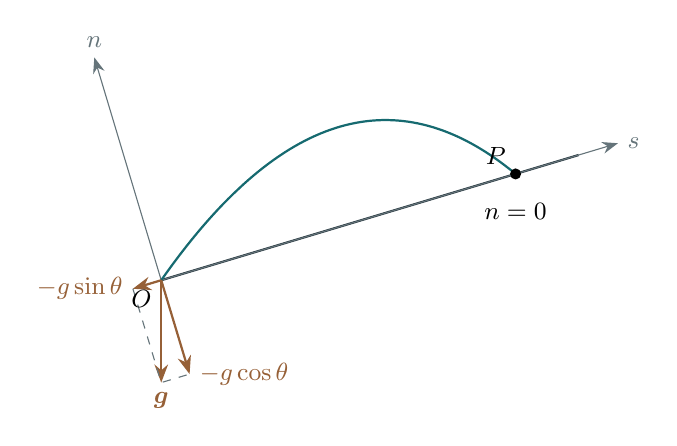
\begin{tikzpicture}

\draw[object] (0,0)--(5.3,1.59);
\draw[axis] (-.3,-.09)--(5.8,1.74) node[right] {$s$};
\draw[axis] (.09,-.3)--(-.85,2.83) node[above] {$n$};
\draw[traj,domain=0:4.5,samples=70] plot(\x,{(10/7)*\x-((10/7)-.3)*\x^2/4.5});
\fill (4.5,1.35) circle(2pt);\node[above left] at (4.5,1.35) {$P$};\node[below] at (4.5,1.10) {$n=0$};
\draw[force] (0,0)--(0,-1.3) node[below] {$\vect g$};
\draw[force] (0,0)--(-.36,-.108) node[left] {$-g\sin\theta$};
\draw[force] (0,0)--(.36,-1.192) node[right] {$-g\cos\theta$};
\draw[guide] (-.36,-.108)--(0,-1.3)--(.36,-1.192);
\node[below left] at (0,0) {$O$};

\end{tikzpicture}
\figcaption{解图 1.4B\quad 沿坡与垂直坡面建立坐标，飞行终点的条件变为 $n=0$。}
\end{minipage}\end{center}
\[
s=v_0\cos\alpha\,t-\frac12g\sin\theta\,t^2,
\qquad n=v_0\sin\alpha\,t-\frac12g\cos\theta\,t^2.
\]
由第二次 $n=0$ 得到同一 $t_f$；将它代入 $s$，展开后为
\[
R=\frac{2v_0^2\sin\alpha}{g\cos^2\theta}
(\cos\alpha\cos\theta-\sin\alpha\sin\theta),
\]
即上面的射程式。
\subsubsection*{求最优角}
用积化和差公式，
\[
2\sin\alpha\cos(\theta+\alpha)
=\sin(\theta+2\alpha)-\sin\theta.
\]
因而
\[
R(\alpha)=\frac{v_0^2}{g\cos^2\theta}
[\sin(\theta+2\alpha)-\sin\theta].
\]
在题设区间内，$\theta+2\alpha$ 可取 $\pi/2$；正弦的最大值为一，故
\[
\boxed{\alpha_*=\frac\pi4-\frac\theta2},\qquad
\boxed{R_{\max}=\frac{v_0^2(1-\sin\theta)}{g\cos^2\theta}
=\frac{v_0^2}{g(1+\sin\theta)}}.
\]
水平仰角则为 $\beta_* =\pi/4+\theta/2$。$\theta=0$ 时恢复水平地面的 $45^\circ$ 与 $v_0^2/g$；$\theta\to\pi/2^-$ 时沿坡最大射程趋于 $v_0^2/(2g)$，水平射程趋于零。
\subsubsection*{对落点横坐标求导的另一方法}
固定坡角时，解图1.4A中的$x_f$与沿坡射程$R$只相差正因子$\cos\theta$，
所以两者在同一发射角处取最大值。将第二交点写为
\[
x_f=\frac{v_0^2}{g}
\left[\sin2\beta-2\tan\theta\cos^2\beta\right],
\qquad \beta=\theta+\alpha,
\]
对$\alpha$求导时$\dd\beta/\dd\alpha=1$，从而
\[
\frac{\dd x_f}{\dd\alpha}
=\frac{2v_0^2}{g}
[\cos2\beta+\tan\theta\sin2\beta]
=\frac{2v_0^2}{g\cos\theta}\cos(2\beta-\theta).
\]
允许区间内的零点为$2\beta-\theta=\pi/2$，即
$\alpha=\pi/4-\theta/2$；从小仰角逐渐抬高炮口时，$x_f$先增加，越过这个角度后减小。
当$\alpha$趋近区间两端时，第二交点都回到炮口，射程趋于零，
这个内部驻点给出最大射程。求导还能说明从小仰角继续抬高时，落点怎样先远离炮口再返回。


\Needspace{5\baselineskip}

\pdfbookmark[3]{关键洞察}{q4-h5}

\subsection*{关键洞察}

固定坡角后，决定射程变化的是$\sin(2\alpha+\theta)$。最远时$2\alpha+\theta=\pi/2$，因而炮口与坡面的夹角为$\pi/4-\theta/2$，与水平线的夹角为$\pi/4+\theta/2$。变图1.4V4画出两个角随坡度的变化。坡面变陡时，炮口向竖直方向抬高，同时与坡面更加接近。

\Needspace{5\baselineskip}

\pdfbookmark[3]{易错点}{q4-h6}

\subsection*{易错点}

\begin{itemize}
\item 解图1.4A的水平、竖直分量使用$\beta$，解图1.4B的沿坡、法向分量使用$\alpha$。
\item 轨迹和坡线在炮口$O$已有交点。用$t>0$对应的交点$P$求射程。
\item 将沿坡长度投影到$x$轴得到$x_f$，换回沿坡长度时用
\[
R=\frac{x_f}{\cos\theta}.
\]
\item 对$\alpha$求极值前，先把$2\sin\alpha\cos(\theta+\alpha)$化成$\sin(\theta+2\alpha)-\sin\theta$。当$\theta=0$时，最优角为$45^\circ$，射程为$v_0^2/g$。
\end{itemize}

\Needspace{5\baselineskip}

\pdfbookmark[3]{课堂讲解建议}{q4-h7}

\subsection*{课堂讲解建议}

在图1.4中分别描出水平线、坡线和炮口方向，请学生沿三条线标出$\theta,\alpha,\theta+\alpha$。让学生先回答“坡面上第一个交点在哪里”，再把正飞行时间代回位置式。此时请学生在图中从$P$向下作垂线，说明$x_f$与$R$的比例。

板书保留$2\sin\alpha\cos(\theta+\alpha)=\sin(\theta+2\alpha)-\sin\theta$。从正弦最大值读出最优角后，在解图1.4B改用法向坐标求飞行时间。问“改求最远的水平投影，炮口要再转动吗”，用变图1.4V2中的$OH=OP\cos\theta$解释同一落点使两个距离同时最大。最后让学生用变图1.4V5比较水平坡面和近竖直坡面。

\Needspace{5\baselineskip}

\pdfbookmark[3]{变式训练}{q4-h8}

\subsection*{变式训练}

\begin{enumerate}
\item \textbf{向右下倾的山坡。}山坡角满足$-\pi/2<\theta<0$，炮弹向右并从坡面上方射出。求沿坡最远落点对应的仰角和射程。

变图1.4V1从向右的水平线量$\beta$，从坡面量$\alpha=\beta-\theta$。向右发射且初速指向坡面上方给出$\theta<\beta<\pi/2$。将$y=x\tan\theta$代入抛体坐标，取$t>0$的一根，得$t_f=2v_0\sin\alpha/(g\cos\theta)$。由于$\beta<\pi/2$，落点的水平坐标为正，沿下坡方向的射程为
\[
R=\frac{x_f}{\cos\theta}
=\frac{v_0^2}{g\cos^2\theta}[\sin(2\beta-\theta)-\sin\theta].
\]
当$2\beta-\theta=\pi/2$时取最大值。于是$\alpha_*=\pi/4-\theta/2>\pi/4$，而$\beta_*=\pi/4+\theta/2<\pi/4$。最大射程为$v_0^2/[g(1+\sin\theta)]$。
\begin{center}\begin{minipage}{.98\linewidth}\centering
\begin{tikzpicture}
\draw[axis] (-.3,0)--(6.1,0) node[right] {$x$};
\draw[object] (0,0)--(5.7,-1.9) node[right] {坡面};
\draw[traj,domain=0:5,samples=70] plot(\x,{.72*\x-(.72+1/3)*\x^2/5});
\draw[motion] (0,0)--(1.5,1.08) node[above] {$\vect v_0$};
\draw (1.05,-.35) arc[start angle=-18.435,end angle=0,radius=1.1068];
\node at (1.46,-.18) {$|\theta|$};
\draw (.665,-.222) arc[start angle=-18.435,end angle=35.75,radius=.701];
\node at (.88,.32) {$\alpha$};
\fill (5,-1.6667) circle(1.6pt) node[below left] {$P$};
\node[below left] at (0,0) {$O$};
\end{tikzpicture}
\figcaption{变图1.4V1\quad 坡面低于发射点，炮弹在右侧与坡面相交}
\end{minipage}\end{center}

\item \textbf{最大水平射程。}固定上坡坡角，改求$x_f$的最大值及相应角度。

图1.4V2中$OP$是沿坡射程，$P$的垂直投影为$H$，故$OH=x_f=R\cos\theta$。随发射角变化，$P$在同一条坡线上移动，比例$OH/OP=\cos\theta$固定且为正。于是两段距离在同一发射角$\alpha_*=\pi/4-\theta/2$处最长，得到
\[
x_{\max}=R_{\max}\cos\theta
=\frac{v_0^2\cos\theta}{g(1+\sin\theta)}.
\]
\begin{center}\begin{minipage}{.98\linewidth}\centering
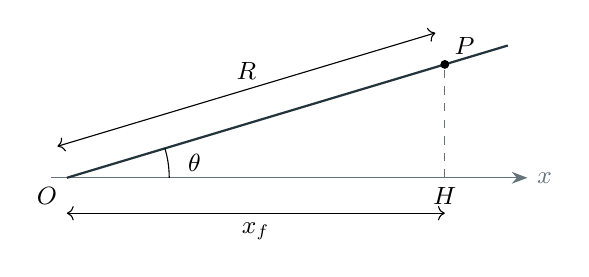
\begin{tikzpicture}
\draw[axis] (-.2,0)--(5.85,0) node[right] {$x$};
\draw[object] (0,0)--(5.6,1.68);
\draw[guide] (4.8,0)--(4.8,1.44);
\draw[thin,<->] (0,-.45)--(4.8,-.45) node[midway,below] {$x_f$};
\draw[thin,<->] (-.12,.4)--(4.68,1.84) node[midway,above] {$R$};
\fill (4.8,1.44) circle(1.6pt) node[above right] {$P$};
\node[below] at (4.8,0) {$H$};
\node[below left] at (0,0) {$O$};
\draw (1.3,0) arc(0:16.699:1.3);\node at (1.62,.19) {$\theta$};
\end{tikzpicture}
\figcaption{变图1.4V2\quad 沿坡射程在水平方向上的投影}
\end{minipage}\end{center}

\item \textbf{沿坡坐标中的最远落点。}在$s,n$坐标内直接求最优角。图1.4V3把初速度与重力分别投影在这两个方向上。落地时法向位移再次为零，因此
\[
n(t)=v_0\sin\alpha\,t-\tfrac12g\cos\theta\,t^2,
\qquad
t_f=\frac{2v_0\sin\alpha}{g\cos\theta}.
\]
将此时刻代入$s(t)=v_0\cos\alpha\,t-g\sin\theta\,t^2/2$，得到两项：
\[
R=\frac{2v_0^2\sin\alpha\cos\alpha}{g\cos\theta}
-\frac{2v_0^2\sin^2\alpha\sin\theta}{g\cos^2\theta}.
\]
提取公因子后，括号内是$\cos\alpha\cos\theta-\sin\alpha\sin\theta$，即$\cos(\theta+\alpha)$。于是
\[
R=\frac{v_0^2}{g\cos^2\theta}[\sin(2\alpha+\theta)-\sin\theta].
\]
令正弦为1，读得$\alpha_*=\pi/4-\theta/2$。
\begin{center}\begin{minipage}{.98\linewidth}\centering
\begin{tikzpicture}
\draw[axis] (-1,0)--(5.7,0) node[right] {$s$};
\draw[axis] (0,-1.6)--(0,2.5) node[above] {$n$};
\draw[motion] (0,0)--(2.5,1.5) node[right] {$\vect v_0$};
\draw[guide] (0,1.5)--(2.5,1.5)--(2.5,0);
\node[left] at (0,1.5) {$v_0\sin\alpha$};
\node[below] at (2.5,0) {$v_0\cos\alpha$};
\draw[force] (0,0)--(-.45,-1.5) node[below left] {$\vect g$};
\draw[guide] (-.45,0)--(-.45,-1.5)--(0,-1.5);
\node[above left] at (-.45,0) {$-g\sin\theta$};
\node[right] at (0,-1.5) {$-g\cos\theta$};
\draw (.78,0) arc(0:30.964:.78);\node at (1.06,.22) {$\alpha$};
\end{tikzpicture}
\figcaption{变图1.4V3\quad 以$s,n$为直角坐标绘制速度与重力的两个分量}
\end{minipage}\end{center}

\item \textbf{改变坡角时的最优发射方向。}保持$v_0$不变，求最优相对角、最优水平角与最大射程随坡角的变化。

由$\beta_*=\theta+\alpha_*$，图1.4V4中两角相对于$\theta$的斜率分别为$-1/2$与$1/2$。由射程式求导，
\[
\frac{\dd\alpha_*}{\dd\theta}=-\frac12,\qquad
\frac{\dd\beta_*}{\dd\theta}=\frac12,\qquad
\frac{\dd R_{\max}}{\dd\theta}
=-\frac{v_0^2\cos\theta}{g(1+\sin\theta)^2}.
\]
坡越陡，最优炮口越靠近竖直方向，炮口与坡面的夹角越小。最大射程也随坡角增大而缩短。
\begin{center}\begin{minipage}{.98\linewidth}\centering
\begin{tikzpicture}
\draw[axis] (0,0)--(5.65,0) node[right] {$\theta$};
\draw[axis] (0,0)--(0,3.1) node[above] {角度};
\draw[traj] (0,1.3)--(5,2.6) node[right] {$\beta_*$};
\draw[thick,dashed,warm] (0,1.3)--(5,0) node[above right] {$\alpha_*$};
\draw[guide] (0,2.6)--(5,2.6)--(5,0);
\node[left] at (0,1.3) {$\pi/4$};\node[left] at (0,2.6) {$\pi/2$};
\node[below] at (5,0) {$\pi/2$};
\end{tikzpicture}
\figcaption{变图1.4V4\quad 两个最优角在水平坡面相同，随坡角向相反方向变化}
\end{minipage}\end{center}

\item \textbf{水平坡与陡坡极限。}求最优发射时$R_{\max}$及$x_{\max}$在$\theta=0$和$\theta\to\pi/2^-$的值，并说明图中的两个终值。

把式中的$\cos^2\theta$写为$(1-\sin\theta)(1+\sin\theta)$，约去$1-\sin\theta$后再取极限：
\[
\frac{gR_{\max}}{v_0^2}=\frac1{1+\sin\theta},\qquad
\frac{gx_{\max}}{v_0^2}=\frac{\cos\theta}{1+\sin\theta}.
\]
图1.4V5在$\theta=0$处两条线均从1出发，对应$45^\circ$发射与$v_0^2/g$的射程。随着坡面趋近竖直，$\alpha_*\to0$、$\beta_*\to\pi/2$。沿坡射程趋于$v_0^2/(2g)$，水平投影则趋零。
\begin{center}\begin{minipage}{.98\linewidth}\centering
\begin{tikzpicture}
\draw[axis] (0,0)--(6.15,0) node[right] {$\theta$};
\draw[axis] (0,0)--(0,3.15) node[above] {距离比};
\draw[traj,domain=0:90,samples=80] plot({\x/18},{2.55/(1+sin(\x))});
\draw[thick,dashed,warm,domain=0:90,samples=80] plot({\x/18},{2.55*cos(\x)/(1+sin(\x))});
\draw[guide] (0,1.275)--(5,1.275)--(5,0);
\node[left] at (0,1.275) {$1/2$};\node[left] at (0,2.55) {$1$};
\node[below] at (5,0) {$\pi/2$};
\node[right] at (5,1.275) {$gR_{\max}/v_0^2$};
\node[right,warm] at (3.12,.78) {$gx_{\max}/v_0^2$};
\end{tikzpicture}
\figcaption{变图1.4V5\quad 沿坡距离与它的水平投影在陡坡极限取不同的值}
\end{minipage}\end{center}
\end{enumerate}

\clearpage

\pdfbookmark[2]{第 5 题 等射程抛体的飞行时间乘积}{q5}

\section*{第 5 题\quad 等射程抛体的飞行时间乘积}

\tagline{M-01-05}

两质点从同一水平地面上的同一点，以相同速率 $v_0$、不同仰角 $\alpha_1$ 和 $\alpha_2$ 抛出，且 $0<\alpha_1,\alpha_2<\pi/2$。两质点均落回该水平地面，空气阻力忽略。

若两次抛射的射程同为 $R$，证明两次飞行时间满足
\[
T_1T_2=\frac{2R}{g}.
\]

\begin{center}
\begin{tikzpicture}[x=1cm,y=1cm]
\draw[axis] (-.35,0)--(6.5,0) node[right] {$x$};\draw[axis] (0,-.2)--(0,3.5) node[above] {$y$};
\draw[traj,domain=0:6,samples=70] plot (\x,{1.73205*\x*(1-\x/6)});
\draw[traj,dashed,domain=0:6,samples=70] plot (\x,{.57735*\x*(1-\x/6)});
\draw[motion] (0,0)--(.6,1.039);\draw[motion] (0,0)--(1.039,.6);
\draw (.7,0) arc(0:30:.7);\node at (1,.22) {$\alpha_1$};
\draw (1.0,0) arc(0:60:1);\node at (1.05,1.05) {$\alpha_2$};
\node[color=accent] at (4.2,2.7) {高轨迹};\node[color=accent] at (4.5,.95) {低轨迹};
\fill (6,0) circle (1.8pt);\node[below] at (6,-.05) {$R$};\node[below left] at (0,0) {$O$};
\end{tikzpicture}
\figcaption{图 1.5\quad 同初速、同射程的两条不同轨迹。}
\end{center}

\Needspace{5\baselineskip}

\pdfbookmark[3]{题型定位}{q5-h0}

\subsection*{题型定位}

比较同速率斜抛的两条等射程轨迹。共同射程确定一对互余发射角，由两竖直初速度的乘积求时间积，再把时间与轨迹最高点的高度联系起来。

\Needspace{5\baselineskip}

\pdfbookmark[3]{知识点}{q5-h1}

\subsection*{知识点}

水平匀速与竖直匀变速共同给出 $R=v_0^2\sin2\alpha/g$ 和 $T=2v_0\sin\alpha/g$。射程曲线关于 $45^\circ$ 对称，利用差化积可解出等射程的两个角。最高点位于 $x=R/2$，其高度为 $H_i=gT_i^2/8$。


\Needspace{5\baselineskip}

\pdfbookmark[3]{物理图像}{q5-h2}

\subsection*{物理图像}

题图1.5中，低角度轨迹的水平初速度大、竖直初速度小，飞行时间短。解图1.5A把两次等射程画成一条水平线，与射程曲线有两个交点。两条轨迹的顶点沿同一竖线对齐，高轨迹的顶点到地面距离较大，下落所需时间也较长。

\Needspace{5\baselineskip}

\pdfbookmark[3]{解题入口}{q5-h3}

\subsection*{解题入口}

先由 $y=0$ 取落地的正时间根，再乘水平速度求射程。比较两次射程并差化积，在两个角均为锐角且彼此不同的条件下得到 $\alpha_1+\alpha_2=\pi/2$。时间式相乘后把 $\sin\alpha_2$ 换成 $\cos\alpha_1$，即可用 $\sin2\alpha_1$ 消去角度。

\Needspace{5\baselineskip}

\pdfbookmark[3]{标准解法}{q5-h4}

\subsection*{标准解法}

题图 1.5 的两条轨迹从同一点出发并落到同一水平地面。低角度轨迹的水平速度较大，高角度轨迹的竖直初速度较大；先由落地条件分别求时间和射程。
\subsubsection*{单次抛射的时间与射程}
对仰角为 $\alpha$ 的一次运动，
\[
x=v_0\cos\alpha\,t,\qquad
y=v_0\sin\alpha\,t-\frac12gt^2.
\]
落回地面时 $y=0$。舍去发射根 $t=0$ 后，
\[
T=\frac{2v_0\sin\alpha}{g},\qquad
R=v_0\cos\alpha\,T=\frac{v_0^2}{g}\sin2\alpha.
\]
\subsubsection*{等射程的两角互余}
初速相同、射程相同，故 $\sin2\alpha_1=\sin2\alpha_2$。将差化为乘积，
\[
2\cos(\alpha_1+\alpha_2)\sin(\alpha_1-\alpha_2)=0.
\]
两角均在 $(0,\pi/2)$ 且不同，所以 $\sin(\alpha_1-\alpha_2)\ne0$，只能有
\[
\boxed{\alpha_1+\alpha_2=\frac\pi2}.
\]
\begin{center}\begin{minipage}{\linewidth}\centering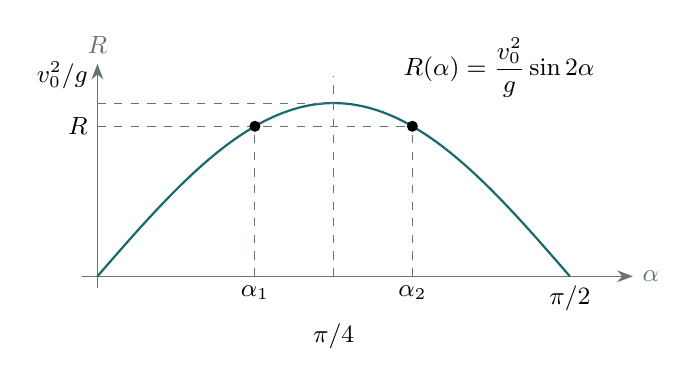
\begin{tikzpicture}

\draw[axis] (-.2,0)--(6.8,0) node[right] {$\alpha$};\draw[axis] (0,-.15)--(0,2.7) node[above] {$R$};
\draw[traj,domain=0:6,samples=90] plot(\x,{2.2*sin(30*\x)});
\draw[guide] (0,{2.2*sin(60)})--(4,{2.2*sin(60)});\node[left] at (0,{2.2*sin(60)}) {$R$};
\draw[guide] (0,2.2)--(3,2.2);\node[above left,yshift=1.5pt] at (0,2.2) {$v_0^2/g$};
\draw[guide] (2,0)--(2,{2.2*sin(60)});\draw[guide] (4,0)--(4,{2.2*sin(60)});
\fill (2,{2.2*sin(60)}) circle(2pt);\fill (4,{2.2*sin(60)}) circle(2pt);
\node[below] at (2,0) {$\alpha_1$};\node[below] at (4,0) {$\alpha_2$};\node[below] at (6,0) {$\pi/2$};
\draw[guide] (3,0)--(3,2.55);\node[below] at (3,-.48) {$\pi/4$};
\node at (5.1,2.65) {$R(\alpha)=\dfrac{v_0^2}{g}\sin2\alpha$};

\end{tikzpicture}
\figcaption{解图 1.5A\quad 射程曲线关于 $\alpha=\pi/4$ 对称；同一射程的两个不同仰角互余。}
\end{minipage}\end{center}
解图 1.5A 中，两条竖虚线从同一射程水平线落到横轴，读得一低一高的两个角。它们到 $45^\circ$ 的距离相同。射程升至 $v_0^2/g$ 时，两交点合为顶点，对应唯一的 $45^\circ$ 发射角。
\subsubsection*{求飞行时间乘积}
分别写出两次飞行时间并相乘，
\[
T_1T_2=\frac{4v_0^2}{g^2}\sin\alpha_1\sin\alpha_2
=\frac{4v_0^2}{g^2}\sin\alpha_1\cos\alpha_1
=\frac{2v_0^2}{g^2}\sin2\alpha_1.
\]
由 $R=v_0^2\sin2\alpha_1/g$，得到
\[
\boxed{T_1T_2=\frac{2R}{g}}.
\]
从时间式看，低角度的竖直初速度较小，所以先回到地面。两次飞行时间的乘积由共同射程确定。$R/g$ 的量纲是时间平方。等高落地使两次时间都等于各自竖直初速度的 $2/g$ 倍，互余角又让这两个竖直分量恰好等于一次发射里的水平、竖直分量。
\subsubsection*{共同对称轴与两个顶点的高度}
消去时间并使用落点 $x=R,y=0$，任一轨迹可改写为
\[
y=x\tan\alpha\left(1-\frac{x}{R}\right).
\]
最高点都在 $x=R/2$，高度为 $H_i=R\tan\alpha_i/4$。因为两角互余，$\tan\alpha_1\tan\alpha_2=1$，所以
\[
H_1H_2=\frac{R^2}{16}.
\]
题图 1.5 中，两个最高点沿 $x=R/2$ 竖直对齐。每个质点从最高点以零竖直速度下落，经过 $T_i/2$ 到达地面，因此 $H_i=gT_i^2/8$。这给出 $T_1T_2=(8/g)\sqrt{H_1H_2}=2R/g$。读出两顶点的高度，还可用 $T_2/T_1=\sqrt{H_2/H_1}$ 比较飞行时间。

\Needspace{5\baselineskip}

\pdfbookmark[3]{关键洞察}{q5-h5}

\subsection*{关键洞察}

同速率时，互余变换交换水平、竖直初速度。两个速度分量的乘积相同，所以射程相同；分别把两竖直分量乘以 $2/g$，便得到两个飞行时间及其固定的乘积。

\Needspace{5\baselineskip}

\pdfbookmark[3]{易错点}{q5-h6}

\subsection*{易错点}

\begin{itemize}
\item 等射程方程有同角与互余两类解。题设指定不同角，差化积中的 $\sin(\alpha_1-\alpha_2)$ 非零。
\item 时间可由水平位移反算为 $T=R/(v_0\cos\alpha)$。分母取图中沿地面的速度分量。
\item $T=2v_0\sin\alpha/g$ 取自与发射点同高的落点。目标改在高度 $H$ 时，应把 $y=H$ 代入轨迹方程。
\end{itemize}

\Needspace{5\baselineskip}

\pdfbookmark[3]{课堂讲解建议}{q5-h7}

\subsection*{课堂讲解建议}

在解图1.5A上画一条低于顶点的水平线，问“右交点对应哪个角”。答为左交点角的余角，因为两点到 $45^\circ$ 的距离相等。随后让学生在题图标出两条轨迹的水平、竖直初速度，指出低轨迹先落地。把水平线抬到顶点，追问还有几个角可选，答为一个，即 $45^\circ$。最后问怎样由两顶点估计飞行时间比，利用从顶点到地面的自由落体得 $T_2/T_1=\sqrt{H_2/H_1}$。

\Needspace{5\baselineskip}

\pdfbookmark[3]{变式训练}{q5-h8}

\subsection*{变式训练}

\begin{enumerate}
\item 两次初速不同但射程同为 $R$，求飞行时间乘积，并判断它是否由 $R$ 唯一确定。把 $v_{iy}=gT_i/2$ 和 $v_{ix}=R/T_i$ 相除，得 $\tan\alpha_i=gT_i^2/(2R)$，故
\[
T_1T_2=\frac{2R}{g}\sqrt{\tan\alpha_1\tan\alpha_2}.
\]
变图1.5V1取 $30^\circ$ 和 $45^\circ$，分别用 $v_i^2=gR/\sin2\alpha_i$ 选初速。图中两条轨迹都到达 $x=R$，时间积却为 $(2R/g)3^{-1/4}$。当另给互余角条件时，两正切的乘积为一，时间积恢复为 $2R/g$。
\begin{center}\begin{minipage}{.98\linewidth}\centering
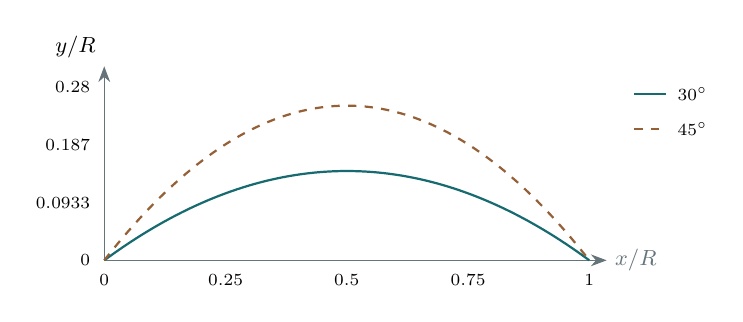
\begin{tikzpicture}[scale=.88,transform shape]
\draw[axis] (0,0.0000000)--(7.25,0.0000000) node[right] {$x/R$};
\draw[axis] (0.0000000,0)--(0.0000000,2.8);
\node[above left] at (0.0000000,2.8) {$y/R$};
\node[below,font=\scriptsize] at (0.0000000,-0.0800000) {$0$};
\node[below,font=\scriptsize] at (1.7500000,-0.0800000) {$0.25$};
\node[below,font=\scriptsize] at (3.5000000,-0.0800000) {$0.5$};
\node[below,font=\scriptsize] at (5.2500000,-0.0800000) {$0.75$};
\node[below,font=\scriptsize] at (7.0000000,-0.0800000) {$1$};
\node[left,font=\scriptsize] at (-0.0800000,0.0000000) {$0$};
\node[left,font=\scriptsize] at (-0.0800000,0.8333333) {$0.0933$};
\node[left,font=\scriptsize] at (-0.0800000,1.6666667) {$0.187$};
\node[left,font=\scriptsize] at (-0.0800000,2.5000000) {$0.28$};
\draw[thick,color=accent] plot coordinates {(0.0000000,0.0000000) (0.0583333,0.0425996) (0.1166667,0.0844833) (0.1750000,0.1256510) (0.2333333,0.1661028) (0.2916667,0.2058385) (0.3500000,0.2448584) (0.4083333,0.2831622) (0.4666667,0.3207501) (0.5250000,0.3576221) (0.5833333,0.3937781) (0.6416667,0.4292181) (0.7000000,0.4639422) (0.7583333,0.4979503) (0.8166667,0.5312424) (0.8750000,0.5638186) (0.9333333,0.5956788) (0.9916667,0.6268231) (1.0500000,0.6572514) (1.1083333,0.6869638) (1.1666667,0.7159602) (1.2250000,0.7442406) (1.2833333,0.7718050) (1.3416667,0.7986536) (1.4000000,0.8247861) (1.4583333,0.8502027) (1.5166667,0.8749033) (1.5750000,0.8988880) (1.6333333,0.9221567) (1.6916667,0.9447094) (1.7500000,0.9665462) (1.8083333,0.9876670) (1.8666667,1.0080719) (1.9250000,1.0277608) (1.9833333,1.0467337) (2.0416667,1.0649907) (2.1000000,1.0825318) (2.1583333,1.0993568) (2.2166667,1.1154659) (2.2750000,1.1308591) (2.3333333,1.1455362) (2.3916667,1.1594975) (2.4500000,1.1727427) (2.5083333,1.1852720) (2.5666667,1.1970854) (2.6250000,1.2081828) (2.6833333,1.2185642) (2.7416667,1.2282296) (2.8000000,1.2371791) (2.8583333,1.2454127) (2.9166667,1.2529303) (2.9750000,1.2597319) (3.0333333,1.2658176) (3.0916667,1.2711873) (3.1500000,1.2758410) (3.2083333,1.2797788) (3.2666667,1.2830006) (3.3250000,1.2855065) (3.3833333,1.2872964) (3.4416667,1.2883703) (3.5000000,1.2887283) (3.5583333,1.2883703) (3.6166667,1.2872964) (3.6750000,1.2855065) (3.7333333,1.2830006) (3.7916667,1.2797788) (3.8500000,1.2758410) (3.9083333,1.2711873) (3.9666667,1.2658176) (4.0250000,1.2597319) (4.0833333,1.2529303) (4.1416667,1.2454127) (4.2000000,1.2371791) (4.2583333,1.2282296) (4.3166667,1.2185642) (4.3750000,1.2081828) (4.4333333,1.1970854) (4.4916667,1.1852720) (4.5500000,1.1727427) (4.6083333,1.1594975) (4.6666667,1.1455362) (4.7250000,1.1308591) (4.7833333,1.1154659) (4.8416667,1.0993568) (4.9000000,1.0825318) (4.9583333,1.0649907) (5.0166667,1.0467337) (5.0750000,1.0277608) (5.1333333,1.0080719) (5.1916667,0.9876670) (5.2500000,0.9665462) (5.3083333,0.9447094) (5.3666667,0.9221567) (5.4250000,0.8988880) (5.4833333,0.8749033) (5.5416667,0.8502027) (5.6000000,0.8247861) (5.6583333,0.7986536) (5.7166667,0.7718050) (5.7750000,0.7442406) (5.8333333,0.7159602) (5.8916667,0.6869638) (5.9500000,0.6572514) (6.0083333,0.6268231) (6.0666667,0.5956788) (6.1250000,0.5638186) (6.1833333,0.5312424) (6.2416667,0.4979503) (6.3000000,0.4639422) (6.3583333,0.4292181) (6.4166667,0.3937781) (6.4750000,0.3576221) (6.5333333,0.3207501) (6.5916667,0.2831622) (6.6500000,0.2448584) (6.7083333,0.2058385) (6.7666667,0.1661028) (6.8250000,0.1256510) (6.8833333,0.0844833) (6.9416667,0.0425996) (7.0000000,0.0000000)};
\draw[thick,color=accent] (7.65,2.4)--(8.1,2.4);\node[right,font=\scriptsize] at (8.15,2.4) {$30^\circ$};
\draw[thick,dashed,color=warm] plot coordinates {(0.0000000,0.0000000) (0.0583333,0.0737847) (0.1166667,0.1463294) (0.1750000,0.2176339) (0.2333333,0.2876984) (0.2916667,0.3565228) (0.3500000,0.4241071) (0.4083333,0.4904514) (0.4666667,0.5555556) (0.5250000,0.6194196) (0.5833333,0.6820437) (0.6416667,0.7434276) (0.7000000,0.8035714) (0.7583333,0.8624752) (0.8166667,0.9201389) (0.8750000,0.9765625) (0.9333333,1.0317460) (0.9916667,1.0856895) (1.0500000,1.1383929) (1.1083333,1.1898562) (1.1666667,1.2400794) (1.2250000,1.2890625) (1.2833333,1.3368056) (1.3416667,1.3833085) (1.4000000,1.4285714) (1.4583333,1.4725942) (1.5166667,1.5153770) (1.5750000,1.5569196) (1.6333333,1.5972222) (1.6916667,1.6362847) (1.7500000,1.6741071) (1.8083333,1.7106895) (1.8666667,1.7460317) (1.9250000,1.7801339) (1.9833333,1.8129960) (2.0416667,1.8446181) (2.1000000,1.8750000) (2.1583333,1.9041419) (2.2166667,1.9320437) (2.2750000,1.9587054) (2.3333333,1.9841270) (2.3916667,2.0083085) (2.4500000,2.0312500) (2.5083333,2.0529514) (2.5666667,2.0734127) (2.6250000,2.0926339) (2.6833333,2.1106151) (2.7416667,2.1273562) (2.8000000,2.1428571) (2.8583333,2.1571181) (2.9166667,2.1701389) (2.9750000,2.1819196) (3.0333333,2.1924603) (3.0916667,2.2017609) (3.1500000,2.2098214) (3.2083333,2.2166419) (3.2666667,2.2222222) (3.3250000,2.2265625) (3.3833333,2.2296627) (3.4416667,2.2315228) (3.5000000,2.2321429) (3.5583333,2.2315228) (3.6166667,2.2296627) (3.6750000,2.2265625) (3.7333333,2.2222222) (3.7916667,2.2166419) (3.8500000,2.2098214) (3.9083333,2.2017609) (3.9666667,2.1924603) (4.0250000,2.1819196) (4.0833333,2.1701389) (4.1416667,2.1571181) (4.2000000,2.1428571) (4.2583333,2.1273562) (4.3166667,2.1106151) (4.3750000,2.0926339) (4.4333333,2.0734127) (4.4916667,2.0529514) (4.5500000,2.0312500) (4.6083333,2.0083085) (4.6666667,1.9841270) (4.7250000,1.9587054) (4.7833333,1.9320437) (4.8416667,1.9041419) (4.9000000,1.8750000) (4.9583333,1.8446181) (5.0166667,1.8129960) (5.0750000,1.7801339) (5.1333333,1.7460317) (5.1916667,1.7106895) (5.2500000,1.6741071) (5.3083333,1.6362847) (5.3666667,1.5972222) (5.4250000,1.5569196) (5.4833333,1.5153770) (5.5416667,1.4725942) (5.6000000,1.4285714) (5.6583333,1.3833085) (5.7166667,1.3368056) (5.7750000,1.2890625) (5.8333333,1.2400794) (5.8916667,1.1898562) (5.9500000,1.1383929) (6.0083333,1.0856895) (6.0666667,1.0317460) (6.1250000,0.9765625) (6.1833333,0.9201389) (6.2416667,0.8624752) (6.3000000,0.8035714) (6.3583333,0.7434276) (6.4166667,0.6820437) (6.4750000,0.6194196) (6.5333333,0.5555556) (6.5916667,0.4904514) (6.6500000,0.4241071) (6.7083333,0.3565228) (6.7666667,0.2876984) (6.8250000,0.2176339) (6.8833333,0.1463294) (6.9416667,0.0737847) (7.0000000,0.0000000)};
\draw[thick,dashed,color=warm] (7.65,1.9)--(8.1,1.9);\node[right,font=\scriptsize] at (8.15,1.9) {$45^\circ$};
\end{tikzpicture}
\figcaption{变图1.5V1\quad 不同初速、相同射程的两个实例。}
\end{minipage}\end{center}
\item 同速率 $v_0$ 抛向 $(R,H)$，求两发射角的关系。置 $p=\tan\alpha$、$A=gR^2/(2v_0^2)>0$，通过目标需满足 $Ap^2-Rp+(A+H)=0$。两个不同锐角对应判别式 $R^2-4A(A+H)>0$ 且两根为正。由韦达定理，
\[
p_1p_2=1+\frac{2v_0^2H}{gR^2},\qquad T_i=\frac{R\sqrt{1+p_i^2}}{v_0}>0.
\]
变图1.5V2取 $H=0.4R,A=0.25R$，两条实轨迹通过同一点，正切乘积为2.6。互余所需的乘积一对应 $H=0$。
\begin{center}\begin{minipage}{.98\linewidth}\centering
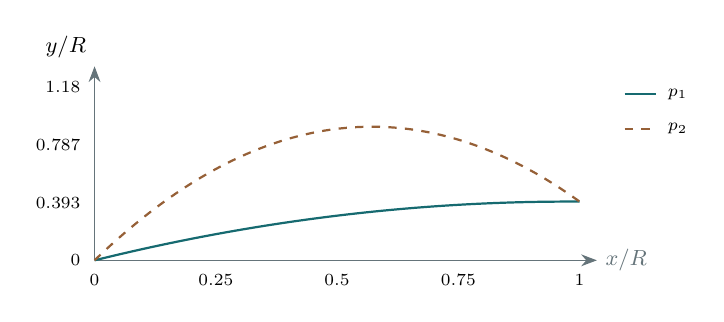
\begin{tikzpicture}[scale=.88,transform shape]
\draw[axis] (0,0.0000000)--(7.25,0.0000000) node[right] {$x/R$};
\draw[axis] (0.0000000,0)--(0.0000000,2.8);
\node[above left] at (0.0000000,2.8) {$y/R$};
\node[below,font=\scriptsize] at (0.0000000,-0.0800000) {$0$};
\node[below,font=\scriptsize] at (1.7500000,-0.0800000) {$0.25$};
\node[below,font=\scriptsize] at (3.5000000,-0.0800000) {$0.5$};
\node[below,font=\scriptsize] at (5.2500000,-0.0800000) {$0.75$};
\node[below,font=\scriptsize] at (7.0000000,-0.0800000) {$1$};
\node[left,font=\scriptsize] at (-0.0800000,0.0000000) {$0$};
\node[left,font=\scriptsize] at (-0.0800000,0.8333333) {$0.393$};
\node[left,font=\scriptsize] at (-0.0800000,1.6666667) {$0.787$};
\node[left,font=\scriptsize] at (-0.0800000,2.5000000) {$1.18$};
\draw[thick,color=accent] plot coordinates {(0.0000000,0.0000000) (0.0583333,0.0143593) (0.1166667,0.0285960) (0.1750000,0.0427100) (0.2333333,0.0567014) (0.2916667,0.0705701) (0.3500000,0.0843162) (0.4083333,0.0979396) (0.4666667,0.1114405) (0.5250000,0.1248186) (0.5833333,0.1380742) (0.6416667,0.1512070) (0.7000000,0.1642173) (0.7583333,0.1771049) (0.8166667,0.1898699) (0.8750000,0.2025122) (0.9333333,0.2150319) (0.9916667,0.2274289) (1.0500000,0.2397033) (1.1083333,0.2518551) (1.1666667,0.2638842) (1.2250000,0.2757907) (1.2833333,0.2875745) (1.3416667,0.2992357) (1.4000000,0.3107743) (1.4583333,0.3221902) (1.5166667,0.3334834) (1.5750000,0.3446541) (1.6333333,0.3557021) (1.6916667,0.3666274) (1.7500000,0.3774301) (1.8083333,0.3881102) (1.8666667,0.3986676) (1.9250000,0.4091024) (1.9833333,0.4194145) (2.0416667,0.4296040) (2.1000000,0.4396709) (2.1583333,0.4496151) (2.2166667,0.4594367) (2.2750000,0.4691356) (2.3333333,0.4787119) (2.3916667,0.4881655) (2.4500000,0.4974965) (2.5083333,0.5067049) (2.5666667,0.5157906) (2.6250000,0.5247537) (2.6833333,0.5335942) (2.7416667,0.5423120) (2.8000000,0.5509071) (2.8583333,0.5593797) (2.9166667,0.5677295) (2.9750000,0.5759568) (3.0333333,0.5840614) (3.0916667,0.5920433) (3.1500000,0.5999026) (3.2083333,0.6076393) (3.2666667,0.6152534) (3.3250000,0.6227447) (3.3833333,0.6301135) (3.4416667,0.6373596) (3.5000000,0.6444831) (3.5583333,0.6514839) (3.6166667,0.6583621) (3.6750000,0.6651176) (3.7333333,0.6717505) (3.7916667,0.6782608) (3.8500000,0.6846484) (3.9083333,0.6909134) (3.9666667,0.6970557) (4.0250000,0.7030754) (4.0833333,0.7089725) (4.1416667,0.7147469) (4.2000000,0.7203987) (4.2583333,0.7259278) (4.3166667,0.7313343) (4.3750000,0.7366181) (4.4333333,0.7417793) (4.4916667,0.7468179) (4.5500000,0.7517338) (4.6083333,0.7565271) (4.6666667,0.7611978) (4.7250000,0.7657458) (4.7833333,0.7701711) (4.8416667,0.7744738) (4.9000000,0.7786539) (4.9583333,0.7827114) (5.0166667,0.7866461) (5.0750000,0.7904583) (5.1333333,0.7941478) (5.1916667,0.7977147) (5.2500000,0.8011589) (5.3083333,0.8044805) (5.3666667,0.8076795) (5.4250000,0.8107558) (5.4833333,0.8137094) (5.5416667,0.8165404) (5.6000000,0.8192488) (5.6583333,0.8218346) (5.7166667,0.8242977) (5.7750000,0.8266381) (5.8333333,0.8288559) (5.8916667,0.8309511) (5.9500000,0.8329237) (6.0083333,0.8347735) (6.0666667,0.8365008) (6.1250000,0.8381054) (6.1833333,0.8395874) (6.2416667,0.8409467) (6.3000000,0.8421834) (6.3583333,0.8432974) (6.4166667,0.8442888) (6.4750000,0.8451576) (6.5333333,0.8459037) (6.5916667,0.8465272) (6.6500000,0.8470281) (6.7083333,0.8474063) (6.7666667,0.8476618) (6.8250000,0.8477947) (6.8833333,0.8478050) (6.9416667,0.8476926) (7.0000000,0.8474576)};
\draw[thick,color=accent] (7.65,2.4)--(8.1,2.4);\node[right,font=\scriptsize] at (8.15,2.4) {$p_1$};
\draw[thick,dashed,color=warm] plot coordinates {(0.0000000,0.0000000) (0.0583333,0.0557914) (0.1166667,0.1107637) (0.1750000,0.1649171) (0.2333333,0.2182516) (0.2916667,0.2707670) (0.3500000,0.3224635) (0.4083333,0.3733410) (0.4666667,0.4233995) (0.5250000,0.4726390) (0.5833333,0.5210596) (0.6416667,0.5686611) (0.7000000,0.6154437) (0.7583333,0.6614073) (0.8166667,0.7065520) (0.8750000,0.7508776) (0.9333333,0.7943843) (0.9916667,0.8370720) (1.0500000,0.8789408) (1.1083333,0.9199905) (1.1666667,0.9602213) (1.2250000,0.9996331) (1.2833333,1.0382259) (1.3416667,1.0759997) (1.4000000,1.1129546) (1.4583333,1.1490904) (1.5166667,1.1844073) (1.5750000,1.2189053) (1.6333333,1.2525842) (1.6916667,1.2854442) (1.7500000,1.3174852) (1.8083333,1.3487072) (1.8666667,1.3791102) (1.9250000,1.4086942) (1.9833333,1.4374593) (2.0416667,1.4654054) (2.1000000,1.4925325) (2.1583333,1.5188407) (2.2166667,1.5443298) (2.2750000,1.5690000) (2.3333333,1.5928512) (2.3916667,1.6158834) (2.4500000,1.6380967) (2.5083333,1.6594909) (2.5666667,1.6800662) (2.6250000,1.6998225) (2.6833333,1.7187599) (2.7416667,1.7368782) (2.8000000,1.7541776) (2.8583333,1.7706580) (2.9166667,1.7863194) (2.9750000,1.8011619) (3.0333333,1.8151853) (3.0916667,1.8283898) (3.1500000,1.8407753) (3.2083333,1.8523418) (3.2666667,1.8630894) (3.3250000,1.8730180) (3.3833333,1.8821276) (3.4416667,1.8904182) (3.5000000,1.8978898) (3.5583333,1.9045425) (3.6166667,1.9103761) (3.6750000,1.9153908) (3.7333333,1.9195866) (3.7916667,1.9229633) (3.8500000,1.9255211) (3.9083333,1.9272599) (3.9666667,1.9281797) (4.0250000,1.9282805) (4.0833333,1.9275624) (4.1416667,1.9260252) (4.2000000,1.9236691) (4.2583333,1.9204940) (4.3166667,1.9165000) (4.3750000,1.9116869) (4.4333333,1.9060549) (4.4916667,1.8996039) (4.5500000,1.8923340) (4.6083333,1.8842450) (4.6666667,1.8753371) (4.7250000,1.8656102) (4.7833333,1.8550643) (4.8416667,1.8436994) (4.9000000,1.8315156) (4.9583333,1.8185128) (5.0166667,1.8046910) (5.0750000,1.7900502) (5.1333333,1.7745904) (5.1916667,1.7583117) (5.2500000,1.7412140) (5.3083333,1.7232973) (5.3666667,1.7045616) (5.4250000,1.6850070) (5.4833333,1.6646333) (5.5416667,1.6434407) (5.6000000,1.6214291) (5.6583333,1.5985986) (5.7166667,1.5749490) (5.7750000,1.5504805) (5.8333333,1.5251930) (5.8916667,1.4990865) (5.9500000,1.4721611) (6.0083333,1.4444167) (6.0666667,1.4158532) (6.1250000,1.3864709) (6.1833333,1.3562695) (6.2416667,1.3252491) (6.3000000,1.2934098) (6.3583333,1.2607515) (6.4166667,1.2272742) (6.4750000,1.1929780) (6.5333333,1.1578627) (6.5916667,1.1219285) (6.6500000,1.0851753) (6.7083333,1.0476032) (6.7666667,1.0092120) (6.8250000,0.9700019) (6.8833333,0.9299728) (6.9416667,0.8891247) (7.0000000,0.8474576)};
\draw[thick,dashed,color=warm] (7.65,1.9)--(8.1,1.9);\node[right,font=\scriptsize] at (8.15,1.9) {$p_2$};
\end{tikzpicture}
\figcaption{变图1.5V2\quad 固定初速时，两条曲线都通过目标 $(1,0.4)$。}
\end{minipage}\end{center}
\item 求两条等射程轨迹的最高点高度之和与积。由变图1.5V3，顶点均在 $x=R/2$，所以 $H_i=(R/4)\tan\alpha_i$。利用两角互余，得 $H_1H_2=R^2/16$。再用 $H_i=v_0^2\sin^2\alpha_i/(2g)$，得到
\[
H_1+H_2=\frac{v_0^2}{2g}(\sin^2\alpha_1+\cos^2\alpha_1)=\frac{v_0^2}{2g}.
\]
给定共同射程与初速后，也可把这两个高度作为以该和与积确定的二次方程两根。
\begin{center}\begin{minipage}{.98\linewidth}\centering
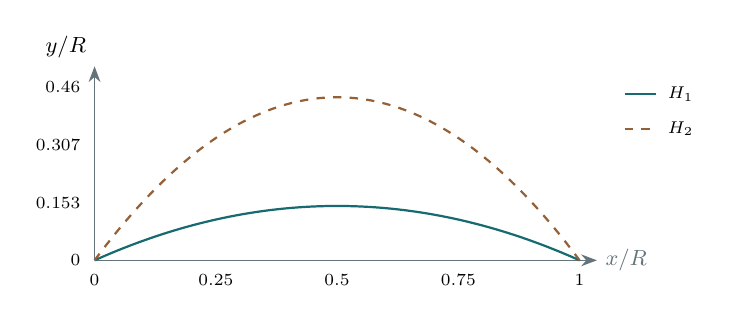
\begin{tikzpicture}[scale=.88,transform shape]
\draw[axis] (0,0.0000000)--(7.25,0.0000000) node[right] {$x/R$};
\draw[axis] (0.0000000,0)--(0.0000000,2.8);
\node[above left] at (0.0000000,2.8) {$y/R$};
\node[below,font=\scriptsize] at (0.0000000,-0.0800000) {$0$};
\node[below,font=\scriptsize] at (1.7500000,-0.0800000) {$0.25$};
\node[below,font=\scriptsize] at (3.5000000,-0.0800000) {$0.5$};
\node[below,font=\scriptsize] at (5.2500000,-0.0800000) {$0.75$};
\node[below,font=\scriptsize] at (7.0000000,-0.0800000) {$1$};
\node[left,font=\scriptsize] at (-0.0800000,0.0000000) {$0$};
\node[left,font=\scriptsize] at (-0.0800000,0.8333333) {$0.153$};
\node[left,font=\scriptsize] at (-0.0800000,1.6666667) {$0.307$};
\node[left,font=\scriptsize] at (-0.0800000,2.5000000) {$0.46$};
\draw[thick,color=accent] plot coordinates {(0.0000000,0.0000000) (0.0583333,0.0259302) (0.1166667,0.0514246) (0.1750000,0.0764832) (0.2333333,0.1011060) (0.2916667,0.1252930) (0.3500000,0.1490442) (0.4083333,0.1723596) (0.4666667,0.1952392) (0.5250000,0.2176830) (0.5833333,0.2396910) (0.6416667,0.2612632) (0.7000000,0.2823996) (0.7583333,0.3031002) (0.8166667,0.3233650) (0.8750000,0.3431939) (0.9333333,0.3625871) (0.9916667,0.3815445) (1.0500000,0.4000661) (1.1083333,0.4181519) (1.1666667,0.4358018) (1.2250000,0.4530160) (1.2833333,0.4697944) (1.3416667,0.4861369) (1.4000000,0.5020437) (1.4583333,0.5175147) (1.5166667,0.5325498) (1.5750000,0.5471492) (1.6333333,0.5613128) (1.6916667,0.5750405) (1.7500000,0.5883325) (1.8083333,0.6011886) (1.8666667,0.6136090) (1.9250000,0.6255935) (1.9833333,0.6371423) (2.0416667,0.6482552) (2.1000000,0.6589324) (2.1583333,0.6691737) (2.2166667,0.6789793) (2.2750000,0.6883490) (2.3333333,0.6972829) (2.3916667,0.7057811) (2.4500000,0.7138434) (2.5083333,0.7214699) (2.5666667,0.7286607) (2.6250000,0.7354156) (2.6833333,0.7417347) (2.7416667,0.7476180) (2.8000000,0.7530656) (2.8583333,0.7580773) (2.9166667,0.7626532) (2.9750000,0.7667933) (3.0333333,0.7704976) (3.0916667,0.7737662) (3.1500000,0.7765989) (3.2083333,0.7789958) (3.2666667,0.7809569) (3.3250000,0.7824822) (3.3833333,0.7835717) (3.4416667,0.7842254) (3.5000000,0.7844433) (3.5583333,0.7842254) (3.6166667,0.7835717) (3.6750000,0.7824822) (3.7333333,0.7809569) (3.7916667,0.7789958) (3.8500000,0.7765989) (3.9083333,0.7737662) (3.9666667,0.7704976) (4.0250000,0.7667933) (4.0833333,0.7626532) (4.1416667,0.7580773) (4.2000000,0.7530656) (4.2583333,0.7476180) (4.3166667,0.7417347) (4.3750000,0.7354156) (4.4333333,0.7286607) (4.4916667,0.7214699) (4.5500000,0.7138434) (4.6083333,0.7057811) (4.6666667,0.6972829) (4.7250000,0.6883490) (4.7833333,0.6789793) (4.8416667,0.6691737) (4.9000000,0.6589324) (4.9583333,0.6482552) (5.0166667,0.6371423) (5.0750000,0.6255935) (5.1333333,0.6136090) (5.1916667,0.6011886) (5.2500000,0.5883325) (5.3083333,0.5750405) (5.3666667,0.5613128) (5.4250000,0.5471492) (5.4833333,0.5325498) (5.5416667,0.5175147) (5.6000000,0.5020437) (5.6583333,0.4861369) (5.7166667,0.4697944) (5.7750000,0.4530160) (5.8333333,0.4358018) (5.8916667,0.4181519) (5.9500000,0.4000661) (6.0083333,0.3815445) (6.0666667,0.3625871) (6.1250000,0.3431939) (6.1833333,0.3233650) (6.2416667,0.3031002) (6.3000000,0.2823996) (6.3583333,0.2612632) (6.4166667,0.2396910) (6.4750000,0.2176830) (6.5333333,0.1952392) (6.5916667,0.1723596) (6.6500000,0.1490442) (6.7083333,0.1252930) (6.7666667,0.1011060) (6.8250000,0.0764832) (6.8833333,0.0514246) (6.9416667,0.0259302) (7.0000000,0.0000000)};
\draw[thick,color=accent] (7.65,2.4)--(8.1,2.4);\node[right,font=\scriptsize] at (8.15,2.4) {$H_1$};
\draw[thick,dashed,color=warm] plot coordinates {(0.0000000,0.0000000) (0.0583333,0.0777906) (0.1166667,0.1542738) (0.1750000,0.2294497) (0.2333333,0.3033181) (0.2916667,0.3758791) (0.3500000,0.4471327) (0.4083333,0.5170789) (0.4666667,0.5857177) (0.5250000,0.6530490) (0.5833333,0.7190730) (0.6416667,0.7837896) (0.7000000,0.8471988) (0.7583333,0.9093005) (0.8166667,0.9700949) (0.8750000,1.0295818) (0.9333333,1.0877614) (0.9916667,1.1446335) (1.0500000,1.2001982) (1.1083333,1.2544556) (1.1666667,1.3074055) (1.2250000,1.3590480) (1.2833333,1.4093831) (1.3416667,1.4584108) (1.4000000,1.5061311) (1.4583333,1.5525440) (1.5166667,1.5976495) (1.5750000,1.6414476) (1.6333333,1.6839383) (1.6916667,1.7251216) (1.7500000,1.7649974) (1.8083333,1.8035659) (1.8666667,1.8408269) (1.9250000,1.8767806) (1.9833333,1.9114268) (2.0416667,1.9447657) (2.1000000,1.9767971) (2.1583333,2.0075211) (2.2166667,2.0369378) (2.2750000,2.0650470) (2.3333333,2.0918488) (2.3916667,2.1173432) (2.4500000,2.1415302) (2.5083333,2.1644098) (2.5666667,2.1859820) (2.6250000,2.2062468) (2.6833333,2.2252042) (2.7416667,2.2428541) (2.8000000,2.2591967) (2.8583333,2.2742319) (2.9166667,2.2879596) (2.9750000,2.3003800) (3.0333333,2.3114929) (3.0916667,2.3212985) (3.1500000,2.3297966) (3.2083333,2.3369873) (3.2666667,2.3428707) (3.3250000,2.3474466) (3.3833333,2.3507151) (3.4416667,2.3526762) (3.5000000,2.3533299) (3.5583333,2.3526762) (3.6166667,2.3507151) (3.6750000,2.3474466) (3.7333333,2.3428707) (3.7916667,2.3369873) (3.8500000,2.3297966) (3.9083333,2.3212985) (3.9666667,2.3114929) (4.0250000,2.3003800) (4.0833333,2.2879596) (4.1416667,2.2742319) (4.2000000,2.2591967) (4.2583333,2.2428541) (4.3166667,2.2252042) (4.3750000,2.2062468) (4.4333333,2.1859820) (4.4916667,2.1644098) (4.5500000,2.1415302) (4.6083333,2.1173432) (4.6666667,2.0918488) (4.7250000,2.0650470) (4.7833333,2.0369378) (4.8416667,2.0075211) (4.9000000,1.9767971) (4.9583333,1.9447657) (5.0166667,1.9114268) (5.0750000,1.8767806) (5.1333333,1.8408269) (5.1916667,1.8035659) (5.2500000,1.7649974) (5.3083333,1.7251216) (5.3666667,1.6839383) (5.4250000,1.6414476) (5.4833333,1.5976495) (5.5416667,1.5525440) (5.6000000,1.5061311) (5.6583333,1.4584108) (5.7166667,1.4093831) (5.7750000,1.3590480) (5.8333333,1.3074055) (5.8916667,1.2544556) (5.9500000,1.2001982) (6.0083333,1.1446335) (6.0666667,1.0877614) (6.1250000,1.0295818) (6.1833333,0.9700949) (6.2416667,0.9093005) (6.3000000,0.8471988) (6.3583333,0.7837896) (6.4166667,0.7190730) (6.4750000,0.6530490) (6.5333333,0.5857177) (6.5916667,0.5170789) (6.6500000,0.4471327) (6.7083333,0.3758791) (6.7666667,0.3033181) (6.8250000,0.2294497) (6.8833333,0.1542738) (6.9416667,0.0777906) (7.0000000,0.0000000)};
\draw[thick,dashed,color=warm] (7.65,1.9)--(8.1,1.9);\node[right,font=\scriptsize] at (8.15,1.9) {$H_2$};
\end{tikzpicture}
\figcaption{变图1.5V3\quad 两个顶点都在 $x=R/2$。}
\end{minipage}\end{center}
\item 一个发射角为 $30^\circ$，求另一个角与各自的飞行时间。由互余得另一角为 $60^\circ$，因而 $R=\sqrt3v_0^2/(2g)$。在变图1.5V4的高度曲线上读出两个落地横坐标 $gt/v_0=1,\sqrt3$，即
\[
T_1=\frac{v_0}{g},\qquad T_2=\frac{\sqrt3v_0}{g},\qquad T_1T_2=\frac{\sqrt3v_0^2}{g^2}=\frac{2R}{g}.
\]
$30^\circ$ 轨迹先落地，因其竖直初速度为 $v_0/2$。
\begin{center}\begin{minipage}{.98\linewidth}\centering
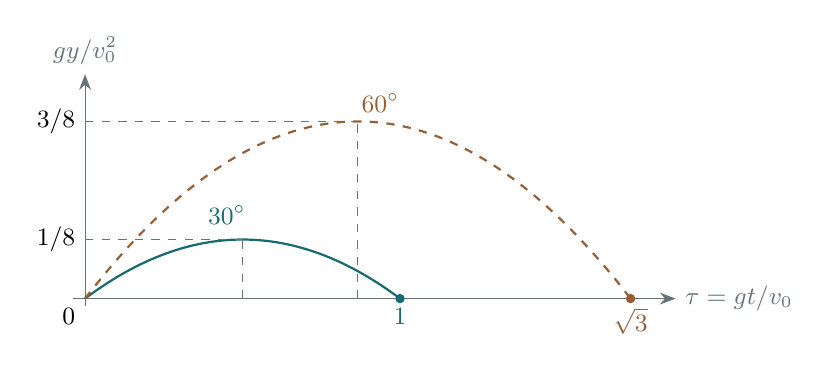
\begin{tikzpicture}
\draw[axis] (-.15,0)--(7.5,0) node[right] {$\tau=gt/v_0$};
\draw[axis] (0,-.1)--(0,2.85) node[above] {$gy/v_0^2$};
\draw[traj,domain=0:1,samples=70] plot({4*\x},{3*(\x-\x^2)});
\draw[thick,dashed,warm,domain=0:1.7320508,samples=80] plot({4*\x},{3*(sqrt(3)*\x-\x^2)});
\draw[guide] (2,0)--(2,.75);
\draw[guide] ({2*sqrt(3)},0)--({2*sqrt(3)},2.25);
\draw[guide] (0,.75)--(2,.75);\node[left] at (0,.75) {$1/8$};
\draw[guide] (0,2.25)--({2*sqrt(3)},2.25);\node[left] at (0,2.25) {$3/8$};
\fill[accent] (4,0) circle(1.7pt) node[below] {$1$};
\fill[warm] ({4*sqrt(3)},0) circle(1.7pt) node[below] {$\sqrt3$};
\node[above,accent] at (1.8,.82) {$30^\circ$};
\node[above,warm] at (3.75,2.24) {$60^\circ$};
\node[below left] at (0,0) {$0$};
\end{tikzpicture}
\figcaption{变图1.5V4\quad 两条高度曲线的右端分别标出两次飞行的结束时刻。}
\end{minipage}\end{center}
\item 已知较低发射角为 $\alpha_1<45^\circ$，求高、低轨迹的时间比和最高点高度比。由 $\alpha_2=\pi/2-\alpha_1$，
\[
\frac{T_2}{T_1}=\frac{\cos\alpha_1}{\sin\alpha_1}=\cot\alpha_1,\qquad
\frac{H_2}{H_1}=\left(\frac{T_2}{T_1}\right)^2=\cot^2\alpha_1.
\]
在 $30^\circ$ 处，上式给出时间比 $\sqrt3$ 和高度比3。变图1.5V5中，两曲线随发射角增大而下降，在 $45^\circ$ 处都趋于1。图中高度比变化更快，因为最高点高度正比于竖直初速度的平方。
\begin{center}\begin{minipage}{.98\linewidth}\centering
\begin{tikzpicture}[scale=.88,transform shape]
\draw[axis] (0,0.0000000)--(7.25,0.0000000) node[right] {$\alpha_1/(1^\circ)$};
\draw[axis] (0.0000000,0)--(0.0000000,2.8);
\node[above left] at (0.0000000,2.8) {$\text{比值}$};
\node[below,font=\scriptsize] at (0.0000000,-0.0800000) {$15$};
\node[below,font=\scriptsize] at (1.7500000,-0.0800000) {$22.5$};
\node[below,font=\scriptsize] at (3.5000000,-0.0800000) {$30$};
\node[below,font=\scriptsize] at (5.2500000,-0.0800000) {$37.5$};
\node[below,font=\scriptsize] at (7.0000000,-0.0800000) {$45$};
\node[left,font=\scriptsize] at (-0.0800000,0.0000000) {$0$};
\node[left,font=\scriptsize] at (-0.0800000,0.8333333) {$4.83$};
\node[left,font=\scriptsize] at (-0.0800000,1.6666667) {$9.67$};
\node[left,font=\scriptsize] at (-0.0800000,2.5000000) {$14.5$};
\draw[thick,color=accent] plot coordinates {(0.0000000,0.6434570) (0.0583333,0.6324065) (0.1166667,0.6217041) (0.1750000,0.6113332) (0.2333333,0.6012784) (0.2916667,0.5915249) (0.3500000,0.5820592) (0.4083333,0.5728683) (0.4666667,0.5639401) (0.5250000,0.5552632) (0.5833333,0.5468267) (0.6416667,0.5386205) (0.7000000,0.5306351) (0.7583333,0.5228613) (0.8166667,0.5152905) (0.8750000,0.5079147) (0.9333333,0.5007260) (0.9916667,0.4937173) (1.0500000,0.4868815) (1.1083333,0.4802122) (1.1666667,0.4737030) (1.2250000,0.4673480) (1.2833333,0.4611416) (1.3416667,0.4550784) (1.4000000,0.4491533) (1.4583333,0.4433613) (1.5166667,0.4376979) (1.5750000,0.4321586) (1.6333333,0.4267391) (1.6916667,0.4214354) (1.7500000,0.4162437) (1.8083333,0.4111602) (1.8666667,0.4061814) (1.9250000,0.4013040) (1.9833333,0.3965246) (2.0416667,0.3918402) (2.1000000,0.3872477) (2.1583333,0.3827444) (2.2166667,0.3783275) (2.2750000,0.3739944) (2.3333333,0.3697426) (2.3916667,0.3655696) (2.4500000,0.3614730) (2.5083333,0.3574508) (2.5666667,0.3535007) (2.6250000,0.3496206) (2.6833333,0.3458086) (2.7416667,0.3420627) (2.8000000,0.3383811) (2.8583333,0.3347621) (2.9166667,0.3312038) (2.9750000,0.3277047) (3.0333333,0.3242632) (3.0916667,0.3208777) (3.1500000,0.3175467) (3.2083333,0.3142688) (3.2666667,0.3110427) (3.3250000,0.3078670) (3.3833333,0.3047403) (3.4416667,0.3016616) (3.5000000,0.2986294) (3.5583333,0.2956428) (3.6166667,0.2927005) (3.6750000,0.2898015) (3.7333333,0.2869447) (3.7916667,0.2841291) (3.8500000,0.2813537) (3.9083333,0.2786176) (3.9666667,0.2759197) (4.0250000,0.2732593) (4.0833333,0.2706354) (4.1416667,0.2680473) (4.2000000,0.2654940) (4.2583333,0.2629747) (4.3166667,0.2604888) (4.3750000,0.2580355) (4.4333333,0.2556140) (4.4916667,0.2532236) (4.5500000,0.2508636) (4.6083333,0.2485335) (4.6666667,0.2462324) (4.7250000,0.2439599) (4.7833333,0.2417152) (4.8416667,0.2394979) (4.9000000,0.2373072) (4.9583333,0.2351427) (5.0166667,0.2330039) (5.0750000,0.2308901) (5.1333333,0.2288008) (5.1916667,0.2267356) (5.2500000,0.2246940) (5.3083333,0.2226755) (5.3666667,0.2206796) (5.4250000,0.2187059) (5.4833333,0.2167538) (5.5416667,0.2148231) (5.6000000,0.2129133) (5.6583333,0.2110239) (5.7166667,0.2091547) (5.7750000,0.2073051) (5.8333333,0.2054748) (5.8916667,0.2036634) (5.9500000,0.2018706) (6.0083333,0.2000961) (6.0666667,0.1983394) (6.1250000,0.1966003) (6.1833333,0.1948783) (6.2416667,0.1931733) (6.3000000,0.1914849) (6.3583333,0.1898128) (6.4166667,0.1881566) (6.4750000,0.1865162) (6.5333333,0.1848912) (6.5916667,0.1832813) (6.6500000,0.1816862) (6.7083333,0.1801058) (6.7666667,0.1785397) (6.8250000,0.1769877) (6.8833333,0.1754496) (6.9416667,0.1739250) (7.0000000,0.1724138)};
\draw[thick,color=accent] (7.65,2.4)--(8.1,2.4);\node[right,font=\scriptsize] at (8.15,2.4) {$T_2/T_1$};
\draw[thick,dashed,color=warm] plot coordinates {(0.0000000,2.4014144) (0.0583333,2.3196401) (0.1166667,2.2417924) (0.1750000,2.1676240) (0.2333333,2.0969068) (0.2916667,2.0294301) (0.3500000,1.9649990) (0.4083333,1.9034330) (0.4666667,1.8445650) (0.5250000,1.7882396) (0.5833333,1.7343127) (0.6416667,1.6826501) (0.7000000,1.6331269) (0.7583333,1.5856267) (0.8166667,1.5400410) (0.8750000,1.4962683) (0.9333333,1.4542139) (0.9916667,1.4137892) (1.0500000,1.3749110) (1.1083333,1.3375017) (1.1666667,1.3014883) (1.2250000,1.2668023) (1.2833333,1.2333793) (1.3416667,1.2011590) (1.4000000,1.1700843) (1.4583333,1.1401018) (1.5166667,1.1111609) (1.5750000,1.0832141) (1.6333333,1.0562164) (1.6916667,1.0301254) (1.7500000,1.0049012) (1.8083333,0.9805059) (1.8666667,0.9569035) (1.9250000,0.9340603) (1.9833333,0.9119441) (2.0416667,0.8905245) (2.1000000,0.8697726) (2.1583333,0.8496611) (2.2166667,0.8301640) (2.2750000,0.8112566) (2.3333333,0.7929155) (2.3916667,0.7751184) (2.4500000,0.7578440) (2.5083333,0.7410722) (2.5666667,0.7247838) (2.6250000,0.7089604) (2.6833333,0.6935847) (2.7416667,0.6786400) (2.8000000,0.6641103) (2.8583333,0.6499807) (2.9166667,0.6362366) (2.9750000,0.6228642) (3.0333333,0.6098504) (3.0916667,0.5971824) (3.1500000,0.5848483) (3.2083333,0.5728365) (3.2666667,0.5611359) (3.3250000,0.5497360) (3.3833333,0.5386267) (3.4416667,0.5277983) (3.5000000,0.5172414) (3.5583333,0.5069471) (3.6166667,0.4969069) (3.6750000,0.4871126) (3.7333333,0.4775562) (3.7916667,0.4682303) (3.8500000,0.4591276) (3.9083333,0.4502410) (3.9666667,0.4415639) (4.0250000,0.4330898) (4.0833333,0.4248126) (4.1416667,0.4167261) (4.2000000,0.4088248) (4.2583333,0.4011031) (4.3166667,0.3935557) (4.3750000,0.3861774) (4.4333333,0.3789633) (4.4916667,0.3719086) (4.5500000,0.3650088) (4.6083333,0.3582595) (4.6666667,0.3516563) (4.7250000,0.3451952) (4.7833333,0.3388722) (4.8416667,0.3326835) (4.9000000,0.3266254) (4.9583333,0.3206942) (5.0166667,0.3148867) (5.0750000,0.3091993) (5.1333333,0.3036290) (5.1916667,0.2981725) (5.2500000,0.2928270) (5.3083333,0.2875894) (5.3666667,0.2824570) (5.4250000,0.2774271) (5.4833333,0.2724969) (5.5416667,0.2676641) (5.6000000,0.2629260) (5.6583333,0.2582804) (5.7166667,0.2537249) (5.7750000,0.2492572) (5.8333333,0.2448753) (5.8916667,0.2405769) (5.9500000,0.2363601) (6.0083333,0.2322229) (6.0666667,0.2281634) (6.1250000,0.2241796) (6.1833333,0.2202699) (6.2416667,0.2164324) (6.3000000,0.2126655) (6.3583333,0.2089676) (6.4166667,0.2053369) (6.4750000,0.2017721) (6.5333333,0.1982715) (6.5916667,0.1948337) (6.6500000,0.1914573) (6.7083333,0.1881410) (6.7666667,0.1848833) (6.8250000,0.1816830) (6.8833333,0.1785388) (6.9416667,0.1754494) (7.0000000,0.1724138)};
\draw[thick,dashed,color=warm] (7.65,1.9)--(8.1,1.9);\node[right,font=\scriptsize] at (8.15,1.9) {$H_2/H_1$};
\end{tikzpicture}
\figcaption{变图1.5V5\quad 较高轨迹与较低轨迹的时间比及顶点高度比。}
\end{minipage}\end{center}
\end{enumerate}

\clearpage

\pdfbookmark[2]{第 6 题 水枪越墙的最小初速}{q6}

\section*{第 6 题\quad 水枪越墙的最小初速}

\tagline{M-01-06}

地面上的水枪枪口视为质点，与竖直墙的水平距离为 $d=3.0\,\mathrm m$，墙高为 $h=4.0\,\mathrm m$。水流以速率 $v_0$、仰角 $\alpha$ 喷出，忽略空气阻力和水流宽度，取 $g=10\,\mathrm{m/s^2}$。

求使水流恰好通过墙顶的最小初速及相应仰角。

\begin{center}
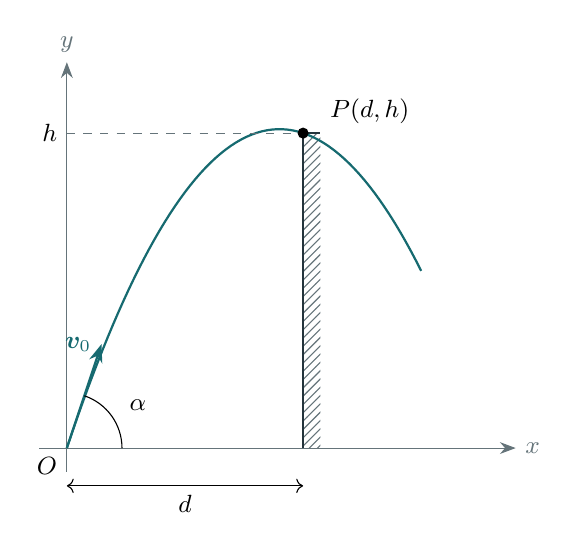
\begin{tikzpicture}[scale=1.0]
\draw[axis] (-.35,0)--(5.7,0) node[right] {$x$};\draw[axis] (0,-.3)--(0,4.9) node[above] {$y$};
\fill[pattern=north east lines,pattern color=muted] (3,0) rectangle (3.22,4);
\draw[object] (3,0)--(3,4)--(3.22,4);
\draw[traj,domain=0:4.5,samples=70] plot(\x,{3*\x-5*\x*\x/9});
\draw[motion] (0,0)--(.44,1.32) node[left] {$\vect v_0$};
\draw (.7,0) arc(0:71.565:.7);\node at (.9,.55) {$\alpha$};
\draw[guide] (0,4)--(3,4);\node[left] at (0,4) {$h$};
\draw[thin,<->] (0,-.48)--(3,-.48) node[midway,below] {$d$};
\fill (3,4) circle (2pt);\node[above right] at (3.22,4) {$P(d,h)$};\node[below left] at (0,0) {$O$};
\end{tikzpicture}
\figcaption{图 1.6\quad 枪口、墙顶与一条通过墙顶的轨迹。}
\end{center}

\Needspace{5\baselineskip}

\pdfbookmark[3]{题型定位}{q6-h0}

\subsection*{题型定位}

给定枪口和墙顶的位置，求刚好通过墙顶所需的最小发射速率。将轨迹经过 $(d,h)$ 的条件写成 $v_0^2(\alpha)$，然后在允许角度内找最小值。

\Needspace{5\baselineskip}

\pdfbookmark[3]{知识点}{q6-h1}

\subsection*{知识点}

斜抛轨迹由水平匀速和竖直匀变速消去时间得到。用 $p=\tan\alpha$ 求导可找极小值，也可借视线角 $\theta=\arctan(h/d)$ 和积化和差使分母最大。固定速率下对发射角求最高可达高度，得到抛物线族的包络。


\Needspace{5\baselineskip}

\pdfbookmark[3]{物理图像}{q6-h2}

\subsection*{物理图像}

解图1.6A中视线连接枪口与墙顶，初速度方向比视线更陡。随着初速降低，轨迹族包络在墙处降低。最低可行速率时包络刚过墙顶，解图1.6B所示的临界轨迹在墙前达到最高点，然后下降过墙。

\Needspace{5\baselineskip}

\pdfbookmark[3]{解题入口}{q6-h3}

\subsection*{解题入口}

将 $(d,h)$ 代入轨迹并解出 $v_0^2$。取 $p=\tan\alpha>h/d$，用商的求导法则得到二次分子 $dp^2-2hp-d$。取允许区间的根，再看两端的变化。代入最优速率和角度后，从 $t_d=d/v_{0x}$ 算出墙处竖直速度，用其符号说明图中上下行方向。

\Needspace{5\baselineskip}

\pdfbookmark[3]{标准解法}{q6-h4}

\subsection*{标准解法}

以枪口为原点，水平向墙为 $x$ 正向，竖直向上为 $y$ 正向。墙顶坐标为 $(d,h)$，解图 1.6A 中从枪口指向墙顶的直线与水平夹角记为 $\theta$，故 $\tan\theta=h/d$。
\begin{center}\begin{minipage}{\linewidth}\centering\begin{tikzpicture}

\draw[axis] (-.2,0)--(4.1,0) node[right] {$x$};\draw[axis] (0,-.2)--(0,4.6) node[above] {$y$};
\draw[object] (3,0)--(3,4);\fill (3,4) circle(2pt);\node[above right] at (3,4) {$P(d,h)$};
\draw[guide] (0,0)--(3,4) node[midway,above left,sloped] {$\sqrt{d^2+h^2}$};
\draw[motion] (0,0)--(.65,1.95) node[left] {$v_0$};
\draw (.68,0) arc(0:71.565:.68);\node at (.88,.7) {$\alpha$};
\draw (1.35,0) arc(0:53.13:1.35);\node at (1.55,.45) {$\theta$};
\draw[thin,<->] (0,-.55)--(3,-.55) node[midway,below] {$d$};
\draw[thin,<->] (3.45,0)--(3.45,4) node[midway,right] {$h$};
\node[align=left] at (6.45,2.8) {$\theta=\arctan(h/d)$\\$\alpha$：枪口仰角\\$\alpha>\theta$};

\end{tikzpicture}
\figcaption{解图 1.6A\quad $\theta$ 是墙顶的视线角，$\alpha$ 是发射角，$\alpha$沿枪口初速箭头量取。}
\end{minipage}\end{center}
\subsubsection*{通过墙顶的条件}
水流质点的轨迹为
\[
y=x\tan\alpha-\frac{gx^2}{2v_0^2\cos^2\alpha}.
\]
令 $x=d,y=h$，得
\[
v_0^2=\frac{gd^2}{2\cos^2\alpha(d\tan\alpha-h)}.
\]
式中 $v_0^2>0$ 给出 $\tan\alpha>h/d$。解图1.6A上，枪口切线在墙处的高度是 $d\tan\alpha$，抛物线比该高度低 $gd^2/(2v_0^2\cos^2\alpha)$。重力使轨迹低于枪口切线，所以切线在墙处的高度 $d\tan\alpha$ 高于 $h$，即 $\alpha>\theta$。
\subsubsection*{对发射角求最小初速}
记 $p=\tan\alpha>h/d$，则
\[
v_0^2(p)=\frac{gd^2}{2}\frac{1+p^2}{dp-h}.
\]
对 $p$ 求导，
\[
\frac{\dd v_0^2}{\dd p}
=\frac{gd^2}{2}\frac{2p(dp-h)-d(1+p^2)}{(dp-h)^2}
=\frac{gd^2}{2}\frac{dp^2-2hp-d}{(dp-h)^2}.
\]
驻点满足 $dp^2-2hp-d=0$。令 $s=\sqrt{d^2+h^2}$，两根为 $(h\pm s)/d$，只有正根符合发射角区间：
\[
p_* =\frac{h+s}{d}.
\]
$p\to h/d^+$ 或 $p\to\infty$ 时所需 $v_0^2$ 都趋于无穷；在允许区间仅有这个驻点，且导数由负变正，因此它给出全局最小值。代入后
\[
\boxed{v_{0,\min}^2=g(s+h)},\qquad
\boxed{\alpha_* =\arctan\frac{s+h}{d}
=\frac\pi4+\frac12\arctan\frac hd}.
\]
也可直接用视线角求极值。令 $\theta=\arctan(h/d)$，则 $d=s\cos\theta$、$h=s\sin\theta$。初速式的分母逐步变为
\[
\begin{aligned}
2\cos\alpha(d\sin\alpha-h\cos\alpha)
&=2s\cos\alpha\sin(\alpha-\theta)\\
&=s[\sin(2\alpha-\theta)-\sin\theta]\\
&=s\sin(2\alpha-\theta)-h.
\end{aligned}
\]
第二行来自积化和差，其中 $s\sin\theta=h$。整个分母随发射角变化，最大值为 $s-h$，因此
\[
v_0^2=\frac{gd^2}{s\sin(2\alpha-\theta)-h},
\]
分母在 $2\alpha-\theta=\pi/2$ 时最大，得到同一最优角。
\Needspace{0.46\textheight}
\subsubsection*{数值与墙顶处的运动状态}
本题 $s=5.0\,\mathrm m$，所以
\[
\boxed{v_{0,\min}=\sqrt{90}\approx9.49\,\mathrm{m/s},
\quad\alpha_* =\arctan3\approx71.57^\circ}.
\]
对应水平、竖直初速度分别为 $3.0$ 和 $9.0\,\mathrm{m/s}$。到墙时间 $t_d=d/v_{0x}=1.0\,\mathrm s$，此时
\[
y(t_d)=9.0\times1.0-5.0\times1.0^2=4.0\,\mathrm m,
\qquad v_y(t_d)=9.0-10\times1.0=-1.0\,\mathrm{m/s}.
\]
\begin{center}\begin{minipage}{\linewidth}\centering\begin{tikzpicture}

\draw[axis] (-.2,0)--(3.8,0) node[right] {$x/\mathrm m$};\draw[axis] (0,-.2)--(0,3.3) node[above] {$y/\mathrm m$};
\draw[traj,domain=2.2:3.3,samples=70] plot({3*(\x-2.2)},{9*(3*\x-5*\x*\x/9-3.8)});
\draw[object] (2.4,0)--(2.4,1.8);
\fill (1.5,2.25) circle(2pt);\node[above] at (1.5,2.25) {最高点 $Q$};
\fill (2.4,1.8) circle(2pt);\node[right] at (2.4,1.8) {墙顶 $P$};
\draw[guide] (1.5,0)--(1.5,2.25)--(0,2.25);\draw[guide] (0,1.8)--(2.4,1.8);
\node[below] at (1.5,0) {$2.7$};\node[below] at (2.4,0) {$3.0$};\node[left] at (0,2.25) {$4.05$};\node[left] at (0,1.8) {$4.00$};
\node[align=left] at (6.4,1.9) {最优轨迹到达墙顶时\\已经略向下运动。};

\end{tikzpicture}
\figcaption{解图 1.6B\quad 最小初速对应轨迹的局部放大图；横、纵方向使用不同显示比例。}
\end{minipage}\end{center}
因此水流经过墙顶时已经下降。最高点在 $t=0.90\,\mathrm s$，位置为 $(2.70,4.05)\,\mathrm m$，与解图 1.6B 的先后位置一致。一般最优轨迹在墙顶的斜率为 $-d/(s+h)<0$；墙顶的切线向右下方。解图1.6B中，从最高点到墙顶的水平距离是 $0.30\,\mathrm m$，高度下降 $0.05\,\mathrm m$，正对应这段飞行的 $0.10\,\mathrm s$。

\Needspace{5\baselineskip}

\pdfbookmark[3]{关键洞察}{q6-h5}

\subsection*{关键洞察}

临界的含义是改变发射角时，墙处高度达到该初速允许的最大值。沿轨迹的速度方向由对 $x$ 求导得到。本题在墙顶对角度的变化率为零，对 $x$ 的斜率为负，因而图1.6B在墙前已经过顶点。

\Needspace{5\baselineskip}

\pdfbookmark[3]{易错点}{q6-h6}

\subsection*{易错点}

\begin{itemize}
\item 角度从水平轴量起，过墙顶条件为 $\tan\alpha>h/d$。代入 $p$ 后按此区间选根。
\item 积化和差时保留 $2\cos\alpha\sin(\alpha-\theta)=\sin(2\alpha-\theta)-\sin\theta$ 中的后项。
\item $h>0$ 时 $\alpha_*=45^\circ+\theta/2>45^\circ$，$h=0$ 时回到 $45^\circ$ 和 $v_{0,\min}^2=gd$。
\item 图1.6B中墙顶坐标是 $(3.0,4.0)\,\mathrm m$，最高点是 $(2.70,4.05)\,\mathrm m$。前者的竖直速度为 $-1.0\,\mathrm{m/s}$。
\end{itemize}

\Needspace{5\baselineskip}

\pdfbookmark[3]{课堂讲解建议}{q6-h7}

\subsection*{课堂讲解建议}

先画墙顶视线，问“为何发射角比 $\theta$ 大”，答为重力使轨迹低于枪口处切线。求出 $\alpha_*$ 后，再问“在墙处水流向上还是向下”。由 $v_{0x}=3\,\mathrm{m/s}$、$v_{0y}=9\,\mathrm{m/s}$，算出到墙用时一秒，墙处 $v_y=-1\,\mathrm{m/s}$。随后把解图1.6B的最高点与墙顶连起来，标出 $0.30\,\mathrm m$ 的水平距离。若用变图1.6V3解释包络，指出对发射角取极值选出通过墙顶的轨迹，沿这条轨迹的最高点由 $v_y=0$ 定位。

\Needspace{5\baselineskip}

\pdfbookmark[3]{变式训练}{q6-h8}

\subsection*{变式训练}

\begin{enumerate}
\item 固定墙高 $h>0$，增大距离 $d$，求最优角和最小速率的变化。由 $\alpha_*=\pi/4+\tfrac12\arctan(h/d)$，
\[
\frac{\dd\alpha_*}{\dd d}=-\frac{h}{2(d^2+h^2)}<0,\qquad
\frac{\dd v_{\min}^2}{\dd d}=\frac{gd}{\sqrt{d^2+h^2}}>0.
\]
变图1.6V1的横坐标是 $d/h$。从图上向右读，视线角逐渐减小，最优角由接近 $90^\circ$ 逐渐趋于 $45^\circ$。例如 $d=h$ 时，最优角为 $67.5^\circ$，$v_{\min}^2=g(1+\sqrt2)h$。
\begin{center}\begin{minipage}{.98\linewidth}\centering
\begin{tikzpicture}[scale=.88,transform shape]
\draw[axis] (0,0.0000000)--(7.25,0.0000000) node[right] {$d/h$};
\draw[axis] (0.0000000,0)--(0.0000000,2.8);
\node[above left] at (0.0000000,2.8) {$\alpha_*/(1^\circ)$};
\node[below,font=\scriptsize] at (0.0000000,-0.0800000) {$0.15$};
\node[below,font=\scriptsize] at (1.7500000,-0.0800000) {$1.36$};
\node[below,font=\scriptsize] at (3.5000000,-0.0800000) {$2.57$};
\node[below,font=\scriptsize] at (5.2500000,-0.0800000) {$3.79$};
\node[below,font=\scriptsize] at (7.0000000,-0.0800000) {$5$};
\node[left,font=\scriptsize] at (-0.0800000,0.0000000) {$45$};
\node[left,font=\scriptsize] at (-0.0800000,0.8333333) {$60$};
\node[left,font=\scriptsize] at (-0.0800000,1.6666667) {$75$};
\node[left,font=\scriptsize] at (-0.0800000,2.5000000) {$90$};
\draw[thick,color=accent] plot coordinates {(0.0000000,2.2630343) (0.0583333,2.2005276) (0.1166667,2.1389416) (0.1750000,2.0784359) (0.2333333,2.0191523) (0.2916667,1.9612134) (0.3500000,1.9047220) (0.4083333,1.8497614) (0.4666667,1.7963957) (0.5250000,1.7446713) (0.5833333,1.6946178) (0.6416667,1.6462497) (0.7000000,1.5995681) (0.7583333,1.5545626) (0.8166667,1.5112125) (0.8750000,1.4694891) (0.9333333,1.4293566) (0.9916667,1.3907739) (1.0500000,1.3536958) (1.1083333,1.3180739) (1.1666667,1.2838576) (1.2250000,1.2509953) (1.2833333,1.2194346) (1.3416667,1.1891229) (1.4000000,1.1600083) (1.4583333,1.1320397) (1.5166667,1.1051670) (1.5750000,1.0793414) (1.6333333,1.0545158) (1.6916667,1.0306446) (1.7500000,1.0076839) (1.8083333,0.9855916) (1.8666667,0.9643275) (1.9250000,0.9438530) (1.9833333,0.9241314) (2.0416667,0.9051275) (2.1000000,0.8868081) (2.1583333,0.8691414) (2.2166667,0.8520973) (2.2750000,0.8356472) (2.3333333,0.8197638) (2.3916667,0.8044215) (2.4500000,0.7895956) (2.5083333,0.7752631) (2.5666667,0.7614018) (2.6250000,0.7479911) (2.6833333,0.7350109) (2.7416667,0.7224426) (2.8000000,0.7102685) (2.8583333,0.6984715) (2.9166667,0.6870356) (2.9750000,0.6759458) (3.0333333,0.6651874) (3.0916667,0.6547469) (3.1500000,0.6446112) (3.2083333,0.6347679) (3.2666667,0.6252052) (3.3250000,0.6159121) (3.3833333,0.6068778) (3.4416667,0.5980924) (3.5000000,0.5895460) (3.5583333,0.5812297) (3.6166667,0.5731346) (3.6750000,0.5652524) (3.7333333,0.5575753) (3.7916667,0.5500956) (3.8500000,0.5428062) (3.9083333,0.5357002) (3.9666667,0.5287711) (4.0250000,0.5220125) (4.0833333,0.5154185) (4.1416667,0.5089833) (4.2000000,0.5027016) (4.2583333,0.4965680) (4.3166667,0.4905775) (4.3750000,0.4847254) (4.4333333,0.4790071) (4.4916667,0.4734182) (4.5500000,0.4679544) (4.6083333,0.4626118) (4.6666667,0.4573865) (4.7250000,0.4522747) (4.7833333,0.4472730) (4.8416667,0.4423778) (4.9000000,0.4375859) (4.9583333,0.4328942) (5.0166667,0.4282996) (5.0750000,0.4237992) (5.1333333,0.4193902) (5.1916667,0.4150700) (5.2500000,0.4108359) (5.3083333,0.4066854) (5.3666667,0.4026162) (5.4250000,0.3986259) (5.4833333,0.3947123) (5.5416667,0.3908733) (5.6000000,0.3871067) (5.6583333,0.3834107) (5.7166667,0.3797832) (5.7750000,0.3762225) (5.8333333,0.3727267) (5.8916667,0.3692941) (5.9500000,0.3659230) (6.0083333,0.3626119) (6.0666667,0.3593592) (6.1250000,0.3561633) (6.1833333,0.3530228) (6.2416667,0.3499364) (6.3000000,0.3469025) (6.3583333,0.3439201) (6.4166667,0.3409877) (6.4750000,0.3381041) (6.5333333,0.3352682) (6.5916667,0.3324787) (6.6500000,0.3297347) (6.7083333,0.3270349) (6.7666667,0.3243784) (6.8250000,0.3217641) (6.8833333,0.3191910) (6.9416667,0.3166582) (7.0000000,0.3141648)};
\end{tikzpicture}
\figcaption{变图1.6V1\quad 固定墙高，最优角随墙距增大而减小。}
\end{minipage}\end{center}
\item 枪口下方留有飞行空间，目标相对枪口的坐标为$(d,h)$，其中$h<0,d>0$。求最优发射角及速率。记 $s=\sqrt{d^2+h^2}>|h|$。优化方程的允许根仍为 $p_*=(s+h)/d>0$，因而
\[
0<\alpha_*=\frac\pi4+\frac12\arctan(h/d)<\frac\pi4,
\qquad v_{\min}^2=g(s+h)>0.
\]
变图1.6V2取 $d=4\,\mathrm m,h=-3\,\mathrm m$，此时 $p_*=1/2$、$v_{\min}^2=2g\,\mathrm m$，归一化轨迹为 $y/d=(x/d)/2-5(x/d)^2/4$。由图上的顶点可见，该发射角使水流先升后降，最后到达较低目标。
\begin{center}\begin{minipage}{.98\linewidth}\centering
\begin{tikzpicture}[scale=.88,transform shape]
\draw[axis] (0,2.2471910)--(7.25,2.2471910) node[right] {$x/d$};
\draw[axis] (0.0000000,0)--(0.0000000,2.8);
\node[above left] at (0.0000000,2.8) {$y/d$};
\node[below,font=\scriptsize] at (0.0000000,2.1671910) {$0$};
\node[below,font=\scriptsize] at (1.7500000,2.1671910) {$0.25$};
\node[below,font=\scriptsize] at (3.5000000,2.1671910) {$0.5$};
\node[below,font=\scriptsize] at (5.2500000,2.1671910) {$0.75$};
\node[below,font=\scriptsize] at (7.0000000,2.1671910) {$1$};
\node[left,font=\scriptsize] at (-0.0800000,0.0000000) {$-0.8$};
\node[left,font=\scriptsize] at (-0.0800000,0.8333333) {$-0.503$};
\node[left,font=\scriptsize] at (-0.0800000,1.6666667) {$-0.207$};
\node[left,font=\scriptsize] at (-0.0800000,2.5000000) {$0.09$};
\draw[thick,color=accent] plot coordinates {(0.0000000,2.2471910) (0.0583333,2.2586513) (0.1166667,2.2696239) (0.1750000,2.2801088) (0.2333333,2.2901061) (0.2916667,2.2996157) (0.3500000,2.3086376) (0.4083333,2.3171719) (0.4666667,2.3252185) (0.5250000,2.3327774) (0.5833333,2.3398486) (0.6416667,2.3464322) (0.7000000,2.3525281) (0.7583333,2.3581363) (0.8166667,2.3632569) (0.8750000,2.3678897) (0.9333333,2.3720350) (0.9916667,2.3756925) (1.0500000,2.3788624) (1.1083333,2.3815446) (1.1666667,2.3837391) (1.2250000,2.3854459) (1.2833333,2.3866651) (1.3416667,2.3873966) (1.4000000,2.3876404) (1.4583333,2.3873966) (1.5166667,2.3866651) (1.5750000,2.3854459) (1.6333333,2.3837391) (1.6916667,2.3815446) (1.7500000,2.3788624) (1.8083333,2.3756925) (1.8666667,2.3720350) (1.9250000,2.3678897) (1.9833333,2.3632569) (2.0416667,2.3581363) (2.1000000,2.3525281) (2.1583333,2.3464322) (2.2166667,2.3398486) (2.2750000,2.3327774) (2.3333333,2.3252185) (2.3916667,2.3171719) (2.4500000,2.3086376) (2.5083333,2.2996157) (2.5666667,2.2901061) (2.6250000,2.2801088) (2.6833333,2.2696239) (2.7416667,2.2586513) (2.8000000,2.2471910) (2.8583333,2.2352431) (2.9166667,2.2228074) (2.9750000,2.2098841) (3.0333333,2.1964732) (3.0916667,2.1825745) (3.1500000,2.1681882) (3.2083333,2.1533142) (3.2666667,2.1379526) (3.3250000,2.1221032) (3.3833333,2.1057662) (3.4416667,2.0889416) (3.5000000,2.0716292) (3.5583333,2.0538292) (3.6166667,2.0355415) (3.6750000,2.0167662) (3.7333333,1.9975031) (3.7916667,1.9777524) (3.8500000,1.9575140) (3.9083333,1.9367880) (3.9666667,1.9155743) (4.0250000,1.8938729) (4.0833333,1.8716838) (4.1416667,1.8490071) (4.2000000,1.8258427) (4.2583333,1.8021906) (4.3166667,1.7780509) (4.3750000,1.7534235) (4.4333333,1.7283084) (4.4916667,1.7027056) (4.5500000,1.6766152) (4.6083333,1.6500371) (4.6666667,1.6229713) (4.7250000,1.5954178) (4.7833333,1.5673767) (4.8416667,1.5388479) (4.9000000,1.5098315) (4.9583333,1.4803273) (5.0166667,1.4503355) (5.0750000,1.4198560) (5.1333333,1.3888889) (5.1916667,1.3574341) (5.2500000,1.3254916) (5.3083333,1.2930614) (5.3666667,1.2601436) (5.4250000,1.2267381) (5.4833333,1.1928449) (5.5416667,1.1584640) (5.6000000,1.1235955) (5.6583333,1.0882393) (5.7166667,1.0523954) (5.7750000,1.0160639) (5.8333333,0.9792447) (5.8916667,0.9419378) (5.9500000,0.9041433) (6.0083333,0.8658610) (6.0666667,0.8270911) (6.1250000,0.7878336) (6.1833333,0.7480883) (6.2416667,0.7078554) (6.3000000,0.6671348) (6.3583333,0.6259266) (6.4166667,0.5842306) (6.4750000,0.5420471) (6.5333333,0.4993758) (6.5916667,0.4562168) (6.6500000,0.4125702) (6.7083333,0.3684359) (6.7666667,0.3238140) (6.8250000,0.2787044) (6.8833333,0.2331071) (6.9416667,0.1870221) (7.0000000,0.1404494)};
\fill[accent] (7.0000000,0.1404494) circle(1.7pt) node[above right] {$P$};
\end{tikzpicture}
\figcaption{变图1.6V2\quad 较低目标位于 $(x/d,y/d)=(1,-0.75)$，最优轨迹仍先上升。}
\end{minipage}\end{center}
\item 用轨迹族包络求任意目标点 $(d,h)$ 的最小初速。置 $p=\tan\alpha$，固定 $v_0$ 与 $x>0$。对 $y=xp-gx^2(1+p^2)/(2v_0^2)$ 配方，得
\[
y=\frac{v_0^2}{2g}-\frac{gx^2}{2v_0^2}
-\frac{gx^2}{2v_0^2}\left(p-\frac{v_0^2}{gx}\right)^2.
\]
前两项为包络，平方项为零处相切。令 $x=d$ 处的包络高度恰为 $h$，得到 $v_0^4-2ghv_0^2-g^2d^2=0$，正根是 $v_{\min}^2=g(s+h)$。变图1.6V3以 $d=3\,\mathrm m,h=4\,\mathrm m$ 为例，$v_0^2/(gd)=3$，在 $x=d$ 相切的曲线为 $p=3$。
\begin{center}\begin{minipage}{.98\linewidth}\centering
\begin{tikzpicture}[scale=.88,transform shape]
\draw[axis] (0,0.0000000)--(7.25,0.0000000) node[right] {$x/d$};
\draw[axis] (0.0000000,0)--(0.0000000,2.8);
\node[above left] at (0.0000000,2.8) {$y/d$};
\node[below,font=\scriptsize] at (0.0000000,-0.0800000) {$0.15$};
\node[below,font=\scriptsize] at (1.7500000,-0.0800000) {$0.412$};
\node[below,font=\scriptsize] at (3.5000000,-0.0800000) {$0.675$};
\node[below,font=\scriptsize] at (5.2500000,-0.0800000) {$0.938$};
\node[below,font=\scriptsize] at (7.0000000,-0.0800000) {$1.2$};
\node[left,font=\scriptsize] at (-0.0800000,0.0000000) {$0$};
\node[left,font=\scriptsize] at (-0.0800000,0.8333333) {$0.517$};
\node[left,font=\scriptsize] at (-0.0800000,1.6666667) {$1.03$};
\node[left,font=\scriptsize] at (-0.0800000,2.5000000) {$1.55$};
\draw[thick,color=accent] plot coordinates {(0.0000000,0.4536290) (0.0583333,0.4782237) (0.1166667,0.5026126) (0.1750000,0.5267956) (0.2333333,0.5507728) (0.2916667,0.5745443) (0.3500000,0.5981099) (0.4083333,0.6214697) (0.4666667,0.6446237) (0.5250000,0.6675718) (0.5833333,0.6903142) (0.6416667,0.7128507) (0.7000000,0.7351815) (0.7583333,0.7573064) (0.8166667,0.7792255) (0.8750000,0.8009388) (0.9333333,0.8224462) (0.9916667,0.8437479) (1.0500000,0.8648438) (1.1083333,0.8857338) (1.1666667,0.9064180) (1.2250000,0.9268964) (1.2833333,0.9471690) (1.3416667,0.9672358) (1.4000000,0.9870968) (1.4583333,1.0067519) (1.5166667,1.0262013) (1.5750000,1.0454448) (1.6333333,1.0644825) (1.6916667,1.0833144) (1.7500000,1.1019405) (1.8083333,1.1203608) (1.8666667,1.1385753) (1.9250000,1.1565839) (1.9833333,1.1743868) (2.0416667,1.1919838) (2.1000000,1.2093750) (2.1583333,1.2265604) (2.2166667,1.2435400) (2.2750000,1.2603138) (2.3333333,1.2768817) (2.3916667,1.2932439) (2.4500000,1.3094002) (2.5083333,1.3253507) (2.5666667,1.3410954) (2.6250000,1.3566343) (2.6833333,1.3719674) (2.7416667,1.3870947) (2.8000000,1.4020161) (2.8583333,1.4167318) (2.9166667,1.4312416) (2.9750000,1.4455456) (3.0333333,1.4596438) (3.0916667,1.4735362) (3.1500000,1.4872228) (3.2083333,1.5007035) (3.2666667,1.5139785) (3.3250000,1.5270476) (3.3833333,1.5399110) (3.4416667,1.5525685) (3.5000000,1.5650202) (3.5583333,1.5772660) (3.6166667,1.5893061) (3.6750000,1.6011404) (3.7333333,1.6127688) (3.7916667,1.6241914) (3.8500000,1.6354083) (3.9083333,1.6464193) (3.9666667,1.6572245) (4.0250000,1.6678238) (4.0833333,1.6782174) (4.1416667,1.6884052) (4.2000000,1.6983871) (4.2583333,1.7081632) (4.3166667,1.7177335) (4.3750000,1.7270980) (4.4333333,1.7362567) (4.4916667,1.7452096) (4.5500000,1.7539567) (4.6083333,1.7624979) (4.6666667,1.7708333) (4.7250000,1.7789630) (4.7833333,1.7868868) (4.8416667,1.7946048) (4.9000000,1.8021169) (4.9583333,1.8094233) (5.0166667,1.8165239) (5.0750000,1.8234186) (5.1333333,1.8301075) (5.1916667,1.8365906) (5.2500000,1.8428679) (5.3083333,1.8489394) (5.3666667,1.8548051) (5.4250000,1.8604650) (5.4833333,1.8659190) (5.5416667,1.8711673) (5.6000000,1.8762097) (5.6583333,1.8810463) (5.7166667,1.8856771) (5.7750000,1.8901021) (5.8333333,1.8943212) (5.8916667,1.8983346) (5.9500000,1.9021421) (6.0083333,1.9057439) (6.0666667,1.9091398) (6.1250000,1.9123299) (6.1833333,1.9153142) (6.2416667,1.9180927) (6.3000000,1.9206653) (6.3583333,1.9230322) (6.4166667,1.9251932) (6.4750000,1.9271484) (6.5333333,1.9288978) (6.5916667,1.9304414) (6.6500000,1.9317792) (6.7083333,1.9329112) (6.7666667,1.9338374) (6.8250000,1.9345577) (6.8833333,1.9350722) (6.9416667,1.9353810) (7.0000000,1.9354839)};
\draw[thick,color=accent] (7.65,2.4)--(8.1,2.4);\node[right,font=\scriptsize] at (8.15,2.4) {$p=2$};
\draw[thick,dashed,color=warm] plot coordinates {(0.0000000,0.6653226) (0.0583333,0.7003990) (0.1166667,0.7350638) (0.1750000,0.7693170) (0.2333333,0.8031586) (0.2916667,0.8365885) (0.3500000,0.8696069) (0.4083333,0.9022135) (0.4666667,0.9344086) (0.5250000,0.9661920) (0.5833333,0.9975638) (0.6416667,1.0285240) (0.7000000,1.0590726) (0.7583333,1.0892095) (0.8166667,1.1189348) (0.8750000,1.1482485) (0.9333333,1.1771505) (0.9916667,1.2056410) (1.0500000,1.2337198) (1.1083333,1.2613869) (1.1666667,1.2886425) (1.2250000,1.3154864) (1.2833333,1.3419187) (1.3416667,1.3679393) (1.4000000,1.3935484) (1.4583333,1.4187458) (1.5166667,1.4435316) (1.5750000,1.4679057) (1.6333333,1.4918683) (1.6916667,1.5154192) (1.7500000,1.5385585) (1.8083333,1.5612861) (1.8666667,1.5836022) (1.9250000,1.6055066) (1.9833333,1.6269993) (2.0416667,1.6480805) (2.1000000,1.6687500) (2.1583333,1.6890079) (2.2166667,1.7088542) (2.2750000,1.7282888) (2.3333333,1.7473118) (2.3916667,1.7659232) (2.4500000,1.7841230) (2.5083333,1.8019111) (2.5666667,1.8192876) (2.6250000,1.8362525) (2.6833333,1.8528058) (2.7416667,1.8689474) (2.8000000,1.8846774) (2.8583333,1.8999958) (2.9166667,1.9149026) (2.9750000,1.9293977) (3.0333333,1.9434812) (3.0916667,1.9571531) (3.1500000,1.9704133) (3.2083333,1.9832619) (3.2666667,1.9956989) (3.3250000,2.0077243) (3.3833333,2.0193380) (3.4416667,2.0305402) (3.5000000,2.0413306) (3.5583333,2.0517095) (3.6166667,2.0616767) (3.6750000,2.0712324) (3.7333333,2.0803763) (3.7916667,2.0891087) (3.8500000,2.0974294) (3.9083333,2.1053385) (3.9666667,2.1128360) (4.0250000,2.1199219) (4.0833333,2.1265961) (4.1416667,2.1328587) (4.2000000,2.1387097) (4.2583333,2.1441490) (4.3166667,2.1491767) (4.3750000,2.1537928) (4.4333333,2.1579973) (4.4916667,2.1617902) (4.5500000,2.1651714) (4.6083333,2.1681410) (4.6666667,2.1706989) (4.7250000,2.1728453) (4.7833333,2.1745800) (4.8416667,2.1759031) (4.9000000,2.1768145) (4.9583333,2.1773143) (5.0166667,2.1774026) (5.0750000,2.1770791) (5.1333333,2.1763441) (5.1916667,2.1751974) (5.2500000,2.1736391) (5.3083333,2.1716692) (5.3666667,2.1692876) (5.4250000,2.1664945) (5.4833333,2.1632897) (5.5416667,2.1596732) (5.6000000,2.1556452) (5.6583333,2.1512055) (5.7166667,2.1463542) (5.7750000,2.1410912) (5.8333333,2.1354167) (5.8916667,2.1293305) (5.9500000,2.1228327) (6.0083333,2.1159232) (6.0666667,2.1086022) (6.1250000,2.1008695) (6.1833333,2.0927251) (6.2416667,2.0841692) (6.3000000,2.0752016) (6.3583333,2.0658224) (6.4166667,2.0560316) (6.4750000,2.0458291) (6.5333333,2.0352151) (6.5916667,2.0241893) (6.6500000,2.0127520) (6.7083333,2.0009031) (6.7666667,1.9886425) (6.8250000,1.9759703) (6.8833333,1.9628864) (6.9416667,1.9493910) (7.0000000,1.9354839)};
\draw[thick,dashed,color=warm] (7.65,1.9)--(8.1,1.9);\node[right,font=\scriptsize] at (8.15,1.9) {$p=3$};
\draw[thick,densely dotted,color=muted] plot coordinates {(0.0000000,0.8649194) (0.0583333,0.9090251) (0.1166667,0.9524311) (0.1750000,0.9951373) (0.2333333,1.0371438) (0.2916667,1.0784505) (0.3500000,1.1190575) (0.4083333,1.1589646) (0.4666667,1.1981720) (0.5250000,1.2366797) (0.5833333,1.2744876) (0.6416667,1.3115957) (0.7000000,1.3480040) (0.7583333,1.3837126) (0.8166667,1.4187214) (0.8750000,1.4530305) (0.9333333,1.4866398) (0.9916667,1.5195493) (1.0500000,1.5517591) (1.1083333,1.5832691) (1.1666667,1.6140793) (1.2250000,1.6441898) (1.2833333,1.6736005) (1.3416667,1.7023114) (1.4000000,1.7303226) (1.4583333,1.7576340) (1.5166667,1.7842456) (1.5750000,1.8101575) (1.6333333,1.8353696) (1.6916667,1.8598820) (1.7500000,1.8836946) (1.8083333,1.9068074) (1.8666667,1.9292204) (1.9250000,1.9509337) (1.9833333,1.9719472) (2.0416667,1.9922610) (2.1000000,2.0118750) (2.1583333,2.0307892) (2.2166667,2.0490037) (2.2750000,2.0665184) (2.3333333,2.0833333) (2.3916667,2.0994485) (2.4500000,2.1148639) (2.5083333,2.1295796) (2.5666667,2.1435954) (2.6250000,2.1569115) (2.6833333,2.1695279) (2.7416667,2.1814445) (2.8000000,2.1926613) (2.8583333,2.2031783) (2.9166667,2.2129956) (2.9750000,2.2221132) (3.0333333,2.2305309) (3.0916667,2.2382489) (3.1500000,2.2452671) (3.2083333,2.2515856) (3.2666667,2.2572043) (3.3250000,2.2621232) (3.3833333,2.2663424) (3.4416667,2.2698618) (3.5000000,2.2726815) (3.5583333,2.2748013) (3.6166667,2.2762214) (3.6750000,2.2769418) (3.7333333,2.2769624) (3.7916667,2.2762832) (3.8500000,2.2749042) (3.9083333,2.2728255) (3.9666667,2.2700470) (4.0250000,2.2665688) (4.0833333,2.2623908) (4.1416667,2.2575130) (4.2000000,2.2519355) (4.2583333,2.2456582) (4.3166667,2.2386811) (4.3750000,2.2310043) (4.4333333,2.2226277) (4.4916667,2.2135513) (4.5500000,2.2037752) (4.6083333,2.1932993) (4.6666667,2.1821237) (4.7250000,2.1702482) (4.7833333,2.1576731) (4.8416667,2.1443981) (4.9000000,2.1304234) (4.9583333,2.1157489) (5.0166667,2.1003747) (5.0750000,2.0843007) (5.1333333,2.0675269) (5.1916667,2.0500533) (5.2500000,2.0318800) (5.3083333,2.0130070) (5.3666667,1.9934341) (5.4250000,1.9731615) (5.4833333,1.9521892) (5.5416667,1.9305171) (5.6000000,1.9081452) (5.6583333,1.8850735) (5.7166667,1.8613021) (5.7750000,1.8368309) (5.8333333,1.8116599) (5.8916667,1.7857892) (5.9500000,1.7592187) (6.0083333,1.7319485) (6.0666667,1.7039785) (6.1250000,1.6753087) (6.1833333,1.6459392) (6.2416667,1.6158699) (6.3000000,1.5851008) (6.3583333,1.5536320) (6.4166667,1.5214634) (6.4750000,1.4885950) (6.5333333,1.4550269) (6.5916667,1.4207590) (6.6500000,1.3857913) (6.7083333,1.3501239) (6.7666667,1.3137567) (6.8250000,1.2766898) (6.8833333,1.2389231) (6.9416667,1.2004566) (7.0000000,1.1612903)};
\draw[thick,densely dotted,color=muted] (7.65,1.4)--(8.1,1.4);\node[right,font=\scriptsize] at (8.15,1.4) {$p=4$};
\draw[very thick,color=ink] plot coordinates {(0.0000000,2.4133065) (0.0583333,2.4125802) (0.1166667,2.4118128) (0.1750000,2.4110043) (0.2333333,2.4101546) (0.2916667,2.4092637) (0.3500000,2.4083317) (0.4083333,2.4073585) (0.4666667,2.4063441) (0.5250000,2.4052886) (0.5833333,2.4041919) (0.6416667,2.4030540) (0.7000000,2.4018750) (0.7583333,2.4006548) (0.8166667,2.3993935) (0.8750000,2.3980910) (0.9333333,2.3967473) (0.9916667,2.3953625) (1.0500000,2.3939365) (1.1083333,2.3924693) (1.1666667,2.3909610) (1.2250000,2.3894115) (1.2833333,2.3878209) (1.3416667,2.3861891) (1.4000000,2.3845161) (1.4583333,2.3828020) (1.5166667,2.3810467) (1.5750000,2.3792503) (1.6333333,2.3774126) (1.6916667,2.3755339) (1.7500000,2.3736139) (1.8083333,2.3716528) (1.8666667,2.3696505) (1.9250000,2.3676071) (1.9833333,2.3655225) (2.0416667,2.3633968) (2.1000000,2.3612298) (2.1583333,2.3590218) (2.2166667,2.3567725) (2.2750000,2.3544821) (2.3333333,2.3521505) (2.3916667,2.3497778) (2.4500000,2.3473639) (2.5083333,2.3449089) (2.5666667,2.3424126) (2.6250000,2.3398753) (2.6833333,2.3372967) (2.7416667,2.3346770) (2.8000000,2.3320161) (2.8583333,2.3293141) (2.9166667,2.3265709) (2.9750000,2.3237865) (3.0333333,2.3209610) (3.0916667,2.3180943) (3.1500000,2.3151865) (3.2083333,2.3122375) (3.2666667,2.3092473) (3.3250000,2.3062160) (3.3833333,2.3031435) (3.4416667,2.3000298) (3.5000000,2.2968750) (3.5583333,2.2936790) (3.6166667,2.2904419) (3.6750000,2.2871636) (3.7333333,2.2838441) (3.7916667,2.2804835) (3.8500000,2.2770817) (3.9083333,2.2736387) (3.9666667,2.2701546) (4.0250000,2.2666293) (4.0833333,2.2630628) (4.1416667,2.2594552) (4.2000000,2.2558065) (4.2583333,2.2521165) (4.3166667,2.2483854) (4.3750000,2.2446132) (4.4333333,2.2407997) (4.4916667,2.2369451) (4.5500000,2.2330494) (4.6083333,2.2291125) (4.6666667,2.2251344) (4.7250000,2.2211152) (4.7833333,2.2170548) (4.8416667,2.2129532) (4.9000000,2.2088105) (4.9583333,2.2046266) (5.0166667,2.2004015) (5.0750000,2.1961353) (5.1333333,2.1918280) (5.1916667,2.1874794) (5.2500000,2.1830897) (5.3083333,2.1786589) (5.3666667,2.1741868) (5.4250000,2.1696736) (5.4833333,2.1651193) (5.5416667,2.1605238) (5.6000000,2.1558871) (5.6583333,2.1512093) (5.7166667,2.1464903) (5.7750000,2.1417301) (5.8333333,2.1369288) (5.8916667,2.1320863) (5.9500000,2.1272026) (6.0083333,2.1222778) (6.0666667,2.1173118) (6.1250000,2.1123047) (6.1833333,2.1072564) (6.2416667,2.1021669) (6.3000000,2.0970363) (6.3583333,2.0918645) (6.4166667,2.0866515) (6.4750000,2.0813974) (6.5333333,2.0761022) (6.5916667,2.0707657) (6.6500000,2.0653881) (6.7083333,2.0599693) (6.7666667,2.0545094) (6.8250000,2.0490083) (6.8833333,2.0434661) (6.9416667,2.0378826) (7.0000000,2.0322581)};
\draw[very thick,color=ink] (7.65,0.8999999999999999)--(8.1,0.8999999999999999);\node[right,font=\scriptsize] at (8.15,0.8999999999999999) {$\text{包络}$};
\fill[ink] (5.6666667,2.1505352) circle(1.7pt) node[above right] {$P$};
\end{tikzpicture}
\figcaption{变图1.6V3\quad 包络与 $p=3$ 的轨迹在墙顶相切。}
\end{minipage}\end{center}
\item 水流还须落在墙后地面的 $x=D>d$，水流在墙处达到至少$h$，求最小初速。将落点 $D$ 代入轨迹，得到
\[
v_0^2=\frac{gD}{2}(p+1/p),\qquad y(x)=xp(1-x/D).
\]
墙处要求 $p\ge p_h=hD/[d(D-d)]$，同时 $p>0$。函数 $p+1/p$ 的导数为 $1-1/p^2$，在 $0<p<1$ 时为负，在 $p>1$ 时为正。若 $p_h\le1$，取 $p_*=1$ 即可越墙；若 $p_h>1$，最小的可行角由 $p_*=p_h$ 给出。要求恰好通过墙顶时取 $p=p_h$。变图1.6V4取 $D=6\,\mathrm m,d=3\,\mathrm m,h=4\,\mathrm m$，此时 $p_h=8/3$，$p=1$ 只能在墙处达到 $1.5\,\mathrm m$，故最优可行轨迹取 $p_*=8/3$，$v_0^2=91.25\,\mathrm{m^2/s^2}$（$g=10\,\mathrm{m/s^2}$）。
\begin{center}\begin{minipage}{.98\linewidth}\centering
\begin{tikzpicture}[scale=.88,transform shape]
\draw[axis] (0,0.0000000)--(7.25,0.0000000) node[right] {$x/D$};
\draw[axis] (0.0000000,0)--(0.0000000,2.8);
\node[above left] at (0.0000000,2.8) {$y/D$};
\node[below,font=\scriptsize] at (0.0000000,-0.0800000) {$0$};
\node[below,font=\scriptsize] at (1.7500000,-0.0800000) {$0.25$};
\node[below,font=\scriptsize] at (3.5000000,-0.0800000) {$0.5$};
\node[below,font=\scriptsize] at (5.2500000,-0.0800000) {$0.75$};
\node[below,font=\scriptsize] at (7.0000000,-0.0800000) {$1$};
\node[left,font=\scriptsize] at (-0.0800000,0.0000000) {$0$};
\node[left,font=\scriptsize] at (-0.0800000,0.8333333) {$0.233$};
\node[left,font=\scriptsize] at (-0.0800000,1.6666667) {$0.467$};
\node[left,font=\scriptsize] at (-0.0800000,2.5000000) {$0.7$};
\draw[thick,color=accent] plot coordinates {(0.0000000,0.0000000) (0.0583333,0.0295139) (0.1166667,0.0585317) (0.1750000,0.0870536) (0.2333333,0.1150794) (0.2916667,0.1426091) (0.3500000,0.1696429) (0.4083333,0.1961806) (0.4666667,0.2222222) (0.5250000,0.2477679) (0.5833333,0.2728175) (0.6416667,0.2973710) (0.7000000,0.3214286) (0.7583333,0.3449901) (0.8166667,0.3680556) (0.8750000,0.3906250) (0.9333333,0.4126984) (0.9916667,0.4342758) (1.0500000,0.4553571) (1.1083333,0.4759425) (1.1666667,0.4960317) (1.2250000,0.5156250) (1.2833333,0.5347222) (1.3416667,0.5533234) (1.4000000,0.5714286) (1.4583333,0.5890377) (1.5166667,0.6061508) (1.5750000,0.6227679) (1.6333333,0.6388889) (1.6916667,0.6545139) (1.7500000,0.6696429) (1.8083333,0.6842758) (1.8666667,0.6984127) (1.9250000,0.7120536) (1.9833333,0.7251984) (2.0416667,0.7378472) (2.1000000,0.7500000) (2.1583333,0.7616567) (2.2166667,0.7728175) (2.2750000,0.7834821) (2.3333333,0.7936508) (2.3916667,0.8033234) (2.4500000,0.8125000) (2.5083333,0.8211806) (2.5666667,0.8293651) (2.6250000,0.8370536) (2.6833333,0.8442460) (2.7416667,0.8509425) (2.8000000,0.8571429) (2.8583333,0.8628472) (2.9166667,0.8680556) (2.9750000,0.8727679) (3.0333333,0.8769841) (3.0916667,0.8807044) (3.1500000,0.8839286) (3.2083333,0.8866567) (3.2666667,0.8888889) (3.3250000,0.8906250) (3.3833333,0.8918651) (3.4416667,0.8926091) (3.5000000,0.8928571) (3.5583333,0.8926091) (3.6166667,0.8918651) (3.6750000,0.8906250) (3.7333333,0.8888889) (3.7916667,0.8866567) (3.8500000,0.8839286) (3.9083333,0.8807044) (3.9666667,0.8769841) (4.0250000,0.8727679) (4.0833333,0.8680556) (4.1416667,0.8628472) (4.2000000,0.8571429) (4.2583333,0.8509425) (4.3166667,0.8442460) (4.3750000,0.8370536) (4.4333333,0.8293651) (4.4916667,0.8211806) (4.5500000,0.8125000) (4.6083333,0.8033234) (4.6666667,0.7936508) (4.7250000,0.7834821) (4.7833333,0.7728175) (4.8416667,0.7616567) (4.9000000,0.7500000) (4.9583333,0.7378472) (5.0166667,0.7251984) (5.0750000,0.7120536) (5.1333333,0.6984127) (5.1916667,0.6842758) (5.2500000,0.6696429) (5.3083333,0.6545139) (5.3666667,0.6388889) (5.4250000,0.6227679) (5.4833333,0.6061508) (5.5416667,0.5890377) (5.6000000,0.5714286) (5.6583333,0.5533234) (5.7166667,0.5347222) (5.7750000,0.5156250) (5.8333333,0.4960317) (5.8916667,0.4759425) (5.9500000,0.4553571) (6.0083333,0.4342758) (6.0666667,0.4126984) (6.1250000,0.3906250) (6.1833333,0.3680556) (6.2416667,0.3449901) (6.3000000,0.3214286) (6.3583333,0.2973710) (6.4166667,0.2728175) (6.4750000,0.2477679) (6.5333333,0.2222222) (6.5916667,0.1961806) (6.6500000,0.1696429) (6.7083333,0.1426091) (6.7666667,0.1150794) (6.8250000,0.0870536) (6.8833333,0.0585317) (6.9416667,0.0295139) (7.0000000,0.0000000)};
\draw[thick,color=accent] (7.65,2.4)--(8.1,2.4);\node[right,font=\scriptsize] at (8.15,2.4) {$p=1$};
\draw[thick,dashed,color=warm] plot coordinates {(0.0000000,0.0000000) (0.0583333,0.0787037) (0.1166667,0.1560847) (0.1750000,0.2321429) (0.2333333,0.3068783) (0.2916667,0.3802910) (0.3500000,0.4523810) (0.4083333,0.5231481) (0.4666667,0.5925926) (0.5250000,0.6607143) (0.5833333,0.7275132) (0.6416667,0.7929894) (0.7000000,0.8571429) (0.7583333,0.9199735) (0.8166667,0.9814815) (0.8750000,1.0416667) (0.9333333,1.1005291) (0.9916667,1.1580688) (1.0500000,1.2142857) (1.1083333,1.2691799) (1.1666667,1.3227513) (1.2250000,1.3750000) (1.2833333,1.4259259) (1.3416667,1.4755291) (1.4000000,1.5238095) (1.4583333,1.5707672) (1.5166667,1.6164021) (1.5750000,1.6607143) (1.6333333,1.7037037) (1.6916667,1.7453704) (1.7500000,1.7857143) (1.8083333,1.8247354) (1.8666667,1.8624339) (1.9250000,1.8988095) (1.9833333,1.9338624) (2.0416667,1.9675926) (2.1000000,2.0000000) (2.1583333,2.0310847) (2.2166667,2.0608466) (2.2750000,2.0892857) (2.3333333,2.1164021) (2.3916667,2.1421958) (2.4500000,2.1666667) (2.5083333,2.1898148) (2.5666667,2.2116402) (2.6250000,2.2321429) (2.6833333,2.2513228) (2.7416667,2.2691799) (2.8000000,2.2857143) (2.8583333,2.3009259) (2.9166667,2.3148148) (2.9750000,2.3273810) (3.0333333,2.3386243) (3.0916667,2.3485450) (3.1500000,2.3571429) (3.2083333,2.3644180) (3.2666667,2.3703704) (3.3250000,2.3750000) (3.3833333,2.3783069) (3.4416667,2.3802910) (3.5000000,2.3809524) (3.5583333,2.3802910) (3.6166667,2.3783069) (3.6750000,2.3750000) (3.7333333,2.3703704) (3.7916667,2.3644180) (3.8500000,2.3571429) (3.9083333,2.3485450) (3.9666667,2.3386243) (4.0250000,2.3273810) (4.0833333,2.3148148) (4.1416667,2.3009259) (4.2000000,2.2857143) (4.2583333,2.2691799) (4.3166667,2.2513228) (4.3750000,2.2321429) (4.4333333,2.2116402) (4.4916667,2.1898148) (4.5500000,2.1666667) (4.6083333,2.1421958) (4.6666667,2.1164021) (4.7250000,2.0892857) (4.7833333,2.0608466) (4.8416667,2.0310847) (4.9000000,2.0000000) (4.9583333,1.9675926) (5.0166667,1.9338624) (5.0750000,1.8988095) (5.1333333,1.8624339) (5.1916667,1.8247354) (5.2500000,1.7857143) (5.3083333,1.7453704) (5.3666667,1.7037037) (5.4250000,1.6607143) (5.4833333,1.6164021) (5.5416667,1.5707672) (5.6000000,1.5238095) (5.6583333,1.4755291) (5.7166667,1.4259259) (5.7750000,1.3750000) (5.8333333,1.3227513) (5.8916667,1.2691799) (5.9500000,1.2142857) (6.0083333,1.1580688) (6.0666667,1.1005291) (6.1250000,1.0416667) (6.1833333,0.9814815) (6.2416667,0.9199735) (6.3000000,0.8571429) (6.3583333,0.7929894) (6.4166667,0.7275132) (6.4750000,0.6607143) (6.5333333,0.5925926) (6.5916667,0.5231481) (6.6500000,0.4523810) (6.7083333,0.3802910) (6.7666667,0.3068783) (6.8250000,0.2321429) (6.8833333,0.1560847) (6.9416667,0.0787037) (7.0000000,0.0000000)};
\draw[thick,dashed,color=warm] (7.65,1.9)--(8.1,1.9);\node[right,font=\scriptsize] at (8.15,1.9) {$p=8/3$};
\draw[object] (3.5,0)--(3.5,2.3809524);
\fill[ink] (3.5,2.3809524) circle(1.7pt) node[above] {$P$};
\end{tikzpicture}
\figcaption{变图1.6V4\quad 固定落点后，最优可行轨迹在 $x/D=1/2$ 到达墙顶。}
\end{minipage}\end{center}
\item 比较水平目标和几乎在枪口正上方的目标。令 $h=0$，公式给出 $v_{\min}^2=gd,\alpha_*=45^\circ$。固定 $h>0$ 并令 $d\to0^+$，有 $v_{\min}^2\to2gh$、$\alpha_*\to90^\circ$，恢复竖直上抛至高度 $h$ 的结果。用 $X=x/d$ 和 $\sigma=\sqrt{1+(d/h)^2}$ 写最优轨迹为
\[
y/h=(1+\sigma)X-\sigma X^2.
\]
变图1.6V5中 $\sigma\to1$ 时，归一化曲线趋于 $2X-X^2$，其斜率在 $X=1$ 趋零。物理坐标的横向尺度 $d$ 同时缩小，轨迹趋向枪口正上方。
\begin{center}\begin{minipage}{.98\linewidth}\centering
\begin{tikzpicture}[scale=.88,transform shape]
\draw[axis] (0,0.0000000)--(7.25,0.0000000) node[right] {$x/d$};
\draw[axis] (0.0000000,0)--(0.0000000,2.8);
\node[above left] at (0.0000000,2.8) {$y/h$};
\node[below,font=\scriptsize] at (0.0000000,-0.0800000) {$0$};
\node[below,font=\scriptsize] at (1.7500000,-0.0800000) {$0.25$};
\node[below,font=\scriptsize] at (3.5000000,-0.0800000) {$0.5$};
\node[below,font=\scriptsize] at (5.2500000,-0.0800000) {$0.75$};
\node[below,font=\scriptsize] at (7.0000000,-0.0800000) {$1$};
\node[left,font=\scriptsize] at (-0.0800000,0.0000000) {$0$};
\node[left,font=\scriptsize] at (-0.0800000,0.8333333) {$0.35$};
\node[left,font=\scriptsize] at (-0.0800000,1.6666667) {$0.7$};
\node[left,font=\scriptsize] at (-0.0800000,2.5000000) {$1.05$};
\draw[thick,color=accent] plot coordinates {(0.0000000,0.0000000) (0.0583333,0.0476672) (0.1166667,0.0948668) (0.1750000,0.1415987) (0.2333333,0.1878629) (0.2916667,0.2336595) (0.3500000,0.2789884) (0.4083333,0.3238497) (0.4666667,0.3682433) (0.5250000,0.4121692) (0.5833333,0.4556275) (0.6416667,0.4986181) (0.7000000,0.5411410) (0.7583333,0.5831963) (0.8166667,0.6247839) (0.8750000,0.6659038) (0.9333333,0.7065561) (0.9916667,0.7467407) (1.0500000,0.7864577) (1.1083333,0.8257070) (1.1666667,0.8644886) (1.2250000,0.9028026) (1.2833333,0.9406489) (1.3416667,0.9780275) (1.4000000,1.0149385) (1.4583333,1.0513818) (1.5166667,1.0873575) (1.5750000,1.1228655) (1.6333333,1.1579058) (1.6916667,1.1924784) (1.7500000,1.2265834) (1.8083333,1.2602208) (1.8666667,1.2933904) (1.9250000,1.3260924) (1.9833333,1.3583268) (2.0416667,1.3900935) (2.1000000,1.4213925) (2.1583333,1.4522239) (2.2166667,1.4825875) (2.2750000,1.5124836) (2.3333333,1.5419119) (2.3916667,1.5708726) (2.4500000,1.5993657) (2.5083333,1.6273911) (2.5666667,1.6549488) (2.6250000,1.6820388) (2.6833333,1.7086612) (2.7416667,1.7348159) (2.8000000,1.7605030) (2.8583333,1.7857224) (2.9166667,1.8104741) (2.9750000,1.8347582) (3.0333333,1.8585746) (3.0916667,1.8819233) (3.1500000,1.9048044) (3.2083333,1.9272178) (3.2666667,1.9491636) (3.3250000,1.9706417) (3.3833333,1.9916521) (3.4416667,2.0121949) (3.5000000,2.0322700) (3.5583333,2.0518774) (3.6166667,2.0710172) (3.6750000,2.0896893) (3.7333333,2.1078938) (3.7916667,2.1256305) (3.8500000,2.1428997) (3.9083333,2.1597011) (3.9666667,2.1760349) (4.0250000,2.1919010) (4.0833333,2.2072995) (4.1416667,2.2222303) (4.2000000,2.2366935) (4.2583333,2.2506889) (4.3166667,2.2642168) (4.3750000,2.2772769) (4.4333333,2.2898694) (4.4916667,2.3019942) (4.5500000,2.3136514) (4.6083333,2.3248409) (4.6666667,2.3355627) (4.7250000,2.3458169) (4.7833333,2.3556034) (4.8416667,2.3649223) (4.9000000,2.3737734) (4.9583333,2.3821570) (5.0166667,2.3900728) (5.0750000,2.3975210) (5.1333333,2.4045016) (5.1916667,2.4110144) (5.2500000,2.4170596) (5.3083333,2.4226372) (5.3666667,2.4277470) (5.4250000,2.4323893) (5.4833333,2.4365638) (5.5416667,2.4402707) (5.6000000,2.4435099) (5.6583333,2.4462815) (5.7166667,2.4485854) (5.7750000,2.4504216) (5.8333333,2.4517902) (5.8916667,2.4526911) (5.9500000,2.4531244) (6.0083333,2.4530899) (6.0666667,2.4525879) (6.1250000,2.4516181) (6.1833333,2.4501807) (6.2416667,2.4482756) (6.3000000,2.4459029) (6.3583333,2.4430625) (6.4166667,2.4397545) (6.4750000,2.4359787) (6.5333333,2.4317353) (6.5916667,2.4270243) (6.6500000,2.4218456) (6.7083333,2.4161992) (6.7666667,2.4100852) (6.8250000,2.4035035) (6.8833333,2.3964541) (6.9416667,2.3889371) (7.0000000,2.3809524)};
\draw[thick,color=accent] (7.65,2.4)--(8.1,2.4);\node[right,font=\scriptsize] at (8.15,2.4) {$d/h=1$};
\draw[thick,dashed,color=warm] plot coordinates {(0.0000000,0.0000000) (0.0583333,0.0399069) (0.1166667,0.0794765) (0.1750000,0.1187089) (0.2333333,0.1576040) (0.2916667,0.1961619) (0.3500000,0.2343826) (0.4083333,0.2722660) (0.4666667,0.3098122) (0.5250000,0.3470212) (0.5833333,0.3838929) (0.6416667,0.4204274) (0.7000000,0.4566246) (0.7583333,0.4924847) (0.8166667,0.5280074) (0.8750000,0.5631930) (0.9333333,0.5980413) (0.9916667,0.6325524) (1.0500000,0.6667262) (1.1083333,0.7005628) (1.1666667,0.7340621) (1.2250000,0.7672243) (1.2833333,0.8000491) (1.3416667,0.8325368) (1.4000000,0.8646872) (1.4583333,0.8965004) (1.5166667,0.9279763) (1.5750000,0.9591150) (1.6333333,0.9899165) (1.6916667,1.0203807) (1.7500000,1.0505077) (1.8083333,1.0802974) (1.8666667,1.1097500) (1.9250000,1.1388652) (1.9833333,1.1676433) (2.0416667,1.1960841) (2.1000000,1.2241877) (2.1583333,1.2519540) (2.2166667,1.2793831) (2.2750000,1.3064750) (2.3333333,1.3332296) (2.3916667,1.3596470) (2.4500000,1.3857271) (2.5083333,1.4114700) (2.5666667,1.4368757) (2.6250000,1.4619441) (2.6833333,1.4866753) (2.7416667,1.5110693) (2.8000000,1.5351260) (2.8583333,1.5588455) (2.9166667,1.5822278) (2.9750000,1.6052728) (3.0333333,1.6279806) (3.0916667,1.6503511) (3.1500000,1.6723844) (3.2083333,1.6940805) (3.2666667,1.7154393) (3.3250000,1.7364609) (3.3833333,1.7571453) (3.4416667,1.7774924) (3.5000000,1.7975023) (3.5583333,1.8171750) (3.6166667,1.8365104) (3.6750000,1.8555086) (3.7333333,1.8741695) (3.7916667,1.8924932) (3.8500000,1.9104797) (3.9083333,1.9281289) (3.9666667,1.9454409) (4.0250000,1.9624157) (4.0833333,1.9790532) (4.1416667,1.9953535) (4.2000000,2.0113165) (4.2583333,2.0269423) (4.3166667,2.0422309) (4.3750000,2.0571822) (4.4333333,2.0717963) (4.4916667,2.0860732) (4.5500000,2.1000128) (4.6083333,2.1136152) (4.6666667,2.1268804) (4.7250000,2.1398083) (4.7833333,2.1523990) (4.8416667,2.1646524) (4.9000000,2.1765686) (4.9583333,2.1881476) (5.0166667,2.1993893) (5.0750000,2.2102938) (5.1333333,2.2208611) (5.1916667,2.2310911) (5.2500000,2.2409839) (5.3083333,2.2505394) (5.3666667,2.2597577) (5.4250000,2.2686388) (5.4833333,2.2771827) (5.5416667,2.2853893) (5.6000000,2.2932586) (5.6583333,2.3007908) (5.7166667,2.3079857) (5.7750000,2.3148433) (5.8333333,2.3213637) (5.8916667,2.3275469) (5.9500000,2.3333929) (6.0083333,2.3389016) (6.0666667,2.3440730) (6.1250000,2.3489073) (6.1833333,2.3534043) (6.2416667,2.3575640) (6.3000000,2.3613866) (6.3583333,2.3648718) (6.4166667,2.3680199) (6.4750000,2.3708307) (6.5333333,2.3733043) (6.5916667,2.3754406) (6.6500000,2.3772397) (6.7083333,2.3787016) (6.7666667,2.3798262) (6.8250000,2.3806136) (6.8833333,2.3810638) (6.9416667,2.3811767) (7.0000000,2.3809524)};
\draw[thick,dashed,color=warm] (7.65,1.9)--(8.1,1.9);\node[right,font=\scriptsize] at (8.15,1.9) {$d/h=0.2$};
\draw[thick,densely dotted,color=muted] plot coordinates {(0.0000000,0.0000000) (0.0583333,0.0395172) (0.1166667,0.0787037) (0.1750000,0.1175595) (0.2333333,0.1560847) (0.2916667,0.1942791) (0.3500000,0.2321429) (0.4083333,0.2696759) (0.4666667,0.3068783) (0.5250000,0.3437500) (0.5833333,0.3802910) (0.6416667,0.4165013) (0.7000000,0.4523810) (0.7583333,0.4879299) (0.8166667,0.5231481) (0.8750000,0.5580357) (0.9333333,0.5925926) (0.9916667,0.6268188) (1.0500000,0.6607143) (1.1083333,0.6942791) (1.1666667,0.7275132) (1.2250000,0.7604167) (1.2833333,0.7929894) (1.3416667,0.8252315) (1.4000000,0.8571429) (1.4583333,0.8887235) (1.5166667,0.9199735) (1.5750000,0.9508929) (1.6333333,0.9814815) (1.6916667,1.0117394) (1.7500000,1.0416667) (1.8083333,1.0712632) (1.8666667,1.1005291) (1.9250000,1.1294643) (1.9833333,1.1580688) (2.0416667,1.1863426) (2.1000000,1.2142857) (2.1583333,1.2418981) (2.2166667,1.2691799) (2.2750000,1.2961310) (2.3333333,1.3227513) (2.3916667,1.3490410) (2.4500000,1.3750000) (2.5083333,1.4006283) (2.5666667,1.4259259) (2.6250000,1.4508929) (2.6833333,1.4755291) (2.7416667,1.4998347) (2.8000000,1.5238095) (2.8583333,1.5474537) (2.9166667,1.5707672) (2.9750000,1.5937500) (3.0333333,1.6164021) (3.0916667,1.6387235) (3.1500000,1.6607143) (3.2083333,1.6823743) (3.2666667,1.7037037) (3.3250000,1.7247024) (3.3833333,1.7453704) (3.4416667,1.7657077) (3.5000000,1.7857143) (3.5583333,1.8053902) (3.6166667,1.8247354) (3.6750000,1.8437500) (3.7333333,1.8624339) (3.7916667,1.8807870) (3.8500000,1.8988095) (3.9083333,1.9165013) (3.9666667,1.9338624) (4.0250000,1.9508929) (4.0833333,1.9675926) (4.1416667,1.9839616) (4.2000000,2.0000000) (4.2583333,2.0157077) (4.3166667,2.0310847) (4.3750000,2.0461310) (4.4333333,2.0608466) (4.4916667,2.0752315) (4.5500000,2.0892857) (4.6083333,2.1030093) (4.6666667,2.1164021) (4.7250000,2.1294643) (4.7833333,2.1421958) (4.8416667,2.1545966) (4.9000000,2.1666667) (4.9583333,2.1784061) (5.0166667,2.1898148) (5.0750000,2.2008929) (5.1333333,2.2116402) (5.1916667,2.2220569) (5.2500000,2.2321429) (5.3083333,2.2418981) (5.3666667,2.2513228) (5.4250000,2.2604167) (5.4833333,2.2691799) (5.5416667,2.2776124) (5.6000000,2.2857143) (5.6583333,2.2934854) (5.7166667,2.3009259) (5.7750000,2.3080357) (5.8333333,2.3148148) (5.8916667,2.3212632) (5.9500000,2.3273810) (6.0083333,2.3331680) (6.0666667,2.3386243) (6.1250000,2.3437500) (6.1833333,2.3485450) (6.2416667,2.3530093) (6.3000000,2.3571429) (6.3583333,2.3609458) (6.4166667,2.3644180) (6.4750000,2.3675595) (6.5333333,2.3703704) (6.5916667,2.3728505) (6.6500000,2.3750000) (6.7083333,2.3768188) (6.7666667,2.3783069) (6.8250000,2.3794643) (6.8833333,2.3802910) (6.9416667,2.3807870) (7.0000000,2.3809524)};
\draw[thick,densely dotted,color=muted] (7.65,1.4)--(8.1,1.4);\node[right,font=\scriptsize] at (8.15,1.4) {$d/h\to0$};
\end{tikzpicture}
\figcaption{变图1.6V5\quad 近墙极限的轨迹以各自的墙距作水平单位。}
\end{minipage}\end{center}
\end{enumerate}

\clearpage

\pdfbookmark[2]{第 7 题 反弹平抛与公共越杆点}{q7}

\section*{第 7 题\quad 反弹平抛与公共越杆点}

\tagline{M-01-07}

两个小球从同一点 $S$ 水平抛出，$S$ 距水平地面高 $H$。水平初速分别为 $v_1>v_2>0$。球 1 恰好越过一根竖直杆的顶端，随后第一次落地于 $R$ 点，$OR=R$，其中 $O$ 为 $S$ 在地面的投影。

球 2 第一次落地后，与\textbf{光滑水平地面作完全弹性碰撞}，反弹后恰好越过同一杆顶，并在第二次落地时到达同一 $R$ 点。忽略空气阻力和小球大小。
\begin{enumerate}
\item 求 $v_1/v_2$；\item 求杆的位置 $x_P$；\item 求杆高 $h$。
\end{enumerate}

\begin{center}
\begin{tikzpicture}[x=1cm,y=1.25cm]
\draw[axis] (-.3,0)--(6.6,0) node[right] {$x$};\draw[axis] (0,-.2)--(0,2.75) node[above] {$y$};
\draw[traj,domain=0:6,samples=70] plot(\x,{2.4*(1-\x*\x/36)});
\draw[traj,dashed,domain=0:2,samples=45] plot(\x,{2.4*(1-\x*\x/4)});
\draw[traj,dashed,domain=2:6,samples=70] plot(\x,{2.4*(1-(\x-4)*(\x-4)/4)});
\draw[object,line width=1.3pt] (3,0)--(3,1.8);\fill (3,1.8) circle (1.8pt);
\node[above left] at (0,2.4) {$S$};\node[below left] at (0,0) {$O$};
\node[above left] at (3,1.8) {$P$};\node[below] at (3,0) {$x_P$};
\node[below] at (2,0) {$B$};\node[below] at (6,0) {$R$};
\node[color=accent] at (4.8,1.30) {球 1};\node[color=accent] at (4.4,2.6) {球 2};
\draw[thin,<->] (-.6,0)--(-.6,2.4) node[midway,left] {$H$};
\draw[thin,<->] (3.35,0)--(3.35,1.8) node[midway,right] {$h$};
\end{tikzpicture}
\figcaption{图 1.7\quad 实线为球 1；虚线为球 2；$B$ 为球 2 第一次落地点。}
\end{center}

\Needspace{5\baselineskip}

\pdfbookmark[3]{题型定位}{q7-h0}

\subsection*{题型定位}

平抛与弹性反弹组成的分段运动。先由竖直时间轴确定各段水平距离，再用球1下降段与球2反弹段的交点确定杆顶。

\Needspace{5\baselineskip}

\pdfbookmark[3]{知识点}{q7-h1}

\subsection*{知识点}

平抛由水平匀速与竖直自由落体组成。光滑水平地面的弹性碰撞使法向速度反向，切向速度保持。反弹段以顶点为对称中心的竖直线可用于写平移后的抛物线；交点按各段的真实横坐标区间取根。


\Needspace{5\baselineskip}

\pdfbookmark[3]{物理图像}{q7-h2}

\subsection*{物理图像}

解图1.7A 把球2的首次下落、反弹上升和反弹下降画成三段等时过程。水平速度保持，三段距离均为 $R/3$。解图1.7B 中，球2先经 $B$ 反弹再上升到 $Q$；杆顶位于二者之间，球1沿下降段、球2沿上升段通过它。

\Needspace{5\baselineskip}

\pdfbookmark[3]{解题入口}{q7-h3}

\subsection*{解题入口}

由共同高度求出 $T_0=\sqrt{2H/g}$。球2碰地后由 $+gT_0$ 出发，其反弹飞行时间为 $2T_0$。用总时间和共同落点分别求 $v_1,v_2$，从而得 $B,Q$ 的坐标。再写两条轨迹，在 $R/3\leq x\leq R$ 内比较高度相等的两个点。

\Needspace{5\baselineskip}

\pdfbookmark[3]{标准解法}{q7-h4}

\subsection*{标准解法}

记从高度 $H$ 自由下落到地面的时间为 $T_0=\sqrt{2H/g}$。两球都作平抛，第一次落地所需时间相同；光滑地面完全弹性反弹只使竖直速度反向，水平速度保持不变。
\begin{center}\begin{minipage}{\linewidth}\centering\begin{tikzpicture}

\begin{scope}
\draw[axis] (-.2,0)--(6.7,0) node[right] {$x$};
\draw[traj,domain=0:2,samples=35] plot(\x,{1.8*(1-\x*\x/4)});
\draw[traj,domain=2:6,samples=70] plot(\x,{1.8*(1-(\x-4)*(\x-4)/4)});
\fill (0,1.8) circle(2pt);\node[above] at (0,1.8) {$S$};\node[below] at (2,0) {$B$};\node[above] at (4,1.8) {$Q$};\node[below] at (6,0) {$R$};
\draw[guide] (0,1.8)--(4,1.8);\node[left] at (0,.9) {$H$};
\node at (1.0,.35) {$T_0$};\node at (3.0,.35) {$T_0$};\node at (5,.35) {$T_0$};
\draw[motion] (2,.15)--(2,.95) node[left] {$gT_0$};
\end{scope}
\begin{scope}[yshift=-1.4cm]
\draw[axis] (-.2,0)--(6.7,0) node[right] {$t$};
\foreach \x/\lab in {0/0,2/T_0,4/2T_0,6/3T_0}{\draw (\x,.08)--(\x,-.08);\node[below] at (\x,-.08) {$\lab$};}
\draw[thin,<->] (0,.4)--(2,.4) node[midway,above] {首次下落};
\draw[thin,<->] (2,.4)--(6,.4) node[midway,above] {反弹后的完整飞行};
\end{scope}

\end{tikzpicture}
\figcaption{解图 1.7A\quad 球 2 的竖直运动分成三段等长时间 $T_0$；光滑地面碰撞不改变水平速度。}
\end{minipage}\end{center}
\subsubsection*{先由时间轴求速度比}
按解图1.7A的时间轴，球 1 第一次落地于 $R$，所以 $R=v_1T_0$。球 2 第一次落地时的竖直速度为 $-gT_0$，反弹后变为 $+gT_0$。若反弹后时间记为 $s$，其高度为
\[
y_2(s)=gT_0 s-\frac12gs^2.
\]
除去 $s=0$，再次落地时间为 $s=2T_0$，因此球 2 从发射到第二次落地共用时 $3T_0$。由共同落点，
\[
R=3v_2T_0=v_1T_0,
\qquad\boxed{\frac{v_1}{v_2}=3}.
\]
这也给出第一次反弹位置 $B$ 为 $x_B=v_2T_0=R/3$。反弹后上升到最高点需 $T_0$，故最高点 $Q$ 的横坐标为 $2R/3$、高度为 $H$。
\subsubsection*{写出两段经过杆顶的轨迹}
球 1 的轨迹为
\[
y_1=H-\frac{gx^2}{2v_1^2}
=H\left(1-\frac{x^2}{R^2}\right),\quad0\leq x\leq R.
\]
球 2 的反弹前轨迹为 $H-gx^2/(2v_2^2)$；反弹后以 $(2R/3,H)$ 为顶点，所以
\[
y_2=H-\frac{g}{2v_2^2}\left(x-\frac{2R}{3}\right)^2
=H\left[1-9\left(\frac{x}{R}-\frac23\right)^2\right],
\quad\frac R3\leq x\leq R.
\]
解图 1.7B 中杆顶是球 1 的下落段与球 2 的反弹段的共同点。
\begin{center}\begin{minipage}{\linewidth}\centering\begin{tikzpicture}

\draw[axis] (-.25,0)--(6.6,0) node[right] {$x$};
\draw[axis] (0,-.25)--(0,3.1) node[above] {$y$};
\draw[traj,domain=0:6,samples=70] plot(\x,{2.4*(1-\x*\x/36)});
\draw[traj,dashed,domain=2:6,samples=70] plot(\x,{2.4*(1-(\x-4)*(\x-4)/4)});
\draw[object] (3,0)--(3,1.8);\fill (3,1.8) circle(2pt);\fill (6,0) circle(2pt);
\draw[guide] (0,1.8)--(3,1.8);\draw[guide] (0,2.4)--(4,2.4);
\node[left] at (0,2.4) {$H$};\node[left] at (0,1.8) {$h$};
\node[above left] at (3,1.8) {$P$};\node[below] at (3,0) {$x_P$};
\node[below] at (2,0) {$R/3$};\node[below] at (4,0) {$2R/3$};\node[below] at (6,0) {$R$};
\node at (1.3,2.72) {球 1};\node[above right] at (4.7,2.1) {球 2 反弹后};

\end{tikzpicture}
\figcaption{解图 1.7B\quad 两条轨迹在杆顶 $P$ 和公共落地点相交。地面交点的高度为零，正高度交点给出杆顶。}
\end{minipage}\end{center}
\subsubsection*{解交点并排除共同落地点}
令两高度相等，
\[
x^2=9\left(x-\frac{2R}{3}\right)^2
\quad\Longrightarrow\quad
\left[x-3\left(x-\frac{2R}{3}\right)\right]
\left[x+3\left(x-\frac{2R}{3}\right)\right]=0.
\]
解得 $x=R$ 或 $x=R/2$。解图1.7B 中，$x=R$ 对应两条轨迹在地面上的共同终点，$x=R/2$ 位于反弹点 $B$ 与反弹最高点 $Q$ 之间，交点高度为正，正是杆顶。因此
\[
\boxed{x_P=\frac R2},\qquad
h=y_1(R/2)=\boxed{\frac34H}.
\]
解图1.7B 的杆位于$x=R/2$。把这个横坐标分别除以两球的水平速度，可求出经过杆顶的时刻。球1在 $T_0/2$ 经过杆顶，竖直速度向下。球2在 $3T_0/2$ 经过同一位置，反弹已经持续 $T_0/2$，代入 $y_2(s)$ 也得 $3H/4$，此时竖直速度向上。因此同一杆顶在图上连着两条轨迹，在时间轴上对应两个时刻。

沿解图1.7A从 $S$ 读到 $B,Q,R$，每过 $T_0$ 就前进 $v_2T_0=R/3$。先在时间轴上定出三等分，再把它们投到两条轨迹共用的 $x$ 轴。
\subsubsection*{从反弹点直接建立第二条轨迹}
解图1.7A中$B=(R/3,0)$。反弹后的时间$s$从到达$B$时重新计起，
水平运动为$x=R/3+v_2s$，竖直运动为
$y=gT_0s-gs^2/2$。消去$s$得
\[
y= \frac{gT_0}{v_2}\left(x-\frac R3\right)
-\frac{g}{2v_2^2}\left(x-\frac R3\right)^2.
\]
由$v_2T_0=R/3$及$gT_0^2/2=H$，配方后正是
$y=H-g(x-2R/3)^2/(2v_2^2)$。
从反弹初值完成配方后，平方项中的 $2R/3$ 正是解图1.7B 的反弹对称轴。球2到达该轴时，反弹时间恰为 $T_0$。

球1与球2的首次落点分别为 $R$ 与 $R/3$，将它们代入各自的平抛方程，也可直接得到两水平速度：
\[
v_1^2=\frac{gR^2}{2H},\qquad
v_2^2=\frac{g(R/3)^2}{2H},\qquad
\frac{v_1}{v_2}=3.
\]
两个速度取正根是因为都沿$x$正向抛出。
求得$x_P=R/2$后，杆顶高度的代入为
$h=H-[g/(2v_1^2)](R/2)^2=H-H/4$。
球2的反弹轨迹定义在 $R/3\leq x\leq R$，两端分别对应碰撞后的 $s=0$ 与 $s=2T_0$。从发射点到 $R/3$ 的部分由最初的平抛方程给出。
杆顶位于$B,Q$之间，所以球2上升过杆，球1则在下降中经过杆顶。


\Needspace{5\baselineskip}

\pdfbookmark[3]{关键洞察}{q7-h5}

\subsection*{关键洞察}

等时段与恒定水平速度把球2的路线分为三个水平三等分。杆顶交点的两个代数根分别落在地面和反弹上升段。时间轴进一步说明两球在不同的时刻经过正高度交点。

\Needspace{5\baselineskip}

\pdfbookmark[3]{易错点}{q7-h6}

\subsection*{易错点}

\begin{itemize}
\item 求反弹段时从首次碰地重新计时。横坐标从 $R/3$ 起，竖直初速度取 $+gT_0$。
\item $R$ 在式中表示水平射程。图上终点的横坐标为 $R$，球2的首次落点为 $R/3$。
\item 高度方程的根 $R$ 对应共同落地，根 $R/2$ 对应正高度杆顶。代回得 $0<3H/4<H$。
\item 两条轨迹相交只给出位置。图1.7A上球1与球2的过杆时刻分别为 $T_0/2$ 与 $3T_0/2$。
\end{itemize}

\Needspace{5\baselineskip}

\pdfbookmark[3]{课堂讲解建议}{q7-h7}

\subsection*{课堂讲解建议}

让学生把解图1.7A的三段时间填上 $T_0,T_0,T_0$。追问球2经过 $2R/3$ 时竖直速度为何为零，答为刚反弹时速度 $gT_0$ 经过 $T_0$ 的重力减速恰减至零。把 $B$、$Q$ 标到解图1.7B，再让学生说明为何二次方程出现两个交点。答为两球均经过地面终点，还共同经过正高度杆顶。最后在时间轴标出 $T_0/2$ 与 $3T_0/2$，并比较过杆时竖直速度的方向。

\Needspace{5\baselineskip}

\pdfbookmark[3]{变式训练}{q7-h8}

\subsection*{变式训练}

\begin{enumerate}
\item 球2经历 $n$ 次完全弹性反弹后，在第 $n+1$ 次落地到达 $R$。求速度比。首次平抛用时 $T_0$，每次反弹的竖直初速度都为 $gT_0$，此后到地面用时 $2T_0$。所以 $R=v_2(2n+1)T_0=v_1T_0$，得到
\[
\frac{v_1}{v_2}=2n+1.
\]
变图1.7V1画出 $n=2$ 的高度时间图，两个反弹点的横坐标为1、3，最后落地在5，对应速度比5。
\begin{center}\begin{minipage}{.98\linewidth}\centering
\begin{tikzpicture}
\draw[axis] (0,0)--(7.65,0) node[right] {$t/T_0$};
\draw[axis] (0,0)--(0,2.65) node[above] {$y_2/H$};
\draw[traj,domain=0:1,samples=45] plot({1.4*\x},{2*(1-\x^2)});
\foreach \b in {1,3}{\draw[traj,domain=0:2,samples=65] plot({1.4*(\x+\b)},{2*\x*(2-\x)});}
\foreach \t in {1,3,5}{\fill ({1.4*\t},0) circle(1.5pt) node[below] {$\t$};}
\node[left] at (0,2) {$1$};
\end{tikzpicture}
\figcaption{变图1.7V1\quad 两次弹性反弹在 $t/T_0=1,3$ 发生，第三次落地在5。}
\end{minipage}\end{center}
\item 恢复系数为 $0<e<1$，球2第二次落地仍在 $R$，求反弹后共同越过的正高度杆顶。反弹后竖直初速度为 $egT_0$，飞行时间为 $2eT_0$，因此 $v_1/v_2=1+2e$。设 $z=x/R$、$a=1+2e$，反弹后的时间为 $(az-1)T_0$。代入高度式并因式分解，得
\[
\frac{y_1-y_2}{H}=(a+1)(1-z)(1-2ez).
\]
根 $z=1$ 为共同落点。另一根给出 $x_P=R/(2e)$、$h=H[1-1/(4e^2)]$。它在反弹区间 $R/a\leq x<R$ 且高度为正的条件为 $e>1/2$。变图1.7V2取 $e=3/4$，两条曲线相交于 $x_P=2R/3$、$h=5H/9$。当 $e=1/2$ 时两根合于地面终点；更小的 $e$ 使第二根位于共同落点之外。
\begin{center}\begin{minipage}{.98\linewidth}\centering
\begin{tikzpicture}[scale=.88,transform shape]
\draw[axis] (0,0.0000000)--(7.25,0.0000000) node[right] {$x/R$};
\draw[axis] (0.0000000,0)--(0.0000000,2.8);
\node[above left] at (0.0000000,2.8) {$y/H$};
\node[below,font=\scriptsize] at (0.0000000,-0.0800000) {$0.4$};
\node[below,font=\scriptsize] at (1.7500000,-0.0800000) {$0.55$};
\node[below,font=\scriptsize] at (3.5000000,-0.0800000) {$0.7$};
\node[below,font=\scriptsize] at (5.2500000,-0.0800000) {$0.85$};
\node[below,font=\scriptsize] at (7.0000000,-0.0800000) {$1$};
\node[left,font=\scriptsize] at (-0.0800000,0.0000000) {$0$};
\node[left,font=\scriptsize] at (-0.0800000,0.8333333) {$0.333$};
\node[left,font=\scriptsize] at (-0.0800000,1.6666667) {$0.667$};
\node[left,font=\scriptsize] at (-0.0800000,2.5000000) {$1$};
\draw[thick,color=accent] plot coordinates {(0.0000000,2.1000000) (0.0583333,2.0899375) (0.1166667,2.0797500) (0.1750000,2.0694375) (0.2333333,2.0590000) (0.2916667,2.0484375) (0.3500000,2.0377500) (0.4083333,2.0269375) (0.4666667,2.0160000) (0.5250000,2.0049375) (0.5833333,1.9937500) (0.6416667,1.9824375) (0.7000000,1.9710000) (0.7583333,1.9594375) (0.8166667,1.9477500) (0.8750000,1.9359375) (0.9333333,1.9240000) (0.9916667,1.9119375) (1.0500000,1.8997500) (1.1083333,1.8874375) (1.1666667,1.8750000) (1.2250000,1.8624375) (1.2833333,1.8497500) (1.3416667,1.8369375) (1.4000000,1.8240000) (1.4583333,1.8109375) (1.5166667,1.7977500) (1.5750000,1.7844375) (1.6333333,1.7710000) (1.6916667,1.7574375) (1.7500000,1.7437500) (1.8083333,1.7299375) (1.8666667,1.7160000) (1.9250000,1.7019375) (1.9833333,1.6877500) (2.0416667,1.6734375) (2.1000000,1.6590000) (2.1583333,1.6444375) (2.2166667,1.6297500) (2.2750000,1.6149375) (2.3333333,1.6000000) (2.3916667,1.5849375) (2.4500000,1.5697500) (2.5083333,1.5544375) (2.5666667,1.5390000) (2.6250000,1.5234375) (2.6833333,1.5077500) (2.7416667,1.4919375) (2.8000000,1.4760000) (2.8583333,1.4599375) (2.9166667,1.4437500) (2.9750000,1.4274375) (3.0333333,1.4110000) (3.0916667,1.3944375) (3.1500000,1.3777500) (3.2083333,1.3609375) (3.2666667,1.3440000) (3.3250000,1.3269375) (3.3833333,1.3097500) (3.4416667,1.2924375) (3.5000000,1.2750000) (3.5583333,1.2574375) (3.6166667,1.2397500) (3.6750000,1.2219375) (3.7333333,1.2040000) (3.7916667,1.1859375) (3.8500000,1.1677500) (3.9083333,1.1494375) (3.9666667,1.1310000) (4.0250000,1.1124375) (4.0833333,1.0937500) (4.1416667,1.0749375) (4.2000000,1.0560000) (4.2583333,1.0369375) (4.3166667,1.0177500) (4.3750000,0.9984375) (4.4333333,0.9790000) (4.4916667,0.9594375) (4.5500000,0.9397500) (4.6083333,0.9199375) (4.6666667,0.9000000) (4.7250000,0.8799375) (4.7833333,0.8597500) (4.8416667,0.8394375) (4.9000000,0.8190000) (4.9583333,0.7984375) (5.0166667,0.7777500) (5.0750000,0.7569375) (5.1333333,0.7360000) (5.1916667,0.7149375) (5.2500000,0.6937500) (5.3083333,0.6724375) (5.3666667,0.6510000) (5.4250000,0.6294375) (5.4833333,0.6077500) (5.5416667,0.5859375) (5.6000000,0.5640000) (5.6583333,0.5419375) (5.7166667,0.5197500) (5.7750000,0.4974375) (5.8333333,0.4750000) (5.8916667,0.4524375) (5.9500000,0.4297500) (6.0083333,0.4069375) (6.0666667,0.3840000) (6.1250000,0.3609375) (6.1833333,0.3377500) (6.2416667,0.3144375) (6.3000000,0.2910000) (6.3583333,0.2674375) (6.4166667,0.2437500) (6.4750000,0.2199375) (6.5333333,0.1960000) (6.5916667,0.1719375) (6.6500000,0.1477500) (6.7083333,0.1234375) (6.7666667,0.0990000) (6.8250000,0.0744375) (6.8833333,0.0497500) (6.9416667,0.0249375) (7.0000000,0.0000000)};
\draw[thick,color=accent] (7.65,2.4)--(8.1,2.4);\node[right,font=\scriptsize] at (8.15,2.4) {$y_1/H$};
\draw[thick,dashed,color=warm] plot coordinates {(0.0000000,0.0000000) (0.0583333,0.0464844) (0.1166667,0.0921875) (0.1750000,0.1371094) (0.2333333,0.1812500) (0.2916667,0.2246094) (0.3500000,0.2671875) (0.4083333,0.3089844) (0.4666667,0.3500000) (0.5250000,0.3902344) (0.5833333,0.4296875) (0.6416667,0.4683594) (0.7000000,0.5062500) (0.7583333,0.5433594) (0.8166667,0.5796875) (0.8750000,0.6152344) (0.9333333,0.6500000) (0.9916667,0.6839844) (1.0500000,0.7171875) (1.1083333,0.7496094) (1.1666667,0.7812500) (1.2250000,0.8121094) (1.2833333,0.8421875) (1.3416667,0.8714844) (1.4000000,0.9000000) (1.4583333,0.9277344) (1.5166667,0.9546875) (1.5750000,0.9808594) (1.6333333,1.0062500) (1.6916667,1.0308594) (1.7500000,1.0546875) (1.8083333,1.0777344) (1.8666667,1.1000000) (1.9250000,1.1214844) (1.9833333,1.1421875) (2.0416667,1.1621094) (2.1000000,1.1812500) (2.1583333,1.1996094) (2.2166667,1.2171875) (2.2750000,1.2339844) (2.3333333,1.2500000) (2.3916667,1.2652344) (2.4500000,1.2796875) (2.5083333,1.2933594) (2.5666667,1.3062500) (2.6250000,1.3183594) (2.6833333,1.3296875) (2.7416667,1.3402344) (2.8000000,1.3500000) (2.8583333,1.3589844) (2.9166667,1.3671875) (2.9750000,1.3746094) (3.0333333,1.3812500) (3.0916667,1.3871094) (3.1500000,1.3921875) (3.2083333,1.3964844) (3.2666667,1.4000000) (3.3250000,1.4027344) (3.3833333,1.4046875) (3.4416667,1.4058594) (3.5000000,1.4062500) (3.5583333,1.4058594) (3.6166667,1.4046875) (3.6750000,1.4027344) (3.7333333,1.4000000) (3.7916667,1.3964844) (3.8500000,1.3921875) (3.9083333,1.3871094) (3.9666667,1.3812500) (4.0250000,1.3746094) (4.0833333,1.3671875) (4.1416667,1.3589844) (4.2000000,1.3500000) (4.2583333,1.3402344) (4.3166667,1.3296875) (4.3750000,1.3183594) (4.4333333,1.3062500) (4.4916667,1.2933594) (4.5500000,1.2796875) (4.6083333,1.2652344) (4.6666667,1.2500000) (4.7250000,1.2339844) (4.7833333,1.2171875) (4.8416667,1.1996094) (4.9000000,1.1812500) (4.9583333,1.1621094) (5.0166667,1.1421875) (5.0750000,1.1214844) (5.1333333,1.1000000) (5.1916667,1.0777344) (5.2500000,1.0546875) (5.3083333,1.0308594) (5.3666667,1.0062500) (5.4250000,0.9808594) (5.4833333,0.9546875) (5.5416667,0.9277344) (5.6000000,0.9000000) (5.6583333,0.8714844) (5.7166667,0.8421875) (5.7750000,0.8121094) (5.8333333,0.7812500) (5.8916667,0.7496094) (5.9500000,0.7171875) (6.0083333,0.6839844) (6.0666667,0.6500000) (6.1250000,0.6152344) (6.1833333,0.5796875) (6.2416667,0.5433594) (6.3000000,0.5062500) (6.3583333,0.4683594) (6.4166667,0.4296875) (6.4750000,0.3902344) (6.5333333,0.3500000) (6.5916667,0.3089844) (6.6500000,0.2671875) (6.7083333,0.2246094) (6.7666667,0.1812500) (6.8250000,0.1371094) (6.8833333,0.0921875) (6.9416667,0.0464844) (7.0000000,0.0000000)};
\draw[thick,dashed,color=warm] (7.65,1.9)--(8.1,1.9);\node[right,font=\scriptsize] at (8.15,1.9) {$y_2/H$};
\end{tikzpicture}
\figcaption{变图1.7V2\quad 恢复系数 $e=0.75$ 时，杆顶与终点是两个交点。}
\end{minipage}\end{center}
\item 球2在反弹后越杆，两球都须达到杆顶高度。求允许的最高杆及位置。对 $R/3\leq x\leq R$，杆高受两条轨迹中较低的一条限制。图1.7V3中，在 $R/3\leq x<R/2$ 时球2的高度较低且正在增大；在 $R/2<x\leq R$ 时球1的高度较低并随 $x$ 下降。因此最高杆位于 $x=R/2$，高度为 $3H/4$。若要求两球与杆顶之间均留正间隙，则把杆高取在 $3H/4$ 以下，且可任意接近该值。
\begin{center}\begin{minipage}{.98\linewidth}\centering
\begin{tikzpicture}[scale=.88,transform shape]
\draw[axis] (0,0.0000000)--(7.25,0.0000000) node[right] {$x/R$};
\draw[axis] (0.0000000,0)--(0.0000000,2.8);
\node[above left] at (0.0000000,2.8) {$y/H$};
\node[below,font=\scriptsize] at (0.0000000,-0.0800000) {$0.333$};
\node[below,font=\scriptsize] at (1.7500000,-0.0800000) {$0.5$};
\node[below,font=\scriptsize] at (3.5000000,-0.0800000) {$0.667$};
\node[below,font=\scriptsize] at (5.2500000,-0.0800000) {$0.833$};
\node[below,font=\scriptsize] at (7.0000000,-0.0800000) {$1$};
\node[left,font=\scriptsize] at (-0.0800000,0.0000000) {$0$};
\node[left,font=\scriptsize] at (-0.0800000,0.8333333) {$0.35$};
\node[left,font=\scriptsize] at (-0.0800000,1.6666667) {$0.7$};
\node[left,font=\scriptsize] at (-0.0800000,2.5000000) {$1.05$};
\draw[thick,color=accent] plot coordinates {(0.0000000,2.1164021) (0.0583333,2.1075103) (0.1166667,2.0984715) (0.1750000,2.0892857) (0.2333333,2.0799530) (0.2916667,2.0704733) (0.3500000,2.0608466) (0.4083333,2.0510729) (0.4666667,2.0411523) (0.5250000,2.0310847) (0.5833333,2.0208701) (0.6416667,2.0105085) (0.7000000,2.0000000) (0.7583333,1.9893445) (0.8166667,1.9785420) (0.8750000,1.9675926) (0.9333333,1.9564962) (0.9916667,1.9452528) (1.0500000,1.9338624) (1.1083333,1.9223251) (1.1666667,1.9106408) (1.2250000,1.8988095) (1.2833333,1.8868313) (1.3416667,1.8747061) (1.4000000,1.8624339) (1.4583333,1.8500147) (1.5166667,1.8374486) (1.5750000,1.8247354) (1.6333333,1.8118754) (1.6916667,1.7988683) (1.7500000,1.7857143) (1.8083333,1.7724133) (1.8666667,1.7589653) (1.9250000,1.7453704) (1.9833333,1.7316285) (2.0416667,1.7177396) (2.1000000,1.7037037) (2.1583333,1.6895209) (2.2166667,1.6751911) (2.2750000,1.6607143) (2.3333333,1.6460905) (2.3916667,1.6313198) (2.4500000,1.6164021) (2.5083333,1.6013374) (2.5666667,1.5861258) (2.6250000,1.5707672) (2.6833333,1.5552616) (2.7416667,1.5396091) (2.8000000,1.5238095) (2.8583333,1.5078630) (2.9166667,1.4917695) (2.9750000,1.4755291) (3.0333333,1.4591417) (3.0916667,1.4426073) (3.1500000,1.4259259) (3.2083333,1.4090976) (3.2666667,1.3921223) (3.3250000,1.3750000) (3.3833333,1.3577307) (3.4416667,1.3403145) (3.5000000,1.3227513) (3.5583333,1.3050412) (3.6166667,1.2871840) (3.6750000,1.2691799) (3.7333333,1.2510288) (3.7916667,1.2327307) (3.8500000,1.2142857) (3.9083333,1.1956937) (3.9666667,1.1769547) (4.0250000,1.1580688) (4.0833333,1.1390359) (4.1416667,1.1198560) (4.2000000,1.1005291) (4.2583333,1.0810553) (4.3166667,1.0614345) (4.3750000,1.0416667) (4.4333333,1.0217519) (4.4916667,1.0016902) (4.5500000,0.9814815) (4.6083333,0.9611258) (4.6666667,0.9406232) (4.7250000,0.9199735) (4.7833333,0.8991770) (4.8416667,0.8782334) (4.9000000,0.8571429) (4.9583333,0.8359053) (5.0166667,0.8145209) (5.0750000,0.7929894) (5.1333333,0.7713110) (5.1916667,0.7494856) (5.2500000,0.7275132) (5.3083333,0.7053939) (5.3666667,0.6831276) (5.4250000,0.6607143) (5.4833333,0.6381540) (5.5416667,0.6154468) (5.6000000,0.5925926) (5.6583333,0.5695914) (5.7166667,0.5464433) (5.7750000,0.5231481) (5.8333333,0.4997061) (5.8916667,0.4761170) (5.9500000,0.4523810) (6.0083333,0.4284979) (6.0666667,0.4044680) (6.1250000,0.3802910) (6.1833333,0.3559671) (6.2416667,0.3314962) (6.3000000,0.3068783) (6.3583333,0.2821135) (6.4166667,0.2572016) (6.4750000,0.2321429) (6.5333333,0.2069371) (6.5916667,0.1815844) (6.6500000,0.1560847) (6.7083333,0.1304380) (6.7666667,0.1046443) (6.8250000,0.0787037) (6.8833333,0.0526161) (6.9416667,0.0263815) (7.0000000,0.0000000)};
\draw[thick,color=accent] (7.65,2.4)--(8.1,2.4);\node[right,font=\scriptsize] at (8.15,2.4) {$y_1/H$};
\draw[thick,dashed,color=warm] plot coordinates {(0.0000000,0.0000000) (0.0583333,0.0787037) (0.1166667,0.1560847) (0.1750000,0.2321429) (0.2333333,0.3068783) (0.2916667,0.3802910) (0.3500000,0.4523810) (0.4083333,0.5231481) (0.4666667,0.5925926) (0.5250000,0.6607143) (0.5833333,0.7275132) (0.6416667,0.7929894) (0.7000000,0.8571429) (0.7583333,0.9199735) (0.8166667,0.9814815) (0.8750000,1.0416667) (0.9333333,1.1005291) (0.9916667,1.1580688) (1.0500000,1.2142857) (1.1083333,1.2691799) (1.1666667,1.3227513) (1.2250000,1.3750000) (1.2833333,1.4259259) (1.3416667,1.4755291) (1.4000000,1.5238095) (1.4583333,1.5707672) (1.5166667,1.6164021) (1.5750000,1.6607143) (1.6333333,1.7037037) (1.6916667,1.7453704) (1.7500000,1.7857143) (1.8083333,1.8247354) (1.8666667,1.8624339) (1.9250000,1.8988095) (1.9833333,1.9338624) (2.0416667,1.9675926) (2.1000000,2.0000000) (2.1583333,2.0310847) (2.2166667,2.0608466) (2.2750000,2.0892857) (2.3333333,2.1164021) (2.3916667,2.1421958) (2.4500000,2.1666667) (2.5083333,2.1898148) (2.5666667,2.2116402) (2.6250000,2.2321429) (2.6833333,2.2513228) (2.7416667,2.2691799) (2.8000000,2.2857143) (2.8583333,2.3009259) (2.9166667,2.3148148) (2.9750000,2.3273810) (3.0333333,2.3386243) (3.0916667,2.3485450) (3.1500000,2.3571429) (3.2083333,2.3644180) (3.2666667,2.3703704) (3.3250000,2.3750000) (3.3833333,2.3783069) (3.4416667,2.3802910) (3.5000000,2.3809524) (3.5583333,2.3802910) (3.6166667,2.3783069) (3.6750000,2.3750000) (3.7333333,2.3703704) (3.7916667,2.3644180) (3.8500000,2.3571429) (3.9083333,2.3485450) (3.9666667,2.3386243) (4.0250000,2.3273810) (4.0833333,2.3148148) (4.1416667,2.3009259) (4.2000000,2.2857143) (4.2583333,2.2691799) (4.3166667,2.2513228) (4.3750000,2.2321429) (4.4333333,2.2116402) (4.4916667,2.1898148) (4.5500000,2.1666667) (4.6083333,2.1421958) (4.6666667,2.1164021) (4.7250000,2.0892857) (4.7833333,2.0608466) (4.8416667,2.0310847) (4.9000000,2.0000000) (4.9583333,1.9675926) (5.0166667,1.9338624) (5.0750000,1.8988095) (5.1333333,1.8624339) (5.1916667,1.8247354) (5.2500000,1.7857143) (5.3083333,1.7453704) (5.3666667,1.7037037) (5.4250000,1.6607143) (5.4833333,1.6164021) (5.5416667,1.5707672) (5.6000000,1.5238095) (5.6583333,1.4755291) (5.7166667,1.4259259) (5.7750000,1.3750000) (5.8333333,1.3227513) (5.8916667,1.2691799) (5.9500000,1.2142857) (6.0083333,1.1580688) (6.0666667,1.1005291) (6.1250000,1.0416667) (6.1833333,0.9814815) (6.2416667,0.9199735) (6.3000000,0.8571429) (6.3583333,0.7929894) (6.4166667,0.7275132) (6.4750000,0.6607143) (6.5333333,0.5925926) (6.5916667,0.5231481) (6.6500000,0.4523810) (6.7083333,0.3802910) (6.7666667,0.3068783) (6.8250000,0.2321429) (6.8833333,0.1560847) (6.9416667,0.0787037) (7.0000000,-0.0000000)};
\draw[thick,dashed,color=warm] (7.65,1.9)--(8.1,1.9);\node[right,font=\scriptsize] at (8.15,1.9) {$y_2/H$};
\draw[thick,densely dotted,color=muted] plot coordinates {(0.0000000,0.0000000) (0.0583333,0.0787037) (0.1166667,0.1560847) (0.1750000,0.2321429) (0.2333333,0.3068783) (0.2916667,0.3802910) (0.3500000,0.4523810) (0.4083333,0.5231481) (0.4666667,0.5925926) (0.5250000,0.6607143) (0.5833333,0.7275132) (0.6416667,0.7929894) (0.7000000,0.8571429) (0.7583333,0.9199735) (0.8166667,0.9814815) (0.8750000,1.0416667) (0.9333333,1.1005291) (0.9916667,1.1580688) (1.0500000,1.2142857) (1.1083333,1.2691799) (1.1666667,1.3227513) (1.2250000,1.3750000) (1.2833333,1.4259259) (1.3416667,1.4755291) (1.4000000,1.5238095) (1.4583333,1.5707672) (1.5166667,1.6164021) (1.5750000,1.6607143) (1.6333333,1.7037037) (1.6916667,1.7453704) (1.7500000,1.7857143) (1.8083333,1.7724133) (1.8666667,1.7589653) (1.9250000,1.7453704) (1.9833333,1.7316285) (2.0416667,1.7177396) (2.1000000,1.7037037) (2.1583333,1.6895209) (2.2166667,1.6751911) (2.2750000,1.6607143) (2.3333333,1.6460905) (2.3916667,1.6313198) (2.4500000,1.6164021) (2.5083333,1.6013374) (2.5666667,1.5861258) (2.6250000,1.5707672) (2.6833333,1.5552616) (2.7416667,1.5396091) (2.8000000,1.5238095) (2.8583333,1.5078630) (2.9166667,1.4917695) (2.9750000,1.4755291) (3.0333333,1.4591417) (3.0916667,1.4426073) (3.1500000,1.4259259) (3.2083333,1.4090976) (3.2666667,1.3921223) (3.3250000,1.3750000) (3.3833333,1.3577307) (3.4416667,1.3403145) (3.5000000,1.3227513) (3.5583333,1.3050412) (3.6166667,1.2871840) (3.6750000,1.2691799) (3.7333333,1.2510288) (3.7916667,1.2327307) (3.8500000,1.2142857) (3.9083333,1.1956937) (3.9666667,1.1769547) (4.0250000,1.1580688) (4.0833333,1.1390359) (4.1416667,1.1198560) (4.2000000,1.1005291) (4.2583333,1.0810553) (4.3166667,1.0614345) (4.3750000,1.0416667) (4.4333333,1.0217519) (4.4916667,1.0016902) (4.5500000,0.9814815) (4.6083333,0.9611258) (4.6666667,0.9406232) (4.7250000,0.9199735) (4.7833333,0.8991770) (4.8416667,0.8782334) (4.9000000,0.8571429) (4.9583333,0.8359053) (5.0166667,0.8145209) (5.0750000,0.7929894) (5.1333333,0.7713110) (5.1916667,0.7494856) (5.2500000,0.7275132) (5.3083333,0.7053939) (5.3666667,0.6831276) (5.4250000,0.6607143) (5.4833333,0.6381540) (5.5416667,0.6154468) (5.6000000,0.5925926) (5.6583333,0.5695914) (5.7166667,0.5464433) (5.7750000,0.5231481) (5.8333333,0.4997061) (5.8916667,0.4761170) (5.9500000,0.4523810) (6.0083333,0.4284979) (6.0666667,0.4044680) (6.1250000,0.3802910) (6.1833333,0.3559671) (6.2416667,0.3314962) (6.3000000,0.3068783) (6.3583333,0.2821135) (6.4166667,0.2572016) (6.4750000,0.2321429) (6.5333333,0.2069371) (6.5916667,0.1815844) (6.6500000,0.1560847) (6.7083333,0.1304380) (6.7666667,0.1046443) (6.8250000,0.0787037) (6.8833333,0.0526161) (6.9416667,0.0263815) (7.0000000,-0.0000000)};
\draw[thick,densely dotted,color=muted] (7.65,1.4)--(8.1,1.4);\node[right,font=\scriptsize] at (8.15,1.4) {$\min(y_1,y_2)/H$};
\fill[ink] (1.75,{2.5*.75/1.05}) circle(1.7pt) node[above left] {$P$};
\end{tikzpicture}
\figcaption{变图1.7V3\quad 两条轨迹的较低高度在 $x/R=1/2$ 处达到最大。}
\end{minipage}\end{center}
\item 希望改变球2的首次落点。保持竖直弹性反弹与共同落点 $R$。在碰撞的短时间内另给球2一个水平冲量，使反弹后的水平速度为 $\kappa v_2$，其中 $\kappa>0$。求首次落点。时间轴仍为 $T_0$ 加 $2T_0$，但两段水平速度有别，所以
\[
R=v_2T_0+2\kappa v_2T_0,\qquad x_B=\frac{R}{1+2\kappa}.
\]
变图1.7V4中 $\kappa=1$ 对应光滑地面的 $R/3$，$\kappa=3/4$ 则把首次落点移到 $2R/5$。若保持原来的碰撞和水平运动条件，首次落点由三等分确定。改变反弹后的水平分量、竖直恢复系数或释放条件，都可能改变这三个水平分段的比例。
\begin{center}\begin{minipage}{.98\linewidth}\centering
\begin{tikzpicture}[scale=.88,transform shape]
\draw[axis] (0,0.0000000)--(7.25,0.0000000) node[right] {$\kappa$};
\draw[axis] (0.0000000,0)--(0.0000000,2.8);
\node[above left] at (0.0000000,2.8) {$x_B/R$};
\node[below,font=\scriptsize] at (0.0000000,-0.0800000) {$0.25$};
\node[below,font=\scriptsize] at (1.7500000,-0.0800000) {$0.438$};
\node[below,font=\scriptsize] at (3.5000000,-0.0800000) {$0.625$};
\node[below,font=\scriptsize] at (5.2500000,-0.0800000) {$0.812$};
\node[below,font=\scriptsize] at (7.0000000,-0.0800000) {$1$};
\node[left,font=\scriptsize] at (-0.0800000,0.0000000) {$0.3$};
\node[left,font=\scriptsize] at (-0.0800000,0.8333333) {$0.433$};
\node[left,font=\scriptsize] at (-0.0800000,1.6666667) {$0.567$};
\node[left,font=\scriptsize] at (-0.0800000,2.5000000) {$0.7$};
\draw[thick,color=accent] plot coordinates {(0.0000000,2.2916667) (0.0583333,2.2572314) (0.1166667,2.2233607) (0.1750000,2.1900407) (0.2333333,2.1572581) (0.2916667,2.1250000) (0.3500000,2.0932540) (0.4083333,2.0620079) (0.4666667,2.0312500) (0.5250000,2.0009690) (0.5833333,1.9711538) (0.6416667,1.9417939) (0.7000000,1.9128788) (0.7583333,1.8843985) (0.8166667,1.8563433) (0.8750000,1.8287037) (0.9333333,1.8014706) (0.9916667,1.7746350) (1.0500000,1.7481884) (1.1083333,1.7221223) (1.1666667,1.6964286) (1.2250000,1.6710993) (1.2833333,1.6461268) (1.3416667,1.6215035) (1.4000000,1.5972222) (1.4583333,1.5732759) (1.5166667,1.5496575) (1.5750000,1.5263605) (1.6333333,1.5033784) (1.6916667,1.4807047) (1.7500000,1.4583333) (1.8083333,1.4362583) (1.8666667,1.4144737) (1.9250000,1.3929739) (1.9833333,1.3717532) (2.0416667,1.3508065) (2.1000000,1.3301282) (2.1583333,1.3097134) (2.2166667,1.2895570) (2.2750000,1.2696541) (2.3333333,1.2500000) (2.3916667,1.2305901) (2.4500000,1.2114198) (2.5083333,1.1924847) (2.5666667,1.1737805) (2.6250000,1.1553030) (2.6833333,1.1370482) (2.7416667,1.1190120) (2.8000000,1.1011905) (2.8583333,1.0835799) (2.9166667,1.0661765) (2.9750000,1.0489766) (3.0333333,1.0319767) (3.0916667,1.0151734) (3.1500000,0.9985632) (3.2083333,0.9821429) (3.2666667,0.9659091) (3.3250000,0.9498588) (3.3833333,0.9339888) (3.4416667,0.9182961) (3.5000000,0.9027778) (3.5583333,0.8874309) (3.6166667,0.8722527) (3.6750000,0.8572404) (3.7333333,0.8423913) (3.7916667,0.8277027) (3.8500000,0.8131720) (3.9083333,0.7987968) (3.9666667,0.7845745) (4.0250000,0.7705026) (4.0833333,0.7565789) (4.1416667,0.7428010) (4.2000000,0.7291667) (4.2583333,0.7156736) (4.3166667,0.7023196) (4.3750000,0.6891026) (4.4333333,0.6760204) (4.4916667,0.6630711) (4.5500000,0.6502525) (4.6083333,0.6375628) (4.6666667,0.6250000) (4.7250000,0.6125622) (4.7833333,0.6002475) (4.8416667,0.5880542) (4.9000000,0.5759804) (4.9583333,0.5640244) (5.0166667,0.5521845) (5.0750000,0.5404589) (5.1333333,0.5288462) (5.1916667,0.5173445) (5.2500000,0.5059524) (5.3083333,0.4946682) (5.3666667,0.4834906) (5.4250000,0.4724178) (5.4833333,0.4614486) (5.5416667,0.4505814) (5.6000000,0.4398148) (5.6583333,0.4291475) (5.7166667,0.4185780) (5.7750000,0.4081050) (5.8333333,0.3977273) (5.8916667,0.3874434) (5.9500000,0.3772523) (6.0083333,0.3671525) (6.0666667,0.3571429) (6.1250000,0.3472222) (6.1833333,0.3373894) (6.2416667,0.3276432) (6.3000000,0.3179825) (6.3583333,0.3084061) (6.4166667,0.2989130) (6.4750000,0.2895022) (6.5333333,0.2801724) (6.5916667,0.2709227) (6.6500000,0.2617521) (6.7083333,0.2526596) (6.7666667,0.2436441) (6.8250000,0.2347046) (6.8833333,0.2258403) (6.9416667,0.2170502) (7.0000000,0.2083333)};
\end{tikzpicture}
\figcaption{变图1.7V4\quad 竖直完全反弹时，首次落点随反弹后的水平速度比变化。}
\end{minipage}\end{center}
\item 两球都以相同的竖直初速度 $w>0$ 抛出，水平速度仍为 $v_1,v_2$。球1首次落地、球2一次完全弹性反弹后落地于 $R$，求速度比。方程 $H+wt-gt^2/2=0$ 的正根为 $T=(w+V)/g$，其中 $V=\sqrt{w^2+2gH}$ 是落地前竖直速率。反弹竖直初速度为 $V$，再飞 $2V/g$。所以
\[
\frac{v_1}{v_2}=\frac{T+2V/g}{T}=1+\frac{2V}{w+V}.
\]
变图1.7V5在 $w=0$ 给出三倍，在 $w/\sqrt{2gH}$ 很大时趋近两倍。此时首次飞行和反弹飞行的时间都接近 $2w/g$。
\begin{center}\begin{minipage}{.98\linewidth}\centering
\begin{tikzpicture}[scale=.88,transform shape]
\draw[axis] (0,0.0000000)--(7.25,0.0000000) node[right] {$w/\sqrt{2gH}$};
\draw[axis] (0.0000000,0)--(0.0000000,2.8);
\node[above left] at (0.0000000,2.8) {$v_1/v_2$};
\node[below,font=\scriptsize] at (0.0000000,-0.0800000) {$0$};
\node[below,font=\scriptsize] at (1.7500000,-0.0800000) {$1$};
\node[below,font=\scriptsize] at (3.5000000,-0.0800000) {$2$};
\node[below,font=\scriptsize] at (5.2500000,-0.0800000) {$3$};
\node[below,font=\scriptsize] at (7.0000000,-0.0800000) {$4$};
\node[left,font=\scriptsize] at (-0.0800000,0.0000000) {$1.95$};
\node[left,font=\scriptsize] at (-0.0800000,0.8333333) {$2.32$};
\node[left,font=\scriptsize] at (-0.0800000,1.6666667) {$2.68$};
\node[left,font=\scriptsize] at (-0.0800000,2.5000000) {$3.05$};
\draw[thick,color=accent] plot coordinates {(0.0000000,2.3863636) (0.0583333,2.2398148) (0.1166667,2.1028627) (0.1750000,1.9750057) (0.2333333,1.8557476) (0.2916667,1.7446007) (0.3500000,1.6410874) (0.4083333,1.5447429) (0.4666667,1.4551172) (0.5250000,1.3717764) (0.5833333,1.2943042) (0.6416667,1.2223030) (0.7000000,1.1553946) (0.7583333,1.0932205) (0.8166667,1.0354421) (0.8750000,0.9817409) (0.9333333,0.9318182) (0.9916667,0.8853942) (1.0500000,0.8422081) (1.1083333,0.8020168) (1.1666667,0.7645947) (1.2250000,0.7297323) (1.2833333,0.6972358) (1.3416667,0.6669259) (1.4000000,0.6386369) (1.4583333,0.6122161) (1.5166667,0.5875226) (1.5750000,0.5644265) (1.6333333,0.5428084) (1.6916667,0.5225582) (1.7500000,0.5035747) (1.8083333,0.4857647) (1.8666667,0.4690425) (1.9250000,0.4533293) (1.9833333,0.4385524) (2.0416667,0.4246451) (2.1000000,0.4115458) (2.1583333,0.3991980) (2.2166667,0.3875495) (2.2750000,0.3765521) (2.3333333,0.3661616) (2.3916667,0.3563370) (2.4500000,0.3470406) (2.5083333,0.3382374) (2.5666667,0.3298952) (2.6250000,0.3219843) (2.6833333,0.3144770) (2.7416667,0.3073477) (2.8000000,0.3005729) (2.8583333,0.2941305) (2.9166667,0.2880003) (2.9750000,0.2821632) (3.0333333,0.2766018) (3.0916667,0.2712996) (3.1500000,0.2662416) (3.2083333,0.2614135) (3.2666667,0.2568022) (3.3250000,0.2523954) (3.3833333,0.2481817) (3.4416667,0.2441502) (3.5000000,0.2402911) (3.5583333,0.2365950) (3.6166667,0.2330531) (3.6750000,0.2296572) (3.7333333,0.2263998) (3.7916667,0.2232735) (3.8500000,0.2202717) (3.9083333,0.2173880) (3.9666667,0.2146165) (4.0250000,0.2119516) (4.0833333,0.2093880) (4.1416667,0.2069209) (4.2000000,0.2045455) (4.2583333,0.2022574) (4.3166667,0.2000527) (4.3750000,0.1979272) (4.4333333,0.1958775) (4.4916667,0.1939000) (4.5500000,0.1919913) (4.6083333,0.1901486) (4.6666667,0.1883687) (4.7250000,0.1866490) (4.7833333,0.1849867) (4.8416667,0.1833795) (4.9000000,0.1818250) (4.9583333,0.1803209) (5.0166667,0.1788651) (5.0750000,0.1774556) (5.1333333,0.1760906) (5.1916667,0.1747681) (5.2500000,0.1734865) (5.3083333,0.1722440) (5.3666667,0.1710393) (5.4250000,0.1698708) (5.4833333,0.1687370) (5.5416667,0.1676366) (5.6000000,0.1665684) (5.6583333,0.1655311) (5.7166667,0.1645236) (5.7750000,0.1635447) (5.8333333,0.1625934) (5.8916667,0.1616687) (5.9500000,0.1607695) (6.0083333,0.1598951) (6.0666667,0.1590445) (6.1250000,0.1582168) (6.1833333,0.1574113) (6.2416667,0.1566271) (6.3000000,0.1558636) (6.3583333,0.1551199) (6.4166667,0.1543956) (6.4750000,0.1536898) (6.5333333,0.1530020) (6.5916667,0.1523316) (6.6500000,0.1516779) (6.7083333,0.1510405) (6.7666667,0.1504189) (6.8250000,0.1498124) (6.8833333,0.1492207) (6.9416667,0.1486432) (7.0000000,0.1480795)};
\end{tikzpicture}
\figcaption{变图1.7V5\quad 初始竖直速度为正时，公共落点给出的水平速度比。}
\end{minipage}\end{center}
\end{enumerate}

\clearpage

\pdfbookmark[2]{第 8 题 导弹追踪匀速上升飞行物}{q8}

\section*{第 8 题\quad 导弹追踪匀速上升飞行物}

\tagline{M-01-08}

飞行物从地面以速率 $v_f>0$ 匀速竖直上升。导弹从距其起飞点水平距离 $L$ 的地面点同时发射。导弹速率 $v$ 恒定，且 $v>v_f$；其瞬时速度方向始终指向飞行物的当前位置。

取导弹发射点为原点，水平朝向目标起飞点为 $x$ 轴，竖直向上为 $y$ 轴，记 $\gamma=v_f/v$。
\begin{enumerate}
\item 求导弹的轨迹 $y(x)$；\item 求击中时间及击中高度。
\end{enumerate}

\begin{center}
\begin{tikzpicture}[x=1cm,y=1cm]
\draw[axis] (-.3,0)--(6.1,0) node[right] {$x$};\draw[axis] (0,-.3)--(0,4.4) node[above] {$y$};
\draw[guide] (5,0)--(5,4.1);\node[below] at (5,0) {$L$};
\draw[traj,domain=0:.998,samples=120] plot({5*\x},{2.5*((1-pow(1-\x,.5))/.5-(1-pow(1-\x,1.5))/1.5)});
\coordinate (M) at (3,.592);\coordinate (F) at (5,1.541);
\draw[guide] (M)--(F);\draw[motion] (M)--(4,1.066) node[midway,above left] {$\vect v$};
\draw[motion] (F)--(5,2.34) node[right] {$v_f$};
\fill (M) circle(2pt);\fill (F) circle(2pt);
\node[below right] at (M) {$M(x,y)$};\node[right] at (F) {$F(L,v_ft)$};
\draw[guide] (3,0)--(M);\node[below] at (3,0) {$x$};
\node[below left] at (0,0) {$O$};\node[right,color=muted] at (5,3.7) {目标航线};
\end{tikzpicture}
\figcaption{图 1.8\quad 导弹轨迹的切线始终沿 $MF$；图中位置对应同一时刻。}
\end{center}

\Needspace{5\baselineskip}

\pdfbookmark[3]{题型定位}{q8-h0}

\subsection*{题型定位}

瞬时速度沿视线的追踪运动。由导弹切线经过移动目标得到轨迹方程，再用两个坐标间隔及时间积分确定相遇。相对坐标法可以直接给出命中时间。

\Needspace{5\baselineskip}

\pdfbookmark[3]{知识点}{q8-h1}

\subsection*{知识点}

追踪方向由当前连线决定，导弹速率则给出路程微元 $\dd s=v\dd t$。使用视线斜率建立可分离微分方程，由初始切线与发射点求出积分常数。命中涉及空间间距趋零及时间积分收敛。


\Needspace{5\baselineskip}

\pdfbookmark[3]{物理图像}{q8-h2}

\subsection*{物理图像}

解图1.8A 中 $M$ 到 $F$ 的线段同时给出导弹的瞬时速度方向。经过短时间后，目标从 $F$ 到 $F^{\prime}$，导弹的新切线改为 $M^{\prime}F^{\prime}$。接近终点时，切线接近竖直，而 $0<\gamma<1$ 保证剩余路程有限。

\Needspace{5\baselineskip}

\pdfbookmark[3]{解题入口}{q8-h3}

\subsection*{解题入口}

用 $u=y^{\prime}$ 写出 $y_f=y+(L-x)u$。对 $x$ 求导，来自 $y$ 和 $L-x$ 的两项 $u$ 抵消。用 $\dd y_f=v_f\dd t$ 及 $\dd s=v\dd t$ 消去时间，得到 $(L-x)u^{\prime}=\gamma\sqrt{1+u^2}$。由 $u(0)=0$ 积分求斜率，再由 $y(0)=0$ 求轨迹，最后计算坐标间隔和时间的极限。

\Needspace{5\baselineskip}

\pdfbookmark[3]{标准解法}{q8-h4}

\subsection*{标准解法}

设导弹当前位置为 $(x,y)$，目标位于 $(L,y_f)$，其中 $y_f=v_ft$。导弹速度方向始终沿当前视线，故其轨迹切线也通过当前目标。用 $u=\dd y/\dd x$ 表示切线斜率，解图 1.8A 给出
\[
y_f-y=(L-x)u.
\]
\begin{center}\begin{minipage}{\linewidth}\centering\begin{tikzpicture}

\draw[axis] (-.2,0)--(5.8,0) node[right] {$x$};\draw[axis] (0,-.2)--(0,2.9) node[above] {$y$};
\draw[traj,domain=0:4.6,samples=100] plot(\x,{2.5*((1-pow(1-\x/5,.5))/.5-(1-pow(1-\x/5,1.5))/1.5)});
\coordinate (M) at (2.5,.387);\coordinate (Mp) at (3,.593);\coordinate (F) at (5,1.271);\coordinate (Fp) at (5,1.541);
\draw[guide] (M)--(F);\draw[guide] (Mp)--(Fp);\draw[guide] (5,0)--(5,2.7);
\fill (0,0) circle(1.5pt) node[below left] {$O$};
\fill (5,0) circle(1.5pt) node[below right] {$F_0$};
\fill (M) circle(1.6pt);\fill (Mp) circle(1.6pt);\fill (F) circle(1.6pt);\fill (Fp) circle(1.6pt);
\node[below left] at (M) {$M$};\node[above left] at (Mp) {$M'$};\node[below left] at (F) {$F$};\node[above left] at (Fp) {$F'$};
\draw[thin] (M)--(3,.387)--(Mp);\node[below] at (2.75,.387) {$\Delta x$};\node[right] at (3,.49) {$\Delta y$};
\draw[thin,<->] (5.45,1.271)--(5.45,1.541) node[right] {$v_f\Delta t$};
\draw[thin,<->] (2.5,-.55)--(5,-.55) node[midway,below] {$L-x$};
\node[align=left] at (8.0,2.55) {$u=\dd y/\dd x$\\$\dd s^2=\dd x^2+\dd y^2$\\切线沿目标连线};

\end{tikzpicture}
\figcaption{解图 1.8A\quad $M,F$ 对应时刻 $t$，$M^{\prime},F^{\prime}$ 对应 $t+\Delta t$。两条虚线分别给出各自时刻的速度方向。}
\end{minipage}\end{center}
\subsubsection*{由切线几何建立微分方程}
在 $x<L$ 时导弹速度的水平分量为正，可以用 $x$ 作自变量。对上式求导，其中 $y'=u$ 与乘积求导产生的 $-u$ 抵消：
\[
\frac{\dd y_f}{\dd x}=u-u+(L-x)\frac{\dd u}{\dd x}
=(L-x)\frac{\dd u}{\dd x}.
\]
解图 1.8A 中让 $\Delta t$ 趋于零，位移三角形给出路程微元 $\dd s=\sqrt{1+u^2}\dd x$。速率恒为 $v$，所以 $\dd s=v\dd t$。目标上升位移为 $\dd y_f=v_f\dd t$，所以
\[
\frac{\dd y_f}{\dd x}=\frac{v_f}{v}\sqrt{1+u^2}
=\gamma\sqrt{1+u^2}.
\]
由此得到
\[
(L-x)\frac{\dd u}{\dd x}=\gamma\sqrt{1+u^2},
\qquad0<\gamma<1.
\]
\subsubsection*{积分求斜率，再求轨迹}
初始视线水平，故 $u(0)=0$。分离变量并取定积分，
\[
\int_0^u\frac{\dd q}{\sqrt{1+q^2}}
=\gamma\int_0^x\frac{\dd\xi}{L-\xi},
\]
\[
\ln(u+\sqrt{1+u^2})=-\gamma\ln\left(1-\frac xL\right).
\]
令 $z=1-x/L$，并记 $A=z^{-\gamma}$。因为
\[
(\sqrt{1+u^2}+u)(\sqrt{1+u^2}-u)=1,
\]
有 $2u=A-A^{-1}$，所以
\[
u=\frac12(z^{-\gamma}-z^\gamma).
\]
再由 $y(0)=0$ 积分，使用 $\dd x=-L\dd z$，
\[
y(x)=\frac L2\int_z^1(q^{-\gamma}-q^\gamma)\dd q
=\frac L2\left[\frac{1-z^{1-\gamma}}{1-\gamma}
-\frac{1-z^{1+\gamma}}{1+\gamma}\right].
\]
也即
\[
\boxed{y(x)=\frac L2\left[
\frac{(1-x/L)^{1+\gamma}}{1+\gamma}
-\frac{(1-x/L)^{1-\gamma}}{1-\gamma}\right]
+\frac{\gamma L}{1-\gamma^2}},\quad0\leq x<L.
\]
\subsubsection*{相遇时刻与高度}
当 $x\to L^-$ 时，$z\to0^+$。两幂次均为正，故导弹高度趋于
\[
y_* =\frac{\gamma L}{1-\gamma^2}.
\]
在图1.8A 中，横向间隔为 $L-x$，纵向间隔由切线斜率 $u$ 乘这段横距得到。把刚求出的斜率代入，目标与导弹的竖直间隔为
\[
y_f-y=(L-x)u=\frac L2(z^{1-\gamma}-z^{1+\gamma})
\longrightarrow0.
\]
两坐标差都趋于零。再由 $\sqrt{1+u^2}=(z^{-\gamma}+z^\gamma)/2$，时间积分为
\[
t(x)=\frac L{2v}\left[
\frac{1-z^{1-\gamma}}{1-\gamma}
+\frac{1-z^{1+\gamma}}{1+\gamma}\right].
\]
$\gamma<1$ 保证该积分在 $z=0$ 收敛，因此
\[
\boxed{t_* =\frac L{v(1-\gamma^2)}
=\frac{Lv}{v^2-v_f^2}},\qquad
\boxed{y_* =v_ft_* =\frac{Lvv_f}{v^2-v_f^2}}.
\]
导弹总路程为 $vt_*=L/(1-\gamma^2)$。$v_f\to0$ 时轨迹退化为水平直线，$t_*\to L/v$；$v\to v_f^+$ 时击中时间和高度均无界增大。终点的斜率趋于无穷，表示导弹在命中前接近竖直上行，与图中的切线变化一致。
\subsubsection*{初始视线与积分常数}
解图1.8A中初始的$O,F_0$在同一水平线上，因此同时有$x=0,y=0,u=0$；
这三个条件分别确定水平起点、轨迹的平移常数和初始切线。
斜率积分也可写为
\[
\ln(u+\sqrt{1+u^2})=-\gamma\ln z+C_1,\qquad z=1-x/L.
\]
由初始$z=1,u=0$得$C_1=0$。
取指数后$u+\sqrt{1+u^2}=A=z^{-\gamma}>0$，
将根式移项再平方，得
\[
1+u^2=(A-u)^2=A^2-2Au+u^2,\qquad
u=\frac{A^2-1}{2A}.
\]
因为$0<z\leq1$，所得$u\geq0$，且$A-u=(A+A^{-1})/2>0$，
这个正值正是移项后的根式 $\sqrt{1+u^2}$，所以所得斜率与取指数前的方程相符。
轨迹若写成不定积分形式，常数由$y(0)=0$确定为
\[
C_2=-\frac L2\left(\frac1{1+\gamma}-\frac1{1-\gamma}\right)
=\frac{\gamma L}{1-\gamma^2}.
\]
将 $z=1$ 代入轨迹时，两个幂次项与 $C_2$ 抵消，正好得到发射点高度 $y(0)=0$。

\subsubsection*{用相对距离独立求命中时间}
仍按解图1.8A，记导弹到目标的水平、竖直间隔为
$X=L-x$、$Y=y_f-y$，实际间距为$\rho=\sqrt{X^2+Y^2}$。
设当前视线与$x$轴夹角为$\psi$，则
$X=\rho\cos\psi$、$Y=\rho\sin\psi$。
导弹沿视线以速率$v$运动，目标竖直向上运动，所以
\[
\dot X=-v\cos\psi,\qquad
\dot Y=v_f-v\sin\psi,\qquad
\dot\rho=\frac{X\dot X+Y\dot Y}{\rho}
=-v+v_f\sin\psi.
\]
目标的竖直速度在视线上作投影，才产生最后一式的$v_f\sin\psi$。
将最后两式按$\gamma=v_f/v$组合，视线角消去：
\[
\frac{\dd}{\dd t}(\rho+\gamma Y)
=-v(1-\gamma^2),\qquad
\rho+\gamma Y=L-v(1-\gamma^2)t.
\]
开始时 $\rho=L,Y=0$；当 $Y=0$ 且 $X>0$ 时，$\dot Y=v_f>0$，因此命中前 $Y\geq0$。又有 $Y\leq\rho$，所以
\[
\frac{L-v(1-\gamma^2)t}{1+\gamma}\leq\rho\leq L-v(1-\gamma^2)t.
\]
两条直线随时间减小，在 $t_*=L/[v(1-\gamma^2)]$ 同时达到零。图1.8A 中的视线长度 $\rho$ 随之降至零，说明导弹与目标在该时刻到达同一位置。此法直接给命中时间，前面的切线积分还给出沿途的轨迹。


\Needspace{5\baselineskip}

\pdfbookmark[3]{关键洞察}{q8-h5}

\subsection*{关键洞察}

本题的时间可由几何积分或相对运动直接求。几何法中，$\sqrt{1+u^2}$ 是每单位横移对应的路程。相对运动中，把视线长度 $\rho$ 与高度差 $Y$ 组合为 $\rho+\gamma Y$，两个角度项抵消，该组合随时间匀速减小。

\Needspace{5\baselineskip}

\pdfbookmark[3]{易错点}{q8-h6}

\subsection*{易错点}

\begin{itemize}
\item 速率 $v$ 恒定，方向随图1.8A 中的连线转动。目标速度记为 $v_f$，比值为 $\gamma=v_f/v$。
\item 对 $y_f=y+(L-x)u$ 求导时，同时保留 $y^{\prime}=u$ 与乘积求导的 $-u$。
\item 判断命中时同时取 $L-x\to0$ 与 $(L-x)u\to0$，并在时间积分中使用 $0<\gamma<1$。
\item 当 $v_f\to0$ 时，时间趋于 $L/v$；当 $v\to v_f^+$ 时，时间趋于无穷。恰等速时按变图1.8V5 对应的对数式计算。
\end{itemize}

\Needspace{5\baselineskip}

\pdfbookmark[3]{课堂讲解建议}{q8-h7}

\subsection*{课堂讲解建议}

在解图1.8A 画出当前的 $MF$ 与下一时刻的 $M^{\prime}F^{\prime}$，问“哪个方向进入导弹速度”。答为各自时刻的视线方向。板书对 $x$ 求导时，把 $u$ 和 $-u$ 写在同一行，学生可直接看到抵消。积分后问“斜率趋于无穷时，什么量决定是否在有限时间到达”。由 $\dd s/\dd x=\sqrt{1+u^2}$，剩余用时与 $\int_0^z q^{-\gamma}\dd q$ 同阶；$\gamma<1$ 时该积分有限。再请学生指出图中哪一段量的是高度差，答为视线在竖直方向的投影 $(L-x)u$，它与横向间隔同时趋零。

\Needspace{5\baselineskip}

\pdfbookmark[3]{变式训练}{q8-h8}

\subsection*{变式训练}

\begin{enumerate}
\item 目标沿高度 $H\geq0$ 的水平线向右以 $v_f$ 运动，导弹从原点以 $v>v_f$ 持续追踪，求击中时间。令 $X=L+v_ft-x$、$Y=H-y$、$\rho=\sqrt{X^2+Y^2}$。视线斜率为 $u=Y/X$，所以 $\dot x=v/\sqrt{1+u^2}$、$\dot y=vu/\sqrt{1+u^2}$。由相对速度得
\[
\dot X=v_f-vX/\rho,\qquad \dot\rho=v_fX/\rho-v,
\qquad \frac{\dd}{\dd t}(\rho+\gamma X)=-v(1-\gamma^2).
\]
当 $X=0$ 且尚未相遇时，$\dot X=v_f>0$；因此从 $X=L>0$ 出发，至相遇前有 $X\geq0$。$\rho+\gamma X$ 第一次减至零时相遇，故
\[
t_* =\frac{\sqrt{L^2+H^2}+\gamma L}{v(1-\gamma^2)}.
\]
变图1.8V1取 $\gamma=0.4$。在 $H=0$ 处 $t_*=L/(v-v_f)$，两物体在同一水平线上追及；向右读则给出初始高度差带来的额外用时。
\begin{center}\begin{minipage}{.98\linewidth}\centering
\begin{tikzpicture}[scale=.88,transform shape]
\draw[axis] (0,0.0000000)--(7.25,0.0000000) node[right] {$H/L$};
\draw[axis] (0.0000000,0)--(0.0000000,2.8);
\node[above left] at (0.0000000,2.8) {$vt_*/L$};
\node[below,font=\scriptsize] at (0.0000000,-0.0800000) {$0$};
\node[below,font=\scriptsize] at (1.7500000,-0.0800000) {$0.75$};
\node[below,font=\scriptsize] at (3.5000000,-0.0800000) {$1.5$};
\node[below,font=\scriptsize] at (5.2500000,-0.0800000) {$2.25$};
\node[below,font=\scriptsize] at (7.0000000,-0.0800000) {$3$};
\node[left,font=\scriptsize] at (-0.0800000,0.0000000) {$1.5$};
\node[left,font=\scriptsize] at (-0.0800000,0.8333333) {$2.47$};
\node[left,font=\scriptsize] at (-0.0800000,1.6666667) {$3.43$};
\node[left,font=\scriptsize] at (-0.0800000,2.5000000) {$4.4$};
\draw[thick,color=accent] plot coordinates {(0.0000000,0.1436782) (0.0583333,0.1439988) (0.1166667,0.1449602) (0.1750000,0.1465605) (0.2333333,0.1487968) (0.2916667,0.1516648) (0.3500000,0.1551595) (0.4083333,0.1592745) (0.4666667,0.1640024) (0.5250000,0.1693350) (0.5833333,0.1752631) (0.6416667,0.1817769) (0.7000000,0.1888656) (0.7583333,0.1965179) (0.8166667,0.2047219) (0.8750000,0.2134652) (0.9333333,0.2227350) (0.9916667,0.2325182) (1.0500000,0.2428013) (1.1083333,0.2535709) (1.1666667,0.2648132) (1.2250000,0.2765145) (1.2833333,0.2886609) (1.3416667,0.3012389) (1.4000000,0.3142348) (1.4583333,0.3276351) (1.5166667,0.3414266) (1.5750000,0.3555961) (1.6333333,0.3701309) (1.6916667,0.3850184) (1.7500000,0.4002463) (1.8083333,0.4158026) (1.8666667,0.4316757) (1.9250000,0.4478543) (1.9833333,0.4643273) (2.0416667,0.4810840) (2.1000000,0.4981141) (2.1583333,0.5154077) (2.2166667,0.5329551) (2.2750000,0.5507469) (2.3333333,0.5687742) (2.3916667,0.5870283) (2.4500000,0.6055008) (2.5083333,0.6241838) (2.5666667,0.6430695) (2.6250000,0.6621504) (2.6833333,0.6814194) (2.7416667,0.7008697) (2.8000000,0.7204946) (2.8583333,0.7402878) (2.9166667,0.7602433) (2.9750000,0.7803551) (3.0333333,0.8006178) (3.0916667,0.8210258) (3.1500000,0.8415741) (3.2083333,0.8622576) (3.2666667,0.8830717) (3.3250000,0.9040117) (3.3833333,0.9250734) (3.4416667,0.9462524) (3.5000000,0.9675448) (3.5583333,0.9889467) (3.6166667,1.0104543) (3.6750000,1.0320642) (3.7333333,1.0537728) (3.7916667,1.0755770) (3.8500000,1.0974735) (3.9083333,1.1194593) (3.9666667,1.1415315) (4.0250000,1.1636873) (4.0833333,1.1859241) (4.1416667,1.2082392) (4.2000000,1.2306302) (4.2583333,1.2530946) (4.3166667,1.2756302) (4.3750000,1.2982348) (4.4333333,1.3209063) (4.4916667,1.3436425) (4.5500000,1.3664416) (4.6083333,1.3893017) (4.6666667,1.4122208) (4.7250000,1.4351974) (4.7833333,1.4582296) (4.8416667,1.4813159) (4.9000000,1.5044547) (4.9583333,1.5276445) (5.0166667,1.5508838) (5.0750000,1.5741712) (5.1333333,1.5975053) (5.1916667,1.6208849) (5.2500000,1.6443088) (5.3083333,1.6677755) (5.3666667,1.6912841) (5.4250000,1.7148334) (5.4833333,1.7384222) (5.5416667,1.7620495) (5.6000000,1.7857143) (5.6583333,1.8094156) (5.7166667,1.8331524) (5.7750000,1.8569239) (5.8333333,1.8807291) (5.8916667,1.9045671) (5.9500000,1.9284372) (6.0083333,1.9523385) (6.0666667,1.9762702) (6.1250000,2.0002316) (6.1833333,2.0242219) (6.2416667,2.0482404) (6.3000000,2.0722865) (6.3583333,2.0963595) (6.4166667,2.1204587) (6.4750000,2.1445835) (6.5333333,2.1687333) (6.5916667,2.1929075) (6.6500000,2.2171056) (6.7083333,2.2413269) (6.7666667,2.2655709) (6.8250000,2.2898372) (6.8833333,2.3141252) (6.9416667,2.3384345) (7.0000000,2.3627644)};
\end{tikzpicture}
\figcaption{变图1.8V1\quad 水平追踪时，目标的初始高度增加了相遇时间。}
\end{minipage}\end{center}
\item 导弹速率改为给定的正函数 $v(t)$，目标仍竖直上升。建立方程，并对 $v(t)=v_f(2+v_ft/L)$ 估计命中时间。视线仍给出 $u=(v_ft-y)/(L-x)$，而 $\dd s=v(t)\dd t$。于是
\[
\dot x=\frac{v(t)}{\sqrt{1+u^2}},\qquad
\dot y=\frac{v(t)u}{\sqrt{1+u^2}},\qquad x(0)=y(0)=0.
\]
可用这个初值问题求一般速率下的轨迹。此时 $v_f/v(t)$ 随时间变动，斜率积分的幂指数只在比值恒定的情形直接适用。令 $Y=v_ft-y$、$\rho=\sqrt{(L-x)^2+Y^2}$。在 $Y=0$ 时 $\dot Y=v_f>0$，故 $0\leq Y/\rho\leq1$。由 $\dot\rho=-v(t)+v_fY/\rho$ 积分，置 $\tau=v_ft/L$，得
\[
1-2\tau-\tau^2/2\leq\rho/L\leq1-\tau-\tau^2/2.
\]
变图1.8V2的两条估计线分别在 $\tau=\sqrt6-2$ 与 $\tau=\sqrt3-1$ 过零。实际距离过零的时刻位于二者之间，故 $(\sqrt6-2)L/v_f\leq t_*\leq(\sqrt3-1)L/v_f$。
\begin{center}\begin{minipage}{.98\linewidth}\centering
\begin{tikzpicture}
\draw[axis] (-.15,0)--(7.55,0) node[right] {$v_ft/L$};
\draw[axis] (0,-1.4)--(0,2.15) node[above] {$\rho/L$};
\draw[traj,domain=0:.77,samples=70] plot({8*\x},{1.5*(1-2*\x-\x^2/2)});
\draw[thick,dashed,warm,domain=0:.77,samples=70] plot({8*\x},{1.5*(1-\x-\x^2/2)});
\fill[accent] ({8*(sqrt(6)-2)},0) circle(1.6pt) node[below left] {$\sqrt6-2$};
\fill[warm] ({8*(sqrt(3)-1)},0) circle(1.6pt) node[below left] {$\sqrt3-1$};
\node[left] at (0,1.5) {$1$};
\draw[traj] (4.15,1.52)--(4.83,1.52) node[right] {下界};
\draw[thick,dashed,warm] (4.15,1)--(4.83,1) node[right] {上界};
\end{tikzpicture}
\figcaption{变图1.8V2\quad 距离的两条估计线与横轴的交点给出时间范围。}
\end{minipage}\end{center}
\item 固定 $v_f>0$，令 $v=v_f+\varepsilon$ 且 $\varepsilon\to0^+$，求时间与高度的渐近式。代入命中时间得
\[
\frac{\varepsilon t_*}{L}=\frac{v_f+\varepsilon}{2v_f+\varepsilon},\qquad
 t_*\sim\frac{L}{2\varepsilon},\qquad y_*\sim\frac{v_fL}{2\varepsilon}.
\]
变图1.8V3的横坐标为 $\varepsilon/v_f$。向左趋零时，纵坐标趋向 $1/2$，说明时间和高度均随速度差的倒数增长。$\varepsilon$ 每减半一次，已接近等速时的命中时间约增加一倍。
\begin{center}\begin{minipage}{.98\linewidth}\centering
\begin{tikzpicture}[scale=.88,transform shape]
\draw[axis] (0,0.0000000)--(7.25,0.0000000) node[right] {$\varepsilon/v_f$};
\draw[axis] (0.0000000,0)--(0.0000000,2.8);
\node[above left] at (0.0000000,2.8) {$\varepsilon t_*/L$};
\node[below,font=\scriptsize] at (0.0000000,-0.0800000) {$0$};
\node[below,font=\scriptsize] at (1.7500000,-0.0800000) {$0.25$};
\node[below,font=\scriptsize] at (3.5000000,-0.0800000) {$0.5$};
\node[below,font=\scriptsize] at (5.2500000,-0.0800000) {$0.75$};
\node[below,font=\scriptsize] at (7.0000000,-0.0800000) {$1$};
\node[left,font=\scriptsize] at (-0.0800000,0.0000000) {$0.45$};
\node[left,font=\scriptsize] at (-0.0800000,0.8333333) {$0.533$};
\node[left,font=\scriptsize] at (-0.0800000,1.6666667) {$0.617$};
\node[left,font=\scriptsize] at (-0.0800000,2.5000000) {$0.7$};
\draw[thick,color=accent] plot coordinates {(0.0000000,0.5000000) (0.0583333,0.5207469) (0.1166667,0.5413223) (0.1750000,0.5617284) (0.2333333,0.5819672) (0.2916667,0.6020408) (0.3500000,0.6219512) (0.4083333,0.6417004) (0.4666667,0.6612903) (0.5250000,0.6807229) (0.5833333,0.7000000) (0.6416667,0.7191235) (0.7000000,0.7380952) (0.7583333,0.7569170) (0.8166667,0.7755906) (0.8750000,0.7941176) (0.9333333,0.8125000) (0.9916667,0.8307393) (1.0500000,0.8488372) (1.1083333,0.8667954) (1.1666667,0.8846154) (1.2250000,0.9022989) (1.2833333,0.9198473) (1.3416667,0.9372624) (1.4000000,0.9545455) (1.4583333,0.9716981) (1.5166667,0.9887218) (1.5750000,1.0056180) (1.6333333,1.0223881) (1.6916667,1.0390335) (1.7500000,1.0555556) (1.8083333,1.0719557) (1.8666667,1.0882353) (1.9250000,1.1043956) (1.9833333,1.1204380) (2.0416667,1.1363636) (2.1000000,1.1521739) (2.1583333,1.1678700) (2.2166667,1.1834532) (2.2750000,1.1989247) (2.3333333,1.2142857) (2.3916667,1.2295374) (2.4500000,1.2446809) (2.5083333,1.2597173) (2.5666667,1.2746479) (2.6250000,1.2894737) (2.6833333,1.3041958) (2.7416667,1.3188153) (2.8000000,1.3333333) (2.8583333,1.3477509) (2.9166667,1.3620690) (2.9750000,1.3762887) (3.0333333,1.3904110) (3.0916667,1.4044369) (3.1500000,1.4183673) (3.2083333,1.4322034) (3.2666667,1.4459459) (3.3250000,1.4595960) (3.3833333,1.4731544) (3.4416667,1.4866221) (3.5000000,1.5000000) (3.5583333,1.5132890) (3.6166667,1.5264901) (3.6750000,1.5396040) (3.7333333,1.5526316) (3.7916667,1.5655738) (3.8500000,1.5784314) (3.9083333,1.5912052) (3.9666667,1.6038961) (4.0250000,1.6165049) (4.0833333,1.6290323) (4.1416667,1.6414791) (4.2000000,1.6538462) (4.2583333,1.6661342) (4.3166667,1.6783439) (4.3750000,1.6904762) (4.4333333,1.7025316) (4.4916667,1.7145110) (4.5500000,1.7264151) (4.6083333,1.7382445) (4.6666667,1.7500000) (4.7250000,1.7616822) (4.7833333,1.7732919) (4.8416667,1.7848297) (4.9000000,1.7962963) (4.9583333,1.8076923) (5.0166667,1.8190184) (5.0750000,1.8302752) (5.1333333,1.8414634) (5.1916667,1.8525836) (5.2500000,1.8636364) (5.3083333,1.8746224) (5.3666667,1.8855422) (5.4250000,1.8963964) (5.4833333,1.9071856) (5.5416667,1.9179104) (5.6000000,1.9285714) (5.6583333,1.9391691) (5.7166667,1.9497041) (5.7750000,1.9601770) (5.8333333,1.9705882) (5.8916667,1.9809384) (5.9500000,1.9912281) (6.0083333,2.0014577) (6.0666667,2.0116279) (6.1250000,2.0217391) (6.1833333,2.0317919) (6.2416667,2.0417867) (6.3000000,2.0517241) (6.3583333,2.0616046) (6.4166667,2.0714286) (6.4750000,2.0811966) (6.5333333,2.0909091) (6.5916667,2.1005666) (6.6500000,2.1101695) (6.7083333,2.1197183) (6.7666667,2.1292135) (6.8250000,2.1386555) (6.8833333,2.1480447) (6.9416667,2.1573816) (7.0000000,2.1666667)};
\end{tikzpicture}
\figcaption{变图1.8V3\quad 速度差趋零时，无量纲乘积趋于 $1/2$。}
\end{minipage}\end{center}
\item 导弹始终沿发射时指向目标起飞点的方向前进，能否命中？它的轨迹为 $(vt,0)$，目标位置为 $(L,v_ft)$。当 $t=L/v$ 时，两者横坐标相同，目标已在高度 $v_fL/v$。任意时刻的距离满足
\[
\rho^2=(L-vt)^2+(v_ft)^2.
\]
对 $t$ 求导得最近时刻 $t=Lv/(v^2+v_f^2)$，最小距离为 $Lv_f/\sqrt{v^2+v_f^2}>0$。变图1.8V4取 $\gamma=1/2$，最低点在 $vt/L=0.8$，其高度约为0.447。飞行方向若随当前位置转动，才对应本题中曲线追踪的命中条件。
\begin{center}\begin{minipage}{.98\linewidth}\centering
\begin{tikzpicture}[scale=.88,transform shape]
\draw[axis] (0,0.0000000)--(7.25,0.0000000) node[right] {$vt/L$};
\draw[axis] (0.0000000,0)--(0.0000000,2.8);
\node[above left] at (0.0000000,2.8) {$\rho/L$};
\node[below,font=\scriptsize] at (0.0000000,-0.0800000) {$0$};
\node[below,font=\scriptsize] at (1.7500000,-0.0800000) {$0.375$};
\node[below,font=\scriptsize] at (3.5000000,-0.0800000) {$0.75$};
\node[below,font=\scriptsize] at (5.2500000,-0.0800000) {$1.12$};
\node[below,font=\scriptsize] at (7.0000000,-0.0800000) {$1.5$};
\node[left,font=\scriptsize] at (-0.0800000,0.0000000) {$0.4$};
\node[left,font=\scriptsize] at (-0.0800000,0.8333333) {$0.617$};
\node[left,font=\scriptsize] at (-0.0800000,1.6666667) {$0.833$};
\node[left,font=\scriptsize] at (-0.0800000,2.5000000) {$1.05$};
\draw[thick,color=accent] plot coordinates {(0.0000000,2.3076923) (0.0583333,2.2596915) (0.1166667,2.2118466) (0.1750000,2.1641639) (0.2333333,2.1166496) (0.2916667,2.0693103) (0.3500000,2.0221532) (0.4083333,1.9751854) (0.4666667,1.9284147) (0.5250000,1.8818492) (0.5833333,1.8354973) (0.6416667,1.7893681) (0.7000000,1.7434708) (0.7583333,1.6978154) (0.8166667,1.6524122) (0.8750000,1.6072722) (0.9333333,1.5624068) (0.9916667,1.5178282) (1.0500000,1.4735491) (1.1083333,1.4295828) (1.1666667,1.3859435) (1.2250000,1.3426461) (1.2833333,1.2997062) (1.3416667,1.2571402) (1.4000000,1.2149656) (1.4583333,1.1732005) (1.5166667,1.1318642) (1.5750000,1.0909770) (1.6333333,1.0505600) (1.6916667,1.0106357) (1.7500000,0.9712275) (1.8083333,0.9323602) (1.8666667,0.8940597) (1.9250000,0.8563532) (1.9833333,0.8192692) (2.0416667,0.7828375) (2.1000000,0.7470893) (2.1583333,0.7120572) (2.2166667,0.6777751) (2.2750000,0.6442784) (2.3333333,0.6116038) (2.3916667,0.5797894) (2.4500000,0.5488744) (2.5083333,0.5188994) (2.5666667,0.4899061) (2.6250000,0.4619371) (2.6833333,0.4350361) (2.7416667,0.4092473) (2.8000000,0.3846154) (2.8583333,0.3611854) (2.9166667,0.3390023) (2.9750000,0.3181109) (3.0333333,0.2985551) (3.0916667,0.2803781) (3.1500000,0.2636216) (3.2083333,0.2483256) (3.2666667,0.2345278) (3.3250000,0.2222635) (3.3833333,0.2115649) (3.4416667,0.2024609) (3.5000000,0.1949766) (3.5583333,0.1891330) (3.6166667,0.1849470) (3.6750000,0.1824304) (3.7333333,0.1815908) (3.7916667,0.1824304) (3.8500000,0.1849470) (3.9083333,0.1891330) (3.9666667,0.1949766) (4.0250000,0.2024609) (4.0833333,0.2115649) (4.1416667,0.2222635) (4.2000000,0.2345278) (4.2583333,0.2483256) (4.3166667,0.2636216) (4.3750000,0.2803781) (4.4333333,0.2985551) (4.4916667,0.3181109) (4.5500000,0.3390023) (4.6083333,0.3611854) (4.6666667,0.3846154) (4.7250000,0.4092473) (4.7833333,0.4350361) (4.8416667,0.4619371) (4.9000000,0.4899061) (4.9583333,0.5188994) (5.0166667,0.5488744) (5.0750000,0.5797894) (5.1333333,0.6116038) (5.1916667,0.6442784) (5.2500000,0.6777751) (5.3083333,0.7120572) (5.3666667,0.7470893) (5.4250000,0.7828375) (5.4833333,0.8192692) (5.5416667,0.8563532) (5.6000000,0.8940597) (5.6583333,0.9323602) (5.7166667,0.9712275) (5.7750000,1.0106357) (5.8333333,1.0505600) (5.8916667,1.0909770) (5.9500000,1.1318642) (6.0083333,1.1732005) (6.0666667,1.2149656) (6.1250000,1.2571402) (6.1833333,1.2997062) (6.2416667,1.3426461) (6.3000000,1.3859435) (6.3583333,1.4295828) (6.4166667,1.4735491) (6.4750000,1.5178282) (6.5333333,1.5624068) (6.5916667,1.6072722) (6.6500000,1.6524122) (6.7083333,1.6978154) (6.7666667,1.7434708) (6.8250000,1.7893681) (6.8833333,1.8354973) (6.9416667,1.8818492) (7.0000000,1.9284147)};
\end{tikzpicture}
\figcaption{变图1.8V4\quad 固定瞄准起飞点时，两者距离有正的最小值。}
\end{minipage}\end{center}
\item 比较 $\gamma\to0$、$\gamma\to1^-$ 及恰等速三种情形。固定导弹速率 $v$ 时，$\gamma\to0$ 给出 $t_*\to L/v,y_*\to0$；$\gamma\to1^-$ 时两者均发散。恰有 $v=v_f$ 时，仍由 $u=\tfrac12(z^{-1}-z)$ 得 $\sqrt{1+u^2}=\tfrac12(z^{-1}+z)$。因此
\[
\frac{vt}{L}=\frac12\left[-\ln z+\frac{1-z^2}{2}\right],\qquad
\frac{Y}{L}=zu=\frac{1-z^2}{2},\qquad z=1-x/L.
\]
变图1.8V5的右端，时间随 $z\to0^+$ 对数增长，而高度差趋于 $L/2$。导弹水平坐标逐渐趋近目标所在的竖直线，实际距离趋于 $L/2$，始终处于追赶之中。
\begin{center}\begin{minipage}{.98\linewidth}\centering
\begin{tikzpicture}[scale=.88,transform shape]
\draw[axis] (0,0.0000000)--(7.25,0.0000000) node[right] {$x/L$};
\draw[axis] (0.0000000,0)--(0.0000000,2.8);
\node[above left] at (0.0000000,2.8) {$vt/L,\ Y/L$};
\node[below,font=\scriptsize] at (0.0000000,-0.0800000) {$0$};
\node[below,font=\scriptsize] at (1.7500000,-0.0800000) {$0.25$};
\node[below,font=\scriptsize] at (3.5000000,-0.0800000) {$0.499$};
\node[below,font=\scriptsize] at (5.2500000,-0.0800000) {$0.749$};
\node[below,font=\scriptsize] at (7.0000000,-0.0800000) {$0.999$};
\node[left,font=\scriptsize] at (-0.0800000,0.0000000) {$0$};
\node[left,font=\scriptsize] at (-0.0800000,0.8333333) {$1.27$};
\node[left,font=\scriptsize] at (-0.0800000,1.6666667) {$2.53$};
\node[left,font=\scriptsize] at (-0.0800000,2.5000000) {$3.8$};
\draw[thick,color=accent] plot coordinates {(0.0000000,0.0000000) (0.0350000,0.0032862) (0.0700000,0.0065725) (0.1050000,0.0098589) (0.1400000,0.0131456) (0.1750000,0.0164327) (0.2100000,0.0197201) (0.2450000,0.0230081) (0.2800000,0.0262967) (0.3150000,0.0295860) (0.3500000,0.0328760) (0.3850000,0.0361670) (0.4200000,0.0394589) (0.4550000,0.0427520) (0.4900000,0.0460462) (0.5250000,0.0493416) (0.5600000,0.0526385) (0.5950000,0.0559369) (0.6300000,0.0592368) (0.6650000,0.0625385) (0.7000000,0.0658419) (0.7350000,0.0691473) (0.7700000,0.0724547) (0.8050000,0.0757643) (0.8400000,0.0790761) (0.8750000,0.0823903) (0.9100000,0.0857071) (0.9450000,0.0890265) (0.9800000,0.0923486) (1.0150000,0.0956736) (1.0500000,0.0990016) (1.0850000,0.1023328) (1.1200000,0.1056673) (1.1550000,0.1090052) (1.1900000,0.1123466) (1.2250000,0.1156917) (1.2600000,0.1190407) (1.2950000,0.1223937) (1.3300000,0.1257508) (1.3650000,0.1291123) (1.4000000,0.1324781) (1.4350000,0.1358486) (1.4700000,0.1392239) (1.5050000,0.1426041) (1.5400000,0.1459894) (1.5750000,0.1493800) (1.6100000,0.1527760) (1.6450000,0.1561776) (1.6800000,0.1595851) (1.7150000,0.1629985) (1.7500000,0.1664182) (1.7850000,0.1698442) (1.8200000,0.1732768) (1.8550000,0.1767161) (1.8900000,0.1801624) (1.9250000,0.1836159) (1.9600000,0.1870768) (1.9950000,0.1905454) (2.0300000,0.1940217) (2.0650000,0.1975061) (2.1000000,0.2009988) (2.1350000,0.2045001) (2.1700000,0.2080101) (2.2050000,0.2115291) (2.2400000,0.2150574) (2.2750000,0.2185952) (2.3100000,0.2221428) (2.3450000,0.2257004) (2.3800000,0.2292684) (2.4150000,0.2328470) (2.4500000,0.2364365) (2.4850000,0.2400372) (2.5200000,0.2436494) (2.5550000,0.2472735) (2.5900000,0.2509096) (2.6250000,0.2545582) (2.6600000,0.2582195) (2.6950000,0.2618940) (2.7300000,0.2655820) (2.7650000,0.2692837) (2.8000000,0.2729997) (2.8350000,0.2767302) (2.8700000,0.2804757) (2.9050000,0.2842365) (2.9400000,0.2880130) (2.9750000,0.2918057) (3.0100000,0.2956150) (3.0450000,0.2994413) (3.0800000,0.3032851) (3.1150000,0.3071467) (3.1500000,0.3110268) (3.1850000,0.3149258) (3.2200000,0.3188441) (3.2550000,0.3227824) (3.2900000,0.3267410) (3.3250000,0.3307206) (3.3600000,0.3347217) (3.3950000,0.3387450) (3.4300000,0.3427909) (3.4650000,0.3468600) (3.5000000,0.3509531) (3.5350000,0.3550708) (3.5700000,0.3592137) (3.6050000,0.3633825) (3.6400000,0.3675779) (3.6750000,0.3718006) (3.7100000,0.3760514) (3.7450000,0.3803311) (3.7800000,0.3846405) (3.8150000,0.3889803) (3.8500000,0.3933515) (3.8850000,0.3977549) (3.9200000,0.4021915) (3.9550000,0.4066621) (3.9900000,0.4111678) (4.0250000,0.4157096) (4.0600000,0.4202884) (4.0950000,0.4249055) (4.1300000,0.4295619) (4.1650000,0.4342587) (4.2000000,0.4389973) (4.2350000,0.4437787) (4.2700000,0.4486045) (4.3050000,0.4534758) (4.3400000,0.4583941) (4.3750000,0.4633608) (4.4100000,0.4683775) (4.4450000,0.4734458) (4.4800000,0.4785673) (4.5150000,0.4837436) (4.5500000,0.4889766) (4.5850000,0.4942682) (4.6200000,0.4996203) (4.6550000,0.5050349) (4.6900000,0.5105142) (4.7250000,0.5160603) (4.7600000,0.5216756) (4.7950000,0.5273625) (4.8300000,0.5331235) (4.8650000,0.5389614) (4.9000000,0.5448789) (4.9350000,0.5508790) (4.9700000,0.5569648) (5.0050000,0.5631395) (5.0400000,0.5694065) (5.0750000,0.5757695) (5.1100000,0.5822322) (5.1450000,0.5887987) (5.1800000,0.5954733) (5.2150000,0.6022604) (5.2500000,0.6091648) (5.2850000,0.6161916) (5.3200000,0.6233461) (5.3550000,0.6306339) (5.3900000,0.6380613) (5.4250000,0.6456346) (5.4600000,0.6533607) (5.4950000,0.6612471) (5.5300000,0.6693015) (5.5650000,0.6775326) (5.6000000,0.6859492) (5.6350000,0.6945613) (5.6700000,0.7033792) (5.7050000,0.7124145) (5.7400000,0.7216794) (5.7750000,0.7311871) (5.8100000,0.7409523) (5.8450000,0.7509906) (5.8800000,0.7613192) (5.9150000,0.7719571) (5.9500000,0.7829248) (5.9850000,0.7942452) (6.0200000,0.8059434) (6.0550000,0.8180473) (6.0900000,0.8305879) (6.1250000,0.8435999) (6.1600000,0.8571220) (6.1950000,0.8711981) (6.2300000,0.8858777) (6.2650000,0.9012172) (6.3000000,0.9172812) (6.3350000,0.9341442) (6.3700000,0.9518924) (6.4050000,0.9706270) (6.4400000,0.9904672) (6.4750000,1.0115549) (6.5100000,1.0340613) (6.5450000,1.0581948) (6.5800000,1.0842134) (6.6150000,1.1124412) (6.6500000,1.1432936) (6.6850000,1.1773147) (6.7200000,1.2152370) (6.7550000,1.2580797) (6.7900000,1.3073213) (6.8250000,1.3652248) (6.8600000,1.4355150) (6.8950000,1.5249923) (6.9300000,1.6482596) (6.9650000,1.8476354) (7.0000000,2.4367614)};
\draw[thick,color=accent] (7.65,2.4)--(8.1,2.4);\node[right,font=\scriptsize] at (8.15,2.4) {$vt/L$};
\draw[thick,dashed,color=warm] plot coordinates {(0.0000000,0.0000000) (0.0350000,0.0032780) (0.0700000,0.0065395) (0.1050000,0.0097847) (0.1400000,0.0130134) (0.1750000,0.0162257) (0.2100000,0.0194216) (0.2450000,0.0226011) (0.2800000,0.0257642) (0.3150000,0.0289109) (0.3500000,0.0320411) (0.3850000,0.0351549) (0.4200000,0.0382524) (0.4550000,0.0413334) (0.4900000,0.0443980) (0.5250000,0.0474461) (0.5600000,0.0504779) (0.5950000,0.0534932) (0.6300000,0.0564922) (0.6650000,0.0594747) (0.7000000,0.0624408) (0.7350000,0.0653905) (0.7700000,0.0683237) (0.8050000,0.0712406) (0.8400000,0.0741410) (0.8750000,0.0770251) (0.9100000,0.0798927) (0.9450000,0.0827439) (0.9800000,0.0855787) (1.0150000,0.0883970) (1.0500000,0.0911990) (1.0850000,0.0939845) (1.1200000,0.0967537) (1.1550000,0.0995064) (1.1900000,0.1022427) (1.2250000,0.1049626) (1.2600000,0.1076660) (1.2950000,0.1103531) (1.3300000,0.1130237) (1.3650000,0.1156780) (1.4000000,0.1183158) (1.4350000,0.1209372) (1.4700000,0.1235422) (1.5050000,0.1261307) (1.5400000,0.1287029) (1.5750000,0.1312586) (1.6100000,0.1337979) (1.6450000,0.1363209) (1.6800000,0.1388273) (1.7150000,0.1413174) (1.7500000,0.1437911) (1.7850000,0.1462484) (1.8200000,0.1486892) (1.8550000,0.1511136) (1.8900000,0.1535216) (1.9250000,0.1559132) (1.9600000,0.1582884) (1.9950000,0.1606472) (2.0300000,0.1629895) (2.0650000,0.1653154) (2.1000000,0.1676250) (2.1350000,0.1699181) (2.1700000,0.1721948) (2.2050000,0.1744550) (2.2400000,0.1766989) (2.2750000,0.1789264) (2.3100000,0.1811374) (2.3450000,0.1833320) (2.3800000,0.1855102) (2.4150000,0.1876720) (2.4500000,0.1898174) (2.4850000,0.1919464) (2.5200000,0.1940589) (2.5550000,0.1961550) (2.5900000,0.1982348) (2.6250000,0.2002981) (2.6600000,0.2023450) (2.6950000,0.2043754) (2.7300000,0.2063895) (2.7650000,0.2083871) (2.8000000,0.2103684) (2.8350000,0.2123332) (2.8700000,0.2142816) (2.9050000,0.2162136) (2.9400000,0.2181292) (2.9750000,0.2200283) (3.0100000,0.2219111) (3.0450000,0.2237774) (3.0800000,0.2256273) (3.1150000,0.2274608) (3.1500000,0.2292779) (3.1850000,0.2310786) (3.2200000,0.2328628) (3.2550000,0.2346307) (3.2900000,0.2363821) (3.3250000,0.2381171) (3.3600000,0.2398357) (3.3950000,0.2415379) (3.4300000,0.2432237) (3.4650000,0.2448930) (3.5000000,0.2465460) (3.5350000,0.2481825) (3.5700000,0.2498026) (3.6050000,0.2514063) (3.6400000,0.2529936) (3.6750000,0.2545645) (3.7100000,0.2561189) (3.7450000,0.2576570) (3.7800000,0.2591786) (3.8150000,0.2606838) (3.8500000,0.2621726) (3.8850000,0.2636450) (3.9200000,0.2651009) (3.9550000,0.2665405) (3.9900000,0.2679636) (4.0250000,0.2693704) (4.0600000,0.2707607) (4.0950000,0.2721346) (4.1300000,0.2734921) (4.1650000,0.2748331) (4.2000000,0.2761578) (4.2350000,0.2774660) (4.2700000,0.2787578) (4.3050000,0.2800332) (4.3400000,0.2812922) (4.3750000,0.2825348) (4.4100000,0.2837610) (4.4450000,0.2849707) (4.4800000,0.2861641) (4.5150000,0.2873410) (4.5500000,0.2885015) (4.5850000,0.2896456) (4.6200000,0.2907733) (4.6550000,0.2918845) (4.6900000,0.2929794) (4.7250000,0.2940578) (4.7600000,0.2951198) (4.7950000,0.2961655) (4.8300000,0.2971946) (4.8650000,0.2982074) (4.9000000,0.2992038) (4.9350000,0.3001837) (4.9700000,0.3011473) (5.0050000,0.3020944) (5.0400000,0.3030251) (5.0750000,0.3039394) (5.1100000,0.3048373) (5.1450000,0.3057187) (5.1800000,0.3065838) (5.2150000,0.3074324) (5.2500000,0.3082646) (5.2850000,0.3090804) (5.3200000,0.3098798) (5.3550000,0.3106628) (5.3900000,0.3114293) (5.4250000,0.3121795) (5.4600000,0.3129132) (5.4950000,0.3136305) (5.5300000,0.3143314) (5.5650000,0.3150159) (5.6000000,0.3156840) (5.6350000,0.3163357) (5.6700000,0.3169709) (5.7050000,0.3175897) (5.7400000,0.3181921) (5.7750000,0.3187781) (5.8100000,0.3193477) (5.8450000,0.3199009) (5.8800000,0.3204377) (5.9150000,0.3209580) (5.9500000,0.3214619) (5.9850000,0.3219494) (6.0200000,0.3224205) (6.0550000,0.3228752) (6.0900000,0.3233135) (6.1250000,0.3237354) (6.1600000,0.3241408) (6.1950000,0.3245298) (6.2300000,0.3249024) (6.2650000,0.3252586) (6.3000000,0.3255984) (6.3350000,0.3259218) (6.3700000,0.3262287) (6.4050000,0.3265193) (6.4400000,0.3267934) (6.4750000,0.3270511) (6.5100000,0.3272924) (6.5450000,0.3275173) (6.5800000,0.3277258) (6.6150000,0.3279178) (6.6500000,0.3280935) (6.6850000,0.3282527) (6.7200000,0.3283955) (6.7550000,0.3285219) (6.7900000,0.3286319) (6.8250000,0.3287254) (6.8600000,0.3288026) (6.8950000,0.3288633) (6.9300000,0.3289076) (6.9650000,0.3289355) (7.0000000,0.3289470)};
\draw[thick,dashed,color=warm] (7.65,1.9)--(8.1,1.9);\node[right,font=\scriptsize] at (8.15,1.9) {$Y/L$};
\end{tikzpicture}
\figcaption{变图1.8V5\quad 等速追踪时，时间随 $x\to L^-$ 发散，高度差趋于 $L/2$。}
\end{minipage}\end{center}
\end{enumerate}

\clearpage

\pdfbookmark[2]{第 9 题 圆柱解线与渐开线轨迹}{q9}

\section*{第 9 题\quad 圆柱解线与渐开线轨迹}

\tagline{M-01-09}

半径为 $r$ 的圆柱固定不动，轴线竖直。一条很轻、柔软、不可伸长的细线在同一水平面内缠绕于圆柱，线末端系一个可视为质点的小球。初始时小球位于圆柱表面的 $A$ 点，外露直线段长度为零。

给小球一个沿水平方向、垂直于圆柱表面并向外的瞬时冲量，使其初速为 $v$。此后细线无滑动地解开，保持绷紧；忽略重力及其他作用力，并假设缠绕线长足够。
\begin{enumerate}
\item 求 $t>0$ 时小球的加速度大小与方向；
\item 以圆心为原点、$OA$ 为 $x$ 轴正方向，求小球的参数轨迹方程。
\end{enumerate}

\begin{center}
\begin{tikzpicture}[scale=1.28]
\draw[axis] (-1.6,0)--(3.2,0) node[right] {$x$};\draw[axis] (0,-1.4)--(0,2.75) node[above] {$y$};
\draw[object,fill=rulegray!18] (0,0) circle (1);
\draw[traj,domain=0:1.9,samples=90] plot({cos(\x r)+\x*sin(\x r)},{sin(\x r)-\x*cos(\x r)});
\coordinate (Q) at ({cos(1.2 r)},{sin(1.2 r)});
\coordinate (P) at ({cos(1.2 r)+1.2*sin(1.2 r)},{sin(1.2 r)-1.2*cos(1.2 r)});
\draw[object] (Q)--(P) node[midway,above right] {$\ell$};
\draw[guide] (0,0)--(Q) node[midway,left] {$r$};
\draw[motion] (P)--($(P)+(.29,.746)$) node[right] {$\vect v$};
\fill (Q) circle(1.6pt);\fill (P) circle(2pt);\fill (1,0) circle(1.6pt);
\node[above left] at (Q) {$Q$};\node[below right] at (P) {$P$};\node[below right] at (1,0) {$A$};\node[below left] at (0,0) {$O$};
\draw (.4,0) arc(0:68.755:.4);\node at (.49,.34) {$\varphi$};
\draw[thin] ($(Q)+(.093,-.036)$)--($(Q)+(.129,.057)$)--($(Q)+(.036,.093)$);
\end{tikzpicture}
\figcaption{图 1.9\quad $Q$ 为瞬时切点，$QP$ 为解开的直线段；图中选取逆时针展开支。}
\end{center}

\Needspace{5\baselineskip}

\pdfbookmark[3]{题型定位}{q9-h0}

\subsection*{题型定位}

圆柱放线的约束运动。先用已解圆弧长度得到外露直线段，再用切点、绳段和小球位置的关系求速度与曲率。加速度方向由当前绳段确定。

\Needspace{5\baselineskip}

\pdfbookmark[3]{知识点}{q9-h1}

\subsection*{知识点}

\begin{itemize}
\item 无滑动使圆柱上减少的缠绕弧长$r\varphi$等于增加的外露长度。
\item 位置矢量由半径$\vect{OQ}$和切向绳段$\vect{QP}$相加。对参数求导得到$\dd\vect{OP}/\dd\varphi=\ell\vect e_r$。
\item 张力垂直速度，动能恒定。轨迹切线随$OQ$一同转动，曲率半径为$\dd s/\dd\varphi=\ell$。
\item 从初值积分$\ell\dd\ell=rv\dd t$，得到线长和转角的时间关系。零线长起点的加速度按$t^{-1/2}$增大，位置和速度有有限右极限。
\end{itemize}


\Needspace{5\baselineskip}

\pdfbookmark[3]{物理图像}{q9-h2}

\subsection*{物理图像}

解图1.9A的$Q$在圆柱上，$QP$与半径$OQ$垂直。小球沿$OQ$的方向运动，张力沿$PQ$改变速度方向。解线时$Q$沿圆柱移动，直线段变长，所以曲率半径逐渐增大，加速度逐渐减小。解图1.9B中的斜边$OP$随$\varphi$变长，用来描述小球的位置。

\Needspace{5\baselineskip}

\pdfbookmark[3]{解题入口}{q9-h3}

\subsection*{解题入口}

由无滑动得到$\ell=r\varphi$，把解图1.9B的两段写成$\vect{OP}=r\vect e_r-\ell\vect e_\varphi$。求导时，切点沿切向的位移与线段增长带来的切向位移相抵，剩下$\ell\vect e_r\dd\varphi$。由图1.9A，张力与这段位移垂直，速率保持为$v$。用$\ell\dd\varphi=v\dd t$求线长，再把速度矢量按时间求导。

\Needspace{5\baselineskip}

\pdfbookmark[3]{标准解法}{q9-h4}

\subsection*{标准解法}

设当前切点为 $Q$，小球为 $P$，外露绷直线段长度为 $\ell$。以圆心为原点，初始接触半径为 $x$ 轴正向；选取解线方向使切点沿圆周逆时针移动，转角记为 $\varphi$。另一侧解线得到镜像轨迹。
\begin{center}\begin{minipage}{\linewidth}\centering\begin{tikzpicture}

\draw[object] (0,0) circle(1);\node[below left] at (0,0) {$O$};
\coordinate (Q) at ({cos(1 r)},{sin(1 r)});\coordinate (P) at ({cos(1 r)+sin(1 r)},{sin(1 r)-cos(1 r)});
\draw[guide] (0,0)--(Q) node[midway,left] {$r$};\draw[object] (Q)--(P) node[midway,below] {$\ell$};
\draw[motion] (P)--($(P)+(.54,.84)$) node[right] {$\vect v$};
\draw[force] (P)--($(P)+(-.67,.43)$) node[midway,above] {$\vect a$};
\fill (Q) circle(1.8pt);\fill (P) circle(2pt);\node[above left] at (Q) {$Q$};\node[below right] at (P) {$P$};
\draw (.35,0) arc(0:57.296:.35);\node at (.57,.29) {$\varphi$};
\node[align=left] at (5.2,1.0) {$\vect v\perp QP$，张力不做功\\曲率半径为 $\ell$\\$a=v^2/\ell$，指向 $Q$};

\end{tikzpicture}
\figcaption{解图 1.9A\quad 张力改变速度方向；图中绳段长度 $\ell$ 决定法向加速度。}
\end{minipage}\end{center}
\subsubsection*{无滑动约束与速率不变}
解图 1.9A 中，圆柱上少缠绕的弧长等于新增外露线长，故
\[
\ell=r\varphi,\qquad\dd\ell=r\dd\varphi.
\]
令 $\vect e_r=(\cos\varphi,\sin\varphi)$、$\vect e_\varphi=(-\sin\varphi,\cos\varphi)$，则
\[
\vect{OQ}=r\vect e_r,\qquad
\vect{QP}=-\ell\vect e_\varphi,
\quad\vect{OP}=r\vect e_r-r\varphi\vect e_\varphi.
\]
利用 $\dd\vect e_r/\dd\varphi=\vect e_\varphi$、$\dd\vect e_\varphi/\dd\varphi=-\vect e_r$，对位置求导，
\[
\frac{\dd\vect{OP}}{\dd\varphi}
=r\vect e_\varphi-r\vect e_\varphi+r\varphi\vect e_r
=\ell\vect e_r.
\]
所以小球速度垂直于直线段 $QP$。张力沿 $PQ$，始终与速度垂直，不做功，因而小球速率恒为初速 $v$。$Q$ 是当前小球位置的曲率中心，随后沿圆柱移动。
\subsubsection*{线长、转角与时间}
由位置微分的长度，$\dd s=\ell\dd\varphi$。又 $\dd s=v\dd t$，因此
\[
v\dd t=\ell\dd\varphi=\frac{\ell}{r}\dd\ell.
\]
从 $\ell=0,t=0$ 积分，
\[
\frac{\ell^2}{2}=rvt,
\qquad\boxed{\ell(t)=\sqrt{2rvt}},\qquad
\boxed{\varphi(t)=\sqrt{\frac{2vt}{r}}}.
\]
\subsubsection*{加速度大小、方向与曲率}
速度矢量为 $\vect v=v\vect e_r$。对时间求导，
\[
\vect a=v\dot\varphi\vect e_\varphi
=\frac{v^2}{\ell}\vect e_\varphi.
\]
而 $\vect{PQ}=\ell\vect e_\varphi$，所以加速度由小球指向当前切点。其大小为
\[
\boxed{a(t)=\frac{v^2}{\sqrt{2rvt}}
=\frac{v^{3/2}}{\sqrt{2rt}}},\qquad t>0.
\]
轨迹切线方向转过 $\dd\varphi$ 时走过弧长 $\dd s=\ell\dd\varphi$，故曲率半径 $\rho_c=\dd s/\dd\varphi=\ell$，与 $a=v^2/\rho_c$ 一致。
\begin{center}\begin{minipage}{\linewidth}\centering\begin{tikzpicture}

\draw[axis] (-1.4,0)--(3.2,0) node[right] {$x$};\draw[axis] (0,-1.2)--(0,2.3) node[above] {$y$};
\draw[object] (0,0) circle(1);
\coordinate (Q) at ({cos(1.2 r)},{sin(1.2 r)});\coordinate (P) at ({cos(1.2 r)+1.2*sin(1.2 r)},{sin(1.2 r)-1.2*cos(1.2 r)});
\draw[motion] (0,0)--(Q) node[midway,left] {$r\vect e_r$};
\draw[force] (Q)--(P) node[midway,above right] {$-r\varphi\vect e_\varphi$};
\draw[guide] (0,0)--(P);\draw[guide] (P)--({cos(1.2 r)+1.2*sin(1.2 r)},0);
\draw[thin] ({.59*cos(18.560)},{.59*sin(18.560)}) arc[start angle=18.560,end angle=68.755,radius=.59];
\node at (.56,.51) {$\chi$};
\fill (Q) circle(1.8pt);\fill (P) circle(2pt);\node[above left] at (Q) {$Q$};\node[below right] at (P) {$P(x,y)$};
\node[below left] at (0,0) {$O$};\node[below] at (1,0) {$A$};
\node[align=left] at (6.2,1.2) {$\vect{OP}=\vect{OQ}+\vect{QP}$\\$\ell=r\varphi$};

\end{tikzpicture}
\figcaption{解图 1.9B\quad 小球位置由半径矢量与展开绳段矢量相加得到；两矢量互相垂直。}
\end{minipage}\end{center}
\subsubsection*{展开位置得到参数轨迹}
将两基矢分量代入 $\vect{OP}$，
\[
\boxed{\begin{aligned}
x&=r(\cos\varphi+\varphi\sin\varphi),\\
y&=r(\sin\varphi-\varphi\cos\varphi),
\end{aligned}\qquad\varphi=\sqrt{\frac{2vt}{r}}}.
\]
解图 1.9B 中，切点到小球的连线沿圆柱切线，随切点移动形成圆的渐开线。斜边 $|\vect{OP}|=r\sqrt{1+\varphi^2}$ 给小球到圆心的距离，直角边 $QP=\ell$ 则是该点的曲率半径。

当 $t\to0^+$ 时 $\ell\to0$、$a\to\infty$；初始零外露线长使理想约束在起点产生奇点，所以加速度公式只在 $t>0$ 使用。位置与速度有有限的右极限：$P\to(r,0)$、$\vect v\to(v,0)$，符合题设的向外初速度。若可解开的总长为$\ell_{\max}$，这段运动在$\ell(t)=\ell_{\max}$时结束。
\subsubsection*{用直角三角形展开轨迹的另一方法}
解图1.9B中$OQ\perp QP$。设$\rho=OP$，
并以$\chi$表示$OQ$与$OP$的夹角，则直角三角形给出
\[
\rho=\sqrt{r^2+\ell^2}=r\sqrt{1+\varphi^2},\qquad
\cos\chi=\frac r\rho,\quad \sin\chi=\frac{\ell}{\rho}.
\]
当前$OP$相对于$x$轴的角度为$\varphi-\chi$，故
\[
\begin{aligned}
x&=\rho\cos(\varphi-\chi)
=r\cos\varphi+\ell\sin\varphi,\\
y&=\rho\sin(\varphi-\chi)
=r\sin\varphi-\ell\cos\varphi.
\end{aligned}
\]
将$\ell=r\varphi$代入两个投影式，所得$x$、$y$就是解图1.9B所示的渐开线坐标。
这里$\rho=OP$用于投影求坐标，$\ell=QP$由$\dd s/\dd\varphi$进入法向加速度。
速率恒定还意味着$\dd\vect v$只表示方向变化：
$|\dd\vect v|=v\,\dd\varphi$，因而
$a=v\dot\varphi=v\dot\ell/r$；
由$\dot\ell=\sqrt{rv/(2t)}$同样得到前面的法向加速度。


\Needspace{5\baselineskip}

\pdfbookmark[3]{关键洞察}{q9-h5}

\subsection*{关键洞察}

圆柱切点沿周向移动时，小球的轨迹切线始终平行于当前的$OQ$，其方向每转$\dd\varphi$，小球走过$\ell\dd\varphi$。两者之比给出曲率半径。若起始时已有一段外露线长，变图1.9V4中的$AP_0$就是初始曲率半径，放线段从有限的$v^2/\ell_0$开始。

\Needspace{5\baselineskip}

\pdfbookmark[3]{易错点}{q9-h6}

\subsection*{易错点}

\begin{itemize}
\item 解图1.9A中张力沿$PQ$，速度沿$OQ$的平行方向。二者垂直，张力只改变速度方向。
\item 法向加速度的分母为当前线长$\ell$。$r$进入$\ell=r\varphi$，$OP$进入坐标投影。
\item 积分得到$\ell^2=2rvt$，取正根$\ell=\sqrt{2rvt}$。随$t$增加，$\ell$按$\sqrt t$增加，$a$按$t^{-1/2}$减小。
\item 起点用$t\to0^+$的右极限描述，位置为$A$，速度沿$OA$向外。加速度式适用于解线中的$t>0$。
\end{itemize}

\Needspace{5\baselineskip}

\pdfbookmark[3]{课堂讲解建议}{q9-h7}

\subsection*{课堂讲解建议}

用线绕笔演示。先让学生在圆周上指当前切点$Q$，再量直线段$QP$。在解图1.9A上追问“把切点移过$\dd\varphi$后，哪一段线增加了$r\dd\varphi$”，从无滑动写出$\dd\ell=r\dd\varphi$。接着在解图1.9B按$\vect{OQ}$和$\vect{QP}$求和，展示两项切向微分怎样相抵，剩下的径向微分给出速度方向。

板书$\dd s=\ell\dd\varphi=v\dd t$，请学生分别指出图中给$\ell$和$r$的两条线，随后从单位转角的路程读出曲率半径。最后比较变图1.9V4的有限初始线长和题图1.9的零线长起点，说明有限起始曲率半径怎样使起始加速度有限。

\Needspace{5\baselineskip}

\pdfbookmark[3]{变式训练}{q9-h8}

\subsection*{变式训练}

\begin{enumerate}
\item \textbf{初速度加倍。}固定$r$和比较时刻$t>0$，初速由$v$变为$2v$，求外露线长及加速度的变化。

由$\ell^2=2rvt$，同一时刻第二次的线长是第一次的$\sqrt2$倍。将各自的速度和线长代入$a=v^2/\ell$，
\[
\frac{a_{2v}}{a_v}=\frac{(2v)^2}{v^2}\frac{\ell_v}{\ell_{2v}}=2\sqrt2.
\]
变图1.9V1以任一固定时间$t_0>0$为单位，纵坐标用$a_v(t_0)$归一化。两条曲线随$t$按同一幂律下降，每一竖线上的两个纵坐标之比都是$2\sqrt2$。
\begin{center}\begin{minipage}{.98\linewidth}\centering
\begin{tikzpicture}
\draw[axis] (0,0)--(5.35,0) node[right] {$t/t_0$};
\draw[axis] (0,0)--(0,3.65) node[above] {$a/a_v(t_0)$};
\draw[traj,domain=.6:4.5,samples=65] plot(\x,{.85/sqrt(\x)}) node[right] {$v$};
\draw[thick,dashed,warm,domain=.6:4.5,samples=65] plot(\x,{1.7*sqrt(2)/sqrt(\x)}) node[right] {$2v$};
\draw[guide] (1,0)--(1,{1.7*sqrt(2)})--(0,{1.7*sqrt(2)});
\draw[guide] (1,.85)--(0,.85);
\node[below] at (1,0) {$1$};\node[left] at (0,.85) {$1$};
\node[left] at (0,{1.7*sqrt(2)}) {$2\sqrt2$};
\end{tikzpicture}
\figcaption{变图1.9V1\quad 在相同时间比较不同初速度的加速度}
\end{minipage}\end{center}

\item \textbf{改变圆柱半径。}保持初速$v$，把半径从$r$增至$2r$。比较同一时刻的解线长度、转角和加速度，再比较同一转角时的位置。

由$\ell^2=2rvt$、$\varphi=\ell/r$，同一时刻外露长度增至$\sqrt2$倍，转角与加速度均减至$1/\sqrt2$。变图1.9V2取$\tau=2vt/r$，左侧两线是$\varphi=\sqrt\tau$和$\varphi=\sqrt{\tau/2}$，右侧以小圆柱半径$r$为单位画长度$\ell/r=\sqrt\tau$和$\ell/r=\sqrt{2\tau}$。若取同一转角，两个位置矢量都由$r(\vect e_r-\varphi\vect e_\varphi)$给出，大圆柱的轨迹坐标为小圆柱的两倍。
\begin{center}\begin{minipage}{.98\linewidth}\centering
\begin{tikzpicture}
\draw[axis] (0,0)--(4.5,0) node[right] {$\tau$};
\draw[axis] (0,0)--(0,2.7) node[above] {$\varphi$};
\draw[traj,domain=0:4,samples=65] plot(\x,{sqrt(\x)}) node[right] {$r$};
\draw[thick,dashed,warm,domain=0:4,samples=65] plot(\x,{sqrt(\x/2)}) node[right] {$2r$};
\draw[guide] (2,0)--(2,{sqrt(2)});\node[below] at (2,0) {$2$};
\begin{scope}[xshift=6.3cm]
\draw[axis] (0,0)--(4.5,0) node[right] {$\tau$};
\draw[axis] (0,0)--(0,3.2) node[above] {$\ell/r$};
\draw[traj,domain=0:4,samples=65] plot(\x,{sqrt(\x)}) node[right] {$r$};
\draw[thick,dashed,warm,domain=0:4,samples=65] plot(\x,{sqrt(2*\x)}) node[right] {$2r$};
\draw[guide] (2,0)--(2,2);\node[below] at (2,0) {$2$};
\end{scope}
\end{tikzpicture}
\figcaption{变图1.9V2\quad 半径增大时，同一时间的转角减小，解开线长增加}
\end{minipage}\end{center}

\item \textbf{从参数导数求曲率。}以$\varphi$为参数，直接求渐开线的曲率半径。

记$\vect R=\vect{OP}$。由$\vect R'=r\varphi\vect e_r$再求导，得$\vect R''=r\vect e_r+r\varphi\vect e_\varphi$。在变图1.9V3中，$\vect R'$平行于$\vect R''$沿$\vect e_r$的分量，叉积只取$\vect R''$沿$\vect e_\varphi$的分量，故
\[
|\vect R'\times\vect R''|=(r\varphi)^2,qquad
\rho_c=\frac{|\vect R'|^3}{|\vect R'\times\vect R''|}
=r\varphi=\ell\quad(\varphi>0).
\]
\begin{center}\begin{minipage}{.98\linewidth}\centering
\begin{tikzpicture}
\draw[axis] (-.2,0)--(4.55,0) node[right] {$\vect e_r$};
\draw[axis] (0,-.2)--(0,3.3) node[above] {$\vect e_\varphi$};
\draw[motion] (0,0)--(3,0) node[below] {$\vect R'$};
\draw[force] (0,0)--(2,3) node[above right] {$\vect R''$};
\draw[guide] (2,0)--(2,3)--(0,3);
\node[below] at (2,0) {$r$};\node[left] at (0,3) {$r\varphi$};
\end{tikzpicture}
\figcaption{变图1.9V3\quad 在当前的径向和切向基矢上分解两阶参数导数，图取$\varphi=3/2$}
\end{minipage}\end{center}

\item \textbf{起点留出一段直线。}初始外露线长为$\ell_0>0$，小球初速度沿初始径向向外。求线长、位置和加速度。

解线后$\ell=\ell_0+r\varphi$，故$\dd\vect{OP}/\dd\varphi=\ell\vect e_r$依旧成立。用$\dd s=v\dd t=(\ell/r)\dd\ell$从$\ell_0$积分，
\[
\ell^2=\ell_0^2+2rvt,\qquad \varphi=\frac{\ell-\ell_0}{r},\qquad
\vect{OP}=r\vect e_r-(\ell_0+r\varphi)\vect e_\varphi.
\]
加速度沿当前绳段从$P$指向$Q$，大小为$v^2/\sqrt{\ell_0^2+2rvt}$。变图1.9V4中，初始段$AP_0$的长度为$\ell_0$，所以$t=0$右侧的加速度大小为$v^2/\ell_0$。
\begin{center}\begin{minipage}{.98\linewidth}\centering
\begin{tikzpicture}[scale=1.32]
\draw[object] (0,0) circle (1);
\coordinate (A) at (1,0);\coordinate (P0) at (1,-.65);
\coordinate (Q) at ({cos(.95 r)},{sin(.95 r)});
\coordinate (P) at ({cos(.95 r)+1.6*sin(.95 r)},{sin(.95 r)-1.6*cos(.95 r)});
\draw[guide] (A)--(P0) node[midway,right] {$\ell_0$};
\draw[object] (Q)--(P) node[midway,above right] {$\ell$};
\draw[traj,domain=0:.95,samples=65] plot({cos(\x r)+(.65+\x)*sin(\x r)},{sin(\x r)-(.65+\x)*cos(\x r)});
\draw[motion] (P0)--($(P0)+(.6,0)$) node[right] {$\vect v(0)$};
\draw[force] (P)--($(P)!.43!(Q)$) node[above] {$\vect a$};
\fill (A) circle(1.6pt) node[above right] {$A$};
\fill (P0) circle(1.6pt) node[below] {$P_0$};
\fill (Q) circle(1.6pt) node[above left] {$Q$};
\fill (P) circle(1.6pt) node[below right] {$P$};
\node at (0,0) {$O$};
\end{tikzpicture}
\figcaption{变图1.9V4\quad 初始直线段给曲率半径一个正的起始值}
\end{minipage}\end{center}

\item \textbf{线长有限。}初始外露长度为零，允许解开的总长为$\ell_{\max}$。求该段运动结束的时刻及末端加速度。

末时刻$\ell(t_*)=\ell_{\max}$，代入线长平方的时间关系，
\[
t_* = \frac{\ell_{\max}^2}{2rv},\qquad
\varphi_* = \frac{\ell_{\max}}r,\qquad
a_* = \frac{v^2}{\ell_{\max}}.
\]
变图1.9V5用$\tau=t/t_*$作横轴，$\ell/\ell_{\max}=\sqrt\tau$与$a/a_*=1/\sqrt\tau$都画到最后一段线解开的时刻。此后可按线端固定或脱离的具体方式另列约束和受力。
\begin{center}\begin{minipage}{.98\linewidth}\centering
\begin{tikzpicture}
\draw[axis] (0,0)--(6.1,0) node[right] {$\tau$};
\draw[axis] (0,0)--(0,3.2) node[above] {比值};
\draw[traj,domain=0:1,samples=75] plot({5*\x},{1.1*sqrt(\x)});
\draw[thick,dashed,warm,domain=.15:1,samples=75] plot({5*\x},{1.1/sqrt(\x)});
\draw[guide] (5,0)--(5,1.1)--(0,1.1);
\fill (5,1.1) circle (1.7pt);
\node[below] at (5,0) {$1$};\node[left] at (0,1.1) {$1$};
\node[above right,warm] at (1.6,2.0) {$a/a_*$};
\node[below,accent] at (3.15,.81) {$\ell/\ell_{\max}$};
\end{tikzpicture}
\figcaption{变图1.9V5\quad 外露长度达到上限时结束解线}
\end{minipage}\end{center}
\end{enumerate}

\clearpage

\pdfbookmark[2]{第 10 题 旋转杆上小环的阿基米德螺线}{q10}

\section*{第 10 题\quad 旋转杆上小环的阿基米德螺线}

\tagline{M-01-10}

一根足够长的细杆在固定平面内绕端点 $O$ 以恒定角速度 $\omega>0$ 逆时针旋转。小环可看作质点，沿杆向外的相对速率恒为 $v>0$。设 $t=0$ 时小环位于 $O$，杆沿 $x$ 轴正方向。
\begin{enumerate}
\item 证明小环轨迹为阿基米德螺线；
\item 求任意时刻的速度、加速度向量及其大小；
\item 定性画出加速度在轨迹切向与法向的分量，并说明各自作用。
\end{enumerate}

\begin{center}
\begin{minipage}{\linewidth}\centering
\begin{tikzpicture}[scale=1.1]
\draw[axis] (-2.1,0)--(3.3,0) node[right] {$x$};\draw[axis] (0,-1.9)--(0,3.3) node[above] {$y$};
\draw[traj,domain=0:5.4,samples=120] plot({.45*\x*cos(\x r)},{.45*\x*sin(\x r)});
\coordinate (P) at ({.45*1.1*cos(1.1 r)},{.45*1.1*sin(1.1 r)});
\draw[object,line width=1.2pt] (0,0)--({2.9*cos(1.1 r)},{2.9*sin(1.1 r)});
\filldraw[fill=white,draw=ink,thick] (P) circle(2.4pt);\node[right] at (P) {$P$};
\draw[motion] (.48,.94)--(.94,1.85) node[right] {$v\vect e_r$};
\draw (.34,0) arc(0:63.025:.34);\node at (.65,.2) {$\varphi$};
\draw[motion] (.8,-.45) arc(-29:22:.92);\node[right] at (.98,-.3) {$\omega$};
\node[below left] at (0,0) {$O$};\node[color=muted] at (2.35,2.5) {转动杆};
\end{tikzpicture}
\figcaption{图 1.10\quad 小环沿杆向外运动，同时随杆转动；箭头 $v\vect e_r$ 表示相对速度。}
\end{minipage}
\end{center}

\Needspace{5\baselineskip}

\pdfbookmark[3]{题型定位}{q10-h0}

\subsection*{题型定位}

旋转杆上的运动学。由杆上距离和转角得到极坐标轨迹，再用随杆转动的基矢求速度与加速度，最后按轨迹切向和法向分解。

\Needspace{5\baselineskip}

\pdfbookmark[3]{知识点}{q10-h1}

\subsection*{知识点}

阿基米德螺线满足 $r\propto\varphi$。极坐标基矢的导数使速度出现 $r\omega$，加速度出现 $2\dot r\omega$ 与 $-r\omega^2$。沿速度方向投影得到 $a_\tau$，朝曲率中心投影得到 $a_n$，曲率半径为 $V^2/a_n$。


\Needspace{5\baselineskip}

\pdfbookmark[3]{物理图像}{q10-h2}

\subsection*{物理图像}

每当杆转过相同角度，小环沿杆向外多走相同距离。解图1.10A 中的牵连速度箭头随半径增长。解图1.10B 按轨迹切线重画分量，解图1.10C 把法向放回螺线上，指向与轨迹在 $P$ 相切的曲率圆圆心。

\Needspace{5\baselineskip}

\pdfbookmark[3]{解题入口}{q10-h3}

\subsection*{解题入口}

先用 $r=vt$ 和 $\varphi=\omega t$ 消去时间。对 $r\vect e_r$ 求导时分别求 $r$ 和 $\vect e_r$ 的导数；再次求导时，逐项追踪箭头长度和方向的变化。由总速度定切线，再旋转 $90^\circ$ 得法向。最后把两种加速度写法投到直角坐标比较。

\Needspace{5\baselineskip}

\pdfbookmark[3]{标准解法}{q10-h4}

\subsection*{标准解法}

取逆时针角度为正。小环沿杆向外的相对速率为 $v$，故 $r=vt$；杆匀角速转动，故 $\varphi=\omega t$。题图 1.10 中每转过相同角度，小环的半径增加相同量。
\subsubsection*{轨迹与极坐标基矢}
消去时间，
\[
\boxed{r=\frac v\omega\varphi},\qquad \varphi\geq0,
\]
这是阿基米德螺线。直角坐标参数式为
\[
x=vt\cos\omega t,\qquad y=vt\sin\omega t.
\]
令 $\vect e_r=(\cos\varphi,\sin\varphi)$、$\vect e_\varphi=(-\sin\varphi,\cos\varphi)$。这些基矢随杆转动，满足
\[
\dot{\vect e}_r=\omega\vect e_\varphi,\qquad
\dot{\vect e}_\varphi=-\omega\vect e_r.
\]
\subsubsection*{速度与加速度矢量}
对位置 $\vect r=r\vect e_r$ 求导，
\[
\vect V=\dot r\vect e_r+r\omega\vect e_\varphi
=\boxed{v\vect e_r+v\omega t\vect e_\varphi}.
\]
前一项是沿杆相对速度，后一项是随杆转动的牵连速度。再求导，
\[
\vect a=v\omega\vect e_\varphi
+v\omega\vect e_\varphi-v\omega^2t\vect e_r
=\boxed{-v\omega^2t\vect e_r+2v\omega\vect e_\varphi}.
\]
径向速度 $v\vect e_r$ 的方向随杆转动，求导给出第一个 $v\omega\vect e_\varphi$。牵连速度的大小 $r\omega$ 随半径增加，求导给出第二个同向分量；其方向转动则给出 $-r\omega^2\vect e_r$。解图1.10A 左图画速度的两个箭头，右图画由这三项合成的加速度。
\begin{center}\begin{minipage}{\linewidth}\centering\begin{tikzpicture}

\begin{scope}
\draw[axis] (-.3,0)--(3,0) node[right] {$\vect e_r$};\draw[axis] (0,-.2)--(0,3) node[above] {$\vect e_\varphi$};
\draw[motion] (0,0)--(1.7,0) node[midway,below] {$v$};\draw[motion] (0,0)--(0,1.7) node[midway,left] {$r\omega$};
\draw[force] (0,0)--(1.7,1.7) node[above right] {$\vect V$};\draw[guide] (1.7,0)--(1.7,1.7)--(0,1.7);
\node[below left] at (0,0) {$P$};\node at (1.2,3.35) {绝对速度};
\end{scope}
\begin{scope}[xshift=6.5cm]
\draw[axis] (-2.1,0)--(2,0) node[right] {$\vect e_r$};\draw[axis] (0,-.2)--(0,3) node[above] {$\vect e_\varphi$};
\draw[motion] (0,0)--(-1.1,0) node[midway,below] {$-r\omega^2$};\draw[motion] (0,0)--(0,2.2) node[midway,right] {$2v\omega$};
\draw[force] (0,0)--(-1.1,2.2) node[above left] {$\vect a$};\draw[guide] (-1.1,0)--(-1.1,2.2)--(0,2.2);
\node[below left] at (0,0) {$P$};\node at (-.3,3.35) {极坐标加速度};
\end{scope}

\end{tikzpicture}
\figcaption{解图 1.10A\quad 在 $\omega t=1$ 时示意矢量分解。左图沿轨迹切线的总速度包含径向与横向分量。}
\end{minipage}\end{center}
两正交分量平方相加得
\[
\boxed{V=v\sqrt{1+\omega^2t^2}},\qquad
\boxed{a=v\omega\sqrt{4+\omega^2t^2}}.
\]
直角坐标中的矢量可写为
\[
\begin{aligned}
\vect V={}&v(\cos\omega t-\omega t\sin\omega t)\vect e_x
+v(\sin\omega t+\omega t\cos\omega t)\vect e_y,\\
\vect a={}&(-v\omega^2t\cos\omega t-2v\omega\sin\omega t)\vect e_x\\
&+(-v\omega^2t\sin\omega t+2v\omega\cos\omega t)\vect e_y.
\end{aligned}
\]
在直角坐标中，$v t$ 和三角函数分别求导。一次求导得到速度，再求导时两次出现 $v\omega$，它们与解图1.10A 中的两个横向贡献一一对应。
\subsubsection*{自然坐标中的切向与法向分量}
记 $s=\omega t$。轨迹切向单位矢量和朝曲率中心的法向单位矢量为
\[
\vect e_\tau=\frac{\vect e_r+s\vect e_\varphi}{\sqrt{1+s^2}},\qquad
\vect e_n=\frac{-s\vect e_r+\vect e_\varphi}{\sqrt{1+s^2}}.
\]
\begin{center}\begin{minipage}{\linewidth}\centering\begin{tikzpicture}

\coordinate (P) at (0,0);\coordinate (T) at (.65,.65);\coordinate (N) at (-1.95,1.95);
\draw[axis] (-1.6,0)--(2,0) node[right] {$\vect e_r$};\draw[axis] (0,-.3)--(0,3.4) node[above] {$\vect e_\varphi$};
\draw[motion] (P)--(T) node[right] {$a_\tau\vect e_\tau$};\draw[motion] (P)--(N) node[left] {$a_n\vect e_n$};
\draw[force] (P)--(-1.3,2.6) node[above] {$\vect a$};\draw[guide] (T)--(-1.3,2.6)--(N);
\fill (P) circle(2pt);\node[below left] at (P) {$P$};

\end{tikzpicture}
\figcaption{解图 1.10B\quad 在 $\omega t=1$ 时，把同一加速度改按轨迹切向、法向分解。切向改变速率，法向改变速度方向。}
\end{minipage}\end{center}
解图 1.10B 将同一加速度按轨迹切向、法向分解。投影到这两方向，或对速率求导，得到
\[
\boxed{a_\tau=\frac{\dd V}{\dd t}
=\frac{v\omega^2t}{\sqrt{1+\omega^2t^2}}},\qquad
\boxed{a_n=\frac{v\omega(2+\omega^2t^2)}{\sqrt{1+\omega^2t^2}}}.
\]
切向分量改变速率，法向分量使速度转向曲率中心。解图1.10B 的切线沿总速度，与杆有夹角。径向加速度沿杆向内，横向加速度沿转动方向；把两者投到切线上相加，所得 $a_\tau$ 在 $t>0$ 时为正，因而地面系速率增加。

在 $t=0$，$V=v$、$a_\tau=0$、$a_n=2v\omega$，加速度完全法向；此后速率增大，$a_\tau>0$。曲率半径为
\[
\rho_c=\frac{V^2}{a_n}
=\frac v\omega\frac{(1+\omega^2t^2)^{3/2}}{2+\omega^2t^2}.
\]
当 $\omega\to0$ 而 $t$ 固定时，速度趋于沿杆的 $v$，加速度趋于零，恢复直线匀速运动。
\subsubsection*{螺线的切线与曲率圆}
解图1.10A中的径向沿杆，而小环对地速度一般斜向杆的前侧。
解图1.10C把这两种方向放回轨迹，虚线圆在$P$处与螺线相切，
其圆心位于$P+\rho_c\vect e_n$。
切向单位矢量沿$\vect V$，法向单位矢量指向该圆心；
径向单位矢量则沿 $OP$，它与切向单位矢量的夹角满足 $\tan\angle(\vect e_r,\vect e_\tau)=s$。
\begin{center}\begin{minipage}{\linewidth}\centering
\begin{tikzpicture}
\coordinate (P) at (.5403,.8415);
\coordinate (K) at (-.3809,.6407);
\draw[axis] (-1.65,0)--(2.05,0) node[right] {$x$};
\draw[axis] (0,-.5)--(0,2.5) node[above] {$y$};
\draw[traj,domain=0:2,samples=100] plot({\x*cos(\x r)},{\x*sin(\x r)});
\draw[guide] (K) circle(.9428);
\draw[thin] (0,0)--(P);
\draw[force] (P)--(.8645,1.3464) node[right] {$\vect e_r$};
\draw[motion] (P)--(.391,1.526) node[above right] {$\vect e_\tau$};
\draw[motion] (P)--(-.144,.692) node[below left] {$\vect e_n$};
\fill (P) circle(1.8pt); \fill (K) circle(1.5pt);
\node[above right] at (P) {$P$}; \node[left] at (K) {$K$};
\node[below right] at (0,0) {$O$};
\node[align=left] at (5.4,1.25)
{$\omega t=1$，长度以$v/\omega$为单位\\
$PK=\rho_c=2\sqrt2/3$\\
虚线圆与轨迹在$P$处相切};
\end{tikzpicture}
\figcaption{解图1.10C\quad 螺线上的运动点与瞬时曲率圆；$K$是当前曲率中心。}
\end{minipage}\end{center}
例如$\omega t=1$时，
$\vect e_\tau=(\vect e_r+\vect e_\varphi)/\sqrt2$，
$\vect e_n=(-\vect e_r+\vect e_\varphi)/\sqrt2$。
将$\vect a=-v\omega\vect e_r+2v\omega\vect e_\varphi$分别点乘，
得到$a_\tau=v\omega/\sqrt2$、$a_n=3v\omega/\sqrt2$；
平方和仍为$5v^2\omega^2$，对应极坐标计算的同一个加速度大小。


\Needspace{5\baselineskip}

\pdfbookmark[3]{关键洞察}{q10-h5}

\subsection*{关键洞察}

小环沿杆速率恒定，杆的牵连速度却随半径增长。径向基矢沿杆，切向基矢沿速度合量。加速度在这两条轴的投影可有不同符号，因此杆上的向内分量与速率增加可以同时出现。

\Needspace{5\baselineskip}

\pdfbookmark[3]{易错点}{q10-h6}

\subsection*{易错点}

\begin{itemize}
\item $v$ 是相对杆的速率。对地速率由 $v$ 与 $r\omega$ 正交合成。
\item 径向速度的方向变化与牵连速度的长度变化，各给一项 $v\omega\vect e_\varphi$。
\item $t=0$ 时 $V=v,a=2v\omega$；$\omega t\gg1$ 时速度主要沿 $\vect e_\varphi$。
\item 由 $\rho_c=V^2/a_n$ 求曲率半径。图1.10C 中 $OP$ 量的是到支点的距离。
\end{itemize}

\Needspace{5\baselineskip}

\pdfbookmark[3]{课堂讲解建议}{q10-h7}

\subsection*{课堂讲解建议}

先沿题图的螺线继续转一周，让学生在同一条射线上标出相邻两圈的交点，问两点相距多少，答为 $2\pi v/\omega$。画解图1.10A 时，追问两个同向的 $v\omega$ 各来自哪支箭头，分别说明径向箭头的转动和牵连箭头的增长。随后在解图1.10C 标出切线与曲率圆圆心。取 $\omega t=1$，请学生按图算得 $a_\tau=v\omega/\sqrt2$ 和 $a_n=3v\omega/\sqrt2$，用切向分量的正号判断速率的变化。

\Needspace{5\baselineskip}

\pdfbookmark[3]{变式训练}{q10-h8}

\subsection*{变式训练}

\begin{enumerate}
\item 小环从支点开始，沿杆相对速率为 $bt$，其中 $b>0$，杆仍匀角速转动。求轨迹。积分得 $r=bt^2/2$，再用 $t=\varphi/\omega$ 消去时间，得到 $r=b\varphi^2/(2\omega^2)$。令 $r_s=b/(2\omega^2)$。变图1.10V1 上 $A,B$ 分别对应转角1与2弧度，半径分别为 $r_s,4r_s$。同样的角度增量给出不同的半径增量，轨迹属于按转角平方增长的螺线。
\begin{center}\begin{minipage}{.98\linewidth}\centering
\begin{tikzpicture}[scale=.86,transform shape]
\draw[axis] (-2.25,0)--(2.1,0) node[right] {$x/r_s$};
\draw[axis] (0,-.25)--(0,4.25) node[above] {$y/r_s$};
\draw[traj,domain=0:2,samples=90] plot ({\x^2*cos(deg(\x))},{\x^2*sin(deg(\x))});
\coordinate (A) at ({cos(deg(1))},{sin(deg(1))});
\coordinate (B) at ({4*cos(deg(2))},{4*sin(deg(2))});
\draw[guide] (0,0)--(A); \draw[guide] (0,0)--(B);
\fill (A) circle (1.6pt) node[right] {$A\ (r/r_s=1)$};
\fill (B) circle (1.6pt) node[above left] {$B\ (r/r_s=4)$};
\end{tikzpicture}
\figcaption{变图1.10V1\quad 等角增量下的半径由一次增长改为平方增长。}
\end{minipage}\end{center}
\item 杆的角速度为 $\omega_0+kt$，其中 $\omega_0>0$，取 $\omega_0+kt>0$ 的逆时针阶段。小环沿杆向外的相对速率仍为 $v$。求参数轨迹和加速度。在 $t=0$ 杆指向 $x$ 正向，故 $\varphi=\omega_0t+kt^2/2$、$r=vt$，位置为 $vt(\cos\varphi,\sin\varphi)$。记 $\Omega=\omega_0+kt$，对 $v\vect e_r+r\Omega\vect e_\varphi$ 求导得
\[
\vect a=-r\Omega^2\vect e_r+(2v\Omega+rk)\vect e_\varphi.
\]
变图1.10V2 取 $k=\omega_0^2$、$r_s=v/\omega_0$，$P$ 处 $\omega_0t=1$，转角为 $3/2$ 弧度。此处 $r=r_s$，箭头 $rk\vect e_\varphi$ 的大小为 $v\omega_0$，来自牵连速度随角速度的增加。
\begin{center}\begin{minipage}{.98\linewidth}\centering
\begin{tikzpicture}[scale=.86,transform shape]
\draw[axis] (-3,0)--(2.1,0) node[right] {$x/r_s$};
\draw[axis] (0,-2.1)--(0,2.25) node[above] {$y/r_s$};
\draw[traj,domain=0:2,samples=100] plot ({\x*cos(deg(\x+\x^2/2))},{\x*sin(deg(\x+\x^2/2))});
\coordinate (P) at ({cos(deg(1.5))},{sin(deg(1.5))});
\draw[guide] (0,0)--(P);
\fill (P) circle (1.6pt) node[right] {$P\ (\omega_0 t=1)$};
\draw[force] (P)--++({-.75*sin(deg(1.5))},{.75*cos(deg(1.5))}) node[left] {$r k\vect e_\varphi$};
\end{tikzpicture}
\figcaption{变图1.10V2\quad 角加速度给出垂直杆的附加加速度。}
\end{minipage}\end{center}
\item 用直角坐标求加速度。对 $x=vt\cos\omega t$、$y=vt\sin\omega t$ 分别求两次导数，得到
\[
\begin{aligned}
a_x&=-v\omega^2t\cos\omega t-2v\omega\sin\omega t,\\
a_y&=-v\omega^2t\sin\omega t+2v\omega\cos\omega t.
\end{aligned}
\]
将余弦、正弦组合为 $\vect e_r,\vect e_\varphi$，即得 $\vect a=-v\omega^2t\vect e_r+2v\omega\vect e_\varphi$。变图1.10V3 在 $\omega t=\pi/2$ 处作分量，图中向左箭头为横向贡献，向下箭头为径向贡献，合加速度指向左下方。
\begin{center}\begin{minipage}{.98\linewidth}\centering
\begin{tikzpicture}[scale=.86,transform shape]
\draw[axis] (-3,0)--(2.1,0) node[right] {$x$};
\draw[axis] (0,-.6)--(0,3.45) node[above] {$y$};
\coordinate (P) at (0,2.6); \coordinate (A) at (-2,2.6); \coordinate (B) at (-2,1.0292);
\draw[guide] (0,0)--(P); \fill (P) circle (1.7pt) node[right] {$P,\ \varphi=\pi/2$};
\draw[force] (P)--(A) node[midway,above] {$-2v\omega\vect e_x$};
\draw[force] (A)--(B) node[midway,left] {$-(\pi/2)v\omega\vect e_y$};
\draw[motion] (P)--(B) node[midway,below right] {$\vect a$};
\end{tikzpicture}
\figcaption{变图1.10V3\quad 在四分之一周位置把两个直角分量首尾相接。}
\end{minipage}\end{center}
\item 小环从半径 $r_0>0$ 开始向外匀速运动。求轨迹、速率与加速度。此时 $r=r_0+vt$、$\varphi=\omega t$，故
\[
r=r_0+\frac v\omega\varphi,\quad V=\sqrt{v^2+\omega^2(r_0+vt)^2},\quad
\vect a=-(r_0+vt)\omega^2\vect e_r+2v\omega\vect e_\varphi.
\]
变图1.10V4 取 $r_s=v/\omega=r_0$，实线从 $P_0$ 出发，虚线从支点出发。两线在 $\varphi=\pi$ 处相差 $r_0$。同一时刻两轨迹的径向速率相等，外侧轨迹的牵连速度多 $r_0\omega$，向内加速度多 $r_0\omega^2$。
\begin{center}\begin{minipage}{.98\linewidth}\centering
\begin{tikzpicture}[scale=.86,transform shape]
\draw[axis] (-5.1,0)--(3.4,0) node[right] {$x/r_s$};
\draw[axis] (0,-.35)--(0,4.8) node[above] {$y/r_s$};
\draw[traj,domain=0:3.14159,samples=90] plot ({(1+\x)*cos(deg(\x))},{(1+\x)*sin(deg(\x))});
\draw[traj,dashed,domain=0:3.14159,samples=90] plot ({\x*cos(deg(\x))},{\x*sin(deg(\x))});
\fill (1,0) circle (1.5pt) node[below] {$P_0$};
\draw[axis,<->] (-4.14159,-.28)--(-3.14159,-.28) node[midway,below] {$r_0/r_s$};
\node at (-3.55,.72) {$\varphi=\pi$};
\end{tikzpicture}
\figcaption{变图1.10V4\quad 初始半径使同一转角的两个位置相差 $r_0$。}
\end{minipage}\end{center}
\item 用两种坐标求速率，并比较径向与牵连速度。令 $s=\omega t$，直角速度分量除以 $v$ 后为 $\cos\varphi-s\sin\varphi$ 与 $\sin\varphi+s\cos\varphi$。平方相加时两个交叉项相消，得 $V^2=v^2(1+s^2)$。在极坐标中，两正交分量正是 $v$ 和 $sv$，勾股定理给出同式。变图1.10V5 取 $s=2$，斜边长度为 $\sqrt5v$，切线和杆的夹角为 $\arctan2$。随 $s$ 增加，牵连速度及其在总速率中的比例都上升。
\begin{center}\begin{minipage}{.98\linewidth}\centering
\begin{tikzpicture}[scale=.86,transform shape]
\draw[axis] (-.4,0)--(3.7,0) node[right] {$\vect e_r$};
\draw[axis] (0,-.3)--(0,4.7) node[above] {$\vect e_\varphi$};
\coordinate (B) at (1.8,0); \coordinate (C) at (1.8,3.6);
\draw[motion] (0,0)--(B) node[midway,below] {$v$};
\draw[motion] (B)--(C) node[midway,right] {$2v$};
\draw[force] (0,0)--(C) node[midway,left] {$\sqrt5v$};
\node at (2.9,3.75) {$s=2$};
\end{tikzpicture}
\figcaption{变图1.10V5\quad 转角为2弧度时的速度三角形。}
\end{minipage}\end{center}
\end{enumerate}

\clearpage

\pdfbookmark[2]{第 11 题 相对运动中的最短距离}{q11}

\section*{第 11 题\quad 相对运动中的最短距离}

\tagline{M-01-11}

质点甲、乙同时从 $A,B$ 出发，初始距离 $AB=\ell$。甲以速率 $v_1>0$ 沿 $AB$ 向右运动；乙以速率 $v_2>0$ 沿射线 $BC$ 运动。定义 $\alpha=\angle ABC$，即 $BA$ 与 $BC$ 的夹角，$0<\alpha<\pi$。两质点均作匀速直线运动，求出发以后（$t\geq0$）的最短距离。

\begin{center}\begin{minipage}{\linewidth}\centering\begin{tikzpicture}

\coordinate (A) at (0,0);\coordinate (B) at (5,0);\coordinate (C) at (2,2.25);
\draw[object] (A)--(B);\draw[guide] (B)--(C);
\fill (A) circle(2pt);\fill (B) circle(2pt);
\node[below] at (A) {$A$（甲）};\node[below right] at (B) {$B$（乙）};\node[above left] at (C) {$C$};
\draw[motion] (A)--(1.6,0) node[midway,above] {$v_1$};
\draw[motion] (B)--(3.4,1.2) node[midway,above right] {$v_2$};
\draw (4.2,0) arc(180:143.13:.8);\node at (4.05,.32) {$\alpha$};
\draw[thin,<->] (0,-.7)--(5,-.7) node[midway,below] {$\ell$};

\end{tikzpicture}
\figcaption{图 1.11\quad 角 $\alpha$ 从向左的射线 $BA$ 量起。图示为锐角情形。}
\end{minipage}\end{center}

\Needspace{5\baselineskip}

\pdfbookmark[3]{题型定位}{q11-h0}

\subsection*{题型定位}

匀速相对运动中的最短距离。先将两质点变为一个定点和一个沿射线运动的点，再由二次函数顶点或射线投影求距离。

\Needspace{5\baselineskip}

\pdfbookmark[3]{知识点}{q11-h1}

\subsection*{知识点}

两地面速度相减给相对速度。距离平方是时间的二次函数，导数为零等价于 $\vect r\cdot\vect w=0$。叉乘给整条直线的垂距，最短距离还由时间的取值区间决定。


\Needspace{5\baselineskip}

\pdfbookmark[3]{物理图像}{q11-h2}

\subsection*{物理图像}

图1.11A 中乙沿相对射线从 $B_0$ 运动，未来经过垂足。图1.11B 中垂足位于 $B_0$ 的反向延长线上，未来轨迹从一开始便离原点越来越远。水平相对速度的符号决定这两种图像。

\Needspace{5\baselineskip}

\pdfbookmark[3]{解题入口}{q11-h3}

\subsection*{解题入口}

由 $\alpha$ 从 $BA$ 量起，写乙速度 $(-v_2\cos\alpha,v_2\sin\alpha)$。减去甲速度，得 $\vect r=(\ell-pt,qt)$。对距离平方配方求 $t_0$；取 $t_*=t_0$ 或 $0$ 取决于其符号，若观察在 $T$ 结束则还须比较 $t_0$ 与 $T$。

\Needspace{5\baselineskip}

\pdfbookmark[3]{标准解法}{q11-h4}

\subsection*{标准解法}

取 $A$ 为初始原点，$AB$ 为 $x$ 轴正向，向上为 $y$ 正向。题图1.11 中 $\alpha$ 从向左的 $BA$ 量起。乙的速度与$x$正向夹角为$\pi-\alpha$，投影到$x,y$轴后得到
\[
\vect v_1=(v_1,0),\qquad
\vect v_2=(-v_2\cos\alpha,v_2\sin\alpha).
\]
\subsubsection*{转到随甲平移的参考系}
乙相对甲的速度为
\[
\vect w=\vect v_2-\vect v_1=(-p,q),\qquad
p=v_1+v_2\cos\alpha,\quad q=v_2\sin\alpha>0.
\]
在随甲平移的系中，甲固定于原点，乙的相对位置为
\[
\vect r(t)=(\ell-pt,qt),\qquad t\geq0.
\]
解图 1.11A 中乙沿相对速度确定的射线运动，求距离等价于求这条射线到原点的最近距离。
\begin{center}\begin{minipage}{\linewidth}\centering\begin{tikzpicture}

\coordinate (O) at (0,0);\coordinate (B) at (4,0);\coordinate (Q) at (.721,1.537);
\draw[axis] (-.4,0)--(4.7,0) node[right] {$x$};
\draw[traj] (B)--(-1.12,2.4);\draw[motion] (3.36,.3)--(2.08,.9) node[midway,above right] {$\vect w$};
\draw[object] (O)--(Q);\draw[guide] (O)--(B);
\pic[draw,angle radius=2.5mm] {right angle=O--Q--B};
\fill (O) circle(2pt);\fill (B) circle(2pt);\fill (Q) circle(2pt);
\node[below left] at (O) {甲};\node[below] at (B) {$B_0$};\node[above right] at (Q) {$Q$};
\node[left] at (.35,.8) {$r_{\min}$};
\node[align=left] at (7,1.7) {$\vect r(t)= (\ell-pt,qt)$\\垂足只有在未来的运动射线上\\才对应 $t\geq0$ 的最短距离。};

\end{tikzpicture}
\figcaption{解图 1.11A\quad 相对轨迹与最短距离。图中 $p>0$，垂足位于出发后的射线上。}
\end{minipage}\end{center}
\subsubsection*{在出发后的时段求距离最小值}
两质点距离平方为
\[
r^2(t)=(\ell-pt)^2+q^2t^2
=(p^2+q^2)t^2-2\ell pt+\ell^2.
\]
由于 $p^2+q^2>0$，配方得到
\[
r^2(t)=(p^2+q^2)\left(t-\frac{\ell p}{p^2+q^2}\right)^2
+\frac{\ell^2q^2}{p^2+q^2}.
\]
二次式顶点的横坐标为 $t_0=\ell p/(p^2+q^2)$，它对应直线上的垂足。实际运动从 $t=0$ 开始，须在半轴 $t\geq0$ 上选出使平方项最小的时间。

若 $p>0$，顶点在未来，距离先减小后增大，故
\[
t_* =\frac{\ell p}{p^2+q^2},\qquad
r_{\min}=\frac{\ell q}{\sqrt{p^2+q^2}}.
\]
若 $p\leq0$，则对 $t\geq0$ 有
\[
\frac{\dd r^2}{\dd t}=2(p^2+q^2)t-2\ell p\geq0,
\]
最近时刻就是出发时刻 $t_*=0$，最短距离为 $\ell$。因而完整结果为
\[
\boxed{t_* =\max\left(0,\frac{\ell(v_1+v_2\cos\alpha)}
{v_1^2+v_2^2+2v_1v_2\cos\alpha}\right)},
\]
\[
\boxed{r_{\min}=\begin{cases}
\dfrac{\ell v_2\sin\alpha}{\sqrt{v_1^2+v_2^2+2v_1v_2\cos\alpha}},
&v_1+v_2\cos\alpha>0,\\[5pt]
\ell,&v_1+v_2\cos\alpha\leq0.
\end{cases}}
\]
锐角时两物体的水平速度分量方向相反，故 $p>0$。钝角时乙的水平分量向右。当它达到或超过 $v_1$，就有 $p\leq0$，相对轨迹自 $B_0$ 起便朝远离原点的方向延伸。
\begin{center}\begin{minipage}{\linewidth}\centering\begin{tikzpicture}

\coordinate (O) at (0,0);\coordinate (B) at (3,0);\coordinate (Q) at (1.5,-1.5);
\draw[axis] (-.3,0)--(5.5,0) node[right] {$x$};
\draw[traj] (B)--(5,2);\draw[motion] (3.5,.5)--(4.3,1.3) node[midway,above left] {$\vect w$};
\draw[guide] (Q)--(B);\draw[object] (O)--(Q);\pic[draw,angle radius=3mm] {right angle=O--Q--B};
\fill (O) circle(2pt);\fill (B) circle(2pt);\fill (Q) circle(2pt);
\node[above left] at (O) {甲};\node[below right] at (B) {$B_0$};\node[below left] at (Q) {$Q$（过去）};
\draw[thin,<->] (0,.55)--(3,.55) node[midway,above] {$\ell=r_{\min}$};
\node[align=left] at (7.1,-1.2) {$p<0$，乙从开始就远离甲\\垂足对应 $t_0<0$\\未来射线的最近点为 $B_0$};

\end{tikzpicture}\figcaption{解图 1.11B\quad 垂足在过去的延长线上时，实际最短距离由初始端点给出。}
\end{minipage}\end{center}
解图 1.11B 的垂足落在相对射线的反向延长线上，对应负时间，实际最近点是出发位置 $B_0$。
\subsubsection*{用垂足和矢量公式解释}
当 $t_*>0$ 时，极值条件为
\[
\vect r(t_*)\cdot\vect w=0,
\]
即图中的相对位置垂直相对速度。整条直线到原点的距离还可写为
\[
\frac{|\vect r(0)\times\vect w|}{|\vect w|}
=\frac{\ell q}{\sqrt{p^2+q^2}}.
\]
这条叉乘式给的是点到\emph{直线}的垂距，只有垂足位于未来射线上时才是运动开始后的最短距离。题设 $q>0$，所以未来的最近距离仍大于零，两质点不会相遇。
\subsubsection*{从地面坐标到速度三角形}
在地面系中两位置分别为
\[
\vect r_1=(v_1t,0),\qquad
\vect r_2=(\ell-v_2t\cos\alpha,\ v_2t\sin\alpha).
\]
相减后得到随甲系中的 $\vect r(t)$，两地面速度也相减为相对速度 $\vect w$。从地面同时量得的两点间距离，正好等于这条相对位置矢量的长度。
若直接对距离$r(t)$求导，由题设$q>0$，距离始终为正，故
\[
\dot r=\frac{(p^2+q^2)t-\ell p}
{\sqrt{(\ell-pt)^2+q^2t^2}}.
\]
令分子为零得到同一 $t_0$。分母恒正，所以导数的符号由 $t-t_0$ 给出。在 $t_0\leq0$ 时，距离从出发起递增；在 $t_0>0$ 时，距离先减小，过 $t_0$ 后增大。
使用$r^2$配方只是省去了分母，保留了这套地面坐标求极值的全部条件。

若取$p>0$，把相对速度$\vect w=(-p,q)$与向左的初始连线方向之间的夹角记为$\alpha'$。
速度三角形给出
\[
w=\sqrt{v_1^2+v_2^2+2v_1v_2\cos\alpha},\qquad
\sin\alpha'=\frac{v_2\sin\alpha}{w}=\frac q w,\quad
\cos\alpha'=\frac p w>0.
\]
解图1.11A中，初始连线长为$\ell$，
垂线长为$\ell\sin\alpha'$，沿相对轨迹到垂足的距离为$\ell\cos\alpha'$。
因此$r_{\min}=\ell\sin\alpha'$，
$t_*=\ell\cos\alpha'/w=\ell p/w^2$。
这把三角函数法中的辅助角、速度三角形与实际垂足联系起来；
若 $p\leq0$，沿相对速度方向的有向投影为$\ell p/w\leq0$。图1.11B 中实际射线的最近点因而是 $B_0$，距离为 $\ell$。


\Needspace{5\baselineskip}

\pdfbookmark[3]{关键洞察}{q11-h5}

\subsection*{关键洞察}

把同一条直线上的速度反向，垂距保持，垂足到达时间却变号。射线问题的最近点由垂足和出发点共同确定。

\Needspace{5\baselineskip}

\pdfbookmark[3]{易错点}{q11-h6}

\subsection*{易错点}

\begin{itemize}
\item 乙相对甲的速度是 $\vect v_2-\vect v_1$，它从图中的 $B_0$ 指向未来。
\item 题设角从 $BA$ 量起，乙水平分量带负号。相对速度与 $BA$ 的角另记为 $\alpha'$，满足 $\sin\alpha'=q/|\vect w|$。
\item 对照图1.11A、B，把 $t_0>0$ 的垂足与 $t_0\leq0$ 的出发点分别代入。
\item 取端点 $\alpha=0$ 时乙沿 $BA$ 迎面运动，最近距离为零；$\alpha=\pi$ 时应按两水平速度的大小判断追及。
\end{itemize}

\Needspace{5\baselineskip}

\pdfbookmark[3]{课堂讲解建议}{q11-h7}

\subsection*{课堂讲解建议}

先让学生画 $BA$，标出从它量起的 $\alpha$，再投影乙速度。写出 $\vect w$ 后问“乙在随甲系中的射线从哪里出发”，答为 $B_0$。将速度箭头反向，追问直线垂距和实际最近距离各如何变化。垂距保持，最近点可能换为 $B_0$。最后比较等速变图1.11V1：到垂足的沿线距离与相对速率都含 $\cos(\alpha/2)$，所以最近时刻与角度无关，而最近距离仍随角度增大。

\Needspace{5\baselineskip}

\pdfbookmark[3]{变式训练}{q11-h8}

\subsection*{变式训练}

\begin{enumerate}
\item 令两速率相等，均为 $v$，求最短距离与时刻。由 $p=v(1+\cos\alpha)=2v\cos^2(\alpha/2)>0$、$q=v\sin\alpha$，有 $|\vect w|=2v\cos(\alpha/2)$，且 $q/p=\tan(\alpha/2)$。变图1.11V1中 $B_0F=\ell\cos(\alpha/2)$，除以 $|\vect w|$ 得 $t_*=\ell/(2v)$。垂距 $OF=\ell\sin(\alpha/2)$，故角度增大使最近距离增加，时刻保持。这里 $0<\alpha<\pi$。
\begin{center}\begin{minipage}{.98\linewidth}\centering
\begin{tikzpicture}[scale=.84,transform shape]
\coordinate (O) at (0,0);\coordinate (B) at (4,0);\coordinate (F) at (1,{sqrt(3)});
\draw[object] (O)--(B) node[midway,below] {$\ell$};
\draw[motion] (B)--(-.5,{1.5*sqrt(3)});
\draw[force] (O)--(F) node[midway,left] {$\ell\sin(\alpha/2)$};
\draw (3.45,0) arc[start angle=180,end angle=150,radius=.55];
\node at (2.94,.28) {$\alpha/2$};
\fill (O) circle (1.6pt) node[below left] {$O$};\fill (B) circle (1.6pt) node[below right] {$B_0$};
\fill (F) circle (1.6pt) node[above right] {$F$};
\end{tikzpicture}
\figcaption{变图1.11V1\quad 等速时，图中相对射线与 $BA$ 夹角为 $\alpha/2$，示例取 $\alpha=60^\circ$。}
\end{minipage}\end{center}
\item 两质点何时相遇？相遇需同时满足 $\ell-pt=0$ 与 $qt=0$。题设 $0<\alpha<\pi$ 给 $q>0$，第二式只允许 $t=0$，此时横距仍为 $\ell$。扩展到图1.11V2的共线情形：$\alpha=0$ 时 $p=v_1+v_2$，乙相对甲向左，在 $\ell/(v_1+v_2)$ 后到 $O$。$\alpha=\pi$ 时 $p=v_1-v_2$，仅在 $v_1>v_2$ 时向左追及，用时 $\ell/(v_1-v_2)$。等速时 $B_0$ 静止，乙较快时沿图中底部射线向右离开。
\begin{center}\begin{minipage}{.98\linewidth}\centering
\begin{tikzpicture}[scale=.84,transform shape]
\foreach \yy/\caseLabel in {2.4/{\alpha=0},1.2/{\alpha=\pi,\ v_1>v_2},0/{\alpha=\pi,\ v_1<v_2}}{
 \draw[guide] (-.4,\yy)--(5.1,\yy);
 \fill (0,\yy) circle (1.6pt) node[left] {$O$};
 \fill (2.7,\yy) circle (1.6pt) node[above right] {$B_0$};
 \node[right] at (5.1,\yy) {$\caseLabel$};}
\draw[motion] (2.7,2.4)--(0,2.4);\draw[motion] (2.7,1.2)--(0,1.2);
\draw[motion] (2.7,0)--(4.8,0);
\end{tikzpicture}
\figcaption{变图1.11V2\quad 两种共线角下的相对射线，向左的射线经过 $O$。}
\end{minipage}\end{center}
\item 直接用叉乘求最短距离。变图1.11V3以 $\vect r_0$ 和 $\vect w\,\Delta t$ 组成平行四边形，其面积为 $\ell q\,\Delta t$。用 $|\vect w|\Delta t$ 作底，得到高 $OF=\ell q/\sqrt{p^2+q^2}$。再由投影算出
\[
t_0=-\frac{\vect r_0\cdot\vect w}{|\vect w|^2}=\frac{\ell p}{p^2+q^2}.
\]
图中 $F$ 在 $B_0$ 前方，故 $OF$ 是所求距离。若 $t_0<0$，则 $F$ 在相对射线的反向延长线上，实际最短距离取 $OB_0=\ell$；$t_0=0$ 时两种距离同为 $\ell$。
\begin{center}\begin{minipage}{.98\linewidth}\centering
\begin{tikzpicture}[scale=.84,transform shape]
\coordinate (O) at (0,0);\coordinate (B) at (4,0);
\coordinate (C) at (-3,2);\coordinate (D) at (1,2);\coordinate (F) at ({16/13},{24/13});
\fill[accent!12] (O)--(B)--(D)--(C)--cycle;
\draw[object] (O)--(B) node[midway,below] {$\ell$};\draw[guide] (O)--(C)--(D);
\draw[motion] (B)--(D) node[midway,above right] {$\vect w\,\Delta t$};
\fill (D) circle (1.4pt) node[above left] {$D$};
\draw[force] (O)--(F) node[midway,right] {$d_\perp$};
\fill (O) circle (1.6pt) node[below left] {$O$};\fill (B) circle (1.6pt) node[below right] {$B_0$};
\fill (F) circle (1.6pt) node[above] {$F$};
\end{tikzpicture}
\figcaption{变图1.11V3\quad 平行四边形以 $B_0D$ 为底时，$OF$ 是对应高。}
\end{minipage}\end{center}
\item 取 $\alpha=90^\circ$，求最近时刻与距离。变图1.11V4中 $B_0C$ 代表甲速度的反向，$CD$ 代表乙速度，故 $\vect w=(-v_1,v_2)$。将长度 $\ell$ 投到图中的相对射线和垂线上，得到
\[
t_*=\frac{\ell v_1}{v_1^2+v_2^2},\qquad
r_{\min}=\frac{\ell v_2}{\sqrt{v_1^2+v_2^2}}.
\]
当 $v_1=2v_2$ 时，沿射线的距离为 $2\ell/\sqrt5$，垂距 $OF=\ell/\sqrt5$，图中的 $F$ 在速度三角形斜边的延长线上。
\begin{center}\begin{minipage}{.98\linewidth}\centering
\begin{tikzpicture}[scale=.84,transform shape]
\coordinate (O) at (0,0);\coordinate (B) at (4,0);\coordinate (C) at (2,0);\coordinate (D) at (2,1);\coordinate (F) at (.8,1.6);
\draw[guide] (O)--(B);\draw[guide] (B)--(-.4,2.2);
\draw[motion] (B)--(C) node[midway,below] {$-\vect v_1\Delta t$};
\draw[motion] (C)--(D) node[midway,left] {$\vect v_2\Delta t$};
\draw[force] (B)--(D) node[midway,above right] {$\vect w\Delta t$};
\fill (C) circle (1.4pt) node[below left] {$C$};\fill (D) circle (1.4pt) node[above right] {$D$};
\draw[object] (O)--(F);
\fill (O) circle (1.6pt) node[below] {$O$};\fill (B) circle (1.6pt) node[below right] {$B_0$};\fill (F) circle (1.6pt) node[above] {$F$};
\end{tikzpicture}
\figcaption{变图1.11V4\quad 乙向上、甲向右，两个速度分量正交。示例取 $v_1=2v_2$。}
\end{minipage}\end{center}
\item 只观察 $0\leq t\leq T$，怎样取最短距离？由 $r^2=(p^2+q^2)(t-t_0)^2+\ell^2q^2/(p^2+q^2)$，需取区间内最接近 $t_0$ 的时刻。因此
\[
t_*=\min\{T,\max(0,t_0)\},\qquad r_{\min}=\sqrt{(\ell-pt_*)^2+q^2t_*^2}.
\]
图1.11V5取 $p=q$，用 $\ell/p$ 作时间单位。若观察在 $T_1=0.3\ell/p$ 结束，最近点为曲线上 $P$，最短距离为 $\sqrt{0.58}\ell$；若在 $T_2=0.8\ell/p$ 结束，则观察区间包含顶点 $F$，最短距离为 $\ell/\sqrt2$。当 $t_0\leq0$ 时区间左端始终最近。
\begin{center}\begin{minipage}{.98\linewidth}\centering
\begin{tikzpicture}[scale=.84,transform shape]
\draw[axis] (0,0)--(6.75,0) node[right] {$tp/\ell$};
\draw[axis] (0,0)--(0,3.45) node[above] {$r^2/\ell^2$};
\draw[traj,domain=0:1,samples=70] plot ({6*\x},{3*(2*\x^2-2*\x+1)});
\draw[guide] (1.8,0)--(1.8,1.74);\draw[guide] (3,0)--(3,1.5);\draw[guide] (4.8,0)--(4.8,2.04);
\node[below] at (1.8,0) {$0.3$};\node[below] at (3,0) {$0.5$};\node[below] at (4.8,0) {$0.8$};
\fill (1.8,1.74) circle (1.6pt) node[above left] {$P$};\fill (3,1.5) circle (1.6pt) node[above] {$F$};
\end{tikzpicture}
\figcaption{变图1.11V5\quad 取 $p=q>0$，横坐标用 $\ell/p$ 作时间单位。}
\end{minipage}\end{center}
\end{enumerate}

\clearpage

\pdfbookmark[2]{第 12 题 非均匀河流中的往返轨迹}{q12}

\section*{第 12 题\quad 非均匀河流中的往返轨迹}

\tagline{M-01-12}

宽为 $L$ 的河流沿 $x$ 轴正方向流动。以出发岸为 $y=0$、对岸为 $y=L$，流速大小与到较近河岸的距离成正比：两岸流速为零，河中心流速为 $v_0$。小船从原点出发，相对水以速率 $v_r$ 垂直水流驶向对岸；到 $y=L/4$ 时立即掉头，相对水以速率 $v_r/2$ 垂直水流返回出发岸。忽略掉头所需时间，求两段轨迹及返回点离出发点的距离。

\begin{center}\begin{minipage}{\linewidth}\centering\begin{tikzpicture}

\draw[object] (0,0)--(6,0);\draw[object] (0,3)--(6,3);
\draw[axis] (0,-.2)--(0,3.5) node[above] {$y$};\draw[axis] (0,0)--(6.5,0) node[right] {$x$};
\foreach \y/\a in {.3/.4,.75/1,1.5/2,2.25/1,2.7/.4}{\draw[motion] (3.4,\y)--({3.4+\a},\y);}
\node[right] at (5.4,1.5) {$v_0$};
\draw[guide] (0,.75)--(2.8,.75);\node[left] at (0,.75) {$L/4$};\node[left] at (0,3) {$L$};
\draw[motion] (.4,.12)--(.4,.65) node[left] {$v_r$};
\node[below left] at (0,0) {$O$};

\end{tikzpicture}
\figcaption{图 1.12\quad 流速沿河宽呈三角形分布；小船只在靠近出发岸的四分之一河宽内往返。}
\end{minipage}\end{center}

\Needspace{5\baselineskip}

\pdfbookmark[3]{题型定位}{q12-h0}

\subsection*{题型定位}

位置相关流速中的往返船轨迹。把水流速度与船相对水的速度相加，用横河坐标消去时间，再以掉头位置接起两段轨迹。

\Needspace{5\baselineskip}

\pdfbookmark[3]{知识点}{q12-h1}

\subsection*{知识点}

速度叠加分别给顺水分量和横河分量。横河速度分段恒定，$\dd x/\dd y=\dot x/\dot y$ 可直接积分；近岸流速随 $y$ 线性增加，轨迹因此是抛物线的一段。返程积分常数由掉头点确定。


\Needspace{5\baselineskip}

\pdfbookmark[3]{物理图像}{q12-h2}

\subsection*{物理图像}

解图1.12A中，从$O$到$P$时$y$增大，流速$u(y)$随之增大。掉头后，横河速度反向并减半，沿$P$到$Q$的返程曲线，水流仍向下游，随$y$减小而逐渐变慢。两条曲线都在近岸到 $L/4$ 的区域内，并在 $P$ 处接起。

\Needspace{5\baselineskip}

\pdfbookmark[3]{解题入口}{q12-h3}

\subsection*{解题入口}

先用中心和两岸的流速写出分段函数。本题掉头在 $L/4$，只用 $u(y)=2v_0y/L$。去程和返程的 $\dot y$ 分别为 $v_r$ 与 $-v_r/2$。先从 $y=0$ 积分到 $y_P$ 求 $P$，再从 $P$ 积分至返程的任意 $y$，以 $y=0$ 读出返回点。

\Needspace{5\baselineskip}

\pdfbookmark[3]{标准解法}{q12-h4}

\subsection*{标准解法}

以沿岸方向为 $x$、横河方向为 $y$。由两岸流速为零、中心流速为 $v_0$，水流速度函数为
\[
u(y)=\begin{cases}
2v_0y/L,&0\leq y\leq L/2,\\
2v_0(L-y)/L,&L/2\leq y\leq L.
\end{cases}
\]
本题只到 $L/4$ 后返回，整个运动都使用第一段流速。船对地速度是水流速度与相对水速度的矢量和。
\subsubsection*{去程轨迹与掉头点}
去程相对水速度为 $v_r\vect e_y$，因此
\[
\dot x=\frac{2v_0}{L}y,\qquad\dot y=v_r.
\]
用 $y$ 作自变量，
\[
\frac{\dd x}{\dd y}=\frac{\dot x}{\dot y}
=\frac{2v_0y}{Lv_r},\qquad
x(y)=\int_0^y\frac{2v_0\eta}{Lv_r}\dd\eta.
\]
于是
\[
\boxed{x_{\text{去}}(y)=\frac{v_0y^2}{Lv_r}},
\quad0\leq y\leq\frac L4.
\]
掉头点 $P$ 的坐标为
\[
(x_P,y_P)=\left(\frac{v_0L}{16v_r},\frac L4\right),
\qquad t_P=\frac{L}{4v_r}.
\]
\subsubsection*{从掉头点写返程轨迹}
返程相对水速度是 $-v_r\vect e_y/2$。水流仍向下游，故
\[
\dot x=\frac{2v_0}{L}y,\qquad\dot y=-\frac{v_r}{2},
\qquad\frac{\dd x}{\dd y}=-\frac{4v_0y}{Lv_r}.
\]
以 $P$ 为返程初始点，积分为
\[
x(y)-x_P=\int_{L/4}^{y}-\frac{4v_0\eta}{Lv_r}\dd\eta
=-\frac{2v_0}{Lv_r}\left(y^2-\frac{L^2}{16}\right).
\]
所以
\[
\boxed{x_{\text{回}}(y)=\frac{3v_0L}{16v_r}
-\frac{2v_0y^2}{Lv_r}},\quad0\leq y\leq\frac L4.
\]
\begin{center}\begin{minipage}{\linewidth}\centering\begin{tikzpicture}

\draw[object] (-.3,0)--(4,0);\draw[axis] (0,-.2)--(0,2.65) node[above] {$y/L$};
\draw[axis] (-.2,0)--(4.3,0) node[right] {$16v_rx/(v_0L)$};
\draw[traj,domain=0:.25,samples=60] plot({16*\x*\x},{8*\x});
\draw[traj,domain=0:.25,samples=60] plot({3-32*\x*\x},{8*\x});
\draw[motion] (.16,.8)--(.36,1.2);\draw[motion] (1.72,1.6)--(2.28,1.2);
\fill (0,0) circle(2pt);\fill (1,2) circle(2pt);\fill (3,0) circle(2pt);
\node[below left] at (0,0) {$O$};\node[above] at (1,2) {$P$};\node[below] at (3,0) {$Q\,(3)$};
\draw[guide] (0,2)--(1,2);\node[left] at (0,2) {$1/4$};
\node[left] at (.36,1.35) {去程};\node[right] at (2.4,1.3) {返程};
\node[align=left] at (6.7,1.7) {返程横河速度减半，\\同一河宽内漂移更多。\\两段在 $P$ 连续相接。};

\end{tikzpicture}
\figcaption{解图 1.12A\quad 横坐标以 $v_0L/(16v_r)$ 为单位，图中箭头表示运动先后；返程继续向下游漂移。}
\end{minipage}\end{center}
解图1.12A 中两段曲线共用掉头点 $P$。沿返程箭头读图，$y$ 减小，$x$ 继续增大。积分上限从 $L/4$ 降到 $y$ 时，负的 $\dd x/\dd y$ 给出正的下游位移。到岸边后 $u(0)=0$，返回点为曲线与 $y=0$ 的交点。
\subsubsection*{返回点和两段漂移}
回到本岸时 $y=0$，故
\[
Q=\left(\frac{3v_0L}{16v_r},0\right),\qquad
\boxed{OQ=\frac{3v_0L}{16v_r}}.
\]
返程需时 $t_{\text{回}}=L/(2v_r)=2t_P$。两段都在 $0$ 与 $L/4$ 之间以恒定横河速率运动，时间平均流速均为端点流速的平均值 $v_0/4$。因此去程、返程漂移分别为
\[
\Delta x_{\text{去}}=\frac{v_0L}{16v_r},\qquad
\Delta x_{\text{回}}=\frac{v_0L}{8v_r},
\]
相加得到同一返回点距离。返程起点是 $P$，相对水速度反向且减半，水流速度保持向下游。
\subsubsection*{由掉头点确定积分常数和时间参数}
去程不定积分给$x=v_0y^2/(Lv_r)+C_1$。
出发时$(x,y)=(0,0)$，所以$C_1=0$；
返程则是$x=-2v_0y^2/(Lv_r)+C_2$，初始点已经移到解图1.12A中的$P$。
代入$P$的两坐标得
\[
C_2=x_P+\frac{2v_0}{Lv_r}y_P^2
=\frac{v_0L}{16v_r}+\frac{v_0L}{8v_r}
=\frac{3v_0L}{16v_r}.
\]
图1.12A 中，$C_2$ 是返程曲线在 $y=0$ 处的横坐标。两段共用点 $P$ 的条件确定了这个横坐标。

去程还有时间参数式
$y=v_rt$、$x=v_0v_rt^2/L$，$0\leq t\leq t_P$。
返程改用$s=t-t_P$，则
\[
y=\frac L4-\frac{v_r}{2}s,\qquad
x=x_P+\frac{v_0}{2}s-\frac{v_0v_r}{2L}s^2,
\qquad 0\leq s\leq\frac{L}{2v_r}.
\]
在$s=0$两段位置连续；横向速度从$v_r$变为$-v_r/2$，
顺水速度在掉头前后却同为$v_0/2$。
返回岸边时$y=0$、顺水速度也减为零，返回位置仍是$Q$。
返程的 $\dot y$ 为负，而 $\dot x$ 从 $v_0/2$ 均匀减到零。图1.12A 中两条箭头都指向下游，返程用时加倍，在同一流速区间内积累的下游位移也加倍。返程的横河加速度为零，顺水加速度为 $-v_0v_r/L$。这是把 $\dot y=-v_r/2$ 代入 $\dot u=(2v_0/L)\dot y$ 所得，表明越靠近岸边顺水速度越小。


\Needspace{5\baselineskip}

\pdfbookmark[3]{关键洞察}{q12-h5}

\subsection*{关键洞察}

船在同一个 $y$ 处往返时，水流速度相同。半速返程经过同样的横向小区间花两倍时间，顺水漂移也加倍。用时间积分或用横河坐标$y$积分，都得到这一比例。

\Needspace{5\baselineskip}

\pdfbookmark[3]{易错点}{q12-h6}

\subsection*{易错点}

\begin{itemize}
\item $v_0$ 是河心流速。题中的最大经过流速在 $P$，为 $v_0/2$。
\item 返程用 $\dot y=-v_r/2$，同时保持 $\dot x=u(y)>0$（$y>0$）。
\item 返程初始坐标为 $(x_P,L/4)$。在两条轨迹中都代入 $y=L/4$，应读出同一个 $x_P$。
\item $v_0=0$ 时下游位移为零，去程和返程都沿过 $O$ 的横河直线。
\end{itemize}

\Needspace{5\baselineskip}

\pdfbookmark[3]{课堂讲解建议}{q12-h7}

\subsection*{课堂讲解建议}

先让学生在出发岸和 $P$ 处分别画水流、相对水和对地速度，问哪支箭头在两点长度相同，答为去程相对水速度。再问掉头瞬间哪支箭头反向，答为横河箭头，水流速度仍为 $v_0/2$。写出两段积分后，让学生代入 $y=L/4$ 找到共同的 $P$。最后追问返程为何漂移两倍：两段经过相同的流速范围，时间平均流速同为 $v_0/4$，返程用时为去程的两倍。

\Needspace{5\baselineskip}

\pdfbookmark[3]{变式训练}{q12-h8}

\subsection*{变式训练}

\begin{enumerate}
\item 在 $y=aL$ 掉头，返程速率为 $v_r/2$，求返回点。令 $Y=y/L$，$X=v_rx/(v_0L)$，则去程的 $X$ 为
\[
A(Y)=\int_0^Y \frac{u(L\eta)}{v_0}\dd\eta
=\begin{cases}Y^2,&Y\leq1/2,\\2Y-Y^2-1/2,&Y>1/2.\end{cases}
\]
后半段的常数由河心处的面积 $1/4$ 给出。返程从 $P=(A(a),a)$ 出发，$X=A(a)+2[A(a)-A(Y)]$。故返回点的横坐标为 $3A(a)v_0L/v_r$。变图1.12V1取 $a=3/4$，$A(a)=7/16$，图中 $P$ 和 $Q$ 的横坐标分别为 $7/16$ 和 $21/16$；两条轨迹在河心处分别接起各自的分段。
\begin{center}\begin{minipage}{.98\linewidth}\centering
\begin{tikzpicture}[scale=.85,transform shape]
\draw[axis] (0,0)--(6.05,0) node[right] {$X$};
\draw[axis] (0,0)--(0,4.25) node[above] {$Y$};
\draw[guide] (0,2)--(5.65,2) node[right] {$Y=1/2$};
\draw[traj,domain=0:.5,samples=41] plot ({4*\x^2},{4*\x});
\draw[traj,domain=.5:.75,samples=41] plot ({4*(2*\x-\x^2-.5)},{4*\x});
\draw[traj,dashed,domain=0:.5,samples=41] plot ({4*(1.3125-2*\x^2)},{4*\x});
\draw[traj,dashed,domain=.5:.75,samples=41] plot ({4*(1.3125-2*(2*\x-\x^2-.5))},{4*\x});
\fill (0,0) circle (1.6pt) node[below left] {$O$};\fill (1.75,3) circle (1.6pt) node[above] {$P$};
\fill (5.25,0) circle (1.6pt) node[below] {$Q$};\node at (4.85,3.45) {$a=3/4$};
\draw[guide] (1.75,0)--(1.75,3);\node[below] at (1.75,0) {$7/16$};\node[above right] at (5.25,.12) {$21/16$};
\end{tikzpicture}
\figcaption{变图1.12V1\quad 实线为去程，虚线为返程，跨过河心的曲线在 $Y=1/2$ 改用另一段流速。}
\end{minipage}\end{center}
\item 仍在 $y=L/4$ 掉头，返程改用速率 $v_r$。按 $X=v_rx/(v_0L),Y=y/L$ 归一化，去程为 $X=Y^2$，返程为 $X=1/8-Y^2$，两段都通过 $P=(1/16,1/4)$。变图1.12V2 中从 $O$ 到 $P$ 与从 $P$ 到 $Q$ 的沿岸位移各为 $1/16$，所以返回距离为 $v_0L/(8v_r)$，是半速返程结果的 $2/3$。
\begin{center}\begin{minipage}{.98\linewidth}\centering
\begin{tikzpicture}[scale=.85,transform shape]
\draw[axis] (0,0)--(5,0) node[right] {$X$};
\draw[axis] (0,0)--(0,3.65) node[above] {$Y$};
\draw[traj,domain=0:.25,samples=55] plot ({32*\x^2},{12*\x});
\draw[traj,dashed,domain=0:.25,samples=55] plot ({4-32*\x^2},{12*\x});
\fill (0,0) circle (1.6pt) node[below] {$O$};\fill (2,3) circle (1.6pt) node[above] {$P$};\fill (4,0) circle (1.6pt) node[below] {$Q$};
\draw[guide] (2,0)--(2,3);\draw[axis,<->] (0,-.62)--(2,-.62) node[midway,below] {$1/16$};
\draw[axis,<->] (2,-.62)--(4,-.62) node[midway,below] {$1/16$};
\end{tikzpicture}
\figcaption{变图1.12V2\quad 同速往返时，两段下游位移都等于 $v_0L/(16v_r)$。}
\end{minipage}\end{center}
\item 改用 $u(y)=u_0\sin(\pi y/L)$，在 $aL$ 掉头、返程半速，求轨迹及返回点。记 $Y=y/L$、$X_s=\pi v_r x/(u_0 L)$。对正弦流速积分得
\[
X_{s,\text{去}}=1-\cos\pi Y,\qquad
X_{s,\text{回}}=3(1-\cos\pi a)-2(1-\cos\pi Y).
\]
代 $Y=a$ 时两式相等，代 $Y=0$ 时返回点为 $3u_0L(1-\cos\pi a)/(\pi v_r)$。变图1.12V3取 $a=1/2$，两段在 $(X_s,Y)=(1,1/2)$ 相接，返回曲线到达 $(3,0)$。
\begin{center}\begin{minipage}{.98\linewidth}\centering
\begin{tikzpicture}[scale=.85,transform shape]
\draw[axis] (0,0)--(5.85,0) node[right] {$X_s$};
\draw[axis] (0,0)--(0,3.7) node[above] {$Y$};
\draw[traj,domain=0:.5,samples=61] plot ({1.7*(1-cos(180*\x))},{6*\x});
\draw[traj,dashed,domain=0:.5,samples=61] plot ({1.7*(1+2*cos(180*\x))},{6*\x});
\fill (0,0) circle (1.6pt) node[below] {$O$};\fill (1.7,3) circle (1.6pt) node[above] {$P\ (1,1/2)$};
\fill (5.1,0) circle (1.6pt) node[below] {$Q\ (3,0)$};
\end{tikzpicture}
\figcaption{变图1.12V3\quad 正弦流速下，在河心掉头的往返轨迹。}
\end{minipage}\end{center}
\item 对一般流速 $u(y)$，设去返横河速率分别为 $w_1,w_2>0$，在 $y=y_P$ 掉头。令 $I(y)=\int_0^y u(\eta)\dd\eta$，则
\[
x_{\text{去}}=I(y)/w_1,\qquad x_{\text{回}}=I(y_P)/w_1+[I(y_P)-I(y)]/w_2.
\]
总漂移为 $(1/w_1+1/w_2)I(y_P)$。记 $u_P=u(y_P)$。变图1.12V4 取 $u_P>0$，阴影面积等于 $I(y_P)/(u_Py_P)$。若流速分段，就把各段的面积相加。图中示例 $u/u_P=2(y/y_P)-(y/y_P)^2$，积分给 $I(y_P)=2u_Py_P/3$，去返分别乘 $1/w_1$、$1/w_2$。
\begin{center}\begin{minipage}{.98\linewidth}\centering
\begin{tikzpicture}[scale=.85,transform shape]
\fill[accent!13] (0,0)--plot[domain=0:1,samples=61] ({5*\x},{2.6*(2*\x-\x^2)})--(5,0)--cycle;
\draw[axis] (0,0)--(5.8,0) node[right] {$y/y_P$};
\draw[axis] (0,0)--(0,3.3) node[above] {$u/u_P$};
\draw[traj,domain=0:1,samples=61] plot ({5*\x},{2.6*(2*\x-\x^2)});
\draw[guide] (5,0)--(5,2.6);\node[below] at (5,0) {$1$};
\node at (3.45,.85) {$I/(u_Py_P)$};\fill (5,2.6) circle (1.6pt) node[above] {$u(y_P)/u_P=1$};
\end{tikzpicture}
\figcaption{变图1.12V4\quad 同一段水域的流速曲线下面积，分别乘去程和返程的单位横距用时。}
\end{minipage}\end{center}
\item 比较 $L/4$ 掉头时同速与半速返程的总时间和总漂移。去程用时 $L/(4v_r)$；同速、半速返程分别再用 $L/(4v_r)$、$L/(2v_r)$。令 $\tau=v_rt/L$、$s=\tau-1/4$、$X=v_rx/(v_0L)$，则返程漂移曲线分别为
\[
X_1=1/16+s/2-s^2,\qquad X_2=1/16+s/2-s^2/2.
\]
变图1.12V5 中它们从同一 $P$ 出发，在 $\tau=1/2,3/4$ 到达 $Q_1,Q_2$，终值分别为 $1/8,3/16$。半速方案用时和总漂移均为同速方案的 $3/2$，因为两方案的每一段都经过同样的流速区间，平均流速相同。
\begin{center}\begin{minipage}{.98\linewidth}\centering
\begin{tikzpicture}[scale=.85,transform shape]
\draw[axis] (0,0)--(6.7,0) node[right] {$\tau$};
\draw[axis] (0,0)--(0,4.3) node[above] {$X$};
\draw[traj,domain=0:.25,samples=45] plot ({8*\x},{20*\x^2});
\draw[traj,domain=0:.25,samples=45] plot ({8*(.25+\x)},{20*(.0625+.5*\x-\x^2)});
\draw[traj,dashed,domain=0:.5,samples=65] plot ({8*(.25+\x)},{20*(.0625+.5*\x-.5*\x^2)});
\fill (2,1.25) circle (1.6pt) node[above left] {$P$};
\fill (4,2.5) circle (1.6pt) node[below right] {$Q_1$};\fill (6,3.75) circle (1.6pt) node[above] {$Q_2$};
\draw[guide] (2,0)--(2,1.25);\draw[guide] (4,0)--(4,2.5);\draw[guide] (6,0)--(6,3.75);
\node[below] at (2,0) {$1/4$};\node[below] at (4,0) {$1/2$};\node[below] at (6,0) {$3/4$};
\end{tikzpicture}
\figcaption{变图1.12V5\quad 实线为同速方案，虚线为半速返程。两返回点的下游位移不同。}
\end{minipage}\end{center}
\end{enumerate}

\clearpage

\pdfbookmark[2]{第 13 题 小船始终指向目标的河流轨迹}{q13}

\section*{第 13 题\quad 小船始终指向目标的河流轨迹}

\tagline{M-01-13}

笔直河流宽 $d$，水沿 $x$ 轴正方向以恒定速率 $v_0>0$ 流动。取对岸目标 $O$ 为极点，过 $O$ 顺水方向为极轴；出发岸位于 $y=d$。小船从 $A$ 出发，相对水的速率恒为 $v'>v_0$，且相对水的速度方向始终指向 $O$。已知 $OA=r_0$、$\angle AOP=\varphi_0$，其中 $OP$ 顺水，$0<\varphi_0<\pi$，$r_0\sin\varphi_0=d$。求轨迹；另求 $A$ 恰在 $O$ 正对岸时的结果。

\begin{center}\begin{minipage}{\linewidth}\centering\begin{tikzpicture}

\draw[object] (-1,0)--(5.4,0);\draw[object] (-1,3)--(5.4,3);
\coordinate (O) at (0,0);\coordinate (A) at (1.6,3);
\draw[axis] (O)--(5.8,0) node[right] {$x$};\draw[guide] (O)--(A) node[midway,left] {$r_0$};
\draw[motion] (A)--(.94,1.76) node[midway,left] {$v'$};\draw[motion] (3,1.6)--(4.3,1.6) node[above] {$v_0$};
\draw (.8,0) arc(0:61.93:.8);\node at (1.1,.65) {$\varphi_0$};
\fill (O) circle(2pt);\fill (A) circle(2pt);\node[below] at (O) {$O$};\node[above] at (A) {$A$};\node[below] at (4.5,0) {$P$};
\draw[thin,<->] (-.65,0)--(-.65,3) node[midway,left] {$d$};

\end{tikzpicture}
\figcaption{图 1.13\quad 指向 $O$ 的是相对水速度；对地速度还要加上水流速度。}
\end{minipage}\end{center}

\Needspace{5\baselineskip}

\pdfbookmark[3]{题型定位}{q13-h0}

\subsection*{题型定位}

船对水的速度指向固定目标，水流改变船相对河岸的轨迹。以目标为极点，径向速度和极角变化率分别取自速度的两个投影，消去时间得到轨迹。

\Needspace{5\baselineskip}

\pdfbookmark[3]{知识点}{q13-h1}

\subsection*{知识点}

\begin{itemize}
\item 对地速度是相对水速度与水流速度的矢量和。
\item 图1.13A的极坐标基矢随$OB$转动，固定方向的水流在两个基矢上均有投影。
\item 由$\dot r/(r\dot\varphi)$分离变量，再以半角代换求$\int\csc\varphi\,\dd\varphi$。
\item 到达时的位置由$r\to0$取得。径向速度给到达用时的上下限，$r+(v_0/v')x$的线性变化给精确到达时间。
\end{itemize}


\Needspace{5\baselineskip}

\pdfbookmark[3]{物理图像}{q13-h2}

\subsection*{物理图像}

解图1.13A中，船对水沿$BO$行驶，同时整片水向右流。两速度相加使船接近$O$，极角也逐渐变小。解图1.13B所示的正对岸出发情形，起初船对水的方向竖直，水流使船向下游偏。船逐渐转向上游，越过最远下游点$P$后，顺水坐标减小并回到目标。

\Needspace{5\baselineskip}

\pdfbookmark[3]{解题入口}{q13-h3}

\subsection*{解题入口}

沿解图1.13A的$\vect e_r,\vect e_\varphi$分别投影。相对水速度仅有$-v'\vect e_r$，水流贡献$v_0\cos\varphi$和$-v_0\sin\varphi$。用两个运动方程消去时间，分离$r$和$\varphi$。对$\csc\varphi$使用$w=\tan(\varphi/2)$，再把积分限取为起点和当前点。末段用半角正切的小角展开求$r$的极限。

\Needspace{5\baselineskip}

\pdfbookmark[3]{标准解法}{q13-h4}

\subsection*{标准解法}

以固定目标 $O$ 为极点，顺水方向为极轴。船的位置为 $\vect r=r\vect e_r$，其中
\[
\vect e_r=(\cos\varphi,\sin\varphi),\qquad
\vect e_\varphi=(-\sin\varphi,\cos\varphi).
\]
相对水的速度始终指向目标，所以它等于 $-v'\vect e_r$。解图 1.13A 中水流的固定方向在这组随位置转动的基矢上有两个分量。
\begin{center}\begin{minipage}{\linewidth}\centering\begin{tikzpicture}

\coordinate (O) at (0,0);\coordinate (B) at (2.4,1.8);
\draw[axis] (0,0)--(4.6,0) node[right] {$x$};\draw[guide] (O)--(B) node[midway,above left] {$r$};
\draw[axis] (B)--(3.36,2.52) node[above right] {$\vect e_r$};\draw[axis] (B)--(1.68,2.76) node[above left] {$\vect e_\varphi$};
\draw[force] (B)--(1.12,.84) node[below left] {$-v'\vect e_r$};
\draw[motion] (B)--(3.5,1.8) node[right] {$v_0\vect e_x$};
\draw (.7,0) arc(0:36.87:.7);\node at (.95,.3) {$\varphi$};\fill (B) circle(2pt);
\node[align=left] at (7.2,2.1) {$\vect e_x=\cos\varphi\,\vect e_r-\sin\varphi\,\vect e_\varphi$\\径向：$\dot r=-v'+v_0\cos\varphi$\\横向：$r\dot\varphi=-v_0\sin\varphi$};

\end{tikzpicture}
\figcaption{解图 1.13A\quad 船向目标划行，水流在径向和横向都有投影。}
\end{minipage}\end{center}
\subsubsection*{合成速度并求轨迹微分方程}
水流速度为
\[
v_0\vect e_x=v_0\cos\varphi\vect e_r-v_0\sin\varphi\vect e_\varphi.
\]
因此船对地的径向、横向速度满足
\[
\boxed{\dot r=-v'+v_0\cos\varphi},\qquad
\boxed{r\dot\varphi=-v_0\sin\varphi}.
\]
因为 $v'>v_0$ 且 $0<\varphi<\pi$，$\dot r<0$、$\dot\varphi<0$：船逐渐接近目标，同时极角减小。用两方程相除消去时间，
\[
\frac{\dd r}{r}
=\frac{\dot r}{r\dot\varphi}\dd\varphi
=\left(\frac{v'}{v_0\sin\varphi}-\cot\varphi\right)\dd\varphi.
\]
\subsubsection*{用半角积分并代入初始条件}
记 $q=v'/v_0>1$，使用
\[
\int\frac{\dd\varphi}{\sin\varphi}=\ln\tan\frac\varphi2,
\qquad\int\cot\varphi\dd\varphi=\ln\sin\varphi.
\]
从 $(r_0,\varphi_0)$ 积分到 $(r,\varphi)$，得到
\[
\ln\frac r{r_0}
=q\ln\frac{\tan(\varphi/2)}{\tan(\varphi_0/2)}
-\ln\frac{\sin\varphi}{\sin\varphi_0}.
\]
两边取指数，轨迹为
\[
\boxed{\frac r{r_0}
=\left[\frac{\tan(\varphi/2)}{\tan(\varphi_0/2)}\right]^q
\frac{\sin\varphi_0}{\sin\varphi}},\qquad
0<\varphi\leq\varphi_0.
\]
轨迹的直角坐标由 $x=r\cos\varphi$、$y=r\sin\varphi$ 给出。初始时 $r=r_0$，且 $r_0\sin\varphi_0=d$，确在出发岸。
\subsubsection*{正对岸出发的轨迹与到达时刻}
目标恰在正对岸时，$r_0=d$、$\varphi_0=\pi/2$，所以
\[
\boxed{r(\varphi)=\frac d{\sin\varphi}
\left(\tan\frac\varphi2\right)^q}.
\]
\begin{center}\begin{minipage}{\linewidth}\centering\begin{tikzpicture}

\draw[object] (-.3,0)--(3.3,0);\draw[object] (-.3,3)--(3.3,3);
\draw[axis] (0,-.15)--(0,3.4) node[above] {$y$};\draw[axis] (0,0)--(3.6,0) node[right] {$x$};
\draw[traj,domain=0:1,samples=100] plot({1.5*(\x-\x*\x*\x)},{3*\x*\x});
\coordinate (P) at ({1/sqrt(3)},1);
\fill (0,0) circle(2pt);\fill (0,3) circle(2pt);\fill (P) circle(2pt);
\node[below left] at (0,0) {$O$};\node[above left] at (0,3) {$A$};\node[right] at (P) {$P$};
\draw[motion] (.432,1.92)--(.53,1.62);\draw[motion] (.4095,.27)--(.26,.1);
\draw[guide] (P)--({1/sqrt(3)},0);\draw[thin,<->] (-.5,0)--(-.5,3) node[midway,left] {$d$};
\draw[motion] (2.0,1.8)--(3.0,1.8) node[midway,above] {$v_0$};
\node[align=left] at (6.4,2.6) {$q=2$，$w=\tan(\varphi/2)$\\$x/d=(w-w^3)/2$\\$y/d=w^2$，$w:1\to0$};
\node[align=left] at (6.4,.8) {$P$ 为最远下游位置\\$x_P=d/(3\sqrt3)$，$y_P=d/3$};

\end{tikzpicture}\figcaption{解图 1.13B\quad 正对岸出发、相对水速率为水流速率两倍时的对地轨迹；箭头表示运动顺序。}
\end{minipage}\end{center}
解图 1.13B 绘出 $q=2$、正对岸出发的轨迹。船先向下游偏移，随后转向目标；图中的指向约束始终是相对水速度。

当 $\varphi\to0^+$，$\tan(\varphi/2)\sim\varphi/2$、$\sin\varphi\sim\varphi$，因此一般轨迹满足
\[
r\sim\frac{r_0\sin\varphi_0}{2^q[\tan(\varphi_0/2)]^q}
\varphi^{q-1}\longrightarrow0.
\]
因此船到目标的距离趋于零。再用解图1.13A的径向速度估计到达时间：
\[
v'-v_0\leq-\dot r\leq v'+v_0,
\qquad\frac{r_0}{v'+v_0}\leq t_*\leq\frac{r_0}{v'-v_0},
\]
因此在题设 $v'>v_0$ 下到达时间有限。终点坐标由$r\to0$与$\varphi\to0^+$的极限给出。沿解图1.13B的末段，船在下游一侧逐渐接近$O$，到达时位置为$(0,0)$。
\subsubsection*{半角积分和一般出发位置的到达时间}
半角积分可直接令$w=\tan(\varphi/2)$验证：
$\sin\varphi=2w/(1+w^2)$、
$\dd\varphi=2\dd w/(1+w^2)$，故
$\dd\varphi/\sin\varphi=\dd w/w$。
再与$\int\cot\varphi\,\dd\varphi=\ln\sin\varphi$合并，
并用初值作比，便得到上面的轨迹式。
在$0<\varphi\leq\varphi_0<\pi$内，$w$和$\sin\varphi$均为正，积分式使用正实数的对数。

还可按解图1.13A，记船的顺水坐标为$x=r\cos\varphi$。
对地速度的$x$分量为$\dot x=v_0-v'\cos\varphi$，
将它与径向速度组合得
\[
\frac{\dd}{\dd t}\left(r+\frac{v_0}{v'}x\right)
=-\frac{v'^2-v_0^2}{v'}.
\]
初始$x_0=r_0\cos\varphi_0$，到达$O$时$r=x=0$，因此
\[
\boxed{t_*=\frac{r_0(v'+v_0\cos\varphi_0)}{v'^2-v_0^2}}.
\]
它落在前面给出的上下时间界内。
正对岸时$\cos\varphi_0=0$、$r_0=d$，
简化为$t_*=dv'/(v'^2-v_0^2)$。
距离$r$始终缩短。对于正对岸出发的轨迹，顺水坐标$x$先增后减。解图1.13B的最远下游点$P$处$\dot x=0$，所以$\cos\varphi=1/q$。当$q=2$时，$\tan(\varphi/2)=1/\sqrt3$，代入图中的参数式得到$x_P=d/(3\sqrt3)$与$y_P=d/3$。


\Needspace{5\baselineskip}

\pdfbookmark[3]{关键洞察}{q13-h5}

\subsection*{关键洞察}

水流的横向分量使极角单调减小，径向分量随极角改变。两者合起来给出$r\propto\varphi^{v'/v_0-1}$，指数的符号决定目标附近的运动。正指数对应$r$趋零，径向接近速率至少为$v'-v_0$，所以在有限时间到达。变图1.13V1与V5把等速和较慢两种情形分别画出。

\Needspace{5\baselineskip}

\pdfbookmark[3]{易错点}{q13-h6}

\subsection*{易错点}

\begin{itemize}
\item 图1.13A中，$-v'\vect e_r$是船相对水的速度。求船相对河岸的运动时加上$v_0\vect e_x$。
\item 顺水方向在$\vect e_\varphi$上的投影为$-v_0\sin\varphi$，故极角随时间减小。
\item 积分中半角正切之比的指数为$q=v'/v_0$。初始点给出$r_0\sin\varphi_0=d$，正对岸出发给$\varphi_0=\pi/2$。
\item 终点坐标由到达前的轨迹极限给出。令$v_0$趋零时，可由速度式直接得到船沿初始视线行驶，时间趋于$r_0/v'$。
\end{itemize}

\Needspace{5\baselineskip}

\pdfbookmark[3]{课堂讲解建议}{q13-h7}

\subsection*{课堂讲解建议}

先画出解图1.13A的两支速度，问“哪支速度沿$BO$”。再与第8题的导弹比较，那里沿视线的是导弹对地速度，这里沿视线的是船对水速度。让学生把水流箭头投影到两条极坐标轴，解释角度为什么减小。

在解图1.13B从$A$沿曲线走到$P$，追问“哪一个速度分量到这里恰好变为零”。由$\dot x=v_0-v'\cos\varphi$定位$P$，然后继续沿曲线到$O$。比较变图1.13V1、V5时，分别从$r\propto\varphi^{q-1}$读出等速时的有限距离极限和水流较快时的下游漂移。

\Needspace{5\baselineskip}

\pdfbookmark[3]{变式训练}{q13-h8}

\subsection*{变式训练}

\begin{enumerate}
\item \textbf{船与水流等速。}取$v'=v_0$，求船在对岸方向所趋近的位置。令$w=\tan(\varphi/2)$，由轨迹式和$\sin\varphi=2w/(1+w^2)$得
\[
r=C(1+w^2),\qquad C=\frac{r_0\sin\varphi_0}{2\tan(\varphi_0/2)}
=\frac{r_0(1+\cos\varphi_0)}2.
\]
于是$x=C(1-w^2)$、$y=2Cw$。对地速度的竖直分量为$-v_0\sin\varphi$，故$\dot w=-(v_0/C)w/(1+w^2)$。从$w_0$积至$w$得
\[
t=\frac{C}{v_0}\left[\ln\frac{w_0}{w}+\frac{w_0^2-w^2}{2}\right].
\]
随着时间增长，船沿轨迹趋向$(C,0)$，对地速率趋零。变图1.13V1取正对岸出发，此时$C=d/2$，极限点$P$在目标下游$d/2$处。
\begin{center}\begin{minipage}{.98\linewidth}\centering
\begin{tikzpicture}
\draw[object] (-.45,0)--(3.7,0) (-.45,3)--(3.7,3);
\draw[axis] (0,0)--(4.15,0) node[right] {$x$};
\draw[traj,domain=.02:1,samples=65] plot({2*(1-\x^2)},{3*\x});
\draw[motion] (1.02,2.1)--(1.50,1.5);
\fill (0,3) circle(1.6pt) node[above] {$A$};
\fill (0,0) circle(1.6pt) node[below] {$O$};
\draw[accent,fill=white] (2,0) circle(2pt) node[below] {$P$};
\draw[thin,<->] (0,-.55)--(2,-.55) node[midway,below] {$d/2$};
\end{tikzpicture}
\figcaption{变图1.13V1\quad 等速时船渐近于下游的$P$，图中横、纵比例分别选取}
\end{minipage}\end{center}

\item \textbf{让对地速度始终指向目标。}船速相对于水的大小仍为$v'>v_0$，改用船头方向使船直线到达$O$，求航行时间。

以对地速率$u>0$沿$-\vect e_r$行进，极角固定为$\varphi_0$。图1.13V2先画水流$\vect{BC}=v_0\vect e_x$，再画相对水速度$\vect{CG}$，合速度为$\vect{BG}=-u\vect e_r$。由$|\vect{CG}|=v'$，
\[
u^2+2uv_0\cos\varphi_0+v_0^2=v'^2.
\]
取正根$u=\sqrt{v'^2-v_0^2\sin^2\varphi_0}-v_0\cos\varphi_0$。沿直线$AO$匀速行驶，用时$r_0/u$。正对岸出发时，船对水速度的上游分量恰好抵消水流，对地速率为$\sqrt{v'^2-v_0^2}$。
\begin{center}\begin{minipage}{.98\linewidth}\centering
\begin{tikzpicture}
\coordinate (O) at (0,0);\coordinate (B) at (3,2.4);\coordinate (C) at (4.05,2.4);\coordinate (G) at (1.4,1.12);
\draw[guide] (O)--(B);
\draw[motion] (B)--(C) node[midway,above] {$v_0\vect e_x$};
\draw[force] (C)--(G) node[midway,below right] {$\vect v'$};
\draw[traj,-{Stealth[length=2mm]}] (B)--(G) node[midway,above left] {$-u\vect e_r$};
\fill (O) circle(1.5pt) node[below left] {$O$};
\fill (B) circle(1.5pt) node[above left] {$B$};
\fill (C) circle(1.5pt) node[right] {$C$};
\fill (G) circle(1.5pt) node[below left] {$G$};
\end{tikzpicture}
\figcaption{变图1.13V2\quad 选取船头方向，使速度三角形的合速度沿$BO$}
\end{minipage}\end{center}

\item \textbf{水流反向。}保持极轴和$v_0>0$的大小，水流改为$-v_0\vect e_x$。求轨迹与到达方向。

水流的径向和横向投影同时换号，所以$\dot r=-v'-v_0\cos\varphi$、$r\dot\varphi=v_0\sin\varphi$。两式相除并积分，
\[
\frac r{r_0}=\left[\frac{\tan(\varphi/2)}{\tan(\varphi_0/2)}\right]^{-q}\frac{\sin\varphi_0}{\sin\varphi},\qquad q=\frac{v'}{v_0}>1.
\]
极角单调增大。随着$\varphi\to\pi^-$，半角正切约为$2/(\pi-\varphi)$，故$r$按$(\pi-\varphi)^{q-1}$趋零。变图1.13V3以正对岸出发、$q=2$为例，左右轨迹关于$OA$对称。两种水流下，船都先沿水流方向偏移，再回到$O$。
\begin{center}\begin{minipage}{.98\linewidth}\centering
\begin{tikzpicture}
\draw[object] (-3,0)--(3,0) (-3,3)--(3,3);
\draw[guide] (0,0)--(0,3);
\draw[traj,domain=0:1,samples=65] plot({-4*(\x-\x^3)},{3*\x^2});
\draw[thick,dashed,muted,domain=0:1,samples=65] plot({4*(\x-\x^3)},{3*\x^2});
\draw[motion] (-2.5,2.35)--(-3.2,2.35) node[left] {反向水流};
\node[right] at (2.35,2.35) {顺向水流};
\fill (0,3) circle(1.6pt) node[above] {$A$};
\fill (0,0) circle(1.6pt) node[below] {$O$};
\end{tikzpicture}
\figcaption{变图1.13V3\quad 正对岸出发时，反向水流使轨迹左右互换}
\end{minipage}\end{center}

\item \textbf{正对岸出发的航行时间。}用轨迹积分独立求$v'>v_0$时的到达时间。

令$w=\tan(\varphi/2)$，正对岸出发给$r=d w^q/\sin\varphi$。将它代入$\dd t=-r\dd\varphi/(v_0\sin\varphi)$，再用$\dd\varphi=2\dd w/(1+w^2)$，得$\dd t=-d(w^{q-2}+w^q)\dd w/(2v_0)$。从$w=1$积到0，
\[
t_* =\frac d{2v_0}\left(\frac1{q-1}+\frac1{q+1}\right)
=\frac{dv'}{v'^2-v_0^2}.
\]
变图1.13V4画$t_*v_0/d=q/(q^2-1)$。$q=2$对应$2/3$，而$q$接近1时，积分中的$1/(q-1)$使时间迅速增加。
\begin{center}\begin{minipage}{.98\linewidth}\centering
\begin{tikzpicture}
\draw[axis] (0,0)--(6.35,0) node[right] {$q$};
\draw[axis] (0,0)--(0,3.4) node[above] {$t_*v_0/d$};
\draw[traj,domain=1.2:4,samples=75] plot({2*(\x-1)},{\x/(\x^2-1)});
\draw[guide] (2,0)--(2,{2/3})--(0,{2/3});
\fill (2,{2/3}) circle(1.6pt);
\node[left] at (0,{2/3}) {$2/3$};\node[below] at (0,0) {$1$};
\node[below] at (2,0) {$2$};\node[below] at (6,0) {$4$};
\end{tikzpicture}
\figcaption{变图1.13V4\quad 相对水速率增加时，到达时间缩短}
\end{minipage}\end{center}

\item \textbf{水流比船快。}取$0<q=v'/v_0<1$，求最近位置的极角，说明后续轨迹。

由$-v'+v_0\cos\varphi=v_0(\cos\varphi-q)$，当$\varphi_0>\arccos q$时，距离先缩短，在$\varphi=\arccos q$处最小，随后增大。当$\varphi_0\leq\arccos q$时，最近位置为出发点。轨迹式给$r\propto\varphi^{q-1}$，因此$\varphi\to0^+$时$r$无界增长，$x=r\cos\varphi$也无界增长。与此同时$y=r\sin\varphi\propto\varphi^q$趋零。对地速率至多为$v_0+v^\prime$，船只能在无限时间内沿着下游方向逼近对岸。
    
变图1.13V5取$q=1/2$且正对岸出发。此时$r/d=(1+w^2)/(2\sqrt w)$，$w$从1减小，最小值在$w=\tan(\pi/6)=1/\sqrt3$处。
\begin{center}\begin{minipage}{.98\linewidth}\centering
\begin{tikzpicture}
\draw[axis] (0,0)--(5.75,0) node[right] {$w$};
\draw[axis] (0,0)--(0,3.1) node[above] {$r/d$};
\draw[traj,domain=.04:1,samples=80] plot({5*\x},{(1+\x^2)/(2*sqrt(\x))});
\draw[guide] ({5/sqrt(3)},0)--({5/sqrt(3)},{2/(3^(3/4))});
\fill ({5/sqrt(3)},{2/(3^(3/4))}) circle(1.6pt) node[above] {最近};
\node[below] at ({5/sqrt(3)},0) {$1/\sqrt3$};\node[below] at (5,0) {$1$};
\draw[motion] (4.65,1.65)--(3.6,1.65) node[midway,above] {$t$增加};
\end{tikzpicture}
\figcaption{变图1.13V5\quad 水流较快时，船过最近点后与目标的距离增大}
\end{minipage}\end{center}
\end{enumerate}

\clearpage

\pdfbookmark[2]{第 14 题 纯滚动轮缘点速度}{q14}

\section*{第 14 题\quad 纯滚动轮缘点速度}

\tagline{M-01-14}

半径为 $r$ 的轮子在水平面上向右纯滚动。轮心速度为 $v_c$，轮的角速度大小为 $\omega$，转向为顺时针。设接触点为 $M$，轮缘点 $A$ 的位置角 $\theta$ 从 $CM$ 向逆时针量起，$0\leq\theta<2\pi$。求 $A$ 点对地的速度矢量、速率和方向。

\begin{center}\begin{minipage}{\linewidth}\centering\begin{tikzpicture}

\coordinate (C) at (0,1.5);\coordinate (M) at (0,0);\coordinate (A) at (1.299,.75);
\draw[object] (-2,0)--(3,0);\draw[object] (C) circle(1.5);\draw[guide] (C)--(M);\draw[object] (C)--(A);
\fill (C) circle(2pt);\fill (A) circle(2pt);\fill (M) circle(2pt);
\node[left] at (C) {$C$};\node[below] at (M) {$M$};\node[right] at (A) {$A$};
\draw (0,.9) arc(-90:-30:.6);\node at (.45,.75) {$\theta$};
\draw[motion] (C)--(1.5,1.5) node[midway,above] {$v_c$};
\draw[motion] (-.765,2.412) arc(130:50:1.19);\node at (0,2.38) {$\omega$};

\end{tikzpicture}
\figcaption{图 1.14\quad 轮心平动与绕轮心顺时针转动同时存在。图中 $\theta=60^\circ$。}
\end{minipage}\end{center}

\Needspace{5\baselineskip}

\pdfbookmark[3]{题型定位}{q14-h0}

\subsection*{题型定位}

水平面纯滚动中的速度合成。先用接触条件确定轮心速率和角速率，再求轮缘各点的速度。用瞬时速度中心说明合速度为什么垂直于 $MA$。

\Needspace{5\baselineskip}

\pdfbookmark[3]{知识点}{q14-h1}

\subsection*{知识点}

轮缘速度由轮心平动与绕心转动叠加。无滑动给 $v_c=\omega r$。在同一时刻可用接地点 $M$ 求速度，半角公式给弦长 $MA$；求加速度则在整个过程中跟踪一个材料点。


\Needspace{5\baselineskip}

\pdfbookmark[3]{物理图像}{q14-h2}

\subsection*{物理图像}

解图1.14A 中，两条长为 $v_c$ 的速度箭头相加。顶点处同向，底点处反向，侧点处正交。对任一非接触点，合速度沿垂直弦 $MA$ 的顺时针方向。图1.14B 画一个点在先后各时刻的位置，轮上各点的同一时刻速度由图1.14A 比较。

\Needspace{5\baselineskip}

\pdfbookmark[3]{解题入口}{q14-h3}

\subsection*{解题入口}

先写 $\vect v_M=(v_c-\omega r)\vect e_x=0$。按从向下半径逆时针量角写 $\vect{CA}$，代入刚体速度关系。再从 $M$ 出发写 $\vect v_A=\vect\omega\times\vect{MA}$，由弦长给速率，由叉乘给方向。底部材料点的速率为零。

\Needspace{5\baselineskip}

\pdfbookmark[3]{标准解法}{q14-h4}

\subsection*{标准解法}

取水平向右为 $x$ 正向，竖直向上为 $y$ 正向，$\vect e_z$ 指向纸外。轮向右滚动，角速度矢量为 $\vect\omega=-\omega\vect e_z$。$\theta$ 从向下的半径 $CM$ 逆时针量起，所以
\[
\vect{CA}=r\sin\theta\vect e_x-r\cos\theta\vect e_y.
\]
\subsubsection*{由无滑动求平动与转动的关系}
接触材料点 $M$ 相对轮心的速度为 $-\omega r\vect e_x$。纯滚动要求它对地瞬时速度为零，因此
\[
\vect v_M=(v_c-\omega r)\vect e_x=0,
\qquad v_c=\omega r.
\]
\subsubsection*{速度叠加得到矢量与速率}
对任意轮缘点，刚体速度关系为
\[
\vect v_A=\vect v_C+\vect\omega\times\vect{CA}.
\]
把转动速度展开，
\[
\vect\omega\times\vect{CA}
=-\omega r\cos\theta\vect e_x-\omega r\sin\theta\vect e_y.
\]
利用纯滚动关系，得到
\[
\boxed{\vect v_A=v_c(1-\cos\theta)\vect e_x-v_c\sin\theta\vect e_y}.
\]
\begin{center}\begin{minipage}{\linewidth}\centering\begin{tikzpicture}

\coordinate (C) at (0,1.5);\coordinate (M) at (0,0);\coordinate (A) at (1.299,.75);
\draw[object] (-1.8,0)--(3,0);\draw[object] (C) circle(1.5);\draw[guide] (C)--(A);\draw[object] (M)--(A);
\draw[motion] (A)--(2.599,.75) node[above right] {$\vect v_C$};
\draw[force] (A)--(.649,-.376) node[below] {$\vect v_{A/C}$};
\draw[guide] (2.599,.75)--(1.949,-.376)--(.649,-.376);
\draw[motion] (A)--(1.949,-.376) node[below right] {$\vect v_A$};
\node[below left] at (M) {$M$};\node[above left] at (C) {$C$};\node[above] at (A) {$A$};
\node[align=left] at (6.1,1.8) {$\vect v_A\perp\vect{MA}$\\接地点可作速度的瞬时转动中心。\\顶部速率为 $2v_c$，底部为零。};

\end{tikzpicture}
\figcaption{解图 1.14A\quad 两等长速度矢量合成；合速度垂直于 $MA$。}
\end{minipage}\end{center}
解图 1.14A 将轮心平动速度与绕心转动速度相加。两矢量都长 $v_c$，合速度长度依位置而变：
\[
v_A^2=v_c^2[(1-\cos\theta)^2+\sin^2\theta]
=2v_c^2(1-\cos\theta).
\]
因此
\[
\boxed{v_A=2v_c\left|\sin\frac\theta2\right|}.
\]
在题图所用的 $0\leq\theta<2\pi$ 内，半角正弦非负。若把同一位置角写成负值，绝对值仍给出正确的弦长和速率。
\subsubsection*{瞬时转动中心给出方向}
由 $M$ 到 $A$ 的位置矢量为
\[
\vect{MA}=r\sin\theta\vect e_x+r(1-\cos\theta)\vect e_y.
\]
与 $\vect v_A$ 点乘得零，所以非接触点的速度垂直于 $MA$。其方向对应绕 $M$ 的瞬时顺时针转动，也可写为
\[
\vect v_A=\vect\omega\times\vect{MA},\qquad
MA=2r\left|\sin\frac\theta2\right|.
\]
因此瞬时中心法同样给出 $v_A=\omega MA$。更具体地，在 $0<\theta<2\pi$ 时，
\[
\frac{\vect v_A}{v_A}
=\sin\frac\theta2\vect e_x-\cos\frac\theta2\vect e_y.
\]
接地点 $\theta=0$ 速度为零，没有速度方向；最高点 $\theta=\pi$ 水平向右，速率 $2v_c$；右侧点 $\theta=\pi/2$ 向右下方，速率 $\sqrt2v_c$；左侧点 $\theta=3\pi/2$ 向右上方，速率同样为 $\sqrt2v_c$。

图1.14B 从同一个轮缘材料点出发，画出它随着轮子前进所描出的曲线。设轮心匀速前进，该点在$t=0$恰接地，令$\psi=\omega t$，则其摆线轨迹为
\[x_A=r(\psi-\sin\psi),\qquad y_A=r(1-\cos\psi).\]
求导得$\dot x_A=v_c(1-\cos\psi)$、$\dot y_A=v_c\sin\psi$，这里材料点随轮子顺时针转动，故 $\theta\equiv-\psi\pmod{2\pi}$，两个速度分量与前式一致。在$t=0$的接地瞬间，该材料点速度为零，加速度为$r\omega^2\boldsymbol e_y$。摆线起点的向上箭头画的正是这一加速度。
\begin{center}\begin{minipage}{0.94\linewidth}\centering
\begin{tikzpicture}[x=1cm,y=1cm]
\draw[->,color=muted] (-.25,0)--(4.9,0) node[right] {$x$};
\draw[->,color=muted] (0,-.1)--(0,1.9) node[above] {$y$};
\draw[thick,color=accent,domain=0:360,samples=100,variable=\t]
plot ({.65*(\t*pi/180-sin(\t))},{.65*(1-cos(\t))});
\fill (0,0) circle(1.5pt);\fill (4.084,0) circle(1.5pt);
\draw[->,thick,color=warm] (0,.08)--(0,.85) node[left] {$\boldsymbol a$};
\node[below] at (0,0) {$t=0$};\node[below] at (4.084,0) {$t=2\pi/\omega$};
\node at (2.1,1.65) {同一轮缘点的轨迹};
\end{tikzpicture}
\figcaption{解图1.14B\quad 两次接地之间的一拱摆线；尖点速度为零而加速度非零。}
\end{minipage}\end{center}
解图1.14A 比较同一时刻轮缘各点的速度，接地点 $M$ 随轮子前进，由不同材料点依次占据。解图1.14B 跟踪同一材料点的摆线，沿这条曲线对该点的速度随时间求导，便得到它的加速度。

\Needspace{5\baselineskip}

\pdfbookmark[3]{关键洞察}{q14-h5}

\subsection*{关键洞察}

无滑动使当前的 $M$ 成为瞬时速度中心。轮缘速度的大小由 $\omega MA$ 给出，方向由顺时针转动确定。加速度可用轮心加速度和绕轮心转动项计算；轮心始终对应同一材料位置。

\Needspace{5\baselineskip}

\pdfbookmark[3]{易错点}{q14-h6}

\subsection*{易错点}

\begin{itemize}
\item 所有轮缘点都共有平动分量 $v_c\vect e_x$，绕心分量随位置改变。
\item 纯滚动时 $v_c=\omega r$，接地点的两个水平分量相抵。
\item 非接触点的合速度垂直 $MA$。在顶点，$MA$ 竖直，合速度为水平向右的 $2v_c$。
\item 跟踪同一材料点时，位置角随顺时针滚动减小。比较同一时刻轮上的各点时，按题图逆时针量角。
\end{itemize}

\Needspace{5\baselineskip}

\pdfbookmark[3]{课堂讲解建议}{q14-h7}

\subsection*{课堂讲解建议}

让学生先在轮的顶、底、右、左四点画轮心平动与绕心转动箭头。问哪一点速度为零，答为底点，因为两箭头等长反向。问两侧为何速度大小相同，答为两支等长箭头均正交，合速度大小都是 $\sqrt2v_c$，上下分量方向相反。再连起两侧点与 $M$，请学生指出两支合速度均垂直相应的弦。最后跟踪接地材料点，按图1.14B 指出摆线起点对应接地瞬间，速度为零、加速度向上。

\Needspace{5\baselineskip}

\pdfbookmark[3]{变式训练}{q14-h8}

\subsection*{变式训练}

\begin{enumerate}
\item 求轮缘最高点 $A$ 的速度。此时 $\theta=\pi$，轮心平动向右，绕心顺时针转动在顶点也向右，大小为 $\omega r=v_c$。变图1.14V1 把两箭头首尾相接，合速度为 $\vect v_A=2v_c\vect e_x$。以 $M$ 作瞬时中心，弦 $MA$ 竖直且长 $2r$，绕 $M$ 的顺时针速度也向右，大小为 $2\omega r$。
\begin{center}\begin{minipage}{.98\linewidth}\centering
\begin{tikzpicture}[scale=0.85,transform shape]
\draw[object] (-1.5,0)--(4.7,0);\draw[object] (0,1.35) circle (1.35);
\coordinate (A) at (0,2.7);\draw[guide] (0,0)--(A);\fill (0,1.35) circle (1.6pt) node[left] {$C$};\fill (A) circle (1.6pt) node[left] {$A$};
\draw[motion] (A)--(1.75,2.7) node[midway,above] {$v_c$};
\draw[motion] (1.75,2.7)--(3.5,2.7) node[midway,above] {$\omega r=v_c$};
\draw[guide] (A)--(0,3.55);\draw[guide] (3.5,2.7)--(3.5,3.55);
\draw[force] (0,3.55)--(3.5,3.55) node[midway,above] {$2v_c$};
\fill (0,0) circle (1.6pt) node[below] {$M$};
\end{tikzpicture}
\figcaption{变图1.14V1\quad 最高点 $A$ 的平动分量和转动分量都向右。}
\end{minipage}\end{center}
\item 匀速纯滚动时，求轮缘任意点的加速度。轮心匀速且 $\omega$ 恒定，对绕心速度求导得
\[
\vect a_A=\vect\omega\times(\vect\omega\times\vect{CA})=-\omega^2\vect{CA}.
\]
所以大小为 $\omega^2r$、方向指向轮心。变图1.14V2 中，$M$ 的瞬时速度为零，加速度竖直向上。右侧 $B$ 的加速度水平向左，速度斜向右下，两支箭头按各自的运动关系确定。
\begin{center}\begin{minipage}{.98\linewidth}\centering
\begin{tikzpicture}[scale=0.85,transform shape]
\draw[object] (-2.1,0)--(4.5,0);\draw[object] (0,1.45) circle (1.45);
\fill (0,1.45) circle (1.6pt) node[above left] {$C$};
\fill (0,0) circle (1.6pt) node[below] {$M,\ v_M=0$};\fill (1.45,1.45) circle (1.6pt) node[above right] {$B$};
\draw[force] (0,0)--(0,1.13) node[midway,left] {$\vect a_M$};
\draw[force] (1.45,1.45)--(.32,1.45) node[midway,above] {$\vect a_B$};
\draw[motion] (1.45,1.45)--(2.49,.41) node[right] {$\vect v_B$};
\end{tikzpicture}
\figcaption{变图1.14V2\quad 匀速滚动时，接地材料点和右侧材料点的加速度都指向轮心。}
\end{minipage}\end{center}
\item 若轮子打滑，推广轮缘速度式。保留 $v_c$ 与 $\omega r$ 两个量，刚体速度叠加给出
\[
\vect v_A=(v_c-\omega r\cos\theta)\vect e_x-\omega r\sin\theta\vect e_y,\qquad
v_A^2=v_c^2+\omega^2r^2-2v_c\omega r\cos\theta.
\]
在 $M$ 处滑动速度为 $(v_c-\omega r)\vect e_x$。当 $\omega>0$ 时，把零速条件代入速度场，得瞬时零速位置在 $C$ 正下方 $v_c/\omega$ 处。变图1.14V3 取 $v_c=1.5\omega r$，$I$ 在地面下，$M$ 向右滑动；$v_c<\omega r$ 时 $I$ 在轮内，$M$ 向左滑动。
\begin{center}\begin{minipage}{.98\linewidth}\centering
\begin{tikzpicture}[scale=0.85,transform shape]
\draw[object] (-2,0)--(4.5,0);\draw[object] (0,1.4) circle (1.4);
\draw[guide] (0,1.4)--(0,-.7);
\fill (0,1.4) circle (1.6pt) node[left] {$C$};\fill (0,0) circle (1.6pt) node[above left] {$M$};
\fill (0,-.7) circle (1.6pt) node[below] {$I$};
\draw[motion] (0,0)--(1.25,0) node[midway,above] {$v_c-\omega r$};
\draw[axis,<->] (2,1.4)--(2,-.7) node[midway,right] {$v_c/\omega$};
\end{tikzpicture}
\figcaption{变图1.14V3\quad $v_c=1.5\omega r$ 时，瞬时零速位置 $I$ 在接地点下方。}
\end{minipage}\end{center}
\item 当位置角 $\theta$ 从接地点逆时针增加时，合速度方向怎样转动？由单位速度矢量
\[
(\sin(\theta/2),-\cos(\theta/2)),
\]
得到相对 $x$ 正向的方向角 $\beta=\theta/2-\pi/2$。

变图1.14V4 的直线从 $-\pi/2$ 升到 $\pi/2$，中间的 $\beta=0$ 对应顶点。接地位置速率为零，图上的空心点给出两侧邻近速度的方向极限。跟踪同一个材料点时，顺时针滚动使它在每个非接触阶段的 $\theta$ 递减，沿图从右往左读。
\begin{center}\begin{minipage}{.98\linewidth}\centering
\begin{tikzpicture}[scale=0.85,transform shape]
\draw[axis] (-.4,0)--(6.65,0) node[right] {$\theta$};
\draw[axis] (0,-2.4)--(0,2.58) node[above] {$\beta$};
\draw[traj] (0,-2)--(6,2);\draw[guide] (6,0)--(6,2)--(0,2);
\draw[object,fill=white] (0,-2) circle (2pt);\draw[object,fill=white] (6,2) circle (2pt);
\node[left] at (0,-2) {$-\pi/2$};\node[left] at (0,2) {$\pi/2$};
\node[below] at (3,0) {$\pi$};\node[below] at (6,0) {$2\pi$};
\fill (3,0) circle (1.6pt) node[above left] {$A_{\rm top}$};
\end{tikzpicture}
\figcaption{变图1.14V4\quad 方向角随轮上的位置角增加，两个空心端点表示接地点的邻近极限。}
\end{minipage}\end{center}
\item 分别用速度叠加和瞬时中心法求左右侧点。右侧的绕心速度向下，左侧向上；两侧共有向右的 $v_c$，所以 $\vect v_{\rm R}=(v_c,-v_c)$，$\vect v_{\rm L}=(v_c,v_c)$。变图1.14V5 中，两弦 $MA_{\rm R}$、$MA_{\rm L}$ 均由相等的水平、竖直边组成，长为 $\sqrt2r$。各自沿顺时针方向转过 $90^\circ$ 给出速度箭头，速率都是 $\sqrt2\omega r=\sqrt2v_c$。
\begin{center}\begin{minipage}{.98\linewidth}\centering
\begin{tikzpicture}[scale=0.85,transform shape]
\draw[object] (-2.05,0)--(4.6,0);\draw[object] (0,1.45) circle (1.45);
\coordinate (L) at (-1.45,1.45);\coordinate (R) at (1.45,1.45);\coordinate (M) at (0,0);
\draw[guide] (L)--(M)--(R);\fill (M) circle (1.5pt) node[below] {$M$};
\fill (L) circle (1.5pt) node[left] {$A_{\rm L}$};\fill (R) circle (1.5pt) node[above right] {$A_{\rm R}$};
\draw[motion] (L)--++(1.18,1.18) node[above] {$\vect v_{\rm L}$};
\draw[motion] (R)--++(1.18,-1.18) node[right] {$\vect v_{\rm R}$};
\end{tikzpicture}
\figcaption{变图1.14V5\quad 两侧点的合速度分别垂直 $MA_{\rm L}$ 与 $MA_{\rm R}$。}
\end{minipage}\end{center}
\end{enumerate}

\clearpage

\pdfbookmark[2]{第 15 题 内滚圆盘接触点加速度}{q15}

\section*{第 15 题\quad 内滚圆盘接触点加速度}

\tagline{M-01-15}

半径 $R$ 的圆环固定，半径 $r<R$ 的圆盘沿圆环内侧无滑动滚动。圆盘中心 $C$ 绕环心 $O$ 以恒定角速度大小 $\Omega$ 运动。求圆盘上在当前时刻与圆环接触的材料点 $A$ 相对圆环的加速度大小和方向。

\begin{center}\begin{minipage}{\linewidth}\centering\begin{tikzpicture}

\coordinate (O) at (0,0);\coordinate (C) at (2,0);\coordinate (A) at (3,0);
\draw[object] (O) circle(3);\draw[guide] (O) circle(2);\draw[object] (C) circle(1);
\draw[object] (O)--(A);\node[below] at (1,0) {$R-r$};\node[below] at (2.5,0) {$r$};
\fill (O) circle(2pt);\fill (C) circle(2pt);\fill (A) circle(2pt);
\node[below left] at (O) {$O$};\node[above] at (C) {$C$};\node[right] at (A) {$A$};
\draw[motion] (1.1,0) arc(0:85:1.1) node[left] {$\Omega$};
\draw[motion] (2.24,.66) arc(70:-40:.7);\node at (2.6,-.8) {$\omega$};
\node[align=left] at (5.9,2) {圆环固定\\圆盘内滚\\当前接触材料点速度为零};

\end{tikzpicture}
\figcaption{图 1.15\quad 盘心逆时针绕 $O$ 运动时，圆盘绕自身中心顺时针转动。}
\end{minipage}\end{center}

\Needspace{5\baselineskip}

\pdfbookmark[3]{题型定位}{q15-h0}

\subsection*{题型定位}

圆盘在固定圆环内无滑动滚动时，求当前接触材料点的加速度。用零接触速度定自转，再对同一个材料点叠加盘心加速度和绕心项。

\Needspace{5\baselineskip}

\pdfbookmark[3]{知识点}{q15-h1}

\subsection*{知识点}

盘心沿半径 $R-r$ 的圆周运动。无滑动把公转与自转的角速率联系起来，刚体加速度由盘心项、角加速度切向项和自转向心项组成。当前材料点与几何接触位置各有自己的运动。


\Needspace{5\baselineskip}

\pdfbookmark[3]{物理图像}{q15-h2}

\subsection*{物理图像}

题图中 $O,C,A$ 位于同一径向线上，盘心向心箭头朝 $O$，材料点绕盘心的向心箭头朝 $C$。解图1.15A 把两箭头平移后首尾相接，合量朝 $O$。圆盘继续滚动时，几何接触位置沿圆环转动，刚标记的 $A$ 则离开圆环。

\Needspace{5\baselineskip}

\pdfbookmark[3]{解题入口}{q15-h3}

\subsection*{解题入口}

写盘心速度 $\rho\Omega\vect e_\varphi$ 与 $\vect{CA}=r\vect e_r$。由接触材料点速度为零，求 $\omega_s=-\rho\Omega/r$。公转速率恒定时两个向心项直接相加；公转变速时，先列盘心和自转各自的切向项，再按变图1.15V2 相加。

\Needspace{5\baselineskip}

\pdfbookmark[3]{标准解法}{q15-h4}

\subsection*{标准解法}

设盘心轨道半径为 $\rho=R-r$。取 $\vect e_r$ 从环心 $O$ 指向盘心 $C$，$\vect e_\varphi$ 沿盘心逆时针运动方向；先取公转角速度为 $+\Omega\vect e_z$。相反转向给出相同的加速度大小与径向方向。
\subsubsection*{无滑动确定自转的方向与大小}
盘心速度为 $\vect v_C=\rho\Omega\vect e_\varphi$。当前接触材料点 $A$ 位于盘心外侧，故 $\vect{CA}=r\vect e_r$。若圆盘自身的角速度为 $\omega_s\vect e_z$，其对地速度满足
\[
\vect v_A=\rho\Omega\vect e_\varphi
+\omega_s\vect e_z\times r\vect e_r
=(\rho\Omega+r\omega_s)\vect e_\varphi.
\]
固定圆环的接触处速度为零，无滑动要求 $\vect v_A=0$，于是
\[
\boxed{\omega_s=-\frac{\rho}{r}\Omega}.
\]
负号说明圆盘对地自转与盘心公转反向，自转角速度大小为 $\omega=\rho\Omega/r$。式中的 $\omega_s$ 描述圆盘上的固定方向在地面系中的转动，代入刚体公式时直接使用这一角速度。
\subsubsection*{跟踪当前接触的同一个材料点}
盘心作匀速圆周运动，其加速度为
\[
\vect a_C=-\rho\Omega^2\vect e_r.
\]
$\Omega$ 恒定时 $\omega_s$ 也恒定，所以圆盘材料点的刚体加速度关系为
\[
\vect a_A=\vect a_C
+\vect\omega_s\times(\vect\omega_s\times\vect{CA}).
\]
自转贡献指向盘心，大小为 $r\omega_s^2$，与盘心的向心加速度同向。解图 1.15A 将两箭头平移画出，便于比较：
\begin{center}\begin{minipage}{\linewidth}\centering\begin{tikzpicture}

\coordinate (O) at (0,0);\coordinate (C) at (2.4,0);\coordinate (A) at (3.6,0);
\draw[object] (C) circle(1.2);\draw[guide] (O)--(A);\fill (O) circle(2pt);\fill (C) circle(2pt);\fill (A) circle(2pt);
\node[below] at (O) {$O$};\node[below] at (C) {$C$};\node[right] at (A) {$A$};
\draw[guide] (A)--(3.6,1.85);
\draw[force] (3.6,1.85)--(2.4,1.85) node[midway,above] {$\vect a_C$};
\draw[motion] (2.4,1.85)--(0,1.85) node[midway,above] {$\vect a_{A/C}$};
\draw[axis] (3.8,1.55)--(4.8,1.55) node[right] {$\vect e_r$};
\node[align=left] at (7,0) {两分量均朝向 $O$\\$\vect a_A=\vect a_C+\vect a_{A/C}$\\当前接触材料点沿 $AO$ 加速};

\end{tikzpicture}
\figcaption{解图 1.15A\quad 两支向内的加速度首尾相接。图取$\rho=2r$，绕心贡献是盘心贡献的两倍。}
\end{minipage}\end{center}
\[
\vect a_A=-\left[\rho\Omega^2+r\left(\frac\rho r\Omega\right)^2\right]\vect e_r
=-\frac{\rho(r+\rho)}r\Omega^2\vect e_r.
\]
由 $r+\rho=R$，最终
\[
\boxed{a_A=\frac{R(R-r)}r\Omega^2},\qquad
\boxed{\text{方向由接触点 }A\text{ 指向环心 }O}.
\]
式中 $R(R-r)/r$ 是长度，乘 $\Omega^2$ 得加速度量纲。
\subsubsection*{材料点和几何接触位置各自怎样运动}
无滑动使当前接触的材料点 $A$ 瞬时静止。圆盘继续滚动时，下一处接触由轮缘上的另一材料点承担。给当前的 $A$ 画一个标记，随后它沿图1.15A 的加速度方向起动并离开圆环。

圆环上几何接触位置为 $\vect{OA}_{\mathrm{geom}}=R\vect e_r$。当盘心方向改变时，该位置沿圆环以速率 $R\Omega$ 移动。被标记的材料点则在接触瞬间速度为零，它的加速度由盘心和绕心转动的两项给出。被标记的 $A$ 到了下一时刻已离开圆环，圆环上的接触位置由另一点占据。只看被跟踪点的速度，接触瞬间为零，随后向环内增大，正如抛体过最高点前后，竖直速度经过零而重力加速度始终向下。

当 $r=R/2$ 时，$\omega=\Omega$，两项加速度各为 $R\Omega^2/2$，相加得 $a_A=R\Omega^2$；当 $r\to R^-$ 时盘心轨道半径趋零，所求加速度也趋零。

\Needspace{5\baselineskip}

\pdfbookmark[3]{关键洞察}{q15-h5}

\subsection*{关键洞察}

无滑动给当前接触材料点的瞬时速度。求加速度时，给当前材料点作标记并跟踪它。内滚时 $A,C,O$ 依次沿半径排列，两向心项同向，因而加速度相加。外滚时 $A$ 位于盘心的内侧，两项转成相反方向。

\Needspace{5\baselineskip}

\pdfbookmark[3]{易错点}{q15-h6}

\subsection*{易错点}

\begin{itemize}
\item 无滑动中的公转速度为 $(R-r)\Omega$，半径取盘心到 $O$ 的距离。
\item 两个向心项的半径分别为 $R-r$ 和 $r$。解图1.15A 中二者都沿半径向内。
\item 几何接触位置沿圆环以 $R\Omega$ 移动，当前接触材料点的瞬时速度为零。
\item $r=R/2$ 时两项相等；$r\to R^-$ 时盘心轨道半径趋零，材料点加速度也趋零。
\end{itemize}

\Needspace{5\baselineskip}

\pdfbookmark[3]{课堂讲解建议}{q15-h7}

\subsection*{课堂讲解建议}

先在当前接触处画一个随盘运动的小点，问下一时刻哪处与环接触。答为沿圆周前方的另一材料点。再请学生在解图1.15A 分别画盘心和绕心的向心箭头。追问两条箭头为何都向内，答为 $O$、$C$ 都在 $A$ 的径向内侧。取 $r=R/2$，让学生用图1.15V3 直接读出两项等长；再把圆盘移到圆环外侧，比较图1.15V1 的两项方向。

\Needspace{5\baselineskip}

\pdfbookmark[3]{变式训练}{q15-h8}

\subsection*{变式训练}

\begin{enumerate}
\item 圆盘改沿固定圆环外侧滚动，求接触材料点加速度。盘心轨道半径为 $\rho=R+r$，变图1.15V1 中 $A$ 位于盘心内侧，$\vect{CA}=-r\vect e_r$。由 $\rho\Omega-r\omega_s=0$ 得 $\omega_s=\rho\Omega/r$，自转与公转同向。盘心的向心项向内，绕心项从 $A$ 指向 $C$，向外。因此
\[
\vect a_A=(-\rho\Omega^2+r\omega_s^2)\vect e_r=\frac{R(R+r)}r\Omega^2\vect e_r.
\]
合加速度向外。图取 $R=2r$，两项大小分别为 $3r\Omega^2$ 与 $9r\Omega^2$，外向箭头为内向箭头的三倍。
\begin{center}\begin{minipage}{.98\linewidth}\centering
\begin{tikzpicture}[scale=0.85,transform shape]
\draw[object] (0,0) circle (2);\draw[object] (3,0) circle (1);
\draw[guide] (-.5,0)--(4.7,0);\fill (0,0) circle (1.5pt) node[left] {$O$};
\fill (2,0) circle (1.5pt) node[below left] {$A$};\fill (3,0) circle (1.5pt) node[below] {$C$};
\draw[force] (2,1.35)--(1.3,1.35) node[above left] {$\vect a_C$};
\draw[motion] (2,1.35)--(4.1,1.35) node[midway,above] {$r\omega_s^2\vect e_r$};
\draw[guide] (2,0)--(2,1.35);
\end{tikzpicture}
\figcaption{变图1.15V1\quad 外滚时 $A$ 在 $C$ 内侧，两个向心项分别向左和向右。示例取 $R=2r$。}
\end{minipage}\end{center}
\item 内滚的公转角速度为 $\Omega(t)$，求当前接触材料点加速度。由无滑动得 $r\omega_s=-\rho\Omega$ 和 $r\dot\omega_s=-\rho\dot\Omega$。盘心加速度为 $-\rho\Omega^2\vect e_r+\rho\dot\Omega\vect e_\varphi$，绕心加速度为 $-r\omega_s^2\vect e_r+r\dot\omega_s\vect e_\varphi$。变图1.15V2 取 $\dot\Omega>0$，两切向箭头相反且等长。相加后剩下
\[
\vect a_A=-\frac{R\rho}{r}\Omega(t)^2\vect e_r.
\]
这是该时刻的向内加速度，大小随公转速率改变。
\begin{center}\begin{minipage}{.98\linewidth}\centering
\begin{tikzpicture}[scale=0.85,transform shape]
\draw[object] (0,0) circle (3);\draw[object] (2,0) circle (1);
\draw[guide] (0,0)--(4.05,0);\fill (0,0) circle (1.5pt) node[left] {$O$};
\fill (2,0) circle (1.5pt) node[below] {$C$};\fill (3,0) circle (1.5pt) node[above right] {$A$};
\draw[force] (3,0)--(3,1.55) node[above right] {$\rho\dot\Omega\vect e_\varphi$};
\draw[force] (3,0)--(3,-1.55) node[below right] {$r\dot\omega_s\vect e_\varphi$};
\draw[motion] (3,0)--(.8,0) node[midway,above] {$\vect a_A$};
\end{tikzpicture}
\figcaption{变图1.15V2\quad 内滚加速时的两个切向项等长反向，合加速度沿半径向内。}
\end{minipage}\end{center}
\item 在固定圆环内滚动且 $r=R/2$ 时，求两向心项和合加速度。此时 $\rho=r$，无滑动给 $|\omega_s|=\Omega$。盘心向心项与绕心向心项均为 $r\Omega^2$，如变图1.15V3 的两支等长向内箭头。因此 $a_A=2r\Omega^2=R\Omega^2$，沿 $AO$ 指向环心。
\begin{center}\begin{minipage}{.98\linewidth}\centering
\begin{tikzpicture}[scale=0.85,transform shape]
\draw[object] (0,0) circle (2.8);\draw[object] (1.4,0) circle (1.4);
\draw[guide] (0,0)--(2.8,0);\fill (0,0) circle (1.5pt) node[below left] {$O$};
\fill (1.4,0) circle (1.5pt) node[below] {$C$};\fill (2.8,0) circle (1.5pt) node[right] {$A$};
\draw[force] (2.8,1.65)--(1.4,1.65) node[midway,above] {$r\omega_s^2$};
\draw[motion] (1.4,1.65)--(0,1.65) node[midway,above] {$\rho\Omega^2$};
\draw[guide] (2.8,0)--(2.8,1.65);
\end{tikzpicture}
\figcaption{变图1.15V3\quad $r=R/2$ 时两个径向贡献相等，图中首尾相接。}
\end{minipage}\end{center}
\item 匀速内滚时，求圆盘内任意材料点 $P$ 的加速度。记 $\ell=CP\leq r$。变图1.15V4 画出轮缘上的一个例子，$\psi$ 从 $\vect e_r$ 量到 $\vect{CP}$。盘心加速度为 $-\rho\Omega^2\vect e_r$，绕心项沿 $PC$，大小为 $\ell\omega_s^2$，所以
\[
\vect a_P=-\rho\Omega^2\vect e_r-\ell\omega_s^2(\cos\psi\vect e_r+\sin\psi\vect e_\varphi).
\]
盘心处 $\ell=0$，只剩盘心加速度。轮缘上取 $\ell=r,\psi=0$，两项同向相加，回到接触点结果。图取 $r=R/2$，轮缘对侧点 $Q$ 对应 $\ell=r,\psi=\pi$。此时 $\rho\Omega^2=r\omega_s^2$，两项反向抵消，$\vect a_Q=0$。
\begin{center}\begin{minipage}{.98\linewidth}\centering
\begin{tikzpicture}[scale=0.85,transform shape]
\draw[object] (0,0) circle (3);\draw[object] (1.5,0) circle (1.5);
\coordinate (P) at (2.25,{.75*sqrt(3)});\draw[guide] (0,0)--(3,0);\draw[guide] (1.5,0)--(P);
\fill (0,0) circle (1.5pt) node[below left] {$O,Q$};\fill (1.5,0) circle (1.5pt) node[below] {$C$};
\fill (P) circle (1.5pt) node[above right] {$P$};\draw (2,0) arc[start angle=0,end angle=60,radius=.5];
\node at (2.06,.27) {$\psi$};
\draw[force] (P)--++(-.9,0) node[left] {$\vect a_C$};
\draw[motion] (P)--++(-.45,{-.45*sqrt(3)}) node[right] {$\vect a_{P/C}$};
\end{tikzpicture}
\figcaption{变图1.15V4\quad 图中 $P$ 取在轮缘，绕心加速度指向 $C$。当 $r=R/2$，对侧点 $Q$ 与 $O$ 重合。}
\end{minipage}\end{center}
\item 若外环也绕 $O$ 以角速度 $W(t)$ 转动，求内滚时盘上接触材料点对地加速度。变图1.15V5 中，圆环材料点的接触速度为 $RW\vect e_\varphi$，无滑动给出
\[
\rho\Omega+r\omega_s=RW,\qquad \omega_s=(RW-\rho\Omega)/r.
\]
求导后 $\rho\dot\Omega+r\dot\omega_s=R\dot W$，这是盘心和绕心的切向项之和。加上两向内的径向项，得
\[
\vect a_A=-(\rho\Omega^2+r\omega_s^2)\vect e_r+R\dot W\vect e_\varphi.
\]
图中的虚线把盘心切向速度与接触速度的箭头端点投到同一竖线上，带符号的差就是 $r\omega_s$。环固定时 $W=0$，两个切向加速度恰好抵消，恢复固定圆环的结果。
\begin{center}\begin{minipage}{.98\linewidth}\centering
\begin{tikzpicture}[scale=0.85,transform shape]
\draw[object] (0,0) circle (3);\draw[object] (2,0) circle (1);
\draw[guide] (0,0)--(4.1,0);\fill (0,0) circle (1.5pt) node[below left] {$O$};
\fill (2,0) circle (1.5pt) node[below] {$C$};\fill (3,0) circle (1.5pt) node[right] {$A$};
\draw[motion] (2,0)--(2,2) node[above] {$\rho\Omega$};
\draw[motion] (3,0)--(3,.75) node[above right] {$RW$};
\draw[guide] (3,0)--(4,0);\draw[force] (4,2)--(4,.75) node[midway,right] {$r\omega_s$};
\draw[guide] (2,2)--(4,2);\draw[guide] (3,.75)--(4,.75);
\end{tikzpicture}
\figcaption{变图1.15V5\quad 圆环转动时接触处两材料点有同一速度，示例取 $0<RW<\rho\Omega$。}
\end{minipage}\end{center}
\end{enumerate}

\end{document}
